\documentclass[a4paper,10pt]{book}
\usepackage[utf8]{inputenc}
\usepackage[spanish]{babel}
\usepackage{physics}
\newcommand*\diff{\mathop{}\!\mathrm{d}}
\usepackage{fullpage}
\usepackage{cite}
\usepackage[utf8]{inputenc}
\usepackage{a4wide}
\usepackage{url}
\usepackage{graphicx}
\usepackage{caption}
\usepackage{float} % para que los gr\'aficos se queden en su lugar con [H]
\usepackage{subcaption}
\usepackage{wrapfig}
\usepackage{color}
\usepackage{amsmath} %para escribir funci\'on partida , matrices
\usepackage{amsthm} %para numerar definciones y teoremas
\usepackage[hidelinks]{hyperref} % para inlcuir links dentro del texto
\usepackage{tabu} 
\usepackage{comment}
\usepackage{amsfonts} % \mathbb{N} -> conjunto de los n\'umeros naturales  
\usepackage{enumerate}
\usepackage{listings}
\usepackage[colorinlistoftodos, textsize=small]{todonotes} % Para poner notas en el medio del texto!! No olvidar hacer. 
\usepackage{framed} % Para encuadrar texto. \begin{framed}
\usepackage{csquotes} % Para citar texto \begin{displayquote}
\usepackage{epigraph} % Epigrafe  \epigraph{texto}{\textit{autor}}
\usepackage{authblk}
\usepackage{titlesec}
\usepackage{varioref}
\usepackage{bm} % \bm{\alpha} bold greek symbol
\usepackage{pdfpages} % \includepdf
\usepackage[makeroom]{cancel} % \cancel{} \bcancel{} etc
\usepackage{wrapfig} % \begin{wrapfigure} Pone figura al lado del texto
\usepackage{mdframed}
\usepackage{algorithm}
%\usepackage{quoting}
\usepackage{mathtools}	
\usepackage{tikz}
\usepackage{paracol}
\usepackage[binary-units]{siunitx} % \num{} \SI{}
\usepackage{multirow}
% tikzlibrary.code.tex
%
% Copyright 2010-2011 by Laura Dietz
% Copyright 2012 by Jaakko Luttinen
%
% This file may be distributed and/or modified
%
% 1. under the LaTeX Project Public License and/or
% 2. under the GNU General Public License.
%
% See the files LICENSE_LPPL and LICENSE_GPL for more details.

% Load other libraries

%\newcommand{\vast}{\bBigg@{2.5}}
% newcommand{\Vast}{\bBigg@{14.5}}
% \usepackage{helvet}
% \renewcommand{\familydefault}{\sfdefault}

\usetikzlibrary{shapes}
\usetikzlibrary{fit}
\usetikzlibrary{chains}
\usetikzlibrary{arrows}

% Latent node
\tikzstyle{latent} = [circle,fill=white,draw=black,inner sep=1pt,
minimum size=20pt, font=\fontsize{10}{10}\selectfont, node distance=1]
% Observed node
\tikzstyle{obs} = [latent,fill=gray!25]
% Invisible node
\tikzstyle{invisible} = [latent,minimum size=0pt,color=white, opacity=0, node distance=0]
% Constant node
\tikzstyle{const} = [rectangle, inner sep=0pt, node distance=0.1]
%state
\tikzstyle{estado} = [latent,minimum size=8pt,node distance=0.4]
%action
\tikzstyle{accion} =[latent,circle,minimum size=5pt,fill=black,node distance=0.4]
\tikzstyle{fijo} =[latent,circle,minimum size=5pt,fill=black]


% Factor node
\tikzstyle{factor} = [rectangle, fill=black,minimum size=10pt, draw=black, inner
sep=0pt, node distance=1]
% Deterministic node
\tikzstyle{det} = [latent, rectangle]

% Plate node
\tikzstyle{plate} = [draw, rectangle, rounded corners, fit=#1]
% Invisible wrapper node
\tikzstyle{wrap} = [inner sep=0pt, fit=#1]
% Gate
\tikzstyle{gate} = [draw, rectangle, dashed, fit=#1]

% Caption node
\tikzstyle{caption} = [font=\footnotesize, node distance=0] %
\tikzstyle{plate caption} = [caption, node distance=0, inner sep=0pt,
below left=5pt and 0pt of #1.south east] %
\tikzstyle{factor caption} = [caption] %
\tikzstyle{every label} += [caption] %

\tikzset{>={triangle 45}}

%\pgfdeclarelayer{b}
%\pgfdeclarelayer{f}
%\pgfsetlayers{b,main,f}

% \factoredge [options] {inputs} {factors} {outputs}
\newcommand{\factoredge}[4][]{ %
  % Connect all nodes #2 to all nodes #4 via all factors #3.
  \foreach \f in {#3} { %
    \foreach \x in {#2} { %
      \path (\x) edge[-,#1] (\f) ; %
      %\draw[-,#1] (\x) edge[-] (\f) ; %
    } ;
    \foreach \y in {#4} { %
      \path (\f) edge[->,#1] (\y) ; %
      %\draw[->,#1] (\f) -- (\y) ; %
    } ;
  } ;
}

% \edge [options] {inputs} {outputs}
\newcommand{\edge}[3][]{ %
  % Connect all nodes #2 to all nodes #3.
  \foreach \x in {#2} { %
    \foreach \y in {#3} { %
      \path (\x) edge [->,#1] (\y) ;%
      %\draw[->,#1] (\x) -- (\y) ;%
    } ;
  } ;
}

% \factor [options] {name} {caption} {inputs} {outputs}
\newcommand{\factor}[5][]{ %
  % Draw the factor node. Use alias to allow empty names.
  \node[factor, label={[name=#2-caption]#3}, name=#2, #1,
  alias=#2-alias] {} ; %
  % Connect all inputs to outputs via this factor
  \factoredge {#4} {#2-alias} {#5} ; %
}

% \plate [options] {name} {fitlist} {caption}
\newcommand{\plate}[4][]{ %
  \node[wrap=#3] (#2-wrap) {}; %
  \node[plate caption=#2-wrap] (#2-caption) {#4}; %
  \node[plate=(#2-wrap)(#2-caption), #1] (#2) {}; %
}

% \gate [options] {name} {fitlist} {inputs}
\newcommand{\gate}[4][]{ %
  \node[gate=#3, name=#2, #1, alias=#2-alias] {}; %
  \foreach \x in {#4} { %
    \draw [-*,thick] (\x) -- (#2-alias); %
  } ;%
}

% \vgate {name} {fitlist-left} {caption-left} {fitlist-right}
% {caption-right} {inputs}
\newcommand{\vgate}[6]{ %
  % Wrap the left and right parts
  \node[wrap=#2] (#1-left) {}; %
  \node[wrap=#4] (#1-right) {}; %
  % Draw the gate
  \node[gate=(#1-left)(#1-right)] (#1) {}; %
  % Add captions
  \node[caption, below left=of #1.north ] (#1-left-caption)
  {#3}; %
  \node[caption, below right=of #1.north ] (#1-right-caption)
  {#5}; %
  % Draw middle separation
  \draw [-, dashed] (#1.north) -- (#1.south); %
  % Draw inputs
  \foreach \x in {#6} { %
    \draw [-*,thick] (\x) -- (#1); %
  } ;%
}

% \hgate {name} {fitlist-top} {caption-top} {fitlist-bottom}
% {caption-bottom} {inputs}
\newcommand{\hgate}[6]{ %
  % Wrap the left and right parts
  \node[wrap=#2] (#1-top) {}; %
  \node[wrap=#4] (#1-bottom) {}; %
  % Draw the gate
  \node[gate=(#1-top)(#1-bottom)] (#1) {}; %
  % Add captions
  \node[caption, above right=of #1.west ] (#1-top-caption)
  {#3}; %
  \node[caption, below right=of #1.west ] (#1-bottom-caption)
  {#5}; %
  % Draw middle separation
  \draw [-, dashed] (#1.west) -- (#1.east); %
  % Draw inputs
  \foreach \x in {#6} { %
    \draw [-*,thick] (\x) -- (#1); %
  } ;%
}



\tikzset{
every picture/.append style={
  execute at begin picture={\deactivatequoting},
  execute at end picture={\activatequoting}
  }
}

%%%%%% Para no numerar los prefacios, y todo lo que viene antes del capitulo 1. Coimenzar con \frontmatter y volver a abrir con \mainmatter
\makeatletter
\renewcommand{\frontmatter}{\cleardoublepage\@mainmatterfalse}
\renewcommand{\mainmatter}{\cleardoublepage\@mainmattertrue}
\makeatother
%%%%%%

\definecolor{julia}{rgb}{1, 0.5, 1}
\definecolor{python}{rgb}{1, 1, 0.5}
\definecolor{r}{rgb}{0.70, 0.80, 1}
\definecolor{all}{rgb}{0.85, 0.85, 0.85}


\usepackage{listings}
\lstset{
  aboveskip=3mm,
  belowskip=3mm,
  showstringspaces=true,
  columns=flexible,
  basicstyle={\footnotesize\ttfamily},
  breaklines=true,
  breakatwhitespace=true,
  tabsize=4,
  showlines=true
}

\hypersetup{
    colorlinks,
    linkcolor={black!50!black},
    citecolor={black!50!black},
    urlcolor={black!80!black}
}

\newcommand{\T}{Traducir. }
\newcommand{\vm}[1]{\mathbf{#1}}
\newcommand{\N}{\mathcal{N}}
\newcommand{\citel}[1]{\cite{#1}\label{#1}}
\newcommand\hfrac[2]{\genfrac{}{}{0pt}{}{#1}{#2}} %\frac{}{} sin la linea del medio

\newtheorem{midef}{Definition}
\newtheorem{miteo}{Theorem}
\newtheorem{mipropo}{Proposition}

\theoremstyle{definition}
\newtheorem{definition}{Definition}[section]
\newtheorem{theorem}{Theorem}[section]
\newtheorem{proposition}{Proposition}[section]

\newtheorem{conclution}{\en{Conclution}\es{Conclusi\'on}}%[section]
\newtheorem{objective}{\en{Objective}\es{Objetivo}}%[section]


%http://latexcolor.com/
\definecolor{azul}{rgb}{0.36, 0.54, 0.66}
\definecolor{rojo}{rgb}{0.7, 0.2, 0.116}
\definecolor{rojopiso}{rgb}{0.8, 0.25, 0.17}
\definecolor{verdeingles}{rgb}{0.12, 0.5, 0.17}
\definecolor{ubuntu}{rgb}{0.44, 0.16, 0.39}
\definecolor{debian}{rgb}{0.84, 0.04, 0.33}
\definecolor{dkgreen}{rgb}{0,0.6,0}
\definecolor{gray}{rgb}{0.5,0.5,0.5}
\definecolor{mauve}{rgb}{0.58,0,0.82}

\newif\ifen
\newif\ifes
\newcommand{\en}[1]{\ifen#1\fi}
\newcommand{\es}[1]{\ifes#1\fi}
\estrue


\newcommand{\E}{\en{S}\es{E}}
\newcommand{\A}{\en{E}\es{A}}
\newcommand{\Ee}{\en{s}\es{e}}
\newcommand{\Aa}{\en{e}\es{a}}



% % % RENOMBRES
\newcommand{\TITULO}[0]{Inferencia bayesiana y evolución cultural: el aprendizaje como reproducción de las formas }
\newcommand{\TITULOen}[0]{Bayesian inference for the study of social learning}



%\title{\huge Creencias adaptativas, \\ cultura y aprendizaje social}
%%Inferencia bayesiana para el estudio del aprendizaje social en comunidades virtuales
\author{Gustavo Landfried}


\begin{document}

\deactivatequoting % Por incompatibilidad entre Babel spanish con > y < 

\frontmatter
\pagenumbering{roman}

\begin{center}

\includegraphics[scale=.8]{../logofcen.pdf}

\medskip
UNIVERSIDAD DE BUENOS AIRES

Facultad de Ciencias Exactas y Naturales

Departamento de Computaci\'on


\vspace{3cm}

\textbf{\LARGE \TITULO}
% \textsc{}

\vspace{1cm}



Tesis presentada para optar al t\'itulo de Doctor de la \\
Universidad de Buenos Aires en el \'area Ciencias de la Computaci\'on

\vspace{3cm}

\textbf{Lic. Gustavo Andr\'es Landfried}

\end{center}

\vspace{2.5cm}

\noindent Director de tesis: Dr. Esteban Mocskos 

\noindent Codirector de tesis: Dr. Diego Fern\'andez Slezak

\noindent Consejero de estudios: Dr. Hern\'an Melgratti \\

\noindent Lugar de trabajo: Departamento de Computaci\'on, Facultad de Ciencias Exactas y Naturales

\vspace{0.5cm}

\noindent Buenos Aires, Abril de 2022\\

\noindent Fecha de defensa: \\%13 de diciembre de 2018\\

\vspace{0.5cm}

\hspace*{0pt}\hfill Firma \hspace{2cm}

\newpage
%%%%%%%%%%%%% FIN CARATULA

\begin{center}
\Large \TITULO \normalsize
\end{center}

\hspace{2cm}

\begin{center}
\textbf{Resumen}
\end{center}

% La ciencia es una instituci\'on humana que tiene pretensi\'on de verdad.
% Las verdades formales se derivan al interior de sistemas axiom\'aticos cerrados.
% %Las ciencias de la computaci\'on nacen como una rama de las matem\'aticas aplicadas, y desarrolla en el transcurso de su historia orientaciones tanto de ciencias formales (algoritmos, l\'ogica y computabilidad) y como de ciencias emp\'iricas (simulaci\'on, inteligencia artificial).
% Las verdades emp\'iricas, en cambio, deben validarse dentro de sistemas abiertos, por lo que siempre hay un ``no s\'e'', un grado de incertidumbre.
% ¿Cu\'al es entonces la fuente del conocimiento emp\'irico y el aprendizaje?
% 
% % Parrafo
% 
% En el \'ultimo tercio de la historia del universo surgi\'o en la tierra una organizaci\'on de la materia capaz de autoreplicarse.
% %
% %La evoluci\'on es un sistema de procesamiento distribuido de informaci\'on.
% %
% El crecimiento de sus linajes siguieron procesos multiplicativos y ruidosos: secuencias de probabilidades de supervivencia y reproducci\'on.
% %
% Las mutaciones durante la replicaci\'on diversificaron las formas de vida, y las distintas tasas de crecimiento favorecieron a aquellas mejor adaptadas al ambiente.
% %
% Debido a que los impactos de las p\'erdidas suelen ser m\'as fuertes que los de las ganancias (un cero en la secuencia alcanza para producir una extinci\'on), la vida aquiri\'o una extraordinaria complejidad a nivel de cooperaci\'on como de especializaci\'on.
% %
% La reducci\'on de fluctuaciones produce un aumento en la tasa de crecmiento.
% %
% Individualmente esto se logra ``poniendo los huevos en distintas canastas''.
% %
% La cooperaci\'on produce un aumento mayor.
% %
% Pero con la cooperaci\'on la estrategia \'optima es aquella que pone todos los recursos ``una \'unica canasta''.
% %
% Estas propiedades explican por qu\'e las cooperaci\'on y la especializaci\'on son tan comunes en la historia de la vida. 

%
% Hoy el 82\% de la biomasa son plantas, 13\% bacterias y 0.36\% animal.
%
%La informaci\'on gen\'etica se trasmite conocimiento emp\'irico para la reproducci\'on y la supervivencia.

% Parrafo
% 
% La baja diversidad del genoma humano evidencia que nuestro linaje estuvo recientemente en grave peligro de extinci\'on.
% %
% Pero a partir de la aparici\'on de la crianza cooperativa, que produjo la selecci\'on de j\'ovenes m\'as capaces para la comprensi\'on mutua y el aprendizaje social, los conocimiento adquiridos por experiencia individual comenzaron a ser transmitido a la siguiente generaci\'on.
% %
% Emergi\'o as\'i un sistema de informaci\'on cultural, aut\'omomo del sistema de informaci\'on biol\'ogico.
% %
% Luego de la transici\'on cultural, nuestra especie logr\'o ocupar todos los nichos ecol\'ogicos de la tierra, como nunca antes otro vertebrado terrestre hab\'ia logrado.

% Parrafo

% La naturaleza multiplicativa de los procesos de selecci\'on biol\'ogica y cultural hace que los impactos de las p\'erdidas sean m\'as fuertes que los de las ganancias.
% %
% La reducci\'on de fluctuaciones produce un aumento en la tasa de crecmiento.
% %
% Individualmente esto se logra ``poniendo los huevos en distintas canastas''.
% %
% La cooperaci\'on produce un aumento mayor.
% %
% Pero con la cooperaci\'on la estrategia \'optima es aquella que pone todos los recursos ``una \'unica canasta''.
% %
% Estas propiedades explican por qu\'e las cooperaci\'on y la especializaci\'on son tan comunes en la historia de la vida. 

% Parrafo

%Basada en los mismos principios de la teor\'ia de la evoluci\'on, se ha desarrollado un marco te\'orico de ``evoluci\'on cultural'' que intenta explicar c\'omo cambia la cultura en el tiempo.
%
La cultura es un fen\'omeno poblacional que emerge como consecuencia del intercambio de informaci\'on entre individuos.
%
Esto sugiere que el contexto social, la estabilidad o volatilidad de los v\'inculos, la estructura de la red de intercambios o el tama\~no de la poblaci\'on pueden afectar directa o indirectamente los procesos de aprendizaje social y acumulaci\'on cultural de los que dependen los individuos.
%
Poner a prueba estas hip\'otesis se ha visto obstaculizado por falta de datos granulares y longitudinales sobre el comportamiento de todos los individuos de una comunidad en el tiempo y de modelos capaces de ofrecer estimaciones de habilidad que permiten estimar correctamente las curvas de aprendizaje de las personas en el tiempo.

% La teor\'ia de la probabilidad tambi\'en selecciona las hip\'otesis a trav\'es de procesos multiplicativos: por coherencia, la creencia actual es la creencia previa que sigui\'o siendo compatible con la evidencia.
% %
% Los proceso multiplicativo son la funci\'on de costo universal pues, al ser invariantes respecto de los ``pagos'' que se elijan y s\'olo depender de la probabilidad real, garantizan la adquisici\'on de conocimiento emp\'irico a medida que agregamos observables.
% %
% La corriente Bayesiana adem\'as fundamenta la creencia inicial a trav\'es de un principio de indiferencia que garantiza un primer acuerdo intersubjetivo en contextos de incertidumbre, fuente de las verdades emp\'iricas.

% Parrafo

La masificaci\'on del poder de c\'omputo y la posterior expansi\'on de Internet produjo una explosi\'on en la cantidad y calidad de datos generados por personas en todo el mundo.
%
Las comunidades virtuales ofrecen nuevos horizontes en la investigaci\'on cient\'ifica sobre comportamientos sociales pues re\'unen al mismo tiempo la posibilidad de estudiar poblaciones suficientemente grandes con un alto grado de detalle.
%
En esta tesis decidimos estudiar las comunidades que se desarrollan alrededor de los videos juegos, dado que esos escenarios tienen algunas las caracter\'isticas que las hacen especialmente interesantes para estudiar los problemas de aprendizaje.

% Parrafo

Conocer c\'omo las personas aprendemos es un problema importante para muchos \'ambitos de la vida, como la educaci\'on, el trabajo y el deporte.
%
En general las investigaciones se han enfocado principalmente en los factores cognitivos individuales del aprendizaje.
%
A pesar de que desde la antropolog\'ia se se\~nala la importancia que los factores sociales tienen sobre el aprendizaje, este enfoque no ha recibido la suficiente atenci\'on.
%
Por ello, en esta tesis decidimos estudiar algunas de las preguntas que permanecen abiertas.
%
¿C\'omo la formaci\'on de grupo afecta al aprendizaje?
%
¿Cu\'al es el efecto que la posici\'on en la red de intercambios tiene sobre el aprendizaje?

% Parrafo

Varios modelos estad\'isticos han sido propuestos por la industria del v\'ideo juego para la estimaci\'on de habilidad.
%
Sin embargo, los estimadores m\'as utilizados, como Elo, Glicko y TrueSkill, no son capaces de ofrecer estimaciones de habilidad inicial fiables ni garantizar la comparabilidad entre estimaciones separadas en el tiempo o provenientes de grupos d\'ebilmente relacionados.
%
Por este motivo, durante la tesis fue necesario implementar \texttt{TrueSkill Through Time}, un modelo que resuelve estos problemas propagando toda la informaci\'on hist\'orica en una \'unica red bayesiana. 
%
Nuestra implementaci\'on es la primera disponible en los lenguajes de programaci\'on con mayor desarrollo cient\'ifico como \texttt{Julia}, \texttt{Python} y \texttt{R}.
%
La mejora se hace evidente a partir de las predicciones a priori, que son varios \'ordenes de magnitud m\'as precisas que las obtenidas con los modelos mencionados.
%
Adem\'as, al realizar una implementaci\'on eficiente, se permite analizar millones de observaciones usando muy poco recursos computacionales.

% Parrafo

A trav\'es de este modelo y de los datos de comunidades virtuales pudimos estudiar las preguntas planteadas.
%
En primer lugar, para responder c\'omo la formaci\'on de grupo afecta al aprendizaje estudiamos una plataforma de juegos de estrategia por turnos en el que las personas pueden participar individualmente o en equipos.
%
All\'i pudimos observar que la tendencia a jugar en equipo estaba asociada una mejora de habilidad a largo plazo, pero que quienes jugaban ``lealmente'' con el mismo compa\~nero presentaban una aceleraci\'on adicional en la adquisici\'on de la habilidad a corto plazo.
%
En segundo lugar, para responder cu\'al es el efecto que la posici\'on en la red de intercambios tiene sobre el aprendizaje estudiamos la evoluci\'on de la topolog\'ia de partidas de una las principales comunidad de Go a lo largo de ocho a\~nos.
%
A diferencia de lo que plantea la hip\'otesis directa que supone que altas conectividades favorecen los procesos de aprendizaje, en l\'inea con estudios experimentales previos encontramos que las conectividades moderadas son las que m\'as favorecen los procesos de aprendizaje social.

% Parrafo
Durante el transcurso de esta tesis descubrimos el enorme potencial que la inferencia bayesiana y causal tiene para las ciencias sociales y las ciencias de datos en general.

\vspace{0.3cm}

\noindent \textbf{Palabras claves}: Inferencia bayesiana, Evoluci\'on cultural, Conocimiento emp\'irico, Habilidad, Aprendizaje, Ciencias de la computaci\'on, Ciencias antropol\'ogicas, Epistemolog\'ia


\newpage

\begin{center}
\textbf{Abstract}
\end{center}



Humans develop and acquire complex skills because of an special integration of biological, cognitive and social processes.
%
Our exceptional cognitive ability to imitate, combined with long periods of juvenile dependency and postreproductive life span, allows humans to learn things from others and transmit innovations through generations.



\vspace{0.3cm}

\noindent Keywords: Bayesian inference, Skill estimation, Learning, Computer science, Anthropological science, Computational social science 



\tableofcontents

\newpage 

\vfill
% 
% {\Large Los pubelos ind\'igenas practican la inferencia bayesiana}
% 
% \begin{quotation}
% El proceso moderno la diferencia radical de proyectos hist\'oricos, de metas de bienestar divergentes, se extingue. La esfera p\'ublica es el mundo del referente universal y del canon de la coherencia. En otras sociedades no existe el problema de la coherencia. El tema de las religiones es un buen ejemplo. Alguien que participa todos los a\~nos del culto al cosmos pacham\'amico tambi\'en puede ser cat\'olico, y en algunos casos raros puede entrar incluso a alguna iglesia evang\'elica. Puede ser budista, no habr\'ia ning\'un problema. La gente del candombl\'e, aqu\'ella con la que me encontr\'e en Recife en mi primer paso en la comprensi\'on de la diferencia, va a la iglesia. Les he dicho: ``Pero ¿c\'omo?, ¿sos cat\'olico?'', y la respuesta fue: ``Cuando deseo pensar que podr\'e ir al cielo ... voy a la iglesia''. No hay un problema de coherencia all\'i. En el hinduismo tampoco lo hay; en mis a\~nos como estudiante en Europa, ve\'ia c\'omo mis colegas frecuentaban el ritual de cualquier iglesia que estuviera disponible. Por el contrario, las religiones monote\'istas son monop\'olicas, son excluyentes. Las religiones no monote\'istas no lo son ni procesan las diferencias buscando compatibilizarlas. Simplemente transitan entre diferentes registros de emocionalidad, de sentimentalidad e inclusive de l\'ogica. No hay una b\'usqueda de coherencia. A esa experiencia Europa no puede acceder: su pura l\'ogica se lo impide. La gran deficiencia de ese otro mundo, el mundo nuestro, que habita nuestros paisajes, donde A y no-A pueden ser verdades al mismo tiempo y no se excluyen, es que carece de una ret\'orica para defender su grandeza. Ese es nuestro papel: formular una ret\'orica para la grandeza que existe en un mundo no coherente , en un mundo m\'ultiple, en un mundo radicahnente plural, mientras la colonial modernidad del occidente es, como he explicado, el mundo del Uno.
% \end{quotation}
% 
% {\Large La sociedad fedual colonial-moderna la combati\'o} \\
% 
% {\Large \hfill Rita Segato.}
% \newpage 

\pagenumbering{arabic}

\chapter{Agradecimientos}

\chapter{Introducci\'on}

\mainmatter


\chapter{Evolución: las verdades empíricas} \label{ch:evo}

\section{Sistemas naturales de procesamiento distribuido de informaci\'on}

\en{In the last third of the history of the Universe, sometime around 4 billion years ago, a simple form of matter organization capable of self-replication appeared on Earth. }%s
\es{En el \'ultimo tercio de la historia del Universo, en alg\'un momento hace aproximadamente 4000 millones de a\~nos, apareci\'o en la tierra una forma de organizaci\'on de la materia capaz de auto-replicarse. }%
%
\en{The growth of these lineages followed multiplicative and noisy processes: sequences of survival and reproduction rates. }%
\es{El crecimiento de estos linajes siguieron procesos multiplicativos y ruidosos: secuencias de tasas de supervivencia y reproducci\'on. }%
%
\en{The errors produced during replication diversified the life forms, and the growth rates of the different strategies favored those better adapted to the environment. }%
\es{Los errores producidos durante la replicaci\'on diversificaron las formas de vida, y las diferentes tasas de crecimiento favorecieron a aquellas estrategias mejor adaptadas al ambiente. }%
%
\en{The current complexity of life is the consequence of a series of evolutionary transitions in which entities capable of self-replication after the transition become part of higher level cooperative units~\cite{maynardSmith1995-majorTransitions, szathmary1995-evolutionaryTransitions, szathmary2015-evolutionaryTransitions}. }%
\es{La complejidad actual de la vida es consecuencia de una serie de transiciones evolutivas en las que entidades capaces de autoreplicaci\'on luego de la transici\'on pasan a formar parte de unidades cooperativas de nivel superior~\cite{maynardSmith1995-majorTransitions, szathmary1995-evolutionaryTransitions, szathmary2015-evolutionaryTransitions}. }%

\begin{figure}[ht!]
    \centering
%     \begin{subfigure}[b]{0.65\textwidth}
%     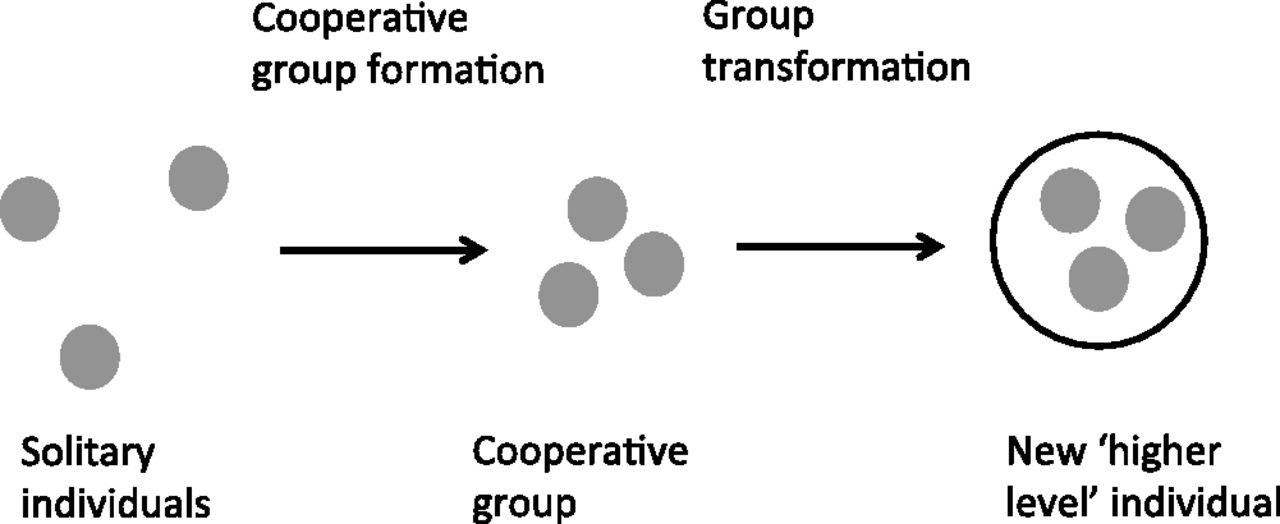
\includegraphics[width=\linewidth]{static/transition-west2015.jpg}
%     \end{subfigure}
    \tikz{            
    \node[accion] (i1) {} ;
    \node[accion, yshift=0.6cm, xshift=0.4cm] (i2) {} ;
    \node[accion, yshift=0.6cm, xshift=-0.4cm] (i3) {} ;
    \node[const, yshift=0.3cm, xshift=0.4cm] (i) {};
    
    \node[const, yshift=-0.8cm] (ni) {$\hfrac{\text{Individuos}}{\text{solitarios}}$};
    
    \node[const, yshift=1.2cm, xshift=1.5cm] (m1) {$\hfrac{\text{Formaci\'on}}{\text{de grupos}}$};
    
    \node[const, right=of i, xshift=2cm] (c) {};
    \node[accion, below=of c, yshift=0.35cm, xshift=0.4cm] (c1) {} ;
    \node[accion, above=of c, yshift=-0.35cm, xshift=0.6cm] (c2) {} ;
    \node[accion, above=of c, yshift=-0.35cm, xshift=0.2cm] (c3) {} ;
    \node[const, right=of c, xshift=0.6cm] (cc) {};
    
    \node[const, right=of ni, xshift=1.3cm] (nc) {$\hfrac{\text{Grupos}}{\text{cooperativos}}$};

    \node[const, right=of m1, xshift=1.2cm] (m2) {$\hfrac{\text{Transici\'on}}{\text{mayor}}$};
    
    \node[const, right=of cc, xshift=2cm] (t) {};
    \node[accion, below=of t, yshift=0.35cm, xshift=0.4cm] (t1) {} ;
    \node[accion, above=of t, yshift=-0.35cm, xshift=0.6cm] (t2) {} ;
    \node[accion, above=of t, yshift=-0.35cm, xshift=0.2cm] (t3) {} ;
    
    \node[const, right=of nc, xshift=1.1cm] (nt) {$\hfrac{\text{Unidad de}}{\text{nivel superior}}$};

    \edge {i} {c};
    \edge {cc} {t};
    
    \plate {transition} {(t1)(t2)(t3)} {}; %
    }
    \caption{Transiciones evolutivas mayores}
    \label{fig:transitions}
\end{figure}

\en{Some of the paradigmatic transitions are: from prokaryotic to eukaryotic cells; from protozoa to animals, plants and fungi (cell differentiation and emergence of multicellular organisms); and from solitary individuals to societies. }%
\es{Algunas de las transiciones paradigm\'aticas son: de las c\'elulas procariotas a las eucariotas; de los protozoa a los animales, plantas y hongos (diferenciaci\'on celular y emergencia de organismos multicelulares); y la formaci\'on de comunidades. }%
%
\en{From that moment until now, life has acquired an extraordinary complexity, both in terms of cooperation and specialization. }%
\es{Desde su origen hasta ahora, la vida adquiri\'o una extraordinaria complejidad, tanto a nivel de cooperaci\'on como de especializaci\'on. }%
%
\begin{figure}[ht!]
    \centering
    \begin{subfigure}[b]{0.5\textwidth}
    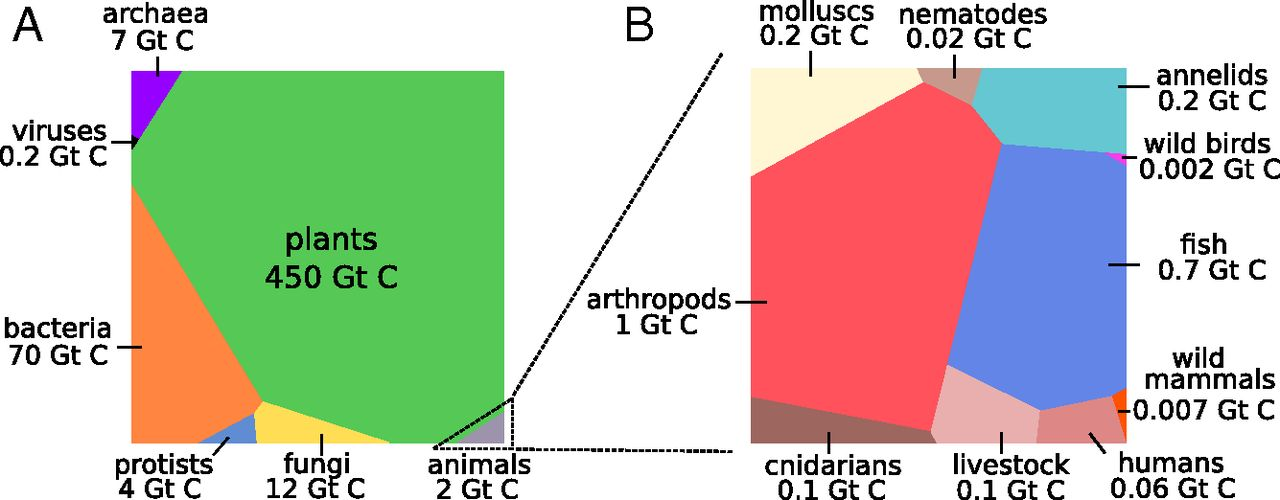
\includegraphics[width=\linewidth]{static/biomass.jpg}
    \end{subfigure}
    \caption{
    \en{Distribution of biomass on Earth estimated by Bar-On et al.~\cite{barOn2018-biomass}. }
	\es{Distribuci\'on de la biomasa en la Tierra estimada por Bar-On et al.~\cite{barOn2018-biomass}. }%
    }
    \label{fig:biomass}
\end{figure}
%
En la actualidad, el 82\% de la biomasa corresponde al reino de las plantas, el 13\% a las bacterias, el 2.2\% a los hongos, y 0.36\% a los animales, dentro de los cuales los humanos representamos el 3\%.
%
No es sorprendente que la plantas ocupen la mayor proporci\'on de la biomasa, pues ellas son las principales productoras primarias, capaces de generar materia org\'anica a partir de la luz solar, el agua y los gases de la atm\'osfera.
Las plantas realizan este complejo proceso de forma sumamente eficiente.
Este conocimiento est\'a almacenedado en su material gen\'etico, y no existe conocimiento cient\'ifico-t\'ecnico que sea capaz de imitar este proceso.
Los animales, hongos y el resto de heter\'otrofos, est\'an obligados a adquirir el material org\'anico de otros seres vivos, lo que los obliga a coexistir con sus presas, creando una compleja red de dependecias mutuas que constituyen la unidad de nivel superior mayor, los sistemas ecol\'ogicos.


\subsection{La función de costo evolutiva: los procesos multiplicativos}

\en{In evolution it is said that the growth of a lineage over time, $\omega(t)$, is governed by a stochastic sequence of survival and reproduction rates $f(\cdot)$ dependent on a random environment $\Aa$, }
\es{En evoluci\'on se dice que el crecimiento de un linaje en el tiempo, $\omega(t)$, esta gobernado por una secuencias de tasas de supervivencia y reproducci\'on $f(\cdot)$ dependientes de un ambiente aleatorio $\Aa$, }%
%
\begin{equation} \label{eq:modelo_exponencial}
\omega(T) = \prod_t^T f(\Aa(t)) \approx g^T
\end{equation}
%
\en{where $\Aa(t)$ represents the state of the environment at time $t$ and $g$ represents the characteristic growth rate when $T$ is sufficiently large. }%
\es{donde $\Aa(t)$ representa el estado del ambiente en el tiempo $t$ y $g$ representa la tasa de crecimiento caracter\'istica cuando $T$ es suficientemente grande. }%
%
Podemos interpretar $\omega(T)$ como el tama\~no de una poblaci\'on en el tiempo, pero tambi\'en esa poblaci\'on puede ser un recurso para otro linaje.
%
Por eso, de aqu\'i en adelante hablaremos de recursos, pero hay que mantener la idea de que este es un proceso al que est\'an sujeto el crecimiento de los linajes en general.
%
\en{For example, suppose nature flips a coin, if it comes up heads the population reproduces 50\% and if it comes up tails it survives 60\%. }%
\es{Por ejemplo, supongamos que la naturaleza lanza una moneda, si sale cara los recursos crecen \SI{50}{\percent} y si sale seca perdemos 40\%. }%
\begin{equation} \label{eq:estrategia_base}
f(\Aa) =
\begin{cases}
 1.5 & \Aa = \text{ \en{Head}\es{Cara} } \\
 0.6 & \Aa = \text{ \en{Tail}\es{Seca} }
\end{cases}
\end{equation}
%
\en{A similar example was proposed by Lewontin and Cohen (1969)~\cite{lewontin1969-randomlyVaryingEnvironment}. }%
\es{Un ejemplo similar fue analizado por Lewontin y Cohen (1969)~\cite{lewontin1969-randomlyVaryingEnvironment}. }%
%
% \en{Different strategies $\Ee$ can be described with different functions $f_\Ee(\Aa)$. }%
% \es{Diferentes estrategias $\Ee$ las podemos describr con diferentes funciones $f_\Ee(\Aa)$. }%
% %
% \en{According to the standard model of evolution, known as \emph{replicator dynamic} \cite{taylor1978-replicatorDynamic}, the change in the proportion of a strategy in the population, $x_\Ee$, is determined by its characteristic growth rate $g_\Ee$, }%
% \es{Seg\'un el modelo est\'andar de evoluci\'on, conocido como \emph{replicator dynamic} \cite{taylor1978-replicatorDynamic}, el cambio de la proporci\'on de una estrategia en la poblaci\'on, $x_\Ee$, est\'a determinado por su tasa de crecimiento caracter\'isitica $g_\Ee$, }%
% % schuster1983-replicatorDynamics, hofbauer2003-evolutionaryGameDynamics
% %
% \begin{equation} \label{eq:replicator_dynamic}  \tag{Replicator dynamic}
% \hspace{3cm} x_\Ee^\prime = \frac{x_\Ee g_\Ee}{\sum_i x_i g_i}
% \end{equation}
% %
% \en{where the denominator acts as a normalization constant. }%
% \es{donde el denominador act\'ua como constante de normalizaci\'on. }%
% %
\en{But, what is the characteristic growth rate $g$? }%
\es{¿Cu\'al es la tasa de crecimiento caracter\'istica $g$ en este caso? }%
%
\en{Much of the evolutionary literature considers that the correct estimate is obtained by the expected value, $g^t = \langle \omega \rangle_t$. }%
\es{Buena parte de la literatura en evoluci\'on considera que la estimaci\'on correcta se obtiene mediante el valor esperado, $g^t = \langle \omega \rangle_t$. }%
%
\begin{equation}
\langle \omega \rangle_t = \sum_{\omega \in \Omega_t} \omega \cdot  P(\omega)
\end{equation}
%
\es{Donde $\Omega_t$ es el conjunto de todas las posibles estados de $\omega$ en el tiempo $t$, y $P(\omega)$ es la la probabilidad de que el estado $\omega$ ocurra. }%
% 
\en{In the coin example, the expected value in the first two time steps is, }%
\es{En el ejemplo de la moneda, el valor esperado en los dos primeros pasos temporales es, }%
%
\begin{equation}
\begin{split}
\langle \omega \rangle_1 & = 1.5 \cdot \frac{1}{2} + 0.6 \cdot  \frac{1}{2} = 1.05 \\ 
\langle \omega \rangle_2 &=  1.5^2 \cdot \frac{1}{4} + 2 (0.6 \cdot 1.5 \cdot \frac{1}{4} ) + 0.6^2 \cdot \frac{1}{4}= 1.05^2
\end{split}
\end{equation}
%
\en{That is, the estimated growth rate according to the expected value is $5\%$ for each time step, $\langle \omega \rangle_t = 1.05^t$. }%
\es{Es decir, la tasa de crecimiento estimada seg\'un el valor esperado es de $5\%$ por cada paso temporal, $\langle \omega \rangle_t = 1.05^t$. }%
%
\en{And indeed that is what happens with the average of several individual trajectories, $\omega(t)$. }%
\es{Y efectivamente eso es lo que ocurre con el promedio de varias trayectoria individuales, $\omega(t)$. }%
%
\begin{figure}[ht!]
    \centering
    \begin{subfigure}[b]{0.45\textwidth}
    \includegraphics[width=\linewidth]{figures/pdf/ergodicity_expectedValue.pdf}
    \end{subfigure}
    \caption{
    \es{Promedio de los recursos (en escala logar\'itimica) a medida que aumentamos la cantidad de trayectorias individuales incluidas en el promedio (de $10^0$ a $10^4$). }%
    %
    \es{Cuando la cantidad de trayectorias individuales incluidas en el promedio es suficientemente grande, el promedio es igual al valor esperado $\langle \omega \rangle_t = 1.05^t$. }%
    }
    \label{fig:ergodicity_expectedValue}
\end{figure}
%
\en{When the individual trajectories can be described by the expected value of the system states, then the process is said to be ergodic~\cite{peters2019-ergodicityEconomics}. }%
\es{Cuando lo que le ocurre a los agentes individuales en el tiempo puede describirse mediante el valor esperado de los estados del sistema, luego se dice que el proceso es erg\'odico~\cite{peters2019-ergodicityEconomics}. }%
%
\en{However, the conditions are very restrictive, and are not fulfilled in the case of multiplicative processes. }%
\es{Sin embargo, las condiciones para que esto se cumpla son muy restrictivas y no se satisfacen en el caso de los procesos multiplicativos. }%
%
\es{Es decir, en nuestro ejemplo el valor esperado no representa lo que le ocurre en el tiempo a cada una de las trayectorias individuales por separado. }%
%
\es{Si bien las trayectorias individuales son variables (figura \ref{fig:ergodicity_individual_trayectories}), a largo plazo todas pierden a una tasa cercana al 5\% (figura \ref{fig:ergodicity_individual_trayectories_longrun}). }%
%
\begin{figure}[ht!]
    \centering
    \begin{subfigure}[b]{0.45\textwidth}
    \includegraphics[width=\linewidth]{figures/pdf/ergodicity_individual_trayectories.pdf}
    \caption{}
    \label{fig:ergodicity_individual_trayectories}
    \end{subfigure}
    \begin{subfigure}[b]{0.45\textwidth}
    \includegraphics[width=\linewidth]{figures/pdf/ergodicity_individual_trayectories_longrun.pdf}
    \caption{}
    \label{fig:ergodicity_individual_trayectories_longrun}
    \end{subfigure}
    \caption{
    \en{The black line represents the expected value. }%
    \es{La recta negra representan el valor esperado. }%
    %
    \en{Figure \ref{fig:ergodicity_individual_trayectories}: size of individual resources over time, $ \log(\omega(t))$. }%
    \es{Figura \ref{fig:ergodicity_individual_trayectories}: tama\~no de los recursos individuales en el tiempo, $ \log(\omega(t))$. }%
    %
    \en{Figure \ref{fig:ergodicity_individual_trayectories_longrun}: given enough time, all individual trajectories stick to the blue line. }% 
    \es{Figura \ref{fig:ergodicity_individual_trayectories_longrun}: con suficiente tiempo todas las trayectorias individuales se pegan a la recta azul. }% 
    }
    \label{fig:cpr_individual}
\end{figure}
%La relaci\'on entre el valor esperado y lo que le ocurre a los agentes individuales en el tiempo es un problema bien conocido en mec\'anica estad\'istica.
%
\en{To compute the growth rate $g$, we first express the product as follows, }%
\es{Para calcular la tasa de crecimiento $g$, primero expresaramos la productoria de la siguiente manera, }%
%
\begin{equation}
\omega(T) = \prod^T_{t=1} f(\Aa(t)) = f(\text{\en{head}\es{cara}})^{n_1} f(\text{\en{tail}\es{sello}})^{n_2}
\end{equation}
%
\en{where $n_1$ and $n_2$ represents the number of occurrences of $f(\text{\en{head}\es{cara}})$ and $f(\text{\en{tail}\es{sello}})$, with $n_1 + n_2 = T$. }%
\es{donde $n_1$ y $n_2$ representa la cantidad de ocurrencias de $f(\text{cara})$ y $f(\text{seca})$, con $n_1 + n_2 = T$. }%
%
\en{In the limit, $T \rightarrow \infty$ all individual trajectories will be determined by the same growth rate $g$. }%
\es{En el l\'imite, $T \rightarrow \infty$ todas las trayectorias individuales estar\'an determinadas por la misma tasa de crecimiento $g$. }%
%
\begin{equation} \label{eq:geometric_mean}
\begin{split}
\lim_{T \rightarrow \infty} \omega_e(T) & = {g}^T \\
\left( \lim_{T \rightarrow \infty} \omega_e(T) \right)^{1/T} & =  {g} \\
\lim_{T \rightarrow \infty} f(\text{cara})^{n_1/T} f(\text{seca})^{n_2/T} & 
 \end{split}
\end{equation}
%
\en{Where the frequencies $\frac{n_1}{T}$ and $\frac{n_2}{T}$ in the limit $T \rightarrow \infty$ are equal to the probabilities of the environmental states $p$. }%
\es{Donde las frecuencias $\frac{n_1}{T}$ y $\frac{n_2}{T}$ en el l\'imite $T \rightarrow \infty$ son iguales a las probabilidades de los estados ambientales $p$. }%
%
\en{Therefore, the growth rate is, }%
\es{Por lo tanto, la tasa de crecimiento es, }%
%
\begin{equation}
g = (1.5 \cdot 0.6)^{1/2} \approx 0.95
\end{equation}
%
\en{This formula, which allows computing the long-term growth rate of individual trajectories, has previously been used in the evolution literature under the name \emph{geometric mean}~\cite{dempster1955-geometricMean}. }%
\es{Esta f\'ormula, que permite computar la tasa de crecimiento a largo plazo de las trayectorias individuales, ha sido usada previamente en la literatura de evoluci\'on bajo el nombre de \emph{media geom\'etrica}~\cite{dempster1955-geometricMean}. }%
%
\en{The geometric mean is always less than the arithmetic mean (or expected value). }%
\es{La media geom\'etrica siempre es menor a la media aritm\'etica (o valor esperado). }%
%
\en{This is because in multiplicative processes the physical impacts of losses are usually stronger than those of gains. }%
\es{Esto se debe a que en los procesos multiplicativos los impactos f\'isicos de las p\'erdidas suelen ser m\'as fuertes que los de las ganancias. }%
%
\en{In an extreme case, a single zero in the product is enough to generate an extinction. }%
\es{En un caso extremo, un \'unico cero en la productoria alcanza para generar su extinci\'on. }%

% Decimos que un proceso es erg\'odico si se cumple que,
% \begin{equation}
%  \underbrace{\lim_{T \mapsto \infty} \frac{1}{T} \sum_{t=1}^T \omega(t)}_{\text{Media temporal}}  = \underbrace{\sum_{\omega} \omega \cdot p(\omega)}_{\text{Media de estados}}
% \end{equation}
% 

\subsection{Transiciones evolutivas mayores}

\es{Debido a que las fluctuaciones tienen un efecto negativo en las tasas de crecimiento individuales Yaari-Solomon~\cite{yaari2010-cooperationEvolution} y Peters-Adamou~\cite{peters-cooperation2019.03.04} estudian las consecuencias que el siguiente protocolo cooperativo tiene sobre la tasa de crecimiento de los agentes. }%
%
\begin{figure}[ht!]
\centering
\scalebox{0.75}{
\tikz{

    \node[latent, minimum size=2cm ] (x1_0) {$\omega(t)$} ;
    \node[latent, below=of x1_0, minimum size=2cm ] (x2_0) {$\omega(t)$} ;

    \node[latent, right=of x1_0, minimum size=3cm ] (x1_0g) {$ \omega(t)\cdot f(\Aa_1(t))$} ;
    \node[latent, right=of x2_0, minimum size=1.8cm, xshift=0.6cm , align=left] (x2_0g) {$\omega(t)\cdot$\\$f(\Aa_2(t))$} ;
    
    \node[latent, right=of x1_0g, minimum size=3.8cm, yshift=-1.33cm, align=right] (x_0) {$\omega(t)\cdot f(\Aa_1(t))$\\$+\omega(t)\cdot f(\Aa_2(t))$ } ;
    
    \node[const, above=of x_0] (nx_0) {$\overbrace{\text{Pool}\hspace{2.5cm}\text{Share}}^{\text{\normalsize Coopera\en{tion}\es{ci\'on}}}$} ;
    
    \node[latent, right=of x1_0g, minimum size=2.5cm,  xshift=4.5cm] (x1_1) {$\omega(t+1)$ } ;
    \node[latent, below=of x1_1, minimum size=2.5cm, yshift=0.7cm] (x2_1) {$\omega(t+1)$ } ;
    
    \edge {x1_0} {x1_0g};
    \edge {x2_0} {x2_0g};
    \edge {x1_0g,x2_0g} {x_0};
    \edge {x_0} {x1_1,x2_1};
    
}
}
\caption{
\en{The agents start with the same initial resources, update them independently according to the equation \ref{eq:estrategia_base}, and finally redistribute it in equal parts. }%
\es{Los agentes comienzan con los mismos recursos iniciales, los actualizan independientemente de acuerdo con la ecuaci\'on \ref{eq:estrategia_base}, y finalmente lo redistribuyen en partes iguales. }%
}
\label{fig:protocolo}
\end{figure}
%
Despu\'es de que cada agente actualiza sus recursos individuales, se ponen todos los recursos en un fondo com\'un que se divide en partes iguales.
%
Y se repite el proceso: se actualizan los recursos individualmente y se dividen en partes iguales.
%
La cooperaci\'on cambia la variable aleatoria de la que dependen las trayectorias individuales, de la moneda jugando individualmente, a la cuota que reciben del fondo com\'un jugando cooperativamente.
%
\begin{equation}
\omega(t+1) = \frac{1}{N}\left(n_c \, \omega(t) \, 1.5 + n_s \, \omega(t) \, 0.6\right)
\end{equation}
%
Donde $N$ es el tama\~no del grupo cooperativo, $n_c$ y $n_s$ la cantidad de caras y secas obtenidas en el grupo.
%
En el caso extremo en el que el $N=1$, la cuota del fondo com\'un es equivalente a los pagos generaos por la moneda.
%
Pero una caracter\'isitica del fondo com\'un es que tiene menos fluctuaciones que la moneda para todo $N>1$.
%
En el caso extremo, un grupo cooperativo de tama\~no infinito, la cuota es siempre equivalente a la media artim\'etica.
%
\begin{equation}
\omega(t+1) = \lim_{N\rightarrow \infty} \omega(t) \left(\frac{n_c}{N} 1.5 + \frac{n_s}{N} 0.6\right) = \omega(t)\,\underbrace{(p\,1.5 + (1-p)\,0.6)}_{\text{media aritm\'etica}}
\end{equation}


Las consecuencias de este protocolo sobre la tasa de crecimiento de los recursos son extraordinarias.
%
\es{La reducci\'on de las fluctuaciones producto de la mutua cooperaci\'on  en grupos de tama\~no finito genera un aumento en la tasa de crecimiento de todos sus miembros. }%
%
\en{In Figure \ref{fig:ergodicity_cooperation} we show the trajectory of an agent in a cooperating group of size 33. }%
\es{En la figura \ref{fig:ergodicity_cooperation} mostramos la trayectoria de un agente en un grupo cooperador de tama\~no 33. }%
%
\begin{figure}[ht!]
    \centering
    \begin{subfigure}[b]{0.45\textwidth}
    \includegraphics[width=\linewidth]{figures/pdf/ergodicity_cooperation.pdf}
    \end{subfigure}
    \caption{
    \en{The resources of an individual in a cooperative group of size 33 (green line) approaches the arithmetic mean (the black line below the green line).
    As a visual reference we show the geometric mean that drives the growth rate of individuals (blue line). }%
    \es{Los recursos de un individuo en un grupo cooperativo de tama\~no 33 (recta verde) se aproxima a la media aritm\'etica (la recta negra debajo de la recta verde).
    Como referencia visual mostramos la media geom\'etrica que gobierna la tasa de crecimiento de los individuos (recta azul). }%
    }
    \label{fig:ergodicity_cooperation}
\end{figure}
% 
\en{Individuals in fully cooperative groups achieve growth rates equivalent to the average of system states, which in non-ergodic systems is always higher than individual growth rates. }%
\es{Los individuos de los grupos enteramente cooperadores logran acceder a tasas de crecimiento cercanas al promedio de estados del sistema (media aritm\'etica), que en los sistemas multiplicativos siempre superior que la tasas de crecimiento individual (media geom\'etrica). }%
%
Para ganar intuición acerca de por qué la cooperación produce un aumento en la tasa de crecimiento puede ser \'util revisar lo que ocurre en un ejemplo básico.
%
En la siguiente comparamos lo que ocurre con los recursos de dos agentes no-cooperadores y dos agentes cooperadores.
%
\begin{table}[ht!]
\centering
 \begin{tabular}{|l|c|c|cc|c|cc|}
     \hline
         & {\small \, $\omega(0)$ } & {\small \  $f(\cdot) \ $}  & \multicolumn{2}{c|}{\small \, $\omega(1)$ } & {\small \  $f(\cdot) \ $} &  \multicolumn{2}{c|}{\small \,  $\omega(2)$ }  \\ \hline \hline
        A no-coop & $1$ & $1.5$ &  \multicolumn{2}{c|}{$1.5$} & $0.6$ & \multicolumn{2}{c|}{$\bm{0.9}$} \\ \hline
        B no-coop & $1$ & $0.6$ & \multicolumn{2}{c|}{$0.6$} & $1.5$ & \multicolumn{2}{c|}{$\bm{0.9}$}  \\ \hline\hline
         A coop & $1$ & $1.5$ & $1.5$ & $1.05$  & $0.6$ & $0.63$ & $\bm{1.1}$  \\ \hline
        B coop & $1$ & $0.6$ & $0.6$ & $1.05$ & $1.5$ & $1.57$ & $\bm{1.1}$ \\ \hline
\end{tabular}
\caption{Ilustración la actualización de los recursos en grupos no-cooperativos y cooperativos. La reducción de fluctuaciones en grupos cooperativos produce un aumento en la tasa de crecimiento de todos sus miembros. }
\end{table}
%
Los individuos comienzan con una unidad de recursos.
%
A obtiene Cara y Seca, y B obtiene Seca y Cara.
%
Cuando juegan no cooperativamente, ambos terminan con una riqueza menor a la que empezaron, pues en los procesos multiplicativos los impactos de la pérdidas son más importantes que los de las ganancias.
%
Cuando juegan cooperativamente, ambos terminan con una riqueza mayor a la que empezaron debido a la reducción de fluctuaciones individuales en cada paso.
%
\es{Este aumento puede parecer suficiente para creer que existe una ventaja a favor de la cooperaci\'on. }%
% %
% \en{However, they do not consider the problem of defection, who say ``our cooperators are unable to break the cooperative pact''. }%
% \es{Sin embargo ellos no consideran el problema de la deserci\'on, quienes dicen ``our cooperators are unable to break the cooperative pact''. }%
¿Qu\'e pasa si uno de los miembros decide dejar de aportar al fondo com\'un, pero sigue recibiendo su cuota del fondo com\'un?

% Parrafo

\en{In the last few decades evolutionary biology has begun to adopt the analogy of the ``tragedy of the commons''~\cite{rankin2007-tragedyCommonsBiology}. }%
\es{En las \'ultimas d\'ecadas la biolog\'ia evolutiva ha comenzado a adoptar la analog\'ia de la ``tragedia de los comunes''~\cite{rankin2007-tragedyCommonsBiology}. }%
%
\en{This concept contains the idea that the commons has a payoff structure isomorphic to the N-player prisoner's dilemma~\cite{hardin1971-collectiveAsPrisionerDilema}. }%
\es{Este concepto contiene la idea de que los bienes comunes tienen una estructura de pagos isomorfa al dilema del prisionero de N jugadores~\cite{hardin1971-collectiveAsPrisionerDilema}, donde desertar siempre es mejor que cooperar. }%
%
\en{\T }%
\es{Una matriz de pagos dilema del prisionero de dos jugadores t\'ipica tiene la siguiente estructura, }% 
%
\begin{equation}
  \bordermatrix{ & C & D \cr
      C & b-c & -c \cr
      D & b & 0 } 
\end{equation}
%
donde el beneficio es mayor al costo, $b > c$.
%
\en{Players gain more if they opt for mutual cooperation than for mutual defection, since $b - c > 0$. }%
\es{Los jugadores ganan m\'as si optan por la cooperaci\'on mutua que por la deserci\'on mutua, ya que $b - c > 0$. }%
%
\en{However, regardless of what the other player does, it is better not to cooperate: if my partner defects, it is better for me to defect than to cooperate, since $0 > -c$; if my partner cooperates, it is still better for me to defect than to cooperate, since $b > b - c$. }%
\es{Sin embargo, independientemente de lo que haga el otro jugador, es mejor no cooperar: si mi compa\~nero deserta, es mejor para m\'i desertar que cooperar, ya que $0 > -c$; si mi compa\~nero coopera, sigue siendo mejor para m\'i desertar que cooperar, ya que $b > b - c$. }%
%
\en{This creates a dilemma: although mutual cooperation is a preferable outcome, no individual has the incentive to cooperate. }%
\es{De ah\'i el dilema: aunque la cooperaci\'on mutua es un resultado preferible, ning\'un individuo tiene el incentivo de cooperar. }%

% Parrafo

\en{\T }%
\es{Si este fuera el caso, los desertores deber\'ian tener una tasa de crecimiento mayor a lo cooperadores. }%
%
\en{However, the first defector from an entirely cooperative group obtains a lower growth rate than before defecting. }%
\es{Sin embargo, en la figura~\ref{fig:ergodicity_desertion} podemos observar que el primer desertor de un grupo enteramente cooperador obtiene una tasa de crecimiento menor a la que ten\'ia antes de desertar. }% 
%
\begin{figure}[ht!]
    \centering
    \begin{subfigure}[b]{0.45\textwidth}
    \includegraphics[width=\linewidth]{figures/pdf/ergodicity_desertion.pdf}
    \end{subfigure}
    \caption{
    \en{The colors represent groups of size 100 with 0, 1 and 2 defectors. }%
    \es{Los colores representan los grupos de tama\~no 100 con 0, 1 y 2 desertores. }%
    %
    \en{The curves of the individual defectors are those at the top of each of the groups. }%
    \es{Las curvas de los individuos desertores son las que est\'an arriba en cada uno de los grupos. }%
    }
    \label{fig:ergodicity_desertion}
\end{figure}
%
\en{The resources of the first individual defector (blue group with 1 defector), is below the resources of the individuals in the fully cooperative group (green group with 0 defectors). }%
\es{Los recursos del primer individuo desertor (la curva variable del grupo azul), est\'a por debajo de los recursos de los individuos del grupo enteramente cooperador (grupo verde con 0 desertores). }%
%
\en{Defecting, instead of increasing the growth rate of the defective individuals, reduces it. }%
\es{Desertar, en vez de aumentar la tasa de crecimiento de los individuos desertores, la reduce. }%
%
\en{\T }%
\es{Esto ocurre cada vez que una agente cambia de comportamiento de cooperador a desertor (ver grupo rojo con dos desertores). }%
%
\en{Without penalties, defector strategies negatively affect their own long-term growth rate because their own behavior increases the fluctuations of the random variable on which they depend. }%
\es{Sin necesidad de introducir castigos, las estrategias desertoras afectan negativamente su propia tasa de crecimiento a largo plazo debido a que su comportamiento aumenta las fluctuaciones de la variable del fondo com\'un del que dependen.}
%
\en{In other words, the commons does not have the structure of the prisoner's dilemma, as is usually claimed in the literature. }%
\es{Es decir, los bienes comunes no tiene la estructura del dilema del prisionero como habitualmente se afirma en la literatura. }%
% 
% \en{This means that the payoff matrix is not isomorphic to a prisoner's dilemma. }%
% \es{Esto significa que la matriz de pagos no son isomorfas al dilema del prisionero. }%

% Parrafo

En cualquier caso, los desertores siempre tienen una posici\'on relativa mejor que los cooperadores de su propio grupo.
%
Esto puede favorecer la selecci\'on de comportamientos desertores al interior de los grupos, por ejemplo por imitaci\'on, produciendo una cascada de deserciones que pongan fin a toda cooperaci\'on.
%
Pero al mismo tiempo, la tasa de crecimiento m\'as alta la obtienen los grupos enteramente cooperativos, lo que favorece la selecci\'on de grupos enteramenete cooperadores sobre el resto.
%
\es{Por este motivo, la selecci\'on multinivel favorece a los individuos cooperadores sobre los desertores. }

\subsection{Evolución cultural}

La especial integraci\'on de los procesos biol\'ogicos, cognitivos y sociales que permiten a los humanos desarrollar culturas complejas se debi\'o a una coevoluci\'on gen\'etico-cultural desencadenada por el desarrollo previo de la crianza cooperativa~\cite{hrdy2020-emotionallyModern}.
La forma en la que estos homininos organizaron la crianza produjo un ambiente que favoreci\'o la selecci\'on de j\'ovenes capaces de monitorear y comprender las intenciones de los dem\'as, y de trasmitir a sus cuidadadores sus propias necesidades.
%A diferencia de nuestros parientes m\'as cercanos (chimpanc\'es, bonobos, gorilas y orangutanes)
Antes del surgimiento de los humanos anat\'omicamente modernos (masa cerebral actual) y de los humanos conductualmente modernos (lenguaje), surgi\'o en África una linaje emocionalmente moderno con capacidades para el entendimiento mutuo~\cite{hrdy2020-emotionallyModern}.

La comprensi\'on mutua, la imitaci\'on y el lenguaje permitieron la  transmisi\'on de conocimientos basados en la experiencia de otros (\emph{aprendizaje social}), dando inicio a un proceso cooperativo inter-generacional que produjo el desarrollo de \emph{las culturas}, sistemas de informaci\'on independiente al gen\'etico que permiti\'o a las poblaciones humanas adaptarse r\'apidamente a los cambiantes contextos ambientales.
El surgimiento de este nuevo sistema de informaci\'on produjo cambios radicales para nuestra especie.
Antes de la transici\'on cultural, estuvimos en grave peligro de extinci\'on, lo que se evidencia en la baja diversidad del genoma humano.
Luego de la transici\'on cultural, organizados en sociedades cazadores-recolectores, nuestra especie fue capaz de ocupar en pocos a\~nos todos los nichos ecol\'ogicos de la tierra como ning\'un otro vertebrado terrestre lo hab\'ia logrado antes.
Saliendo de África ocupamos Asia, Ocean\'ia y las Am\'ericas (Figura~\ref{fig:agricultura}).
% La informaci\'on transgeneracional fue la que le permiti\'o a estas sociedades simples adaptarse r\'apidamente a los nuevos desaf\'ios ecol\'ogicos.

\begin{figure}[ht!]
    \centering
    \begin{subfigure}[b]{0.6\textwidth}
     \includegraphics[width=\textwidth]{figures/agricultura.pdf}
     \label{fig:agricultura}
    \end{subfigure}
%     \begin{subfigure}[b]{0.40\textwidth}
%     \includegraphics[width=\textwidth]{static/polynesia.png} 
%     \caption{Poblamiento del oc\'eano Pac\'ifico}
%     \label{fig:polynesia}
%     \end{subfigure}
    \caption{
    Poblamiento humano (flechas) y surgimientos independientes de la agricultura (puntos).
    Proyecci\'on pol\'iedrica que conserva los tama\~nos relativos de la tierra.
    %Las felchas indican el poblamiento, desde África a Asia, y de Asia hacia Ocean\'ia y Am\'erica.
    %Los puntos rojos indican surgimiento independiente de agricultura.
    %El mapa de la figura~\ref{fig:polynesia}, desarrollado por Thorsby~\cite{thorsby2016-polynesiaAmerica}, muestra el poblamiento de la Polynesia y los contactos con Ámerica evidenciados en el material gen\'eticos.
    }%
    \label{fig:poblamiento}
\end{figure}

El cambio cultural es un fen\'omeno poblacional que emerge como consecuencia del intercambio de informaci\'on entre individuos.
%
\en{Based on the principles of evolutionary theory (descent, mutation and selection), a theoretical framework of ``cultural evolution'' has been developed to explain how culture changes over time. }%
\es{Basada en los principios de la teor\'ia de la evoluci\'on (descendencia, modificaci\'on y selecci\'on), se ha desarrollado un marco te\'orico de \emph{evoluci\'on cultural} que intenta explicar c\'omo cambia la cultura en el tiempo. }%
%
\en{Descent, mutation and selection of cultural information occurs when an individual adopts the behavior of others, either because it is the behavior of the majority (frequency-based strategy) or because the other individual is particularly successful or prestigious (payoff-based strategy). }%
\es{La descendencia, mutaci\'on y selecci\'on de la informaci\'on cultural se produce cuando una persona adopta el comportamiento de otras, sea porque es el comportamiento de la mayor\'ia o sea porque es la otra persona es particularmente exitosas o prestigiosas. }%
%
\en{All social learning processes modify to some degree the cultural variant adopted. }%
\es{Todos los procesos de aprendizaje social modifican en alg\'un grado la variante cultural adoptada. }%
%
\en{And some of these cultural variants spread faster or are more stable than others, predominating over time. }%
\es{Y algunas de esas variantes culturales se propagan m\'as r\'apido o son m\'as estables que otras, predominando en el tiempo. }%

% Parrafo

La experiencia acumulada a trav\'es de las generaciones por las m\'as diversas comunidades del mundo condujo, de forma independiente, al desarrollo de tecnolog\'ias de reciprocidad sorprendentemente similares entre s\'i.
%
La antropolog\'ia ha reconocido la existencia de una obligaci\'on universal de dar y de recibir.
%
De esta forma, el acto de donar, dar un regalo o hacer un favor activa un ciclo de intercambios a trav\'es de la obligaci\'on rec\'iproca para devolver de alguna forma lo recibido.
%
Este tipo de intercambios es la primera forma econ\'omica y es un mecanismo de flujo de bienes y servicios fundamental incluso en las sociedades modernas, a trav\'es de las que se establecen relaciones de correspondencia, hospitalidad, protecci\'on y asistencia mutua~\cite{mauss, polanyi, salins}.

% Parrafo

Si bien los intercambios rec\'iprocos ocurren generalmente de forma rutinaria, en todas las sociedades se pueden reconocer dos mecanismos que cumplen la funci\'on de re-ciclar los v\'inculos interprersonales: los ritos festivos y los ritos coercitivos~\cite{segato2016-guerraContraLasMujeres}.
%
Los ritos coercitivos, no son otra cosa que ceremonias para la reactivaci\'on de flujos de intercambios rotos previamente por conflictos entre partes.
%
Est\'an orientados el restablecimiento de los v\'inculos mediante los mecanismos de ``reparaci\'on'', ``conciliaci\'on'' y ``ayuda'' \cite{zaffaroni2013-cuestionCriminal}, nombre relativamente arbitrarios para los tres tipos de intercambios posibles entre partes: dar ($\rightarrow$), intercambiar ($\leftrightarrow$) y recibir ($\leftarrow$).
%
La expulsi\'on del agresor de la comunidad s\'olo se prevee en casos extremadamente excepcionales, pues el primer derecho de sus miembros es formar parte de la comunidad \cite{segato2016-guerraContraLasMujeres}.

% Parrafo

Las tecnolog\'ias de reciprocidad social son fundamentales para la supervivencia de las comunidades en el tiempo, pues ellas reducen las fluctuaciones individuales que ponen en peligro su estabilidad.
%
La teor\'ia de la probabilidad nace en 1648 justamente como respuesta a la pregunta de cu\'al es el \emph{precio justo} en contextos de incertidumbre.
%
El problema analizaban Pascal y Fermat en sus cartas es equivalente al siguiente.
%
Tiramos dos veces la moneda.
%
Si sale seca $S$ en la primera y en la segunda, una persona (en rojo) le hace un favor a la otra.
%
En caso contrario, el favor se invierte.
%
¿Cu\'al es el valor justo de la reciprocidad en este contexto de incertidumbre?

\begin{figure}[ht!]
    \centering
    \tikz{
    \node[latent, draw=white, yshift=0.7cm, minimum size=0.1cm] (b0) {};
    \node[latent,below=of b0,yshift=0.7cm, xshift=-1cm] (r1) {$S$};
    \node[latent,below=of b0,yshift=0.7cm, xshift=1cm] (r2) {$C$};

    \node[latent, below=of r1, draw=white, yshift=0.8cm, minimum size=0.1cm] (bc11) {};
    \node[accion, below=of r2, draw=white, yshift=0cm, color=blue!70] (bc12) {};
    \node[latent,below=of bc11,yshift=0.8cm, xshift=-0.5cm] (r1d2) {$S$};
    \node[latent,below=of bc11,yshift=0.8cm, xshift=0.5cm] (r1d3) {$C$};

    \node[accion,below=of r1d2,yshift=0cm, color=red!70] (br1d2) {};
    \node[accion,below=of r1d3,yshift=0cm, color=blue!70] (br1d3) {};
    \edge[-] {b0} {r1,r2};
    \edge[-] {r1} {bc11};
    \edge[-] {r2} {bc12};
    \edge[-] {bc11} {r1d2,r1d3};
    \edge[-] {r1d2} {br1d2};
    \edge[-] {r1d3} {br1d3};
    }
    \caption{El problema del \emph{valor justo} que da inicio a la teor\'ia de la probabilidad}
    \label{fig:pascal-fermat}
\end{figure}

La respuesta a la que arribaron Pascal y Fermat es que el valor de los favores tiene que ser inversamente proporcional a la probabilidad de hacer el favor.
%
Si la moneda es no sesgada, hay 1/4 de probabilidad de que salgan dos secas (terminal roja), 1/4 de que salga seca en la primera y cara en la segunda (terminal azul) y 1/2 de que salga cara en la primera (terminal azul).
%
Luego, la probabilidad de que la persona azul haga un favor es 3/4.
%
Si la persona roja hace favores por un valor equivalente a 4, el azul tiene que devolver los favores con un valor de 4/3, una relaci\'on de 3 a 1.
%
Esta forma intuitiva de calcular la probabilidad de un conjunto de eventos mutuamente excluyentes, como suma de sus probabilidades elementales, constituye el axioma fundamental de Kolmogorov a partir del cual se puede montar toda la teor\'ia de la probabilidad.

% Parrafo

De forma similar a las tecnolog\'ias de reciprocidad social, las tecnolog\'ias de reciprocidad ecol\'ogica promueven la coexistencia con las especies de las cuales dependemos garantizando as\'i la supervivencia de la comunidad en el tiempo.
%
Los estudios comparados indican que las instituciones capaces de interactuar de forma estable con los sistemas ecol\'ogicos siempre son de tipo comunitario, basados en normas que condensan la acumulaci\'on conocimiento experto resultado de un largo proceso inter-generacional de evoluci\'on cultural local~\cite{ostrom1990}.
% 
El remplazo repentino de estos sistemas culturales locales por instituciones modernas externas, privadas o p\'ublicas, produce generalmente desequilibrios en los sistemas ecol\'ogicos por sobre explotaci\'on de los recursos, reduciendo el tama\~no m\'aximo de poblaci\'on que el ambiente puede soportar~\cite{ostrom2010}.

% Parrafo

Los pueblos bien adaptados para la coexistencia intercultural y ecol\'ogica practican cosmovisiones basadas en l\'ogicas paraconsistentes que les permite creer en A y no A al mismo tiempo.
Estas cosmovisiones, que obligan a no rechazar ninguna alternativa aunque se tenga preferencia por alguna, son la base de toda tecnolog\'ia de reciprocidad con la biocenosis en todo el mundo, como son los ritos \emph{Canang sari} practicados en Bali o como los ritos \emph{pacham\'amicos} practicados en Am\'erica del sur.
\begin{figure}[ht!]
    \centering
    \begin{subfigure}[b]{0.45\textwidth}
    \centering
    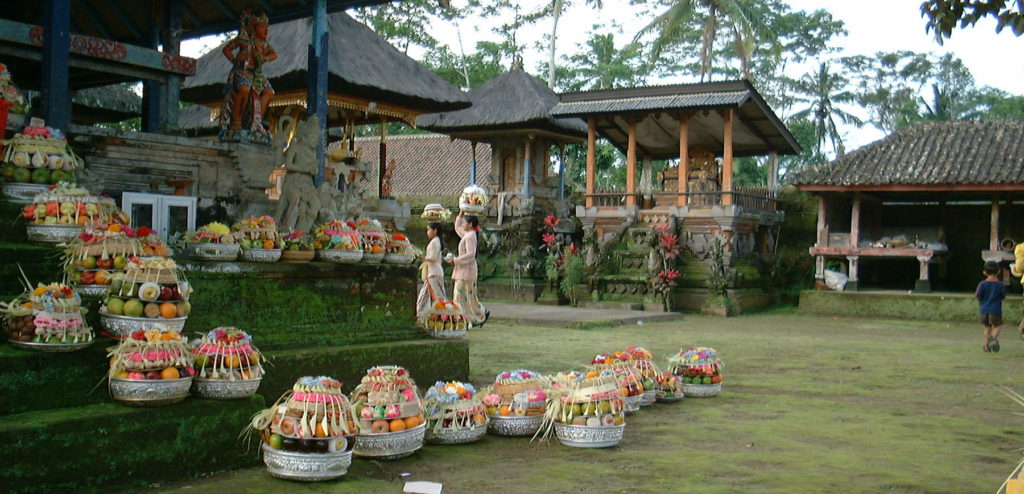
\includegraphics[width=\linewidth]{static/bali-offerings}
    \caption{Canang sari}
    \label{}
    \end{subfigure}
    \begin{subfigure}[b]{0.3\textwidth}
    \centering
    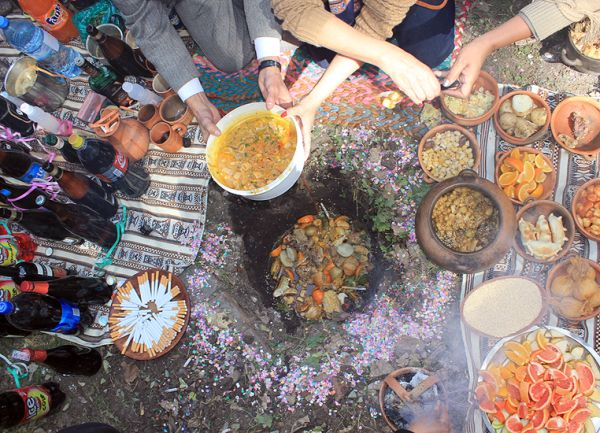
\includegraphics[width=\linewidth]{static/pachamama}
    \caption{Pachamama}
    \label{}
    \end{subfigure}
    \caption{Tecnolog\'ias de reciprocidad socio-ecol\'ogicas.}
    \label{fig:mito}
\end{figure}
Estas cosmovisiones basadas en l\'ogicas paraconsistentes obliga al ser humano a fomentar la coexistencia con otras formas de vida, como con otras culturas.

% Parrafo

Las tecnolog\'ias de reciprocidad ecol\'ogica produjeron la aparici\'on independiente de la domesticaci\'on de especies animales y vegetales, el desarrollo de caracteres gen\'eticos especiales que surgen como resultado de una interacci\'on prolongada entre las especies.
%
En particular, la reciprocidad con las especies fotosint\'eticas (\emph{agricultura}), \'unicas con la capacidad de producir materia org\'anica a partir del sol y la materia inorg\'anica, produjo nuevamente cambios radicales para nuestra especie.
%
La agricultura impuls\'o un marcado aumento poblacional.
%
Y el aumento de la poblaci\'on promovi\'o, a su vez, el desarrollo de nuevas innovaciones tecnol\'ogicas y cient\'ificas, como la escritura, la matem\'aticas, las ingenier\'ias, la astronom\'ia, las ciencias pol\'iticas, entre otras.

% Parrafo

La agricultura surgi\'o de manera de forma paralela en los seis grandes sistemas geogr\'aficos de la tierra: en la regi\'on central de África subsahariana, en Asia occidental, en Asia oriental, en Ocean\'ia norte, en Am\'erica del norte y en Am\'erica del sur (las puntos rojos de la figura~\ref{fig:agricultura}).
%
Alrededor de estos puntos se desarrollaron los principales centros poblacionales de la humanidad.
%
Durante el a\~no 1400 el mundo florec\'ia de sociedades "pr\'osperas"~\cite{dussel2004-sistemaMundo}: Aztecas en Ámerica del norte, Incas en Ámerica del sur, Tongas en el Pac\'ifico, Bant\'ues en África sub-sahariana, los Árabes e Indios en Asia occidental y Chinos en Asia oriental, por mencionar algunos.
%
El desarrollo tecnol\'ogico de todas estas sociedades fue extraordinario. 
%
% El imperio de Tonga ocupaba hace siglos todo el oc\'eano Pac\'ifico (figura~\ref{fig:polynesia}) con tecnolog\'ias de navegaci\'on que le hab\'ian permitido tener intercambios con Am\'erica de Sur~\cite{thorsby2016-polynesiaAmerica, ioannidis2020-polynesiaAmerica}.
% %
% En Am\'erica del Sur se hab\'ia desarrollado un sistema de intercambios basado en la reciprocidad de trabajo (minka, ayni y mita) que le permit\'ia a las comunidades administrar eficientemente el uso de los bienes comunes y al Estado desarrollar la infrastructura en el vasto territorio monta\~noso~\cite{murra1978-organizacion}.
% %
% En la regi\'on Azteca se hab\'ia desarrollado un extenso mercado regional con ciudades de hasta 300.000 habitantes, tres veces la ciudad de Venecia en esa misma \'epoca.%~\cite{www7.uc.cl}. %http://www7.uc.cl/sw_educ/historia/conquista/parte1/html/h54.html
% %
% El mundo \'Arabe comerciaba productos desde el Oc\'eano Pac\'ifico, en las Filipinas, hasta el Oc\'eano Atl\'antico, en Marruecos, conectando las innovaciones culturales de distintos hemisferios del planeta~\cite{dussel2004-sistemaMundo}.
% %
África siempre fue el continente m\'as diverso cultural y gen\'eticamente, pero quiz\'as el centro m\'as innovador en t\'erminos cient\'ificos y tecnolog\'ias haya sido la regi\'on de China~\cite{needham2004-generalConclusionsAndReflections}.

% Parrafo

\subsection{Ciencia colonial-moderna}

John Needham, el brit\'anico que dedic\'o su vida a recopilar la monumental historia cient\'ifica y t\'ecnica de China, reconoce que comenz\'o a estudiar el tema motivado por responder la pregunta de por qu\'e s\'olo Europa occidental hab\'ia logrado el avance cient\'ifico.
\begin{quotation}
When I first formed the idea, about 1938, (...) I regarded the essential problem as that of why modern science had not developed in Chinese civilisation (or Indian or Islamic) but only in that of Europe~\cite{needham2004-generalConclusionsAndReflections}.%
\end{quotation}
Luego de 60 a\~nos de investigaciones, Needham se ve obligado inviertir la pregunta.
\begin{quotation}
Why, between the -1th century and the 15th century, was Chinese civilisation much \emph{more} efficient than occidental in gaining natural knowledge and in applying it to practical human needs?~\cite{needham2004-generalConclusionsAndReflections}
\end{quotation}

% Parrafo

Desde Hegel hasta la fecha, las explicaciones euroc\'entricas intentan explicar la proposperidad actual de occidente a trav\'es de una causa interna: la ``\'etica protestante'' de Max Weber~\cite{weber1905-eticaProtestante}, la ``mentalidad burguesa'' de Jos\'e Luis Romero~\cite{romero1967-revolucionBurguesa}, o m\'as recientemente el ``sistema de parentezco'' de Joseph Henrich~\cite{henrich2020-weirdest}.
La paradoja que no puede responder la f\'abula euroc\'entrica es c\'omo una sociedad sumida en un proceso de involuci\'on cultural \'unico, como la sociedad feudal de la ``edad media'', pudo generar de repenten el extraordinario proceso de desarrollo cient\'ifico y t\'ecnico de la modernidad.

% Parrafo

As\'i como la integraci\'on favorece los proceso de innovaci\'on y acumulaci\'on cultural, el asilamiento induce p\'erdidas masivas de informaci\'on cultural.
%
Un ejemplo paradigm\'atico de aislamiento total ocurre con la separaci\'on de Tasmania del continente Australiano por la subida del nivel del mar ocurrida a comienzos del Holonceno.
%
La evidencia arqueol\'ogica y etnohist\'orica indica que desde el principio del Holoceno las sociedades de Tasmania perdieron gran parte de su cultura tecnol\'ogica.
La principal hip\'otesis sugiere que la reducci\'on del tama\~no efectivo de la poblaci\'on fue la causa de la p\'erdida cultural~\cite{Henrich2004}.
%
La capacidad de almacenamiento (e innovaci\'on) de tecnolog\'ias complejas, incluso aquellas desarrolladas por las sociedades cazadoras-recolectoras, requiere de un tama\~no m\'inimo de la poblaci\'on que s\'olo se puede alcanzar a trav\'es de la coexistencia entre distints pueblos con identidad propia.

% Parrafo

Un caso de asilamiento parcial ocurre en Europa occidental durante la Edad Media.
%
Antes de que tuviera lugar la Edad Media, el Imperio Romano produjo una p\'erdida masiva de diversidad cultural en su entorno, que tuvo consecuencias cr\'iticas para esta sociedad.
%
Arrinconada ya en el lejano occidente por el fr\'io polar y la falta de tecnolog\'ias de navegaci\'on del Atl\'antico, Europa occidental comienza en el siglo octavo a quedar paulatinamente aislada del ``sistema mundo'' por la expansi\'on Árabe al sur y por la serie cismas con el Imperio Romano de Oriente~\cite{Dussel}.
%
Aislada pacialmente del sistema mundo, esta sociedad entra en un proceso de involuci\'on cultural que condujo a un deterioro extremo de las condiciones de vida.

\begin{figure}[ht!]     
  \centering 
  \begin{subfigure}[c]{0.45\textwidth}
    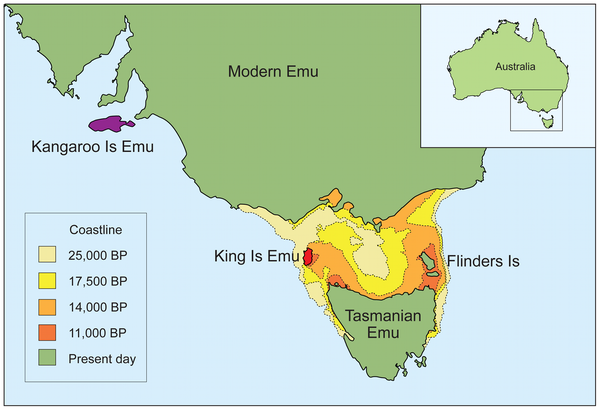
\includegraphics[width=\textwidth]{static/tasmania.png} 
    \caption{Tasmania}
    \label{fig:tasmania}
  \end{subfigure}
  \begin{subfigure}[c]{0.45\textwidth}
    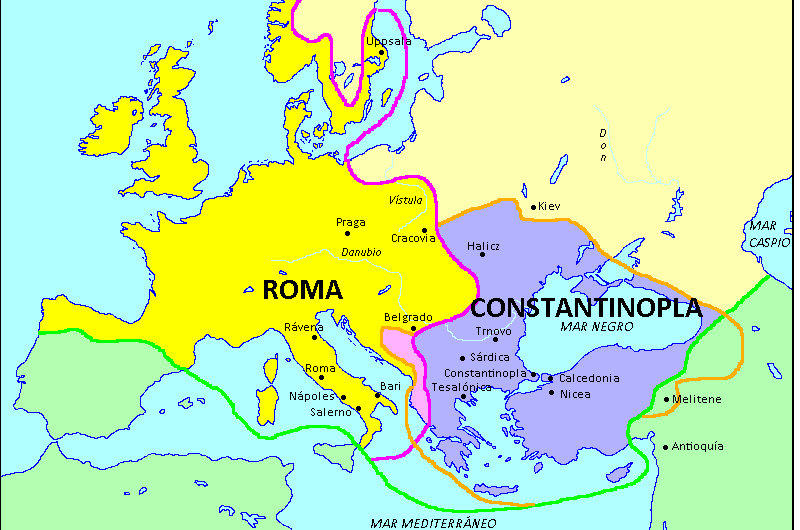
\includegraphics[width=\textwidth]{static/cisma.png} 
    \caption{Edad media}
    \label{fig:cisma}
  \end{subfigure}
  \caption{Aislamiento}
  \label{fig:aislamiento}
\end{figure}

En la etapa de aislamiento comenz\'o a ganar terreno al interior de la sociedad feudal el criterio de autoridad (religiosa, militar, acad\'emica, econ\'omica, sexual) como fundamento del ``saber aut\'entico''.
A pesar de la involuci\'on cultural generalizada, durante la Edad Media las instituciones heredadas del Imperio Romano de Occidente, en cabeza de la Iglesia Cat\'olica Romana, comenzaron a competir con las comunidades ind\'igenas locales y a producir una conjunto de novedosas tecnolog\'ias de colonizaci\'on~\cite{zaffaroni2013-cuestionCriminal}.
La primera y m\'as importante fue la regulaci\'on de las relaciones comunitaria de reproducci\'on (matrimonios) de forma m\'as detallada que la propiedad.
Se proscribe as\'i el rol pol\'itico que las mujeres desempe\~nan en el espacio dom\'estico comunitario, interviniendo en el funcionamiento de sus tecnolog\'ias de sociabilidad.

% Parrafo

%El avance colonial estuvo (y est\'a) motivado principalmente por una deficiencia social m\'as que por una puramente material.
La poblaci\'on desertora de las comunidades que pierden el arraigo comunitario pasan a sumarse como mano de obra para las actividades militares contra otros pueblos.
El mandato universal de exhibir p\'ublicamente alguna forma de poder para adquirir el estatus masculino hizo que los hombres derrotados se volvieran vulnerables al ejemplo de las masculinidades victoriosas.
Con el debilitamiento de los v\'inculos comunitarios, la cosmovisi\'on colonial e instrumental logra introducirse, cosificando todas las formas de vida.

% Parrafo

El poder punitivo se fue extendiendo y un nuevo sistema penal re-naci\'o de los llamados \emph{libris terribilis} del Digesto, antiguas leyes romanas recolectadas por encargo del emperador Justiniano de Constantinopla pero re-interpretadas en occidente de modo de liberar al poder punitivo de todo l\'imite.
En esta etapa, el sujeto masculino se torna modelo de lo humano y de todo cuanto sea dotado de politicidad, inter\'es general y valor universal, y el espacio de las mujeres se transforma en margen y resto de la pol\'itica.
La guerra contra las mujeres se formaliza definitivamente con la publicaci\'on del \emph{Malleus maleficarum} en 1484, que ser\'a el segundo best seller despu\'es de la Biblia durante los siguientes 200 a\~nos.

% Parrafo

% Producto de la p\'esima situaci\'on socio-econ\'omica, la sociedad fedual intenta varias veces, sin \'exito, recuperar la integraci\'on al sistema mundo por el oriente.
% Por lo tanto, la \'unica opci\'on que quedaba era explorar los mares del este.
% Hab\'ia mejores tecnolog\'ias de navegaci\'on en el mundo Árabe, en China y en el imperio de Tonga.
% Pero a diferencia de esos casos, apenas la sociedad fedual logra navegar el Atl\'antico, se desata un proceso migratorio t\'ipico de cualquier sociedad sumida en un proceso de grave violencia interna.
% El flujo migratorio europeo hacia am\'erica comienza a finales del siglo 15 y termina reci\'en a mediados del siglo 20.

Producto de la p\'esima situaci\'on socio-econ\'omica, apenas Europa occidental logra navegar el Atl\'antico, comienza un proceso migratorio t\'ipico de cualquier sociedad sumida en un proceso de grave violencia interna y degradaci\'on social, un flujo migratorio que comienza a finales del siglo 15 y termina reci\'en a mediados del siglo 20.
%Adem\'as de la buena predisposici\'on con la que los exploradores reportan haber sido recibidos por los habitantes Americanos, l
La llegada de masiva de emigrantes feudales produjo una serie de pandemias en Am\'erica que redujeron la poblaci\'on local en al menos un 66\% entre los a\~nos 1500 y el 1600~\cite{koch2019-europeanArrival}.
Un siglo antes, China hab\'ia incorporado la plata como monedad oficial, la que ya estaba siendo utilizada en todo el mundo Árabe~\cite{pomeranz2000-divergence, pomeranz2018-tradeCreated}.
El Estado Incaico, que estaba organizado en base a un sistema de intercamios reciproicitarios no monetarios, se encontraba era una regi\'on monta\~nosa rica en plata.
Cuando 1546 los exploradores descubren la monta\~na de plata de Potos\'i, en el centro del sistema estatal incaico, la Europa feudal queda inmediatamente en una posici\'on de privilegio en todo el mundo afro-euro-asi\'atico.

% Parrafo

El acceso a la plata americana produce un giro geopol\'itico.
La sociedad feudal rompe el cerco que la ten\'ia asilada del sistema mundo 25 a\~nos despu\'es de haber descubierto la monta\~na de plata de Potos\'i, y 80 a\~nos despu\'es de haber logrado navegar el Atl\'antico, en la batalla de Lepanto.
La plata, que ya era reconocida como moneda oficial en todo el mundo eruo-asi\'atico, coloc\'o de repente a esta sociedad marginal en una situaci\'on de integraci\'on privilegiada al sistema mundo.
La plata de Am\'erica fluye en todas las direcciones, principalmente en direcci\'on a China, y se inicia un proceso r\'apido de acumulaci\'on cultural basado en las tecnolog\'ias extranjeras.
%El proceso de involuci\'on cultural producto del asilamiento al sistema mundo durante la Edad Media, dio lugar a un proceso de r\'apidas innovaciones cient\'ificas y t\'ecnicas a partir de la integraci\'on privilegiada generada por el acceso a la plata, moneda de cambio en todo el continente afro-euro-asi\'atico.

% Parrafo

\begin{figure}[ht!]     
  \centering 
  \begin{subfigure}[b]{0.48\textwidth}
    
\includegraphics[width=\textwidth]{static/plata-potosi} 
    \caption{Plata}
    \label{fig:potosi}
  \end{subfigure}
   \ \ 
  \begin{subfigure}[b]{0.47\textwidth}
    \includegraphics[width=\textwidth]{figures/china.pdf} 
   \caption{Opio}
    \label{fig:china-pop}
  \end{subfigure}
  \caption{La plata y el opio como las llaves de la integraci\'on privilegiada de la Europa occidental en el sistema mundo.}
  \label{fig:integracion}
\end{figure}

% Parrafo

Durante 250 a\~nos la plata americana sirvi\'o para muchas cosas, pero principalmente para comprar productos chinos que impulsan la primera industrializaci\'on brit\'anica.
Europa consum\'ia productos asi\'aticos, pero exportaba muy poco a Asia.
El comercio internacional de opio comenz\'o a mediados del 1700 como respuesta a una crisis del comercio internacional europeo, especialmente brit\'anico.
El opio, un producto lujoso utilizado en China como medicina (raramente como estupefaciente), fue prohibida por los emperadores chinos en 1729, que por su abundancia hac\'ia crecer lentamente la cantidad de adictos.
Las consecuencias fueron m\'as graves cuando en 1818 se desarrolla una mezcla de opio m\'as barata y potente.

% Parrafo

Mediante el narcotr\'afico Europa occidental consigue por primera vez, reci\'en en el siglo 19, revertir el d\'eficit comercial que hist\'oricamente tuvo con China.
El n\'umero de adictos lleg\'o a ser lo suficientemente alarmante, y en 1839 China comete el error de declarar la guerra al narco-estado brit\'anico en su propio territorio.
Los resultados fueron terribles.
No s\'olo no pudieron impedir el ingreso de la droga.
Perdieron tambi\'en su autonom\'ia arancelaria, el derecho a someter a los residentes extranjeros a la ley China.
Expuesta a su debilidad militar, China sufri\'o un siglo calamitoso de agresiones extranjeras, desorden interno y guerra civil, que produjo una ca\'ida de 1/5 de su poblaci\'on (figura~\ref{fig:china-pop}).

% Parrafo

Luego de la derrota de China por parte del narco-estado brit\'anico, se establece por primera vez la hegemon\'ia de Europa occidental en el sistema mundo y comienza un proceso de colonizaci\'on en todo el mundo.
%, que hasta el momento estaba limitado a Am\'erica continental estaba limitada a puertos e islas.
En 1850 comienza la colonizaci\'on de África continental y de los extensos territorios americanos que todav\'ia segu\'ian a manos de comunidades locales.
Comienza la era de los genoentocidios.
\begin{figure}[ht!]
    \centering
    \begin{subfigure}[b]{0.48\textwidth}
    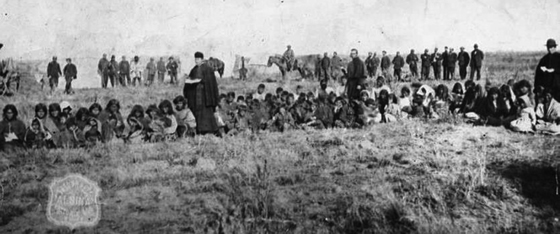
\includegraphics[width=\linewidth]{static/genocidio_patagonia}
    \caption{Genoetnocidios}
    \label{fig:genocidio_patagonia}
    \end{subfigure}
    \begin{subfigure}[b]{0.47\textwidth}
    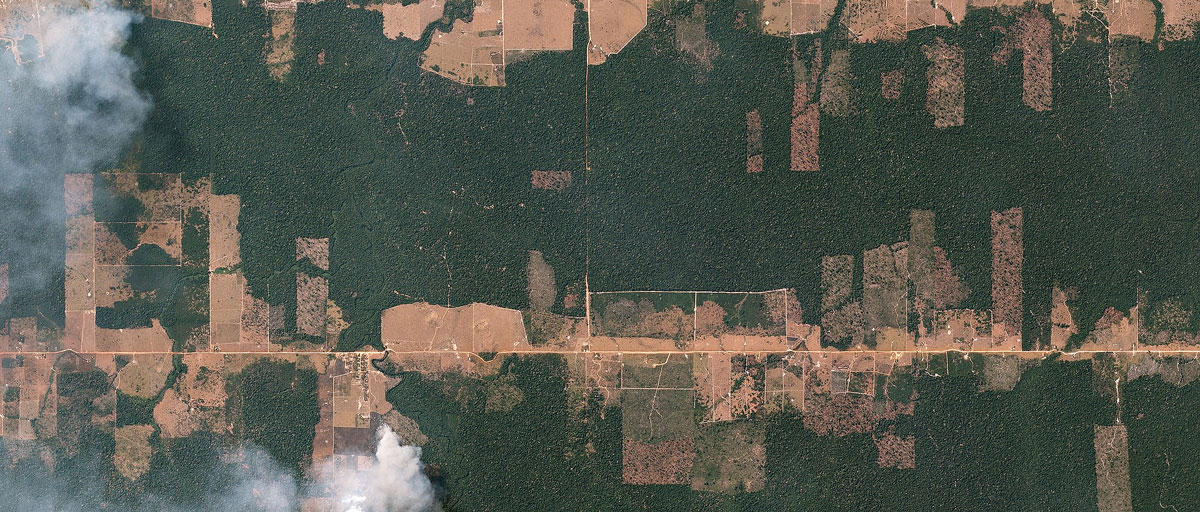
\includegraphics[width=\linewidth]{static/deforestation-brazil}
    \caption{Crisis ecol\'ogica}
    \label{fig:deforestation-brazil}
    \end{subfigure}
    \caption{
    La masiva p\'erdida de diversidad cultural trajo como consecuencia la masiva p\'erdida de biodiversidad actual, una crisis ecol\'ogica sin precedentes.
    }
    \label{fig:cultural-lose}
\end{figure}
En todas las partes del globo, los exploradores y etn\'ografos fueron documentando la perdida de cultural debida al avance del frente colonial-moderno, estatal o privado, sobre las autonom\'ias locales.
Es una nueva era de avances cient\'ificos y tecnol\'ogicos, pero por otro es la era de p\'erdida de diversidad cultural.
A pesar de todos los avances cient\'ificos, la ciencia metropolitana moderna no fue capaz de compensar la p\'erdida de los conocimientos milenarios acumulados por las comunidades aut\'onomas locales.
La masiva p\'erdida de diversidad cultural trajo como consecuencia la masiva p\'erdida de biodiversidad actual (figura~\ref{fig:deforestation-brazil}).
Quiz\'a la coexistencia sea la \'unica estrategia evolutivamente estable, y quienes la rompan sufran tarde o temprano las consecuencias.

% Parrafo

\section{Propiedades de los procesos multiplicativos}

Si los procesos multiplicativos gobiernan el desarrollo de los sistemas vivos, entonces las transformaciones evolutivas favorecerán aquellas estructuras y conductas que modifiquen las tasas de reproducción y supervivencia involucradas en el crecimiento a largo plazo de los linajes.
%
%Las formas mediantes las cuales los organismos vivos lo
Para estudiar algunas de las propiedades de los procesos multiplicativos analizaremos un juego de apuestas, en el que una casa de apuestas ofrece pagos $Q_c$ y $Q_s$ por Cara y Seca sobre una moneda con frecuencia $p$.
%
En este ejemplo tenemos un medio ambiente aleatorio (la moneda) y un intercambio entre al menos dos agentes: la casa de apuesta y quenes apuestan.

% Parrafo

Individualmente hay dos formas de apostar.
%
La primera es apostar a una \'unica de las dos opciones, por ejemplo a Caras.
%
En este escenario, la persona asigna un valor $ 1 \geq b_c = l > 0 $ a Caras y $b_s = 0$ a secas.
%
Supongamos que en la primera sale Cara y en la segunda Seca.
%
La riqueza en la primera es el ahorro $1-l$ m\'as el pago que obtiene por lo apostado en Cara $l \, Q_c$.
%
Y en la segunda vuelta, cuando sale Seca, la riqueza es solo el ahorro, lo no apostado a Cara $1-l$.
%
\begin{equation}
\omega_T = \underbrace{\overbrace{(\omega_0 \, (1-l) + \omega_0 \, l \, Q_c )}^{\omega_1} \, (1-l)}_{\omega_2} \,\dots
\end{equation}
%
Lo que podemos reescribir como,
%
\begin{equation}
\begin{split}
\omega_T &= \omega_0 \, ((1-l) + \, l \, Q_c ) \, (1-l) \, \dots \\
 &= \omega_0 \, ( (1-l) + \, l \, Q_c )^{n_c} \, (1-l)^{n_s} 
\end{split}
\end{equation}
%
donde $n_c + n_s = T$ son la cantidad de veces que sali\'o Cara y Seca en los $T$ pasos.
%
Es decir, la riqueza se actualiza siguiendo un proceso multiplicativo.

% Parrafo

La otra forma de apostar consiste en utilizar todos los recursos en cada vuelta, poniendo $b_c = b$ en Cara y el resto en Seca $b_s = (1-b)$.
%
En este caso la riqueza se actualiza como,
%
\begin{equation} \label{eq:kelly_paraconsistente}
\omega_T = \underbrace{\overbrace{(\omega_0 \, b \, Q_c)}^{\omega_1} \,  (1-b) \, Q_s}_{\omega_2} \dots = \omega_0 (b \, Q_c)^{n_c} ((1-b) \, Q_s )^{n_s}
\end{equation}
%
No s\'olo las dos formas de apostar actualizan los recursos a trav\'es de un proceso multiplicativo. 
%
No es dif\'icil demostrar que existe una equivalencia.
%
Por ello, de aqu\'i en adelante analizaremos \'unicamente esta \'ultima forma de apostar, la que utiliza todos los recursos en cada vuelta.

\subsection{La ventaja de la diversificación individual (propiedad epistémica)}

En general, la casa de apuestas puede ofrecer cualquier tipo de pago.
%
La tasa de crecimiento individal para cualquier pago no negativo, $Q_c > 0$ y $Q_s > 0$ es
%
\begin{equation}
\begin{split}
\lim_{T \rightarrow \infty } \omega_0 \, r^T &= \lim_{T \rightarrow \infty } \omega_0 (b \, Q_c)^{n_c} ((1-b) \, Q_s )^{n_s} \\
r &= \lim_{T \rightarrow \infty } (b \, Q_c)^{\frac{n_c}{T}} ((1-b) \, Q_s )^{\frac{n_s}{T}} = (b \, Q_c)^{p} ((1-b) \, Q_s )^{1-p}
\end{split}
\end{equation}
%
Donde $p = \lim_{T \rightarrow \infty} \frac{n_s}{T}$ es la frecuencia.
%
¿Cuál es la apuesta $b$ óptima?
%
Para responder esta pregunta, necesitamos maximizar la tasa de crecimiento $r$. 

% Parrafo

En primer lugar podemos ver que la relación entre las tasa de crecimiento de dos apuestas $b_1$ y $b_2$,
%
\begin{equation}
\frac{r_1}{r_2} = \frac{(b_1 \  Q_c)^{p}  \,  ((1-b_1) \, Q_s \, )^{1-p} }{(b_2 \  Q_c)^{p}  \,  ((1-b_2) \, Q_s \, )^{1-p}  } = \frac{b_1^{p}  \,  (1-b_1)^{1-p} }{b_2^{p}  \,  (1-b_2)^{1-p} }
\end{equation}
%
no depende de los pagos que ofrece la casa de apuesta!
%
Como el proceso es multiplicativo y los pagos son los mismos en el denominador y el numerador (no dependen de la apuesta que se elija), los pagos se cancelan y la relación entre las distintas apuestas queda determinada \'unicamente por la asignación de recursos $b$ de cada una de las apuestas. 
%
Este resultado fue descubierto por Kelly en 1954, el que escribe con un signo de admiraci\'on.
%
\begin{quotation}
That is, \emph{the gambler ignores the posted odds} in placing his bets!
\end{quotation}

% Parrafo

Que la elección de la apuesta no dependa de los pagos que ofrece la casa de apuestas es un resultado chocante para muchas de las personas con experiencia en apuestas reales.
%
Para ganar intuición de por qué los pagos no importan cuando se apuesta dividiendo todos los recursos a ambas opciones, hay que ver qué pasa cuando se apuesta a una sola opción y se ahorra el resto.
%
En ese caso se puede mostrar que los pagos sí importan, el cambio en los pagos cambia la fracción que conviene apostar a la mejor opción.
%
Para ver por qué no cambia cuando se apuestan todos los recursos hay que mostrar lo que se recibe en la mala opción es equivalente al ahorro cuando se apuesta a una opción.
%
El ahorro nunca debe ser nulo, porque si apostamos todos los recursos a la mejor opción, nos quedaremos si nada en caso de que salga la opción contraria.

% Parrafo

Por la mencionado sabemos que la apuesta $b$ tiene que ser diferente a $0$ y a $1$.
%
¿Pero cuál debe ser su valor?
%
Si graficamos cómo cambia el proprocional de la tasa de crecimiento, $r\propto b^p (1-b)^{1-p}$ vemos que se maximiza con 
%
\begin{figure}[ht!]
    \centering
    \begin{subfigure}[b]{0.49\textwidth}
    \includegraphics[width=\linewidth,page=6]{figures/tasa-temporal2.pdf}
    \end{subfigure}
    \caption{    }
\end{figure}
%
la apuesta que divide los recursos en la misma proporción que los frecuencia típica $p$, $b = p$.
%
Para maximizar la tasa de crecimiento $r$ tomamos el logaritmo de ambos lados, y buscamos el punto cr\'itico de esta funci\'on c\'oncava,
%
\begin{equation}
\begin{split}
0 &= \frac{d}{db} p \log (b \, Q_c) + (1-p) \log ((1-b) \, Q_s) \\
0 &= \frac{p}{b} + \frac{1-p}{1-b} \\
p &= b 
\end{split}
\end{equation}
%
Los procesos multiplicativos, jugados individualmemte, se maximiza dividiendo los recursos en la misma proproci\'on que la frecuencia t\'ipica $p$.
%
\begin{equation}
\underset{b}{\text{arg max}} b^p (1-b)^{1-p} = p
\end{equation}
%
Esta propiedad será fundamental para la teoría de la probabilidad, pues, a trav\'es de los resultados obtenidos en un juegos de apuestas podemos realizar ``inferencia'' sin necesidad de que nadie conozca la probabilidad real.
%
En este sentido, los procesos multiplicativos jugados individualmente pueden ser vistos como la funci\'on de costo epistémica.
%
Volveremos sobre este punto en el siguiente capítulo.
%
%Individualmente encontramos una ventaja a favor de lo que llamamos estrategias ``equilibradas'', que dividen los recursos en la misma proporci\'on que la frecuencia $p$ (verificado nuevamente en esta secci\'on).

\subsection{La ventaja de la cooperación}

Al inicio de este capítulo vimos, a través de un ejemplo particular, que debido a que en los procesos multiplicativos las fluctuaciones tienen un efecto negativo en la tasa de crecimiento, existe una ventaja a favor de la cooperativas.
%
Veamos este resultado en términos más generales, en el contexto de las apuestas.
%
Cuando un conjunto de apuestadores deciden cooperar, conforman un fondo com\'un.
%
En cada paso temporal, el fondo com\'un queda definido como la suma de los recursos de sus $N$ miembros.
%
Suponiendo que todos los miembros comienzan con los mismos recursos previos, $\omega_t$, y luego de actualizarlos de forma individual, el fondo com\'un,
%
\begin{equation}
\text{fondo com\'un}_{t+1} = (\omega_t \, b \, Q_c ) \, n_c + (\omega_t \, (1-b) \, Q_s ) \, n_s 
\end{equation}
%
estará compuesto por los recursos de $n_c$ individuos que obtuvieron Cara y los recursos de $n_s$ individuos que obtuvieron Secas.
%
Luego, la cuota del fondo com\'un que recibe cada persona es,
%
\begin{equation} \label{eq:cuota_del_fondo}
\omega_{t+1} =  \frac{1}{N} \, \text{fondo com\'un}_t = \omega_t  \left( b \, Q_c  \, \frac{n_c}{N} +  (1-b) \, Q_s \, \frac{n_s}{N} \right)
\end{equation}
%
El crecimiento de los recursos queda determinado por el promedio de los pagos.
%
Cuando el grupo es suficientemente grande (en el extremo, de tamaño infinito) la cuota siempre tiene el mismo valor.
%
\begin{equation}
\lim_{N \rightarrow \infty} \omega_{t+1} = \omega_t  \underbrace{\left( b \, Q_c  \, p +  (1-b) \, Q_s \, (1-p)\right)}_{\text{Promedio de pagos}}
\end{equation}
%
La tasa de crecimiento de los recursos en grupos cooperativos queda determinada entonces por la media aritmética.
%
Es un resultado conocido que la media aritmética siempre es mayor o igua a la media geométrica que gobierna la tasa de crecimiento de las apuestas jugadas individualmente.
%
\begin{equation}
\begin{split}
 (b \, Q_c)^p \, ((1-b) \, Q_s)^{1-p} & \leq \left( b \, Q_c  \, p +  (1-b) \, Q_s \, (1-p)\right)
\end{split}
\end{equation}
%
Si tomamos el logaritmo de ambos lado, y redefinimos $x = b \, Q_c$ e $y = (1-b) \, Q_s$, vemos que
\begin{equation}
p \log x +  (1-p)  \log y \leq \log \left( p \, x +  (1-p) \, y \right)
\end{equation}
%
el promedio de los logaritmos siempre es menor o igual al logaritmo del promedio.
%
La igualdad ocurre cuando $x = y$.

% Parrafo

Para calcular la tasa de crecimiento de grupos finitos simplemente hay que expandir considerar todos los posibles valores que puede tomar la cuota del fondo com\'un (ecuación \ref{eq:cuota_del_fondo}), considerando la probabilidad de se ocurrencia.
%
Por ejemplo, en grupos de tamaño dos puede ocurrir que ambas personas obtengan Caras, que ambas obtengan Secas, o que una obtenga Cara y la otra Seca.
%
Con suficiente tiempo, la tasa de crecimiento de grupos de tamaño 2 es,
%
\begin{equation}
r_2 = (b \, Q_c)^{p^2} \, ((1-b) \, Q_s)^{(1-p)^2} \, (b \, Q_c \, \frac{1}{2} + (1-b) \, Q_s \, \frac{1}{2})^{2p(1-p)} 
\end{equation}
%
A diferencia de las apuestas individuales, cuando se juega cooperativamente los pagos que ofrece la casa de apuestas debe ser tenido en cuenta par decidir la apuesta óptima.
%
Supongamos que los pagos son los de la teoría de la probabilidad, $Q_c = Q_s = 1$.
%
En la figura~\ref{fig:tasa-temporal-0} calculamos, para todos los posibles ambientes $P(a)=p$, la tasa de crecimiento individual (l\'ineas continuas) y cooperativa de tama\~no infinito (l\'inea punteada) de las estrategias $\Ee \in \{0.5, 0.71, 0.99\}$.
%
\begin{figure}[ht!]
    \centering
    \begin{subfigure}[b]{0.49\textwidth}
    \includegraphics[width=\linewidth,page=1]{figures/tasa-temporal2.pdf}
    \caption{}
    \label{fig:tasa-temporal-0}
    \end{subfigure}
    \begin{subfigure}[b]{0.49\textwidth}
    \includegraphics[width=\linewidth,page=2]{figures/tasa-temporal2.pdf}
    \caption{}
    \label{fig:tasa-temporal-1}
    \end{subfigure}
    \caption{
    (a) Tasas de crecimiento individual y cooperativa infinita (l\'ineas continuas y punteadas) de tres apuestas $b \in \{0.5, 0.71, 0.99\}$ (eje y) en diferentes ambientes $p$ (eje x).
    (b)
    Tasa de crecimiento de apuesta $b=0.99$ en funci\'on de la probabilidad del ambiente $p$, para grupos cooperativos de tama\~no 1 a 5.
    %
    La l\'inea punteada negra represeta la tasa de crecimiento de un grupo cooperativo inifinitamente grande.
    %
    Las rectas grises son referencias visuales de las apuestas $b \in \{0.5, 0.71\}$ analizadas en la figura~\ref{fig:tasa-temporal-0}.
    }
    \label{fig:tasa-temporal-coop}
\end{figure}
%
Las tasas de crecimiento individual, que siguen la media geom\'etrica, se pueden aumentar cooperativamente hasta, en grupos de tama\~no infinito, alcanzar la media aritm\'etica.
%
En el caso especial de la estrategia $\Ee = 0.5$ ambas tasas de crecimiento son iguales, y no dependen de la probabilidad del ambiente $p$ pues, sin importar lo que ocurra, siempre recibe el mismo pago.
%
Para el resto de las estrategias, la cooperaci\'on aumenta la tasa de crecimiento.


% Parrafo

Notar que el crecimiento que se logra en grupos cooperativos es mayor a medida que la apuesta es más extrema.
%
Incluso la tasa de crecimiento que se obtiene con una apuesta $b = 0.99$ en grupos cooperativos de tama\~no infinito (cuadrado verde) es mayor a la tasa de crecimiento que la apuesta individual óptima $b = p = 0.71$ obtiene en grupos cooperativos de tama\~no infinito (cuadrado rojo).
%
No es necesario que el grupo que apuesta $b=0.99$ sea de tamaño infinito para superar la tasa de crecimiento del grupo que apuesta $b=0.71$ en un contexto donde la probabilidad es $p=0.71$.
%
En la figura~\ref{fig:tasa-temporal-1} graficamos las tasas de crecimiento de la apuesta $b=0.99$ para grupos cooperativos de tama\~no 1 a 5.
%
Grupos cooperativos de tama\~no 3 que apuestan $b=0.99$ logran una tasa de crecimiento que est\'a por arriba de la tasa de crecimiento de los grupos de tama\~no infinito que apuestan al óptimo individual $b=p=0.71$.

\subsection{La ventaja de la especializaci\'on cooperativa}

Hemos visto que, a diferencia de las apuestas individuales, cuando se juega cooperativamente los pagos que ofrece la casa de apuestas debe ser tenido en cuenta par decidir la apuesta óptima.
%
Para analizar la apuesta óptima en grupos cooperativos seguiremos analizando el ejemplo anterior, en el que los pagos que ofrece la casa de apuestas son los que utilizará la teoría de la probabilidad, $Q_c = Q_s = 1$ (figura \ref{fig:tasa-temporal-coop}).

% Parrafo

Vamos a llamar ``apuesta generalistas'' a las que logran retornos similares en cada uno de los estados ambientales.
%
El caso m\'as extremo es la apuesta $b = 0.5$, que tiene los mismos pagos indistintamente del tipo de ambiente $p$.
%
Y vamos a llamar ``apuesta especialistas'' a aquellas que tienen altos retornos en uno de los estados ambientales y altas p\'erdidas en el otro.
%
El caso extremos es la apuesta $b = 1.0$, inviable en ambientes estoc\'asticos debido a que está condenada a la extinción a largo plazo cuando $p\neq1$.

% Parrafo

Ya hemos visto que individualmente (figura~\ref{fig:tasa-temporal-0}) la apuesta óptima depende exclusivamente del ambiente y que invariantamente se maximiza cuando se asignan los recursos en la misma proporci\'on que la probabilidad de los estados ambientales, $b = p$.
%
Vamos a llamar a esta apuesta ``epistémica'', porque se ajusta a la probabilidad real de los eventos. 
%
Apuestas m\'as generalista y m\'as especialistas siempre tienen menor tasa de crecimiento individual que la apuesta epistémica ($b = p$).
%
Sin embargo, hemos visto que en grupos cooperativos, así sean pequeños, el aumento de la tasa de crecimiento que se produce por la reducción de fluctuaciones tiene una especie de efecto secundario que comienza a favorecer apuestas cada vez más especialistas, como hemos visto en la figura~\ref{fig:tasa-temporal-coop}

% 

\begin{figure}[ht!]
    \centering
    \begin{subfigure}[b]{0.49\textwidth}
    \includegraphics[width=\linewidth,page=5]{figures/tasa-temporal2.pdf}
    \caption{}
    \label{fig:tasa-temporal-3}
    \end{subfigure}
    \caption{
    \en{The proportional growth rate of all possible strategies for entirely cooperative groups of size 1 to 3, in an environment $p=0.71$. }%
    \es{La tasa de crecimiento proprocional de todas las posibles estrategias para grupos enteramenete cooperativos de tama\~no 1 a 5, en un ambiente $p=0.71$. }%
    %
    \en{The dots indicate the optimum strategy in each of the sizes. }%
    \es{Los puntos indican la estretgia \'optima en cada uno de los tama\~nos. }%
    %
    }
    \label{fig:tasa-temporal-2}
\end{figure}

% Parrafo

En la figura~\ref{fig:tasa-temporal-2} fijamos el ambiente en $p = 0.71$ y analizamos como var\'ia la tasa de crecimiento cooperativa de todas las posibles estrategias en grupos de tama\~nos 1 a 3.
%
Cuando el grupo tiene tama\~no 1, la apuesta \'optima es la epistémica $b = p = 0.71s$.
%
Pero apenas surge la cooperaci\'on aparece una ventaja a favor de apuestas especialistas $b > p = 0.71$.
%
El nivel de especializaci\'on \'optimo depende del tama\~no de los grupos.
%
Cuanto m\'as grande son los grupos, m\'as especialista es vuelve la estrategia \'optima.
%
En el extremos (grupos cooperativos de tama\~no inifinito) la estrategia \'optima se alcanza con el nivel de especializaci\'on m\'aximo, $\Ee=1$.
%
\begin{equation}
\underset{b}{\text{arg max}} \lim_{N \rightarrow \infty} \omega_t = 1
\end{equation}
%
Usando los pagos de la teoría de la probabiilidad, $Q_c = Q_s = 1$, la apuesta cooperativa óptima deja de ser la epistémica y pasa ser la especialistas.

% Parrafo

La cooperación rompe la propiedad epistémica.
%
Esto es, la apuesta que divide los recursos en la misma proporición que la probabilidad de los eventos, $b=p$, ya no es la apuesta óptima y por lo tanto no se quedará a largo plazo con todos los recursos del sistema.
%
Sin embargo, la cooperación ofrece una propiedad que podemos llamar meta-epistémica.
%
La ciencias es una actividad cooperativa (se hacen p\'ublicos los resultados) porque de esa forma obtenemos una tasa de crecimiento en el conocimineto que es mayor a la que obtendríamos trabajando asiladamente.
%
Este mismo principio se aplica en general a toda evolución cultural.
%
Con el surgimiento de la cultura, el aprendizaje dejó de depender exclusivamente de la experiencia individual.
%
La acumulación cultural que se fue produciendo generación a generación generó una especie de fondo com\'un de conocimineto que produjo cambios radicales para nuestra especie: luego de esta transición cultural dejamos de estar en peligro de extinción y pasamos ocupar todos los nichos ecológicos como ning\'un vertebrado terrestre había logrado antes.

% Parrafo

La aparición de un fondo com\'un de conocimiento, además de aumentar por si misma la tasa de aprendizaje de una comunidad (por la ventaja de la cooperación), produce un cambio en la política de innovación cultural.
%
Jugando individualmente es necesario diversificar el aprendizaje, conociendo de todo un poco, de modo de evitar la ignorancia total en alguno de los casos que vuelvan inviable la vida.
%
Pero jugando cooperativamente, bajo un fondo com\'un de conocimiento, la estrategia óptima empieza orientarse en favor de los nuevos descubrimientos.
%
Veamos esto en un ejemplo concreto.

% Parrafo

Supongamos una apuesta científica que debe decidir la asignación de recursos entre tipos de investigaciones.
%
Entre estudiar una opción segura que va a ser exitosa con alta probabiilidad, $p>0.5$, pero que por ser relativamente conocida paga menos que un descubrimiento que tiene menor probabilidad de éxito, $1-p$.
%
Supongamos que el pago por la opción segura es igual o menor que el inverso de la probabilidad, $Q_c \leq 1/p$, y que el pago por el descubrimiento es mayor que el inverso de la probabilidad, $Q_s > 1/(1-p)$.
%
\begin{figure}[ht!]
    \centering
    \begin{subfigure}[b]{0.49\textwidth}
    \includegraphics[width=\linewidth,page=7]{figures/tasa-temporal2.pdf}
    \end{subfigure}
    \caption{
    }
    \label{fig:tasa-temporal-apuesta-cientifica}
\end{figure}
%
Debido a que la población científica es suficientemente grande en la actualidad, podemos aproximar la tasa de crecimiento con $r \approx \left( b \, Q_c  \, p +  (1-b) \, Q_s \, (1-p)\right)$.
%
En este contexto, la apuesta óptima consiste en asignar todos los recursos en los descubrimientos, a pesar de que la mayoría fracase individualmente.
%
Trabajando cooperativemente conviene arriesgarse por la mejor opción, a pesar de que esta sea riesgosa en términos individuales.
%
A través de este tipo de especialización cooperativa se obtiene una tasa de crecimiento que es mayor a la que se puede acceder jugando individualmente.

\subsection{La coexistencia y simbiosis}

En la secci\'on anterior vimos que a trav\'es de la cooperaci\'on y la especializaci\'on se pueden obtener tasas de crecimiento mayor a la que se puede obtener individualmente.
%
¿Esto significa que una pobalci\'on de apostadores puede quebrar a la casa de apuestas eligiendo la apuesta $b$ a trav\'es de la cooperaci\'on y la especializaci\'on?
%
De ser así, la coexistencia de grupo cooperativo con la casa de apuestas (o un agente vivo) estaría en riesgo de sobreexplotación.

% Parrafo

Si bien las interacciones interculturales de la modernidad aceleraron las innovaciones, el proceso colonial asociado produjo su ruptura especialmente durante la era genocidios que se inicia a partir de mediados del siglo 19.
% 
Conocimientos locales de reciprocidad ecol\'ogica se perdieron de forma irreversible y un modo de producci\'on estandarizado se globalizó, produciendo una ruptura de la coexistencia ecol\'ogica.
%
A pesar de todos los avances, la ciencia metropolitana moderna no es capaz de revertir la masiva p\'erdida biodiversidad actual producto de la masiva pérdida de diversidad cultural previa.

% Parrafo

Para una especie heter\'otrofa como la nuestra, la coexistencia con otras especies es la \'unica estrategia posible.
%
% Esas relaciones jam\'as existen como sistemas asilados del resto de las relaciones de coexistencia presente en los ecosistemas.
% %
% As\'i, la ruptura de las coexistencias de las que no dependemos directamente siempre nos afecta indirectamente en alg\'un grado.
% %
% Las tecnolog\'ias de reciprocidad social y ecol\'ogica han mostrado ser fundamentales para la supervivencia de las comunidades en el tiempo, pues a trav\'es de ellas se reducen las fluctuaciones generales que ponen en peligro nuestra propia estabilidad.
%
Las tecnologías de reciprocidad ecológica produjeron la aparición independiente de la domesticación de especies animales y vegetales.
%
Todos los pueblos del mundo desarrollaron obligaciones de reciprocidad social, de dar y recibir.
%
La teor\'ia de la probabilidad nace en 1654 justamente como una tecnolog\'ia de reciprocidad, en respuesta a la pregunta de cu\'al es el \emph{precio justo} en contextos de incertidumbre entre entidades competitivas.
%
Pascal y Fermat re-descubieron en la reciente sociedad post-fedual que el valor justo de los intercambios deb\'ia ser inversamente proporcional a la probabilidad de esos intercambios.
%
Seg\'un el principio de precio justo, por cada unidad apostada en Cara, la casa debe pagar $Q_c = 1/p$ si ocurre Cara y $0$ en caso contrario, y por cada unidad apostada en Seca, la casa debe pagar $Q_s = 1/(1-p)$ si ocurre Seca y $0$ en caso contrario.

% Parrafo

Para analizar lo que ocurre con los precios justos de la teoría de la probabilidad, primero analizamos las consecuencias que este valor tiene sobre apostadores individuales.
%
Para ello, recordamos que la tasa de crecimiento individual está dada por la media geométrica, $r_i = (  b \, Q_c)^p  \,  ((1-b) \, Q_s)^{1-p}$.
%
Además, recordemos que la apuesta óptima en términos individales es $b=p$.
%
Esto significa que, cuando la casa de apuestas paga el precio justo, y los individuos juegan óptimamente se produce la coexistencia entre la casa de apuestas y el individuo.
%
\begin{equation}
r_i = (  p \, \frac{1}{p})^p  \,  ((1-p) \, \frac{1}{1-p})^{1-p} = 1
\end{equation}
%
La apuesta se cancela con el pago.
%
Cualquier otra apuesta $b\neq p$ producirá una baja en la tasa de crecimineto de los individuos apostadores. 
%
Si existe un benficio mutuo en el intercambio, una simbiosis entre la especies, la emergencia de la coexistencia produce equilibrio que llamamos epistémico, pues recupera la probabilidad con la que se producen los eventos.

% Parrafo

Para analizar la posibilidad de coexistebcia entre la casa de apuesta y los grupos cooperativos de tamaño infinito, recordemos que la cuota que se recibe del fondo com\'un $\omega_{t+1}$ es constante, $\omega_{t+1} =  \omega_t \, \left(  b \, Q_c \, p +  (1-b) \, Q_s \, (1-p) \right)$, el promedio de los estado.
%
Cuando los pagos son justos, $Q_c = 1/p$ y $Q_s = 1/(1-p)$, la tasa de crecimiento cooperativa siempre vale $1$, m\'as all\'a de la apuesta $b$ que elija el grupo cooperativo!
%
\begin{equation}
\begin{split}
r_c &=  b \, \frac{1}{p} \, p +  (1-b) \, \frac{1}{1-p} \, (1-p) = b + (1 - b) = 1
\end{split}
\end{equation}
%
A pesar de que a través de la especialización cooperativa se puedan obtenr tasas de crecimiento mayores a las individuales, los pago justos garantizan la coexistencia de una casa de apuestas con esos grupos cooperativo.
%
Cooperar tiene todavía una ventaja respecto de jugar individualmente: no importa si la apuesta es incorrecta, los individuos del grupo cooperativo nunca pierden.
%
Todo otro pago que ofrezca la casa de apuestas puede ser aprovechado por el grupo cooperativo.
%
Y a trav\'es de la especializaci\'on podr\'an obtener una tasa de crecimiento mayor que los agentes individuales, como vimos en la secci\'on anterior.


\section{Hip\'otesis antropológicas y etnohistóricas}

%Los seres vivos, a lo largo de sus transformaciones evolutivas, han desarrollado estructuras y comportamientos capaces de asimilar interpretar el sentido de los hechos que debe enfrentar para poder  a sus necesidades. [Samaja]

Piaget y García han definido el conocimiento en general como ``una función de autorregulación de la vida''.
%
Recientemente se descubrió el isomorfismo que existe entre la ecuación fundamental de la teoría de la evolución (el replicator dynamic) y la ecuación fundametal de la probabilidad (el teorema de Bayes)~\cite{}.
%
Hemos iniciado este capítulo señalando la naturaleza multiplicativa de los procesos de selección evolutiva, y durante todo el capítulo hemos analizado las consecuencias que este tipo de ``función de costo'' tiene sobre la evolución biológica y cultural.
%
En el capítulo siguiente estará dedicado a señalar la naturaleza multiplicativa de los procesos de selección de la teoría de la probabilidad, ``función de costo'' sujeta a las mismas propiedades analizada en este capítulo.

% Parrafo

Las estructuras (orgánicas y conductuales) que emergen y evolucionan en el mundo real lo hacen justamente porque permite a los organismos prever lo fundamental de las condiciones del medio en donde deben sobrevivir y reproducirse.
%
En este proceso de adaptación de la forma vivas a los hechos concretos, a través de la evolución biológica y cultural, se produce la emergencia de conocimiento, de un tipo de verdades empíricas.
%
La idea de que las ciencias empíricas emerge como resultado de un movimiento entre los hechos de la base empírica y las estructuras formales de la teoría, deja atrás el antíguo dilema entre inducción y deducción.
%
En este nuevo contexto adquieren una relevancia notable los conceptos de abducción y la analogía, es decir, de reproducción de las formas a través de los procesos de selección multiplicativos de la teoría de la probabilidad o de la evolución cultural.

%

Todo problema de conocimiento está en función (directamente o indirectamente) de un conjunto de problemas reales, y que de ellos obtiene su relevancia y jerarquía.
%
El concepto mismo de ``problema'' sólo tiene sentido en relación a alg\'un sistema vivo.
%
Los objetos de la física y de la químca no enfrentan problemas, pues ellos no se reproducen.
%
Los problemas adquieren sentido en referencia a sus procesos de reproducción asociados.
%
Los problemas de la física y la química existen en tanto se subsumen como relevantes para la reproducción de la humanidad.
%
Si bien los problemas científicos suelen exprese sólo en relación a sus aspectos teóricos, es de gran importancia poner al descubierto el sistema de relaciones que conducen hasta su base real.

% Parrafo

El modo de formular los problemas orienta desde el origen el tipo de preguntas, los datos que se seleccionan, los modelos causales que se consideran, y por lo tanto el espacio posible de respuestas.
%
Varsavsky decía que no toda verdad es igualmente relevante.
%
La relevancia está ligada a un contexto histórico y evolutivo.
%
Por lo tanto, examinar los contextos constituye una tarea decisiva para determinar la relevancia de los problemas.
%
Para ello, considero importante debatir con algunas personas que han dedicado toda su vida a determinar la relevancia de los problemas reales de nuestro tiempo.

%\subsection{Carta a Enrique Dussel ``El trabajo vivo''}
% 
% Trabajo vivo.
% 
% \subsection{Carta a Rita Segato ``El proyecto histórico de los vínculos''}
% 
% \subsection{Carta a Cristina Fernandez de Kirchner ``La constitución de los pueblos libres''}
% 
% \subsection{Carta a la madre india}





% 
% Basada en los mismos principios de la teor\'ia de la evoluci\'on, se ha desarrollado un marco te\'orico de ``evoluci\'on cultural'' que intenta explicar c\'omo cambia la cultura en el tiempo.
% %
% En ella, la cultura es vista como fen\'omeno poblacional que emerge como consecuencia del intercambio de informaci\'on entre individuos.
% %
% Esto sugieren que el contexto social, la estabilidad o volatilidad de los v\'inculos, la estructura de la red de intercambios o el tama\~no de la poblaci\'on pueden afectar directa o indirectamente los procesos de aprendiaje social y acumulaci\'on cultural de los que dependen los individuos.
% %
% En esta tesis nos propusimos evaluar algunas de estas hip\'otesis antropol\'ogicas haciendo uso de todas las herramientas cient\'ificas y t\'ecnicas que hicieran falta para responderlas.
% 
% % Parrafo
% 
% Los dos principales problemas para la evaluaci\'on de hip\'otesis son el acceso a datos de base emp\'irica y elecci\'on de las funciones de costo para que garanticen cuantificar correctamente el valor relativo de las hip\'otesis en base a los observables.
% %
% Por un lado, la falta de datos granulares y longitudinales sobre el comportamiento de todos los individuos de una comunidad en el tiempo ha impedido la evaluaci\'on de algunas de las hip\'otesis mencionadas.
% %
% Por otro lado, la 
% 
% 
% En esta tesis hemos solucionado este problema estudiando las comunidades que se desarrollan alrededor de los videos juegos, que ofrecen un escenario ideal para estudiar los hip\'otesis de aprendizaje social y acumulaci\'on cultural.
% 
% % Parrafo
% 
% y de modelos capaces de ofrecer estimaciones de habilidad inicial fiables que garanticen adem\'as la comparabilidad entre estimaciones distantes en el tiempo y el espacio.
% 
% % Parrafo
% 
% % La teor\'ia de la probabilidad tambi\'en selecciona las hip\'otesis a trav\'es de procesos multiplicativos: por coherencia, la creencia actual es la creencia previa que sigui\'o siendo compatible con la evidencia.
% % %
% % Los proceso multiplicativo son la funci\'on de costo universal pues, al ser invariantes respecto de los ``pagos'' que se elijan y s\'olo depender de la probabilidad real, garantizan la adquisici\'on de conocimiento emp\'irico a medida que agregamos observables.
% % %
% % La corriente Bayesiana adem\'as fundamenta la creencia inicial a trav\'es de un principio de indiferencia que garantiza un primer acuerdo intersubjetivo en contextos de incertidumbre, fuente de las verdades emp\'iricas.
% 
% % Parrafo
% 
% 
% La estimaci\'on de habilidad ha sido un problema importante para la industria del video juego.
% %
% Sin embargo, durante la tesis fue necesario implementar el estimador de habilidad estado-del-arte de la industria del video pues todav\'ia no se encontraba disponible en ninguno de los lenguajes de progrmaci\'on con mayor desarrollo como Julia, Python y R.
% %
% A diferencia de los estimadores m\'as utilizados en la industria del video juego (como Elo, Glicko y TrueSkill), el modelo TrueSkill Through Time (TTT) propaga toda la informaci\'on hist\'orica en una \'unica red bayesiana, lo que permite realizar estimaciones fiables de la habilidad inicial y garantizar la comparabilidad hist\'orica. 
% %
% %
% 
% % Parrafo
% 
% Este modelo de nos permiti\'o evaluar hip\'otesis relativas al aprendizaje social.
% %
% En primer lugar, para responder c\'omo la formaci\'on de grupo afecta al aprendizaje estudiamos una plataforma de juegos similares al TEG en el que las personas pueden participar individualmente o en equipos.
% %
% All\'i pudimos observar que la tendencia a jugar en equipo estaba asoaciada una mejora de habilidad a largo plazo, pero que quienes jugaban ``lealmente'' con el mismo compa\~nero aceleraba adem\'as la adquisici\'on de la habilidad a corto plazo.
% %
% En segundo lugar, para responder cu\'al es el efecto que la posici\'on en la red de intercambios tiene sobre el apendizaje estudiamos la evoluci\'on de la topolog\'ia de partidas de una las principales comunidad de Go a lo largo de 8 a\~nos.
% %
% En contra de la hip\'otesis com\'un, que supone que altas conectividades favorecen los procesos de aprendizaje, en l\'inea con estudios excperimentales previos encontramos que las conectividades moderadas son las que m\'as favorecen los procesos de aprendizaje social.
% 
% % Parra
% 
% 
% 
% 
% 
% 
% 
% 






























































\chapter{Probabilidad (Bayesiana): las verdades emp\'iricas.} \label{ch:proba}

\epigraph{El conocimiento emp\'irico no es m\'as que principio de indiferencia compatible con la evidencia formal y emp\'irica}{}

La ciencia es una instituci\'on humana que tiene pretenci\'on de verdad.
%
Las ciencias formales validan sus proposiciones mediante teoremas, resultados derivados de aplicar las reglas internas a un sistema axiom\'atico cerrado.
%
Las ciencias emp\'iricas, por el contrario, deben validar sus proposiciones dentro de sistemas abiertos, lo que impone siempre un grado de incertidumbre asociada.
%
¿Cu\'al es entonces la fuente de validez del conocimiento emp\'irico, y por qu\'e?

% Parrafo

La coexistencia como fuente de validez del conocimiento nos obliga a rechazar la superiordad moral de subjetividades especiales o identidades particulares (criterio de autoridad) y a trabajar activamente para construir acuerdos intersubjetivos que garanticen el principio de reconocimiento mutuo (criterio de universalidad).
%y no como la imposici\'on autom\'atica del objeto al sujeto (objetividad),.
%
Elegimos el t\'ermino ``intersubjetividad'', por sobre el de ``subjetividad'', debido a que el primero connota el cumplimiento de condiciones que son necesarias para producir el acuerdo entre las conciencias individuales, mientras que el segundo connota una arbitrariedad que lo obstaculiza.
%
Elegimos el t\'ermino ``intersubjetividad'', por sobre el de ``objetividad'', porque el primero connota una actividad constructiva entre los sujetos, mientras que el segundo connota la imposici\'on directa del objeto sobre los sujetos.

% Parrafo

Para el proyecto intercultural de acuerdos intersubjetivos, que se propone la ciencia, se hace necesario que los individuos pongan en correspondencia un\'ivoca los fen\'omenos percibidos por sus conciencias con alg\'un esquema de operaci\'on que sea p\'ublicamente inteligible y reproducible.
% 
En este sentido, las funciones ocupan un rol fundamental.
%
En su definici\'on formal, una funci\'on es una relaci\'on (u operaci\'on) $f$ que a cada elemento de un conjunto (dominio) $X$ asigna un \'unico elemento de otro conjunto (imagen) $Y$.
%
\begin{equation}
 \forall x \in X \  \exists! y \in Y \text{ tal que } f(x) = y    
\end{equation}
%
%A primera vista puede parecer que las funciones no tienen nada en especial respecto de otro tipo de relaciones posibles entre conjuntos.
Lo que hace tan poderosa a las funciones como herramienta para la ciencia es el hecho de que ellas permiten definir asignaciones no ambiguas.

% Parrafo

Los funciones son la base de las ciencias formales.
%
Todos los sistemas matem\'aticos de inter\'es est\'an compuestos por axiomas $X$, una serie de operaciones v\'alidas $F$, y un conjunto de consecuencias $Y$ consistentes entre s\'i.
%
En teor\'ia de la computabilidad, la tesis de Church-Turing afirma que toda funci\'on sobre los n\'umeros naturales puede ser calculada por un ``m\'etodo efectivo'' si y s\'olo si es computable por una m\'aquina de Turing.
%
Debido a que todos las definiciones alternativas del concepto  de ``m\'etodo efectivo'' resultaron ser equivalentes a una maquina de Turing, actualmente se supone que la hip\'otesis Church-Turing es cierta.

% Parrafo

Las funciones son tambi\'en la base de las ciencias emp\'iricas.
%
Veremos c\'omo los tres conceptos fundamentales de toda teor\'ia emp\'irica, los modelos causales, los datos y la incertidumbre tienen una estructura funcional.
%
En la secci\'on \ref{sec:principios_interculturales} introduciremos los principios interculturales de acuerdos intersubjetivos
que garantizan los acuerdos intersubjetivos en contextos de incertidumbre.
%
En la secci\'on \ref{sec:reglas_de_la_probabilidad} presentaremos las reglas que se derivan del sistema de acuerdos intersubjetivos y explicaremos por qu\'e garantiza la adquisici\'on de conocimiento emp\'irico.
%
Uno de los principales problemas a resolver en ciencias emp\'iricas es la aparici\'on de modelos causales alternativos que compiten por la explicaci\'on de un mismo conjunto de observables.
%
En la secci\'on \ref{sec:modelos_alternativos} mostramos c\'omo las reglas de este sistema permiten realizar una selecci\'on intersubjetiva de modelos causales alternativos.
%
El otro problema fundamental en ciencias emp\'iricas es la constucci\'on de nuevos datos que sirvan como base emp\'irica para evaluar nuevas hip\'otesis.
%
En la secci\'on \ref{sec:base_empirica_metodo} d\'onde se ubican las hip\'otesis dentro de la estructura invariante del dato cient\'ifico, y c\'omo el sistema de acuerdos intersubjetivos garantiza la construcci\'on nueva base emp\'irica para la actividad cient\'ifica normal.

\section{Principios interculturales de acuerdos intersubjetivos}\label{sec:principios_interculturales}

Las verdades emp\'iricas requieren que alcancemos acuerdos intersubjetivos, universales, en contextos de incertidumbre.
%
Un sistema l\'ogico con esas propiedades puede derivarse de principios filos\'oficos con validez intercultural.
%
En primer lugar, ``el principio de raz\'on suficiente'' es la base para el desarrollo de modelos causales.
%
El ``principio de indiferencia'' garantiza un primer acuerdo intersubjetivo en contextos de incertidumbre, maximizando la diversidad de creencias mutuamente contradictorias del modelo causal.
%
Luego, el ``principio de coherencia'' garantiza la continuidad del acuerdo intersubjetivo mediante la preservaci\'on de la creencia que que sigue siendo compatible con los datos de base emp\'irica.
%
Finalmente, el ``principio de integridad'' garantiza que no exista ni p\'erdida ni creaci\'on espontanea de creencias.

\subsection{Principio de raz\'on suficiente}

La idea de que todo lo que ocurre en la naturaleza debe tener una causa previa que lo genere se conoce en la historia de la filosof\'ia como el principio de \emph{raz\'on suficiente}.
%
En pocas palabras, todo tiene una explicaci\'on suficiente.
%Leibniz (1646-1716),  \cite{Leibniz and China: A Commerce of Light}
%La Monadolog\'ia (escrita en franc\'es en 1714 y publicada en alem\'an en 1720) es una de las obras de Gottfried Leibniz que mejor resume su filosof\'ia. Escrita hacia el final de su vida para sustentar una metaf\'isica de las sustancias simples, es un tratado acerca de las m\'onadas, que son los \'atomos verdaderos, es decir, realmente indivisibles. Se puede decir que es una proposici\'on filos\'ofica o metaf\'isica, aunque en ambos casos viene a significar lo mismo \cite{leibniz1714-monadologie}.
%
Este principio es la base del concepto de causa y efecto, que tiene nuevamete una estructura funcional, $f(x) = y$, donde $x$ representa las condiciones iniciales, $f$ el modelo causal determinista, e $y$ el efecto.

% Parrafo

El fundador de la inferencia Bayesiana moderna, Pierre-Simon Laplace (1749-1827), ten\'ia la convicci\'on de que si tuvieramos conocimiento completo (infinitamente preciso) del estado del mundo $x$ en un instante de tiempo, y el modelo causal correcto que rige el comportamiento del mundo $f$, entonces tendr\'iamos conocimiento completo del estado del mundo en cualquier instante posterior $y$.
%
Aunque esta afirmaci\'on sea cierta, la historia de la ciencia reciente a mostrado que conocer el mundo con precisi\'on \emph{finita} es suficiente parra introducir una incertidumbre que impide predecir el comportamiento de modelos causales incluso en el corto plazo.

% Parrafo

Un ejemplo de sistema determinista capaz de adquirir comportamientos imprevisibles es el siguiente modelo ``poblacional''.
%
\begin{equation}
 \text{Poblaci\'on}(t+1) = r \cdot \text{Poblaci\'on}(t)\cdot (1-\text{Poblaci\'on}(t))
\end{equation}
%
El modelo establece que el tama\~no de una poblaci\'on, medida como proporci\'on respecto de la capacidad m\'axima de un sistema, depende exclusivamente de su tama\~no en el tiempo anterior y de un factor de reproducci\'on $r$.
%
Las relaciones causales se suelen expresar en t\'erminos gr\'aficos.

% Parrafo

\begin{figure}[ht!]
\centering
\tikz{         
    \node[latent, minimum size=1.25cm] (n1) {$\text{pob}_n$} ; 
    
    \node[latent, right=of n1, xshift=3cm, minimum size=1.25cm] (n2) {$\text{pob}_{n+1}$} ;
    
     \path[->] (n1) edge node [yshift=0.5cm] {$r \cdot \text{pob}_n \cdot (1-\text{pob}_n)$} (n2);

}
\caption{Modelo causal expresado gr\'aficamente. Las flechas representan la relaci\'on causal entre las variables. }
\label{fig:modelo_poblacional}
\end{figure}

% Parrafo

Dependiendo del factor de reproducci\'on $r$ y de la poblaci\'on inicial pop$_0$, vemos diferentes tipos de comportamiento.
%
Por ejemplo, dada una poblaci\'on incial $\text{pop}_0 = 0.5$, cuando el valor del par\'ametro $r$ es bajo (figura~\ref{fig:poblacion_punto_fijo}) la poblaci\'on tiende a un valor fijo;
cuando es intermedio (figura~\ref{fig:poblacion_periodico}) la poblaci\'on oscila en un per\'iodo;
y cuando llega a su l\'imite m\'aximo (figura~\ref{fig:poblacion_caotico}) la poblaci\'on tiene un comportamiento denominado ``ca\'otico''.
%
\begin{figure}[ht!]
    \centering
    \begin{subfigure}[b]{0.32\textwidth}
    \includegraphics[page=3,width=\linewidth]{figures/poblacion.pdf}
    \caption{Punto fijo}
    \label{fig:poblacion_punto_fijo}
    \end{subfigure}
    \begin{subfigure}[b]{0.32\textwidth}
    \includegraphics[page=9,width=\linewidth]{figures/poblacion.pdf}
    \caption{Peri\'odico}
    \label{fig:poblacion_periodico}
    \end{subfigure}
    \begin{subfigure}[b]{0.32\textwidth}
    \includegraphics[page=11,width=\linewidth]{figures/poblacion.pdf}
    \caption{Ca\'otico}
    \label{fig:poblacion_caotico}
    \end{subfigure}
    \caption{
    Tipos de atractores del modelo causal no-lineal
    }
    \label{fig:poblacion}
\end{figure}
%
Bajo un r\'egimen ca\'otico no se observan per\'iodos de ninguna longitud, el sistema produce trayectorias que nunca pasan por los mismos puntos.
%
En la figura \ref{fig:pseudo_aleatorio} vemos que los primeros 2000 puntos de la trayectoria determinista que comienza con $r=3.99$ y $\text{pop}_0 = 0.5$ se parece a una variable aleatoria.

% Parrafo

Otra de las propiedades del atractor ca\'otico es la sensibilidad a las condiciones iniciales.
%
En la figura~\ref{fig:poblacion_caotico} hacemos zoom en los primeros 30 pasos temporales y observamos que si modificamos levemente las condiciones iniciales las trayectoria r\'apidamente divergen hasta volverse completamente diferentes.

%

\begin{figure}[ht!]
    \centering
    \begin{subfigure}[b]{0.4\textwidth}
    \centering
    \includegraphics[page=14,width=\linewidth]{figures/poblacion}
    \caption{Comportamiento que parece aleatorio}
    \label{fig:pseudo_aleatorio}
    \end{subfigure}
    \begin{subfigure}[b]{0.4\textwidth}
    \centering
    \includegraphics[page=13,width=\linewidth]{figures/poblacion}
    \caption{Sensibilidad a condiciones iniciales}
    \label{fig:sensibilidad}
    \end{subfigure}
    \caption{Comportamiento del modelo causal no lineal con $r=3.99$ y $\text{pop}_0 = 0.5$.
    (\subref{fig:pseudo_aleatorio}): primeros 2000 puntos.
    (\subref{fig:sensibilidad}): primeros 30 puntos. La linea roja comienza con $\text{pop}_0 = 0.499$.}
    \label{fig:propiedades_caoticas}
\end{figure}

%

La sensibilidad a las condiciones iniciales impone un l\'imite a la capacidad predictiva.
%
Por m\'as que la naturaleza sea determinista y conozcamos el mecanismo subyacente, si el sistema se encuentra en atractor ca\'otico, jam\'as vamos a poder predecir el destino inevitable m\'as all\'a de cierto tiempo debido a que en ning\'un sistema natural podremos medir con infinita precisi\'on las condiciones iniciales.
%
La imposibilidad de determinar si estamos en presencia de las ``mismas condiciones iniciales'' es una fuente de incertidumbre que tiene toda ciencia emp\'irica.

\subsection{Principio de integridad}\label{sec:principio_integridad}

Las verdades emp\'iricas siempre contienen incertidumbre.
%
Hemos visto que un posible origen puede ser la sensibilidad a las condiciones inciales de una naturaleza puramente causal.
%
Sin embargo, desde las ciencias sociales y la f\'isica cu\'antica se suele afirmar que el mundo no tiene forma de funci\'on: que incluso conociendo las condiciones inciales con precisi\'on infinita no existe una funci\'on que permita determinar el estado del mundo en un tiempo posterior.

% Parrafo

El concepto de libre albedr\'io de las ciencias sociales afirma que una persona expuesta ante un estado del universo determinado, bajo exactamente las mismas condiciones iniciales, tiene todav\'ia la capacidad de elegir una acci\'on.
%
Ya no es posible definir una funci\'on tal que dado el estados inical del universo $s$ devuelva la acci\'on $a$ que tomar\'a el sujeto, $f(s) = a$.
%
Sea porque el mundo natural admite la posibilidad de que un efecto surga sin su propia causa, sea por nuestra incapacidad de conocer los modelos causales correctos o de conocer las condiciones iniciales con infinita precisi\'on, nuestro conocimiento sobre el mundo natural contiene siempre un grado de incertidumbre.

% Parrafo

Supongamos que sabemos que las acciones sobre las que puede eligr la persona se limitan a esconder un regalo detr\'as de una caja de tres.
%
Se abren as\'i tres ``universos paralelos'' posibles, uno por cada una de las acciones (figura~\ref{fig:libre_albedrio}).
%
\begin{figure}[ht!]
\centering
\begin{subfigure}[b]{0.48\textwidth}
\centering
    \scalebox{1}{
 \tikz{ %
        \node[estado] (s) {};
        \node[const, above=of s] {$s$};
        \node[accion, below=of s, xshift=-1cm] (a1) {} ; %
	\node[accion, below=of s, xshift=0cm] (a2) {} ; %
	\node[accion, below=of s, xshift=1cm] (a3) {} ; %
	\node[const, right=of a3] {$a$};
        \edge[-] {s} {a1,a2,a3};
      
	\node[estado, below=of a1,xshift=0cm] (s1a) {}; %
	  
	\node[estado, below=of a2,xshift=0cm] (s2a) {}; %
	   
	\node[estado, below=of a3,xshift=0cm] (s3a) {}; %
	    
	\node[const, right=of s3a] {$s^{\prime}$};
	\edge[-] {a1} {s1a};
	\edge[-] {a2} {s2a};
	\edge[-] {a3} {s3a};
        }
    
    }
    \caption{Libre albedr\'io}
    \label{fig:libre_albedrio}
\end{subfigure}
\begin{subfigure}[b]{0.48\textwidth}
 \centering
 \tikz{
    \node[factor, minimum size=0.8cm] (p1) {} ;
    \node[factor, minimum size=0.8cm, xshift=1.5cm] (p2) {} ;
    \node[factor, minimum size=0.8cm, xshift=3cm] (p3) {} ;
    
    \node[const, above=of p1, yshift=.15cm] (fp1) {$P(a_1)$};
    \node[const, above=of p2, yshift=.15cm] (fp2) {$P(a_2)$};
    \node[const, above=of p3, yshift=.15cm] (fp3) {$P(a_1)$};
    } 
   \caption{Espacio de hip\'otesis}
   \label{fig:espacio_de_hipotesis}
\end{subfigure}
    \caption{(a) El concepto te\'orico libre albedr\'io afirma que una persona, ante un estados $s$ del universo, es capaz de elegir entre m\'as de una acci\'on $a_i$.
    (b) Espacio de hip\'otesis: sabemos que hay un regalo detr\'as de s\'olo una de las tres cajas. }
\end{figure}
%
Cuando la incertidumbre nos impide conocer la funci\'on que gobierna el mundo, podemos todav\'ia expresar nuestra incertidumbre utilizando funciones de probabilidad, que para cada hip\'otesis $a$ asigne una proporci\'on $p$ de nuestra creencia total, $P(a_i) = p_i$.
%
En este caso, la acci\'on de esconder el regalo detr\'as de una de las tres cajas representan nuestro \emph{espacio de hip\'otesis} (figura~\ref{fig:espacio_de_hipotesis}).
%
Y las diferentes formas de dividir la creencia le vamos a llamar \emph{distribuci\'on de creencias}.

% Parrafo

El ``principio de integridad'' establece la conservaci\'on de la creencia total, garantizando que no haya perdidas ni generaci\'on espont\'anea de creencias.
%
Esto es, que la suma de las proporiciones asignadas a cada una de las hip\'otesis es $1$.
%
\begin{equation}
\sum_{i} P(\text{hip\'otesis}_i) = 1
\end{equation}
%
Bajo este principio hay infinitas distribuciones de creencias posibles.
%
Por ejemplo, podemos tener el presentimiento de que est\'a en la caja del medio.
%
En la figura \ref{fig:distribucion_de_creencias} mostramos dos posibles distribuciones de creencias que tienen preferencia esa caja.
%
La distribuci\'on de creencias de la figura~\ref{fig:preferencia_total} representa la certeza de que el regalo est\'a en la caja del medio, mientras que la figura~\ref{fig:preferencia_parcial} representa una preferencia parcial que mantiene todav\'ia cierta duda.

% PArrafo

\begin{figure}[ht!]     
 \centering
 \begin{subfigure}[b]{0.48\textwidth}
 \centering
  \tikz{ %
         \node[factor, minimum size=0.8cm] (p1) {} ;
         \node[factor, minimum size=0.8cm, xshift=1.5cm] (p2) {} ;
         \node[factor, minimum size=0.8cm, xshift=3cm] (p3) {} ;
         
         \node[const, above=of p1, yshift=.15cm] (fp1) {$0$};
         \node[const, above=of p2, yshift=.15cm] (fp2) {$1$};
         \node[const, above=of p3, yshift=.15cm] (fp3) {$0$};        
        }
    \caption{Preferencia total}
    \label{fig:preferencia_total}
 \end{subfigure}
 \begin{subfigure}[b]{0.48\textwidth}
 \centering
  \tikz{ %
         \node[factor, minimum size=0.8cm] (p1) {} ;
         \node[factor, minimum size=0.8cm, xshift=1.5cm] (p2) {} ;
         \node[factor, minimum size=0.8cm, xshift=3cm] (p3) {} ;
         
         \node[const, above=of p1, yshift=.15cm] (fp1) {$1/10$};
         \node[const, above=of p2, yshift=.15cm] (fp2) {$8/10$};
         \node[const, above=of p3, yshift=.15cm] (fp3) {$1/10$};        
        } 
    \caption{Preferencia parcial}
    \label{fig:preferencia_parcial}
 \end{subfigure}
\caption{Dos distribuci\'on de creencias que tienen preferencia por una de las hip\'otesis.}
 \label{fig:distribucion_de_creencias}
\end{figure}

% Parrafo

¿Pero cu\'al de todas las infinitas posibles distribuciones de creencias tiene validez intersubjetiva?

\subsection{Principio de indiferencia}\label{sec:principio_indiferencia}

El ``principio de indiferencia'' es un principio de validez intercultural que permite llegar a un primer acuerdo intersubjetivo en contextos de incertidumbre.
%
En los casos donde s\'olo conocemos el espacio de hip\'otesis y no tenemos m\'as informaci\'on que nos permita tener preferencia por ninguna de las opciones, vamos a estar de acuerdo en la necesidad de dividir la creencia en partes iguales por los caminos parallelos del modelo causal.
%
\begin{figure}[ht!]
\begin{subfigure}[b]{0.2\textwidth}
  \centering \vskip 0pt
  \tikz{            
    \node[latent] (r) {
\includegraphics[width=0.24\textwidth]{static/regalo.png}} ;
    \node[const,above=of r, yshift=.15cm] (nr) {$r \in \{1,2,3\}$} ; 
    \node[const, below=of r, yshift=-0.8cm] (title) {(a) Modelo causal};
   }
   
\end{subfigure}
\begin{subfigure}[b]{0.44\textwidth}
    \centering \vskip 0pt
    \tikz{
    \node[latent, draw=white, yshift=0.6cm] (b0) {$1$};
       
    \node[latent,below=of b0,yshift=0.6cm, xshift=-1.6cm] (r1) {$r_1$};
    \node[latent,below=of b0,yshift=0.6cm] (r2) {$r_2$};
    \node[latent,below=of b0,yshift=0.6cm, xshift=1.6cm] (r3) {$r_3$};

    \node[latent, below=of r1, draw=white, yshift=0.6cm] (br1) {$\frac{1}{3}$};
    \node[latent, below=of r2, draw=white, yshift=0.6cm] (br2) {$\frac{1}{3}$};
    \node[latent, below=of r3, draw=white, yshift=0.6cm] (br3) {$\frac{1}{3}$};
    \edge[-] {b0} {r1,r2,r3};
    \edge[-] {r1} {br1};
    \edge[-] {r2} {br2};
    \edge[-] {r3} {br3};
    
    \node[const, below=of br2, yshift=-0.1cm] (title) {(b) Caminos del modelo causal};
    }
\end{subfigure}
\begin{subfigure}[b]{0.32\textwidth}
\centering\vskip 0pt
\tikz{ %
        
         \node[factor, minimum size=1cm] (p1) {} ;
         \node[factor, minimum size=1cm, xshift=1.5cm] (p2) {} ;
         \node[factor, minimum size=1cm, xshift=3cm] (p3) {} ;
         \node[const, above=of p1, yshift=.15cm] (fp1) {$1/3$};
         \node[const, above=of p2, yshift=.15cm] (fp2) {$1/3$};
         \node[const, above=of p3, yshift=.15cm] (fp3) {$1/3$};
         \node[const, below=of p2, yshift=-0.8cm] (title) {(c) Creencia honesta};
         
        } 
\end{subfigure}
\caption{Principio de indiferencia. Figura (a): el modelo causal tiene una \'unica variable $r$ que puede tomar tres valores posibles. Figura (b): el modelo causal induce tres caminos paralelos por los que dividimos la creenciencia en partes iguales. Figura (c): como resultado obtenemos una creencia honesta que garantiza los acuerdos intersubjetivos dado el modelo causal.
}
\label{fig:principio_de_indiferencia}
\end{figure}
%
A este tipo de distribuciones de creencias que permiten alcanzar acuerdos intersubjetivos en contextos de incertidumbre las vamos a llamar \emph{creencia honestas}.

% Parrafo

El principio de indiferencia puede generalizarse a modelos causales multidimensional.
%
Para ejemplificar, supongamos que nos permiten elegir una caja $c$ y que despu\'es alguien nos se\~nala con certeza que el regalo no est\'a en la caja se\~nalada, $s$.
%
Es decir, tenemos tres variables y una dependencia causal, la psita $s$ depende de la posici\'on del regalo $r$.
%
¿Ser\'a que nuestra elecci\'on $c$ tambi\'en afecta la pista $s$, que la pista adem\'as de no se\~nalar la caja donde est\'a el regalo tampoco se\~nala la caja elegida?.

% Parrafo

En este contexto podemos proponer al menos dos modelos causales multidimensionales alternativos.
%
En el primero hay s\'olo una dependencia causal, la pista no se\~nala la posici\'on del regalo, que podemos representar con el modelo causal de la figura~\ref{fig:modelo_causal_1}
%
En el segundo hay dos dependencias causales, la pista no se\~nala ni la posici\'on del regalo ni la caja elegida, que podemos representar con el modelo causal de la figura~\ref{fig:modelo_causal_2}.
%
Para simplificar el problema, consideraremos que la caja elegida es $c=1$.

% Parrafo

\begin{figure}[ht!]
  \centering
  \begin{subfigure}[b]{0.48\textwidth}
  \centering
  \tikz{            
    \node[latent,] (r) {
\includegraphics[width=0.12\textwidth]{static/regalo.png}} ;
    \node[const,left=of r] (nr) {\Large $r$} ;    
    
    
    \node[latent, below=of r] (d) {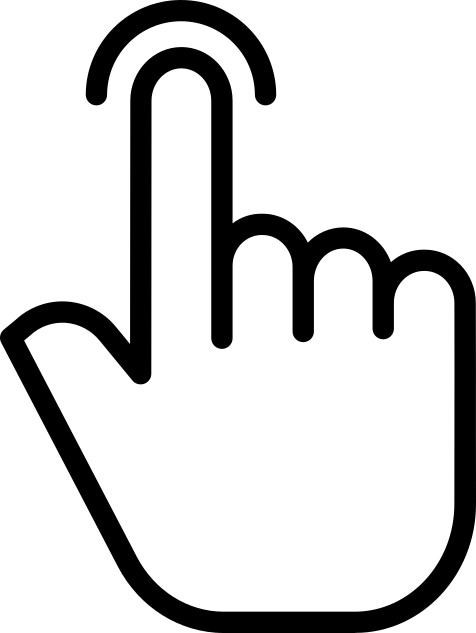
\includegraphics[width=0.10\textwidth]{static/dedo.png}} ;
    \node[const, left=of d] (nd) {\Large $s$};
    %\node[const, below=of d] (pd) {$\text{Creencia}(s=i|r=i, \text{Modelo}) = 0$}; 

    \edge {r} {d};
  }
  \caption{Modelo A}
  \label{fig:modelo_causal_1}
  \end{subfigure}
  \begin{subfigure}[b]{0.48\textwidth}
  \centering
  \tikz{        
    
    \node[latent] (d) {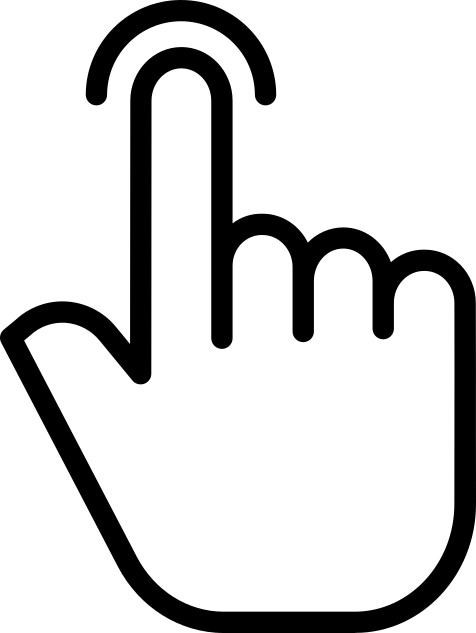
\includegraphics[width=0.10\textwidth]{static/dedo.png}} ;
    \node[const,above=of d] (nd) {\Large $s$} ;
    
    \node[latent, above=of d, xshift=-1.5cm] (r) {
\includegraphics[width=0.12\textwidth]{static/regalo.png}} ;
    \node[const,above=of r] (nr) {\Large $r$} ;
    
    \node[latent, fill=black!30, above=of d, xshift=1.5cm] (c) {
\includegraphics[width=0.12\textwidth]{static/cerradura.png}} ;
    \node[const,above=of c] (nc) {\Large $c=1$} ;
    
    \edge {r,c} {d};
  }
  \caption{Modelo B}
  \label{fig:modelo_causal_2}
  \end{subfigure}
  \caption{Modelos causales alternativos. Figura~\ref{fig:modelo_causal_1}: la pista s\'olo depende de la posici\'on del regalo. Figura~\ref{fig:modelo_causal_2}: la pista depende de la posici\'on del regalo y la la caja elegida previamente.
  Los c\'irculos representan las variables y la felcha representa la relaci\'on causa $\rightarrow$ efecto. 
  %A su vez, $r=i$ representa la proposici\'on ``el regalo se encuentra en la posici\'on $i$'', y $s=i$ representa la proposici\'on ``la pista se\~nala la posici\'on $i$''.
  }
  \label{fig:modelos_causales}
\end{figure}

% Parrafo
% %
% Por \'ultimo, lo que aparece del lado izquierdo del operador \emph{condicional} ($\cdot \mid \cdot$) son las proposiciones sobre las que computamos la creencia en los casos en los que las proposiciones que aparecen del lado derecha sean ciertas.
% %
% Es decir, la $\text{Creencia}(s=i|r=i,\text{Modelo}) = 0$ se lee como ``es imposible que la pista se\~nale la posici\'on $i$ cuando el regalo est\'a en la posici\'on $i$ y el modelo causal es cierto''. 
% 

% % Parrafo

Cada uno de los modelos causales alternativos tiene su propio conjuto finito de universos paralelos.
%
Siguiendo con el principio de indiferencia (o de m\'axima diversidad) dividimos la creencia en partes iguales en cada una de las bifurcaciones de los caminos paralelos del modelo causal.
%
En la figura~\ref{fig:caminos} mostramos c\'omo se dividen las creencias en partes iguales por los caminos paralelos de ambos modelos causales.

% Parrafo

En el modelo A, por cada posici\'on del regalo, se abren otros dos unviersos paralelos que se corresponden con las cajas hacia las que puede se\~nalar la pista, en las que no est\'a el regalo en ese universo.
%
En cambio, en el modelo B, la pista genera dos universos s\'olo cuando el regalo est\'a en la misma caja que elegimos, $r=1$.
%
% Podemos recibir una pista tanto en la puerta 2, $s_2$, como en la puerta 3, $s_3$.
% %
% Cuando el regalo est\'a en otra caja, $r\neq 1$, la pista puede se\~nalar \'unicamente a una de las cajas, la que no tiene el regalo y la que no fue elegida.
% %
% Por ejemplo, si el regalo est\'a en la puerta 2, $r_2$, la pista s\'olo puede se\~nalar la puerta 3, $s_3$.
%
\begin{figure}[H]
\centering
\begin{subfigure}[b]{0.48\textwidth}
\centering
\tikz{
\node[latent, draw=white, yshift=0.7cm] (b0) {$1$};

\node[latent,below=of b0,yshift=0.7cm, xshift=-2cm] (r1) {$r_1$};
\node[latent,below=of b0,yshift=0.7cm] (r2) {$r_2$};
\node[latent,below=of b0,yshift=0.7cm, xshift=2cm] (r3) {$r_3$};

\node[latent, below=of r1, draw=white, yshift=0.7cm] (br1) {$\frac{1}{3}$};
\node[latent, below=of r2, draw=white, yshift=0.7cm] (br2) {$\frac{1}{3}$};
\node[latent, below=of r3, draw=white, yshift=0.7cm] (br3) {$\frac{1}{3}$};
\node[latent,below=of br1,yshift=0.7cm, xshift=-0.5cm] (r1d2) {$s_2$};
\node[latent,below=of br1,yshift=0.7cm, xshift=0.5cm] (r1d3) {$s_3$};

\node[latent,below=of r1d2,yshift=0.7cm,draw=white] (br1d2) {$\frac{1}{3}\frac{1}{2}$};
\node[latent,below=of r1d3,yshift=0.7cm, draw=white] (br1d3) {$\frac{1}{3}\frac{1}{2}$};
\node[latent,below=of br2,yshift=0.7cm, xshift=-0.5cm] (r2d1) {$s_1$};
\node[latent,below=of br2,yshift=0.7cm, xshift=0.5cm] (r2d3) {$s_3$};
\node[latent,below=of br3,yshift=0.7cm, xshift=-0.5cm] (r3d1) {$s_1$};
\node[latent,below=of br3,yshift=0.7cm, xshift=0.5cm] (r3d2) {$s_2$};

\node[latent,below=of r2d1,yshift=0.7cm, draw=white] (br2d1) {$\frac{1}{3}\frac{1}{2}$};
\node[latent,below=of r2d3,yshift=0.7cm,draw=white] (br2d3) {$\frac{1}{3}\frac{1}{2}$};
\node[latent,below=of r3d1,yshift=0.7cm, draw=white] (br3d1) {$\frac{1}{3}\frac{1}{2}$};
\node[latent,below=of r3d2,yshift=0.7cm,draw=white] (br3d2) {$\frac{1}{3}\frac{1}{2}$};
\edge[-] {b0} {r1,r2,r3};
\edge[-] {r1} {br1};
\edge[-] {r2} {br2};
\edge[-] {r3} {br3};
\edge[-] {br1} {r1d2,r1d3};
\edge[-] {r1d2} {br1d2};
\edge[-] {r1d3} {br1d3};
\edge[-] {br2} {r2d1, r2d3};
\edge[-] {br3} {r3d1,r3d2};
\edge[-] {r2d1} {br2d1};
\edge[-] {r2d3} {br2d3};
\edge[-] {r3d1} {br3d1};
\edge[-] {r3d2} {br3d2};
}
\caption{Modelo A}
\label{fig:caminos_pre_montyhall}
\end{subfigure}
\begin{subfigure}[b]{0.48\textwidth}
\centering
\tikz{
\node[latent, draw=white, yshift=0.7cm] (b0) {$1$};
\node[latent,below=of b0,yshift=0.7cm, xshift=-2cm] (r1) {$r_1$};
\node[latent,below=of b0,yshift=0.7cm] (r2) {$r_2$};
\node[latent,below=of b0,yshift=0.7cm, xshift=2cm] (r3) {$r_3$};

% \node[latent, below=of r1, draw=white, yshift=0.8cm] (br1) {$\frac{1}{3}$};
% \node[latent, below=of r2, draw=white, yshift=0.8cm] (br2) {$\frac{1}{3}$};
% \node[latent, below=of r3, draw=white, yshift=0.8cm] (br3) {$\frac{1}{3}$};
% \node[latent,below=of br1,yshift=0.8cm] (c11) {$c_1$};
% \node[latent,below=of br2,yshift=0.8cm] (c12) {$c_1$};
% \node[latent,below=of br3,yshift=0.8cm] (c13) {$c_1$};

\node[latent, below=of r1, draw=white, yshift=0.7cm] (bc11) {$\frac{1}{3}$};
\node[latent, below=of r2, draw=white, yshift=0.7cm] (bc12) {$\frac{1}{3}$};
\node[latent, below=of r3, draw=white, yshift=0.7cm] (bc13) {$\frac{1}{3}$};
\node[latent,below=of bc11,yshift=0.7cm, xshift=-0.5cm] (r1d2) {$s_2$};
\node[latent,below=of bc11,yshift=0.7cm, xshift=0.5cm] (r1d3) {$s_3$};
\node[latent,below=of bc12,yshift=0.7cm] (r2d3) {$s_3$};
\node[latent,below=of bc13,yshift=0.7cm] (r3d2) {$s_2$};

\node[latent,below=of r1d2,yshift=0.7cm,draw=white] (br1d2) {$\frac{1}{3}\frac{1}{2}$};
\node[latent,below=of r1d3,yshift=0.7cm, draw=white] (br1d3) {$\frac{1}{3}\frac{1}{2}$};
\node[latent,below=of r2d3,yshift=0.7cm,draw=white] (br2d3) {$\frac{1}{3}$};
\node[latent,below=of r3d2,yshift=0.7cm,draw=white] (br3d2) {$\frac{1}{3}$};
\edge[-] {b0} {r1,r2,r3};
% \edge[-] {r1} {br1};
% \edge[-] {r2} {br2};
% \edge[-] {r3} {br3};
% \edge[-] {br1} {c11};
% \edge[-] {br2} {c12};
% \edge[-] {br3} {c13};
\edge[-] {r1} {bc11};
\edge[-] {r2} {bc12};
\edge[-] {r3} {bc13};
\edge[-] {bc11} {r1d2,r1d3};
\edge[-] {bc12} {r2d3};
\edge[-] {bc13} {r3d2};
\edge[-] {r1d2} {br1d2};
\edge[-] {r1d3} {br1d3};
\edge[-] {r2d3} {br2d3};
\edge[-] {r3d2} {br3d2};
}
\caption{Modelo B}
\label{fig:caminos_montyhall}
\end{subfigure}
\caption{Los caminos paralelos que se generan a partir de los modelos causales alternativos. El principio de m\'axima diversidad (o de indiferencia) divide la creencia en partes en cada una de las bifurcaciones de los caminos paralelos del modelo causal. }
\label{fig:caminos}
\end{figure}
%
Esto nos permite definir creencias honestas respecto de los universos paralelos. 
%
Cada camino del modelo causal tiene una combinaci\'on de valores distinta que representa nuestra \emph{creencia conjunta} honesta de que el regalo se encuentre en la caja $i$ y la pista se\~nale la caja $j$.
%
% Por ejemplo, la creencia conjunta de que el regalo est\'e en la caja $2$ y la pista se\~nale la caja $3$ es
% \begin{equation}
% \text{Creencia}(r=2 \wedge s=3 | \text{Modelo A} ) = \frac{1}{3} \frac{1}{2} = \frac{1}{6} \ \ \ \ \ \ \text{Creencia}(r=2 \wedge s=3 | \text{Modelo B} ) = \frac{1}{3} 
% \end{equation}
% %
% Donde $\wedge$ representa el conjunci\'on l\'ogica.
% %
% De aqu\'i en adelante remplazaremos este s\'imbolo por una simple coma ($,$).
% %
% Colocamos el modelo detr\'as del condicional ($\cdot|\cdot$) debido a que esta creencia conjunta es honesta cuando el modelo propuesto es cierto.
% %
% De aqu\'i en adelante s\'olo haremos expl\'icita la dependencia del modelo cuando haya alg\'un tipo de ambigüedad, que en general ocurre cuando hay m\'as de un modelo en disputa.
% %
% De la misma forma podemos calcular el resto de las creencias conjuntas a priori dado el modelo causal.
%
La conjunci\'on l\'ogica la expresamos con una simple coma ($,$), y colocamos del lado derecho del condicional ($\cdot|\cdot$) las proposiciones que momentanemante consideramos ciertas.
%
\begin{table}[H]
\centering
$P(r=i, s=j | \text{Modelo A})$ \hspace{1.8cm} $P(r=i, s=j | \text{Modelo B})$ \\[0.1cm]
 \begin{tabular}{|c|c|c|c|} \hline \setlength\tabcolsep{0.4cm}
       & \, $r_1$ \, &  \, $r_2$ \, & \, $r_3$ \, \\ \hline 
  $s_1$ & $0$ & $1/6$ & $1/6$  \\ \hline
  $s_2$ & $1/6$ & $0$ & $1/6$  \\ \hline
  $s_3$ & $1/6$ & $1/6$ & $0$ \\ \hline 
  \end{tabular}
  \hspace{1.5cm}
  \begin{tabular}{|c|c|c|c|} \hline  \setlength\tabcolsep{0.4cm} 
 & \, $r_1$ \, &  \, $r_2$ \, & \, $r_3$ \,  \\ \hline 
  $s_1$ & $0$ & $0$ & $0$ \\ \hline
  $s_2$ & $1/6$ & $0$ & $1/3$ \\ \hline
  $s_3$ & $1/6$ & $1/3$ & $0$  \\ \hline  
  \end{tabular}
  \caption{Creencia conjunta para cada uno de los modelos causales. El valor de las celdas representa la creencia honesta de cada uno de lsus caminos paralalelos. }
  \label{tab:creencia_conjunta}
\end{table}
%
Cada una de las celdas de la tabla representa una terminal de los caminos del modelo causal representados en la figura \ref{fig:caminos}.
% Parrafo
Tenemos entonces un principio para alcanzar acuerdos sobre las creencias conjuntas cuando la \'unica informaci\'on previa es el modelo causal multidimensional.

% Parrafo

Los caminos paralelos del modelo causal son hip\'otesis mutuamente excluytentes.
%
%Si ocurre uno de los caminos, no puede ocurrir el resto.
% 
% En ambos modelos, la pista se\~nala la caja $3$ cuando el regalo est\'a en la caja $1$ o en la caja $2$.
% Pero la creencia conjunta de esos caminos paralalelos es distinta.
% En el modelo A ambos caminos le asignamos una creencia de $1/6$, que sumadas representan $1/3$ de la creencia total.
% En el modelo B, en cambio, le asignamos una creencia de $1/6$ cuando el regalo est\'a en la caja $1$ y $1/3$ cuando el regalo est\'a en la caja $2$, que sumados represnetan $1/2$ del la creencia total.
% 
% % Parrafo
Habiendo definido la creencia conjunta sobre las hip\'otesis mutuamente excluyentes, por el principio de integridad podemos caclaular la creencia asignada a cada una de las variables individuales como una suma.
%
\begin{equation}
\begin{split}
P(s_j|\text{Modelo A}) = \sum_i P(r_i, s_j|\text{Modelo A}) = 1/3 \\  P(s_j|\text{Modelo B}) = \sum_i P(r_i, s_j|\text{Modelo B}) = 1/2
\end{split}
\end{equation}

% Parrafo

Lo mismo ocurre con cualquiera de las variables de un modelo multidimensional.
Para calcular la creencia sobre una variable, calculamos la suma de todos los caminos paralelos en los que esa variable est\'a presente.

\begin{table}[H]
\centering
Modelo A  \hspace{4.5cm}  Modelo B \\[0.1cm]
 \begin{tabular}{|c|c|c|c||c|} \hline \setlength\tabcolsep{0.4cm}
       & \, $r_1$ \, &  \, $r_2$ \, & \, $r_3$ \, & \\ \hline 
  $s_1$ & $0$ & $1/6$ & $1/6$ & $1/3$ \\ \hline
  $s_2$ & $1/6$ & $0$ & $1/6$ & $1/3$ \\ \hline
  $s_3$ & $1/6$ & $1/6$ & $0$ & $1/3$ \\ \hline \hline
   & $1/3$ & $1/3$ & $1/3$ & $1$ \\ \hline 
  \end{tabular}
  \hspace{1.5cm}
  \begin{tabular}{|c|c|c|c||c|} \hline  \setlength\tabcolsep{0.4cm} 
 & \, $r_1$ \, &  \, $r_2$ \, & \, $r_3$ \, & \\ \hline 
  $s_1$ & $0$ & $0$ & $0$ & $0$\\ \hline
  $s_2$ & $1/6$ & $0$ & $1/3$ & $1/2$ \\ \hline
  $s_3$ & $1/6$ & $1/3$ & $0$ & $1/2$ \\ \hline \hline
   & $1/3$ & $1/3$ & $1/3$ & $1$  \\ \hline
  \end{tabular}
  \caption{Creencia marginal obtenida como la suma de las creencia conjuntas honesta de cada uno de los caminos paralalelos de los modelos causales. }
  \label{tab:creencia_marginal}
\end{table}

En ambos modelos la creencia honesta sobre el regalos, sin importar el valor que toma pista, es $1/3$
\begin{figure}[H]
\centering
\tikz{ %
         \node[factor, minimum size=1cm] (p1) {
\includegraphics[width=0.025\textwidth]{static/cerradura.png}} ;
         \node[factor, minimum size=1cm, xshift=1.5cm] (p2) {} ;
         \node[factor, minimum size=1cm, xshift=3cm] (p3) {} ;

         \node[const, above=of p1, yshift=.15cm] (fp1) {$1/3$};
         \node[const, above=of p2, yshift=.15cm] (fp2) {$1/3$};
         \node[const, above=of p3, yshift=.15cm] (fp3) {$1/3$};
         \node[const, below=of p2, yshift=-.10cm, xshift=0.3cm] (dedo) {};
        } 
\caption{Creencia marginal sobre el regalo en ambos modelos causales. }
\end{figure}

\subsection{Principio de coherencia} \label{sec:principio_choerencia} % (dados los datos de base emp\'irica)

El principio de indiferencia nos permiti\'o definir la creencia conjunta honesta dividiendo las creencias en partes iguales por cada bifurcaci\'on del modelo causal.
%
Y el principio de integridad nos permiti\'o calcular la creencia honesta sobre una \'unica variable del modelo causal multidimensional como la creencia total de todos los caminos paralelos en los que esa variable est\'a presente.
%
¿Pero c\'omo para preservar los acuerdos intersubjetivos cuando recibimos nueva informaci\'on?
%
El principio de coherencia establece que la nueva creeencia honesta despu\'es de haber visto un nuevo datos es la creencia previa que sigue siendo compatible con ese dato.

% Parrafo

Supongamos que alguien nos indica con certeza que el regalo no est\'a en la caja del medio.
%
¿Cu\'al es la nueva creencia marginal honesta sobre el regalo despu\'es de haber visto esta pista?

% Parrafo

\begin{figure}[ht!]
\centering
\tikz{ %
        
         \node[factor, minimum size=1cm] (p1) {
\includegraphics[width=0.025\textwidth]{static/cerradura.png}} ;
         \node[det, minimum size=1cm, xshift=1.5cm] (p2) {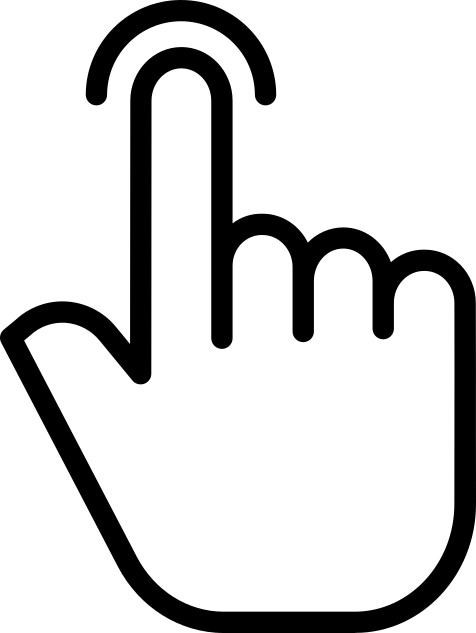
\includegraphics[width=0.03\textwidth]{static/dedo.png}} ;
         \node[factor, minimum size=1cm, xshift=3cm] (p3) {} ;
         \node[const, above=of p1, yshift=.15cm] (fp1) {$?$};
         \node[const, above=of p2, yshift=.15cm] (fp2) {$?$};
         \node[const, above=of p3, yshift=.15cm] (fp3) {$?$};
         \node[const, below=of p2, yshift=-.10cm, xshift=0.3cm] (dedo) {};
        
        } 
\end{figure}

% Parrafo

Para actualizar las creencias posiblemente nos veamos tentados a aplicar el principio de indiferencia nuevamente, asignando $0.5$ a las dos cajas que todav\'ia ocultan informaci\'on.
%
Aunque en este caso particular esa soluci\'on sea casualmente correcta para el modelo A, esa metodolog\'ia conduce a errores en t\'erminos generales.
%
El principio de indiferencia s\'olo se aplica una \'unica vez, al inicio.
%
Despu\'es s\'olo actualizaremos esa creencia en funci\'on de la nueva informaci\'on que vayamos incorporando.

Para ello revisemos cuales son los caminos paralelos del modelo causal que siguen siendo compatible con el observable.
%
Para actualizar las creencias simplemente nos quedamos con la creencia previa que es compatible con el dato, $P(r_i, s_2)$.
%
\begin{table}[ht!]
\centering
$P(r=i, s=2 | \text{Modelo A})$ \hspace{2.7cm} $P(r=i, s=2 | \text{Modelo B})$ \\[0.1cm]
\begin{tabular}{|c|c|c|c||c|} \hline \setlength\tabcolsep{0.4cm}
       & \, $r_1$ \, &  \, $r_2$ \, & \, $r_3$ \, & \\ \hline 
  $s_2$ & $1/6$ & $0$ & $1/6$ & $1/3$ \\ \hline
  \end{tabular}
  \hspace{1.5cm}
  \begin{tabular}{|c|c|c|c||c|} \hline  \setlength\tabcolsep{0.4cm} 
 & \, $r_1$ \, &  \, $r_2$ \, & \, $r_3$ \, & \\ \hline 
  $s_2$ & $1/6$ & $0$ & $1/3$ & $1/2$ \\ \hline
  \end{tabular}
  \caption{La creencia conjunta y marginal que sobrevive luego de ver los datos. }
  \label{tab:creencia_compatible}
\end{table}

En la tabla~\ref{tab:creencia_compatible} nos quedamos con la creencia conjunta y marginal que sigue siendo compatible con el dato.
%
Esto es exactamente lo mismo que quedarnos con los caminos del modelo causal que son posibles dado el modelo causal y el observable.
%
En la figura~\ref{fig:caminos_compatibles} mostramos los caminos que son compatibles en negro y los incompatibles en gris.

\begin{figure}[ht!]
\centering
\begin{subfigure}[b]{0.48\textwidth}
\centering
\tikz{
\node[latent, draw=white, yshift=0.7cm] (b0) {$1$};

\node[latent,below=of b0,yshift=0.7cm, xshift=-2cm] (r1) {$r_1$};
{\color{gray}\node[latent,draw=gray,below=of b0,yshift=0.7cm] (r2) {$r_2$};}
\node[latent,below=of b0,yshift=0.7cm, xshift=2cm] (r3) {$r_3$};

\node[latent, below=of r1, draw=white, yshift=0.7cm] (br1) {$\frac{1}{3}$};
{\color{gray}\node[latent, below=of r2, draw=white, yshift=0.7cm] (br2) {$\frac{1}{3}$};}
\node[latent, below=of r3, draw=white, yshift=0.7cm] (br3) {$\frac{1}{3}$};
\node[latent,below=of br1,yshift=0.7cm, xshift=-0.5cm] (r1d2) {$s_2$};
{\color{gray}\node[latent,draw=gray,below=of br1,yshift=0.7cm, xshift=0.5cm] (r1d3) {$s_3$};}

\node[latent,below=of r1d2,yshift=0.7cm,draw=white] (br1d2) {$\frac{1}{3}\frac{1}{2}$};
{\color{gray} \node[latent,draw=gray,below=of r1d3,yshift=0.7cm, draw=white] (br1d3) {$\frac{1}{3}\frac{1}{2}$}; }
{\color{gray}\node[latent,draw=gray,below=of br2,yshift=0.7cm, xshift=-0.5cm] (r2d1) {$s_1$}; }
{\color{gray} \node[latent,draw=gray,below=of br2,yshift=0.7cm, xshift=0.5cm] (r2d3) {$s_3$}; }
{\color{gray} \node[latent,draw=gray,below=of br3,yshift=0.7cm, xshift=-0.5cm] (r3d1) {$s_1$}; }
\node[latent,below=of br3,yshift=0.7cm, xshift=0.5cm] (r3d2) {$s_2$};

{\color{gray}\node[latent,below=of r2d1,yshift=0.7cm, draw=white] (br2d1) {$\frac{1}{3}\frac{1}{2}$};}
{\color{gray}\node[latent,below=of r2d3,yshift=0.7cm,draw=white] (br2d3) {$\frac{1}{3}\frac{1}{2}$};}
{\color{gray}\node[latent,below=of r3d1,yshift=0.7cm, draw=white] (br3d1) {$\frac{1}{3}\frac{1}{2}$};}
\node[latent,below=of r3d2,yshift=0.7cm,draw=white] (br3d2) {$\frac{1}{3}\frac{1}{2}$};
\edge[-] {b0} {r1,r3};
\edge[-,draw=gray] {b0} {r2};
\edge[-] {r1} {br1};
\edge[-,draw=gray] {r2} {br2};
\edge[-] {r3} {br3};
\edge[-] {br1} {r1d2};
\edge[-,draw=gray] {br1} {r1d3};
\edge[-] {r1d2} {br1d2};
\edge[-,draw=gray] {r1d3} {br1d3};
\edge[-, draw=gray] {br2} {r2d1, r2d3};
\edge[-] {br3} {r3d2};
\edge[-, draw=gray] {br3} {r3d1};
\edge[-, draw=gray] {r2d1} {br2d1};
\edge[-, draw=gray] {r2d3} {br2d3};
\edge[-, draw=gray] {r3d1} {br3d1};
\edge[-] {r3d2} {br3d2};
}
\caption{Modelo A}
\label{fig:caminos_pre_montyhall_compatibles}
\end{subfigure}
\begin{subfigure}[b]{0.48\textwidth}
\centering
\tikz{
\node[latent, draw=white, yshift=0.7cm] (b0) {$1$};
\node[latent,below=of b0,yshift=0.7cm, xshift=-2cm] (r1) {$r_1$};
{\color{gray}\node[latent,draw=gray,below=of b0,yshift=0.7cm] (r2) {$r_2$}; }
\node[latent,below=of b0,yshift=0.7cm, xshift=2cm] (r3) {$r_3$}; 

% \node[latent, below=of r1, draw=white, yshift=0.8cm] (br1) {$\frac{1}{3}$};
% \node[latent, below=of r2, draw=white, yshift=0.8cm] (br2) {$\frac{1}{3}$};
% \node[latent, below=of r3, draw=white, yshift=0.8cm] (br3) {$\frac{1}{3}$};
% \node[latent,below=of br1,yshift=0.8cm] (c11) {$c_1$};
% \node[latent,below=of br2,yshift=0.8cm] (c12) {$c_1$};
% \node[latent,below=of br3,yshift=0.8cm] (c13) {$c_1$};

\node[latent, below=of r1, draw=white, yshift=0.7cm] (bc11) {$\frac{1}{3}$};
{\color{gray}\node[latent, below=of r2, draw=white, yshift=0.7cm] (bc12) {$\frac{1}{3}$};}
\node[latent, below=of r3, draw=white, yshift=0.7cm] (bc13) {$\frac{1}{3}$};
\node[latent,below=of bc11,yshift=0.7cm, xshift=-0.5cm] (r1d2) {$s_2$};
{\color{gray}\node[latent,draw=gray,below=of bc11,yshift=0.7cm, xshift=0.5cm] (r1d3) {$s_3$};}
{\color{gray}\node[latent, draw=gray,below=of bc12,yshift=0.7cm] (r2d3) {$s_3$};}
\node[latent,below=of bc13,yshift=0.7cm] (r3d2) {$s_2$};

\node[latent,below=of r1d2,yshift=0.7cm,draw=white] (br1d2) {$\frac{1}{3}\frac{1}{2}$};
{\color{gray}\node[latent,below=of r1d3,yshift=0.7cm, draw=white] (br1d3) {$\frac{1}{3}\frac{1}{2}$};}
{\color{gray}\node[latent,below=of r2d3,yshift=0.7cm,draw=white] (br2d3) {$\frac{1}{3}$};}
\node[latent,below=of r3d2,yshift=0.7cm,draw=white] (br3d2) {$\frac{1}{3}$};
\edge[-] {b0} {r1,r3};
\edge[-,draw=gray] {b0} {r2};
% \edge[-] {r1} {br1};
% \edge[-] {r2} {br2};
% \edge[-] {r3} {br3};
% \edge[-] {br1} {c11};
% \edge[-] {br2} {c12};
% \edge[-] {br3} {c13};
\edge[-] {r1} {bc11};
\edge[-,draw=gray] {r2} {bc12};
\edge[-] {r3} {bc13};
\edge[-] {bc11} {r1d2};
\edge[-,draw=gray] {bc11} {r1d3};
\edge[-,draw=gray] {bc12} {r2d3};
\edge[-] {bc13} {r3d2};
\edge[-] {r1d2} {br1d2};
\edge[-,draw=gray] {r1d3} {br1d3};
\edge[-,draw=gray] {r2d3} {br2d3};
\edge[-] {r3d2} {br3d2};
}
\caption{Modelo B}
\label{fig:caminos_montyhall_compatibles}
\end{subfigure}
\caption{Los caminos paralelos compatibles (negro) e incompatibles (gris) con el dato $s=2$. }
\label{fig:caminos_compatibles}
\end{figure}
% Cuando aplicamos por primera vez el principio de indiferencia en la figura \ref{fig:principio_de_indiferencia}, el espacio de hip\'otesis se reduc\'ia a tres opciones, una por caja.
% %
% En este caso, en el que estamos considerando una variable nueva (la se\~nal $s$) que representa la pista, el espacio de hip\'otesis es otro, m\'as grande, por lo que esta creencia a priori no nos sirve.
% %

Es decir, para actualizar nuestra creencia nos quedamos con la creencia a priori que es compatible con los datos.
%
Lo que nos permitir\'a cumplir el objetivo que nos hab\'iamos propuesto, actualizar la creencia sobre el regalo luego de haber visto la pista.
%
\textbf{La creencia que sobrevive}, $P(r_i, s_2)$, es ahora nuestra nueva creencia total.
%
Para expresarla nuevamente como tal, la normalizamos para que vuelva a sumar 1.
%
\begin{equation}
P(r_i| s_2, \text{Modelo} ) = \frac{P(r_i, s_2| \text{Modelo})}{P(s_2| \text{Modelo})}
\end{equation}
%
La concusi\'on a la que llegamos depende del modelo causal elegido.
\begin{figure}[ht!]
\centering
\begin{subfigure}[b]{0.48\textwidth}
\centering
\tikz{ %
        
         \node[factor, minimum size=1cm] (p1) {
\includegraphics[width=0.05\textwidth]{static/cerradura.png}} ;
         \node[det, minimum size=1cm, xshift=1.5cm] (p2) {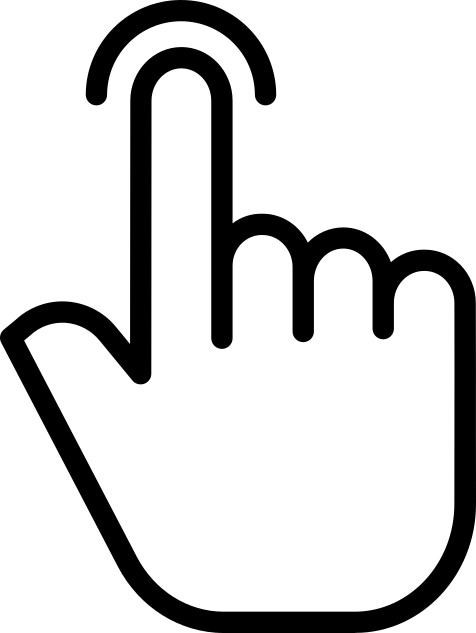
\includegraphics[width=0.06\textwidth]{static/dedo.png}} ;
         \node[factor, minimum size=1cm, xshift=3cm] (p3) {} ;

         \node[const, above=of p1, yshift=.15cm] (fp1) {$1/2$};
         \node[const, above=of p2, yshift=.15cm] (fp2) {$0$};
         \node[const, above=of p3, yshift=.15cm] (fp3) {$1/2$};
         \node[const, below=of p2, yshift=-.10cm, xshift=0.3cm] (dedo) {};
}
\caption{Modelos A}
\end{subfigure}
\begin{subfigure}[b]{0.48\textwidth}
\centering
\tikz{ %
        
         \node[factor, minimum size=1cm] (p1) {
\includegraphics[width=0.05\textwidth]{static/cerradura.png}} ;
         \node[det, minimum size=1cm, xshift=1.5cm] (p2) {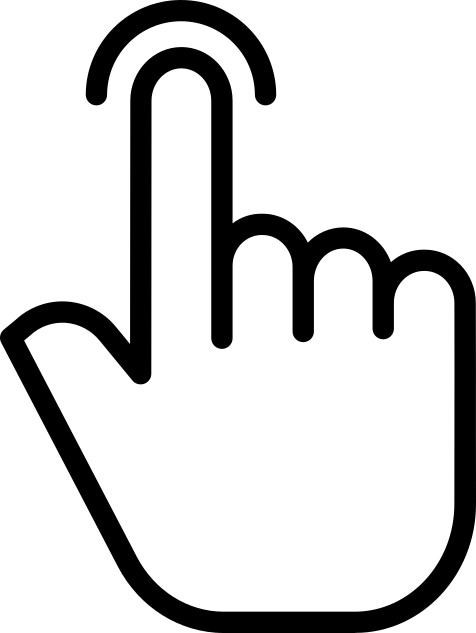
\includegraphics[width=0.06\textwidth]{static/dedo.png}} ;
         \node[factor, minimum size=1cm, xshift=3cm] (p3) {} ;
         
         \node[const, above=of p1, yshift=.15cm] (fp1) {$1/3$};
         \node[const, above=of p2, yshift=.15cm] (fp2) {$0$};
         \node[const, above=of p3, yshift=.15cm] (fp3) {$2/3$};
         \node[const, below=of p2, yshift=-.10cm, xshift=0.3cm] (dedo) {};
        }
\caption{Modelo B}
\end{subfigure}
\caption{Nueva creencia honesta dada el dato y el modelo}
\end{figure}
%  
Si bien ambas respuesta son diferentes, ambas comparten la propiedad de ser la distribuci\'on de creencias que maximiza la incertidumbre dada la evidencia formal (modelo causal) y emp\'irica (datos), lo que hace que sean proposiciones sobre las que podemos acordar tanto intercultural como intersubjetivamente.


\section{Las reglas de la probabilidad}\label{sec:reglas_de_la_probabilidad}

La teor\'ia de la probabilidad es actualmente el enfoque utilizado para representar incertidumbre asociada al conocimiento emp\'irico.
%
La teor\'ia de la probabilidad tiene puede resumirse en dos reglas, conocidas como la regla de la suma y la regla del producto.
%
La regla de la suma proviene del principio de integridad y establece que cualquier creencia marginal puede ser obtenida integrando la creencia conjunta.
%
\begin{equation}
P(r_i) = \sum_j P(r_i, s_j)
\end{equation}
%
La segunda regla proviene del principio de coherencia y, expresada como producto, establece que cualquier distribuci\'on conjunta puede ser expresada como el producto de distribuciones condicionales uni-dimensionles.
%
\begin{equation}
P(s_j)P(r_i|s_j) = P(r_i, s_j)
\end{equation}

% Parrafo

Las reglas de la probabilidad han sido derivadas formalmente a partir de una gran cantidad de sistemas axiom\'aticos conceptualmente distintos e independientes entre si, lo cual es uno de los puntos fuertes a su favor~\cite{halpern2017}.
%
El sistema axiom\'atico de Cox~\cite{cox} las deriva a partir de principios m\'as generales aun de los propuestos en la secci\'on anterior.
%
El sistema axiom\'atico de Ramsey~\cite{ramsey} las deriva haciendo una analog\'ia con los pagos que aceptar\'iamos en una apuesta, de forma similar a lo que veremos en la siguiente secci\'on. 
%
El sistema axiom\'atico de Kolmogorv~\cite{kolmogorov} tiene una motivaci\'on filos\'ofica menos expl\'icita, pero su simplicidad matem\'atica hace que sea el sistema axiom\'atico de referencia.
%
En el sistema de Kolmogorov la regla de la suma forma parte de los axiomas y la regla del producto de una definici\'on complementaria.
%
\begin{quotation}
Sea $E$ un conjunto de elementos $e_1, e_2, \dots$, y $F$ conjunto de subconjuntos de $E$.
%
\begin{enumerate}\itemsep-0.05cm
\item $F$ est\'a cerrada bajo complementos, uniones e intersecciones contables.
\item $F$ contiene al conjunto $E$
\item Todo conjunto $S \in F$ se le asigna una n\'umero real no negativo, $P(S)$.
\item $P(E) = 1$
\item Si $S_1, S_2, \dots$ son conjuntos mutuamente excluyente, luego
\begin{equation}
P(S_1 \cup S_2 \cup \dots ) = \sum P(S_i)
\end{equation}
\end{enumerate}
\end{quotation}
%
La regla de la suma se deriva inmediatamente del axioma 5 dado que siempre podemos expresar cualquier conjunto como $A = A \cap (B \cup \neg B)$.
%
La probabilidad condicional (o regla del producto) se incluye en el sistema como una definici\'on que cumple con los axiomas de la probabilidad. 

% %Ciertamentese ha dedicado mucho m\'as esfuerzo a justificar la teor\'ia de la probabilidad que cualquier otro enfoque para representar la incertidumbre y el tiempo dir\'a si se pueden se pueden desarrollar otros enfoques superadores.
% Pero quiz\'as m\'as importante es que su aplicaci\'on estricta (lo que llamamos inferencia Bayesiana) garantiza los acuerdos intersubjetivos a trav\'es de la maximizaci\'on de la incertidumbre (entrop\'ia) dada la informaci\'on emp\'irica y formal (datos y modelos causales)~\cite{Jaynes2003}.
% %

% Parrafo

As\'i expresada, la teor\'ia de la probabilidad est\'a basada en s\'olo dos de los cuatro principios vistos anteriormente, y carace de criterio para definir distribuciones de creencias iniciales (inferencia Bayesiana) y para expresar relaciones causales (inferencia causal).

\subsection{Teorema de Bayes}

El teorema de Bayes no es m\'as que un corolario de las reglas de las probabilidad, que surge de aplicar dos veces la regla del producto.
%
Usando las variables vistas en la secci\'on anterior, el teorema de Bayes puede expresarse como,
\begin{equation}
\begin{split}
P(r_i|s_2) = \frac{P(r_i, s_2)}{P(s_2)} = \frac{P(s_2|r_i)P(r_i)}{P(s_2)} 
\end{split}
\end{equation}
%
Es una pr\'actica muy com\'un no expresar expl\'icitamente que esas probabilidades en realidad dependen de un cierto modelo causal, por lo que lo correcto ser\'ia incluirlo en el condicional.
%
Notar adem\'as que escribimos a $r$ con un sub\'indice $i$ y a $s$ con un sub\'indice $2$.
%
Con esto queremos connotar la idea de que $r_i$ es una variable libre, que queremos evaluar para los diferentes valores (la hip\'otesis), y $s_2$ es un valor constante (el dato observado).
%
En l\'inea con esta interpretaci\'on, volvemos a expresar el teorema de Bayes de la siguiente manera.
% %
% \begin{equation*}
% \underbrace{P(\text{Hip\'otesis }|\text{ Datos})}_{\text{\scriptsize Posteriori}} = \frac{\overbrace{P(\text{Datos }|\text{ Hip\'otesis})}^{\text{\scriptsize Verosimilitud}} \overbrace{P(\text{Hip\'otesis})}^{\text{\scriptsize Priori}} }{\underbrace{P(\text{Datos})}_{\text{\scriptsize Evidencia}}}
% \end{equation*}
%
\begin{equation*}
\underbrace{P(\text{Hip\'otesis }|\text{ Datos, Modelo})}_{\text{\scriptsize Posterior}} = \frac{\overbrace{P(\text{Datos }|\text{ Hip\'otesis, Modelo})}^{\text{\scriptsize Verosimilitud}} \overbrace{P(\text{Hip\'otesis }|\text{ Modelo})}^{\text{\scriptsize Prior}} }{\underbrace{P(\text{Datos }|\text{ Modelo})}_{\text{\scriptsize Evidencia}}}
\end{equation*}
%
Los diferentes factores del teorema de Bayes han recibido nombres a lo largo de la historia, que revisemos a continuaci\'on.

\subsubsection*{Prior}

El \emph{prior} es la distribuci\'on de creencia inicial de las hip\'otesis dado el modelo causal antes de ver los datos.
%
En la secci\'on \emph{\nameref{sec:principio_indiferencia}} hemos visto un criterio intercultural que nos permite alcanzar un primer acuerdo intersubjetivo en contextos de incertidumbre.
%
El enfoque ``frecuentista'' de la teor\'ia de la probabilidad que rechaza todo criterio para definir distribuciones de creencias iniciales se ve impedido de utilizar el teorema de Bayes.
%
Como consecuencia, en vez de ofrecer distribuciones de probabilidad sobre todo el espacio de hip\'otesis, seleccionan una \'unica hip\'otesis (estimaci\'on puntual) en base a funciones de costo ad-hoc, siendo las m\'as com\'un la maximizaci\'on de la verosimilitud.

\subsubsection*{Verosimilitud}

La \emph{verosimilitud} es la predicci\'on del dato observado cuando suponemos que la hip\'otesis que estamos evaluando es cierta.
%
Veamos cu\'al es la verosimilitud, $P(s2|r_i, \text{Modelo B})$, la probabilidad de que la pista haya se\~nalado la caja $2$ en el modelo de Monty Hall para las diferentes posibles posiciones del regalo $r_i$.
%
\begin{figure}[ht!]
\begin{subfigure}[b]{0.7\textwidth}
\centering
\tikz{
\phantom{\node[latent, draw=white, yshift=0.8cm] (b0) {$1$};}
\node[latent,below=of b0,yshift=0.8cm, xshift=-2.5cm] (r1) {$r_1$};
\node[latent,below=of b0,yshift=0.8cm] (r2) {$r_2$};
\node[latent,below=of b0,yshift=0.8cm, xshift=1.8cm] (r3) {$r_3$};

\node[latent, below=of r1, draw=white, yshift=0.8cm] (br1) {$1$};
\node[latent, below=of r2, draw=white, yshift=0.8cm] (br2) {$1$};
\node[latent, below=of r3, draw=white, yshift=0.8cm] (br3) {$1$};

\node[latent,below=of br1,yshift=0.8cm, xshift=-0.7cm] (r1d2) {$s_2$};
\node[latent,below=of br1,yshift=0.8cm, xshift=0.7cm] (r1d3) {$s_3$};
\node[latent,below=of br2,yshift=0.8cm] (r2d3) {$s_3$};
\node[latent,below=of br3,yshift=0.8cm] (r3d2) {$s_2$};

\node[latent,below=of r1d2,yshift=0.8cm,draw=white] (br1d2) {$\frac{1}{2}$};
\node[latent,below=of r1d3,yshift=0.8cm, draw=white] (br1d3) {$\frac{1}{2}$};
\node[latent,below=of r2d3,yshift=0.8cm,draw=white] (br2d3) {$1$};
\node[latent,below=of r3d2,yshift=0.8cm,draw=white] (br3d2) {$1$};
\phantom{\edge[-] {b0} {r1,r2,r3};}
\edge[-] {r1} {br1};
\edge[-] {r2} {br2};
\edge[-] {r3} {br3};
\edge[-] {br1} {r1d2,r1d3};
\edge[-] {br2} {r2d3};
\edge[-] {br3} {r3d2};
\edge[-] {r1d2} {br1d2};
\edge[-] {r1d3} {br1d3};
\edge[-] {r2d3} {br2d3};
\edge[-] {r3d2} {br3d2};
}
\caption{Modelos causales B cuando conocemos la posici\'on del regalo.}
\end{subfigure}
\begin{subfigure}[b]{0.29\textwidth}
\centering
 $P(s_2|r_i,\text{Modelo B})$   
 
 \begin{tabular}{c|c|c|c} \setlength\tabcolsep{0.4cm} 
          & \, $r_1$ \, &  \, $r_2$ \, & \, $r_3$ \, \\ \hline 
   $s_2$ & $1/2$ & $0$ & $1$  \\ \hline
\end{tabular}
\vspace{1cm}
\caption{Verosimilitud}
\end{subfigure}   
\caption{Predicci\'on del dato observado dado que el modelo causal B y la hip\'otesis son ciertas. }
\end{figure}

%

Cuando el regalo est\'a en la misma posici\'on que la caja elegida $r=c=1$, el modelo causal permite que la pista se\~nale cualquiera de la otras dos cajas, por lo que la creencia a priori de que la caja se\~nalada sea la $s=2$ es $1/2$.
%
Cuando el regalo est\'a en una caja distinta a la elegida $r\neq c$, el modelo causal limita la pista a una \'unica caja.
%
Si el regalo est\'a en la caja $r=2$, la creencia a priori de que la caja se\~nalada sea la $s=2$ es $0$.
%
Y si el regalo est\'a en la caja $r=3$, la creencia a priori de que la caja se\~nalada sea la $s=2$ es $1$.

\subsubsection*{Posterior}

En la secci\'on \emph{\nameref{sec:principio_choerencia}} vimos que la nueva creencia no es m\'as que la creencia previa que sigue siendo compatible con el dato.
%
El teorema de Bayes nos permite ahora reconocer que la sorpresa que produce el dato observado es lo que act\'ua como filtro de las creencias previas.
%
Debido a que el denominador del teorema de Bayes es constante, la distribuci\'on de creencias a posteriori es proporcional al producto entre el prior y la verosimilitud.
%
\begin{table}[ht!]
\centering

$P(r_i|s_2, \text{M}_B) \propto P(r_i| \text{M}_B) P(s_2|r_i, \text{M}_B) $ \\[0.2cm]

\begin{tabular}{l|c|c|c} \setlength\tabcolsep{0.4cm} 
          & \, $r_1$ \, &  \, $r_2$ \, & \, $r_3$ \, \\ \hline 
   $P(s_2|r_i,\text{M}_B)$ & $1/2$ & $0$ & $1$  \\ \hline
   $P(r_i,\text{M}_B)$ & $1/3$ & $1/3$ & $1/3$  \\ \hline
   $P(r_i|s_2,\text{M}_B) \propto$ & $1/6$ & $0$ & $1/3$\\ \hline
\end{tabular}
\end{table}

% Parrafo

Como las verosimilitudes son predicciones, sus valores van entre $0$ y $1$.
%
Si la hip\'otesis $r=2$ fuera cierta, la sorpresa producida cuando observamos que la pista se\~nala la caja $s=2$ ser\'ia total.
%
En ese caso, como la predicci\'on del dato observado es $0$, nada del la creencia priori sobre $r=2$ pasa a la creencia a posteriori.
%
So la hip\'otesis $r=3$ fuera cierta, la sorpresa producida cuando observamos que la pista se\~nala la caja $s=2$ es nula.
%
En ese caso, como la predicci\'on del dato observado es $1$, toda la creencia priori sobre $r=2$ pasa a la creencia a posteriori.

% Parrafo

En inferencia Bayesiana entonces, la verosimilitud funciona como el filtro de las creencias previas. 

\subsubsection*{Evidencia}

De forma similar a la verosimilitud, la evidencia es una predicci\'on a priori del dato observado, pero que est\'a hecha con la contribuci\'on de todas las hip\'otesis.
%
Por la reglas de la probabilidad, el denominador del teorema de Bayes puede expresarse como una suma sobre todos los posibles valores del numerador, uno por cada hip\'otesis.
%
Esto hace que la evidencia sea constante para las diferentes hip\'otesis, por lo que puede ser ignorado cuando se comparan hip\'otesis alternativas.
%
Sin embargo, la evidencia va a ser distinta para los diferentes modelos.
%
En el modelo B la predicci\'on a priori de que la caja se\~nalada sea $s=2$, integrando todas las hip\'otesis, es $1/2$. 
%
\begin{equation}
P(s_2|M_B) = \sum_i P(s_2|r_i, M_B) P(r_i, M_B) = \frac{1}{2} \frac{1}{3} + 0 \frac{1}{3} + \frac{1}{1} \frac{1}{3} = 1/2 
\end{equation}
%
Mientras que en el modelo A la predicci\'on a priori de que la caja se\~nalada sea $s=2$, integrando todas las hip\'otesis, es $1/3$. 
%
\begin{equation}
P(s_2|M_A) = \sum_i P(s_2,r_i| M_A) = 1/3 
\end{equation}
%
Lo que ya hab\'ia sido calculado previamente en las marginales de la tabla \ref{tab:creencia_marginal}.

% Parrafo

La evidencia ser\'a de inter\'es cuando queramos evaluar modelos causales alternativos.
%
En la secci\'on \ref{sec:modelos_alternativos} mostramos en un ejemplo c\'omo deben evaluarse modelos causales alternativos aplicando estrictamente las reglas de la probabilidad.


\subsection{Las interpretaciones de la contradicción en la teoría probabilidad}
% 
% \subsection{La escuela naturalista (frecuentista)}
% 
% \subsection{La escuela epist\'emica (Bayesiana)}

Incluso las ciencias matem\'aticas, en contacto con problemas emp\'iricos, produjo diversas escuelas de pensamiento a pesar de estar regidas supuestamente bajo las mismas reglas te\'oricas.
%
La justificaci\'on axiom\'atica de la teor\'ia de la probabilidad no ha sido suficiente para unificar su interpretaci\'on.
%
El debate filos\'ofico de fondo respecto de las interpretaciones de la probabilidad tiene que ver con la soluci\'on que las dos principales escuelas le dieron al problema de la contradicci\'on: la solución epist\'emica (bayesiana) y la ontol\'ogica (frecuentista).

% Parrafo

En el siglo 18 el concepto de probabilidad comenz\'o a usarse en Europa para expresar creencias contradictorias en contextos de incertidumbre.
%
Por ejemplo, Laplace, qui\'en ten\'ia la convicci\'on de que el mundo era determinista, no pod\'ia m\'as que utilizar la probabilidad para expresar grados de creencia a hip\'otesis mutuamente contradictorias.
%
La estructura funcional de un mundo determinista impide por definición que A y no A ocurran dadas exactamente las mismas condiciones iniciales del mundo.
%
M\'as all\'a de la creencia particular de Laplace, bajo este marco la contradicci\'on de creer simultanemente en A y no A es s\'olo una expresi\'on de nuestra incertidumbre, y nada dice de la naturaleza (u ontolog\'ia) del mundo.

% Parrafo

La soluci\'on epist\'emica, que propon\'ia creer simultaneamente en hip\'otesis mutuamente contradictorias, fue el motivo por el cual la corriente bayesiana de la teor\'ia de la probabilidad fue tan combatida a finales del siglo 19 y durante casi todo el siglo 20.
%
A diferencia de las tradiciones filos\'oficas de origen oriental y americano, que ya admit\'ian alg\'un tipo de contradicci\'on en su sistema de creencias, la tradici\'on filos\'ofica Europea la rechazaba por completo.

% Parrafo

La escuela frecuentista, tal como se ense\~na en la materia probabilidad y estad\'isitica de la facultad de ciencias exactas y naturales, define a la probabilidad como el n\'umero al que tiende una frecuencia obtenida luego de realizar varios ``experimentos independientes'' bajo ``las mismas condiciones''.
%
Seg\'un esta corriente la probabilidad de eventos deterministas, por ejemplo de que exista un planeta no detectado en el sistema solar, es 0 o 1 aunque no conozcamos su valor.
%
S\'olo los objetos no deterministas, que llaman ``variables aleatorias'', pueden adquirir valores intermedios que representan la frecuencia en la que los diferentes estado del universo se producen a partir de exactamente las mismas condiciones inciales.
%
De esta forma, la contradicci\'on se propone como una propiedad externa al sistema l\'ogico, propia de la naturaleza del mundo.
%
La escuela frecuentista, para evitar la contradicci\'on en sus sistema l\'ogico, se ve obligada a afirmar la naturaleza aleatoria del mundo, lo que representa una la soluci\'on ont\'ol\'ogica de la contracci\'on.

\subsection{La funci\'on de costo epist\'emica}

% Lo que veremos en esta secci\'on es que la natrualeza multiplicativa de los procesos de selecci\'on evolutiva y probabilistica tiene una serie de propiedades que garantizan la adquisici\'on de conocimiento emp\'irico.
% 
% % Parrafo
Todas las axiomatizaciones alternativas de la teor\'ia de la probabilidad llegan a la conclusi\'on de que la forma natural de evaluar las hip\'otesis es a trav\'es de un proceso multiplicativo, la ``regla del producto''.
%
Por lo tanto, la \'unica función de costo habilitada para actualizar los recursos (probabilidades) de las distintas hipótesis es de naturaleza multiplicativa, como la analizada en el capítulo anterior.
%
Por el teorema de Bayes, la probabilidad de una hipótesis $h$ dado un conjunto de observables $\{d_1, \dots, d_n \}$ y un modelo causal $M$ es,
%
\begin{equation}
P(h|d_1, \dots, d_n, M) = \frac{P(d_1, \dots, d_n|h, M) P(h|M)}{P(d_1, \dots, d_n| M)} \propto \overbrace{P(d_1, \dots, d_n|h, M)}^{\text{Verosimilitud}} \overbrace{P(h|M)}^{\text{Prior}}
\end{equation}
%
La proporcionalidad vale debido a que el denominador es constante para las diferentes hipótesis.
%
Además, por la regla del producto la verosimilitud puede ser expresada como el producto de las predicciones a priori.
%
Luego, la probabilidad de una hipótesis a posteriori es proporcional a la probabilidad a priori multiplicada por las predicciones a priori de los datos observados.
%
\begin{equation}
P(h|d_1, \dots, d_n, M) \propto P(h|M) P(d_1|h,M) P(d_2|h,M,d_1) \dots
\end{equation}
%
La probabilidad puede ser vista como los recursos de cada una de las hipótesis tiene como el resultado de un juego de apuestas como los analizados en el capítulo anterior: el prior representa los recursos iniciales; las predicciones a priori son la apuesta, la asignación de recursos que hace cada una de las hipótesis antes de observar el dato ($b$ en la notación del capítulo anterior); y el pago de la casa de apuestas es nulo, $Q_{d_i} = 1$.  
%
En el cap\'itulo anterior hemos visto que los procesos multiplicativos siempre se maximiza dividiendo los recursos en la misma proproci\'on que la frecuencia t\'ipica $p$.
%
Gracias a la propiedad de los procesos multiplicativos, un juego de apuestas de este tipo garantiza que la hipótesis que asigna los recursos en la misma proporición que la frecuencia típica $p$ tiene la mayor tasa de crecimiento y por lo tanto se quedará con todos los recursos (probabilidad) a largo plazo. 
%
Es decir, a trav\'es de los resultados obtenidos en un juegos de apuestas podemos realizar ``inferencia'', descubrir la verdadera probabilidad a partir de la ignoracia, sin necesidad de que nadie conozca la probabilidad real.

% Parrafo

La interpretaci\'on ontol\'ogica de la teor\'ia de la probabilidad, al rechazar la contradicci\'on epist\'emica, se ve impedida de definir probabilidades iniciales (prior), y por lo tanto de utilizar el teorema de Bayes y resolver la inferencia usando el proceso multiplicativo como un juego de apuestas.
%
Como consecuencia, en vez de ofrecer distribuciones de probabilidad sobre todo el espacio de hip\'otesis, el enfoque frecuentista suele seleccionar una \'unica hip\'otesis (estimaci\'on puntual) en base a funciones de costo ad-hoc.
%
John Larry Kelly (Jr), quien trabajando con Shannon para los laboratorios Bell descubrió la propiedad epistémica de los procesos multiplicativos, comienza su art\'iculo ``A New Interpretation of Information Rate'' para los laboratorios Bell (1956) diciendo, 
%
\begin{quotation}
The author believes that [the cost function approach] it is too general to shed any light on the specific problems of communication theory. (...). The point here is that an arbitrary combination of a statistical transducer (i.e., a channel) and a cost function does not necessarily constitute a communication system. (...). The situation which will be chosen here is one in which a gambler uses knowledge of the received symbols of a communication channel in order to make profitable bets on the transmitted symbols.
\end{quotation}
%
En otras palabras, no toda funci\'on de costo garantiza la adquisici\'on de conocimiento emp\'irico.
%
El problema general del enfoque basado en funciones de costo ad-hoc tiene que ver con la influencia no deseada que decisiones arbitrarias tienen sobre las distribuci\'on de los recursos entre las hip\'otesis y por lo tanto sobre el resultado final de la inferencia.

% Parrafo

La funci\'on de costo m\'as utilizada por la corriente frecuentista es la maximizaci\'on de la verosimilitud.
%
Este enfoque a mostrado tener una serie de problemas siendo el m\'as conocido el problema del sobreajuste (u overfitting).
%
Para corregir este problema se han desarrollado otras funciones de costo ad-hoc que incluyen la penalizaci\'on por complejidad del modelo, y la separaci\'on de los datos con objetivos de ``entrenamiento'' y ``validaci\'on''.
%
A pesar de que estas metodolog\'ias se utilizan para entrenar redes neuronales modernas, ellas sufren en general de problemas de calibraci\'on: la predicción ofrecida por los modelos no se corresponde con la frecuencia observada.

% Parrafo

A diferencia del resto de las funciones de costo, los procesos multiplicativos tienen la propiedad especial de producir, no solo una distribuci\'on de recursos independiente de los pagos elegidos arbitrariamente, sino que garantiza adem\'as la hip\'otesis que apost\'o sus recursos en la misma proporci\'on que la frecuencia t\'ipica se quedar\'a en tiempo infinito con todos los recursos que ten\'ian las otras hip\'otesis.
%
En este sentido, los procesos multiplicativos jugados individualmente pueden ser vistos como la funci\'on de costo epistémica.

\subsection{Evaluación intersubjetiva de modelos causales}\label{sec:modelos_alternativos}

Los modelos causales tambi\'en son hip\'otesis, y por lo tanto, pueden ser evaluadas calculando su probabilidad dados los datos.
%
Usando el teorema de Bayes, la probabilidad de un modelo es
%
\begin{equation}\label{eq:p_modelo_|_datos}
 P(\text{Model\es{o}}|\text{Dat\en{a}\es{os}}) = \frac{\overbrace{P(\text{Dat\en{a}\es{os}}|\text{Model\es{o}})}^{\text{Evidencia}}P(\text{Model\es{o}})}{P(\text{Dat\en{a}\es{os}})}
\end{equation}
%
La verosimilitud de los modelos es lo que antes vimos como la evidencia, el denominador del posterior de las hip\'otesis de un modelo.
%
La evidencia es la predicci\'on a priori del dato observado con la contribuci\'on de todas las hip\'otesis.
%
Por la regla del producto, podemos expresar la evidencia como una productoria de predicciones a priori
%
\begin{equation}
\begin{split}
P(\text{Dat\en{a}\es{os}}|\text{Model\es{o}}) & = P(d_1|\text{Model\es{o}})P(d_2|d_1,\text{Model\es{o}}) \dots \\
& = \text{geometric mean}(P(\text{Dat\en{a}\es{os}}|\text{Model\es{o}}))^{|\text{Dat\en{a}\es{os}}|}
\end{split}
\end{equation}
%
La probabilidad conjunta de todos los datos dado el modelo es igual a la probabilidad del primer dato $d_1$ dado el modelo, por la probabilidad del segundo dato $d_2|d_1$ dado el primero y el modelo, y as\'i sucesivamente. 
%
La media geom\'etrica representa la predicci\'on ``t\'ipica''.
%
Notar que si alguna de las predicciones es $0$, toda la productoria se anula y la predicci\'on t\'ipica ser\'ia $0$.

% Parrafo

Esta naturaleza multiplicativa de los procesos de selecci\'on de los modelos hace que sea importante la reducci\'on de fluctuaciones.
%
Los modelos causales reducen fluctuaciones realizando las predicciones con la contribuci\'on de todas las hip\'otesis.
%
Por la regla de la suma, podemos expresar la evidencia como una suma de las predicciones conjuntas realizadas individualmente por cada una de sus hip\'otesis.
%
\begin{equation}
\begin{split}
P(\text{Dat\en{a}\es{os}}|\text{Model\es{o}}) & = \sum^{\text{Hip\'otesis}}_h P(\text{Dat\en{a}\es{os}}|h,\text{Model\es{o}}) P(h|\text{Model\es{o}}) \\
& = \text{arithmetic mean}_h(P(\text{Dat\en{a}\es{os}}|\text{Hip\'otesis},\text{Model\es{o}}))
\end{split}
\end{equation}
%
Notar que la media geom\'etica de la evidencia es igual a la media aritm\'etica de la contribuci\'on de todas las hip\'otesis.
%
Con que una \'unica hip\'otesis asigne a los datos probabilidad mayor a $0$, la evidencia tambi\'en ser\'a mayor a $0$, evitando as\'i el peor caso.
%
De esta forma, las hip\'otesis de un mismo modelo cooperan en la predicci\'on a priori de los datos observados, evitando los problemas de sobreajuste asociados a los enfoque frecuentista que seleccionan una \'unica hip\'otesis del espacio.
%
Combinando la regla del producto y de la suma podemos expresar la evidencia como una productoria de sumatorias.
%
 \begin{equation}
\begin{split}
P(\text{Dat\en{a}\es{os}}|\text{Model\es{o}}) & = P(d_1|\text{Model\es{o}})P(d_2|d_1,\text{Model\es{o}}) \dots \\
& = \left( \sum^{\text{Hipo}}_h P(d_1|h,\text{M}) P(h|\text{M}) \right) \left( \sum^{\text{Hipo}}_h P(d_2|d_1,h,\text{M}) P(h|d_1,\text{M}) \right)  \dots \\\end{split}
\end{equation}
%
Cada predicci\'on individual de la productoria es una en el fondo una media aritm\'etica.
%
As\'i, el modelo reduce fluctuaciones en cada una de las predicciones individuales a trav\'es de la contribuci\'on que realiza el conjunto de sus hip\'otesis.

% Parrafo

El denominador de la ecuaci\'on \ref{eq:p_modelo_|_datos} es la predicci\'on a priori del dato observado con la contribuci\'on de todos los modelos (y todas sus hip\'otesis).
%
Cuando no conocemos el espacio completo de modelos alternativos, no vamos a poder computar la probabilidad de ning\'un modelo.
%
Pero al menos, vamos a poder comparar la probabilidad relativa entre modelos.
%
 \begin{equation}
\begin{split}
 \frac{P(\text{Modelo A}|\text{Datos})}{P(\text{Modelo B}|\text{Datos})} = \frac{P(\text{Data}|\text{Modelo A})\cancel{P(\text{Modelo A})}}{P(\text{Data}|\text{Modelo B})\cancel{P(\text{Modelo B })}}
\end{split}
\end{equation}
%
Cuando el prior de ambos modelos es igual, la probabilidad relativa entre modelos depende de sus predicciones a priori.
%
A esta expresi\'on se la conoce como Bayes Factor.
%
Para preferir un modelo sobre otro es importante que la diferencia relativa sea de varios \'ordenes de magnitud.
%
En general es preferible expresarla en escala logar\'itimica porque hace que esta expresi\'on se vuelva sim\'etrica (qui\'en est\'a en el numerador y en el denominador solo modifica el signo) y porque expresa la diferencia en \'ordenes de magnitud.

% Parrafo

En el siguiente ejemplo haremos selecci\'on de los modelos vistos al inicio de este cap\'itulo.
%
Supongamos que los datos se generan siguiendo el modelo causal Monty Hall, 32 veces.
%
Alrededor de una de cada tres veces el regalo estar\'a escondido detr\'as de la caja 1, $r=1$.
%
\begin{lstlisting}[backgroundcolor=\color{all}]
regaloEn1 = [ rand(1:3) == 1 ? 1 : 0 for _ in 1:32]
\end{lstlisting} 
%
Supongamos que siempre elegimos la caja 1, $c=1$.
%
Seg\'un el modelo Monty Hall la pista s\'olo se\~nalara a la caja 2 o la caja 3, $s \in \{2,3\}$.
%
Los datos que vamos a mostrarle a los modelos son primero la pista, y despu\'es la posici\'on real del regalo.
%
La evidencia (predicci\'on a priori) de cada una de las pistas individuales va a ser $1/3$ para el modelo A y $1/2$ para el modelo B.
%
Y evidencia (predicci\'on a priori) de cada una de las posiciones de individuales de los regalos va a ser $1/2$ para el modelo A y para el modelo B va a ser $1/3$ cuando el regalo est\'e en la caja 1 y $2/3$ cuando est\'e en otra.
%
\begin{lstlisting}[backgroundcolor=\color{all}]
evidencia_A = cumprod([(1/3)*(1/2) for _ in regaloEn1])
evidencia_B = cumprod([(1/2)*( (1/3)^(r1)*(2/3)^(1-r1) ) for r1 in regaloEn1])
\end{lstlisting} 
%
Tomamos la productoria acumulada para mostrar gr\'aficamente c\'omo se actualizan las probabilidades a medida que observamos datos nuevos (Figura~\ref{fig:modelos_alternativos}).
%
Considerndo priors iguales, la probabilidad de los modelos es,
%
\begin{lstlisting}[backgroundcolor=\color{all}]
prior = 1/2
p_datos = (evidencia_A .* prior) .+ (evidencia_B .* prior)
p_modelo_A = evidencia_A .* prior ./ p_datos
p_modelo_B = evidencia_B .* prior ./ p_datos
\end{lstlisting} 
%
R\'apidamente, con menos de 32 observaciones, es casi seguro que el modelo causal B es el que representa el que mejor captura el comportamiento de la naturaleza.
%
\begin{figure}[H]
    \centering
    \begin{subfigure}[b]{0.5\textwidth}
    \includegraphics[width=\linewidth]{figures/monty_hall_selection.pdf}
    \end{subfigure}
    \caption{
    Selecci\'on de modelos alternativos
    }
    \label{fig:estrategias_individuales}
\end{figure}
%
Este mismo m\'etodo ser\'a usado en para evaluar el modelo de estimaci\'on de habilidad que utilizaremos para analizar datos de comunidades virtuales.

\section{Construcci\'on de datos de base empírica} \label{sec:base_empirica_metodo}

La ciencia, como proyecto de construcción de conocimiento universalizable, nos obliga a poner en correspondencia unívoca los fenómenos percibidos por nuestras conciencias con alg\'un esquema de operación que sea p\'ublicamente inteligible y reproducible.

\subsection{Base empírica y datos T-teóricos}

Llamamos \emph{base empírica} a la porción del ``mundo'' que es aceptada  como verdad por una comunidad, al menos por un cierto momento.
%
Para aceptar la entidad de nuestros objetos m\'as cotidianos, como por ejemplo el precio al que ayer nos vendieron los tomates en la verduler\'ia, o el resultado de la final de los \'ultimos mundiales de f\'utbol, son suficientes los supuestos del sentido com\'un.
%
A pesar de que existan círculos filosóficos que pretendan poner en duda las percepciones y supuestos más básicos, reduciendo la base empírica a un conjunto vacío (base empírica \emph{filosófica}), en la vida cotidinana no hay mayor controversia al respecto.
%
Los objetos que cualquier persona tomaría por ciertos en su vida cotidiana constituyen una base empírica significativamente más amplia, que Klimovsky llama base empírica \emph{epistemológica}, pues son la base inicial de toda actividad científica normal.
%
Sin embargo, a medida que la ciencia y la técnica se desarrollan, nuevos objetos construidos a partir de hipótesis o teorías comienzan a tener una aceptación general debido a que esos nuevos supuestos dejan de estar en duda al interior de cierta comunidad científica.
%
El conjunto de objetos que incluye aquellos objetos derivados de los nuevos acuerdos científicos se lo conoce como base empírica \emph{metodológica}~\cite{klimovsky1994-desventuras}.

% Parrafo

Es cualquier caso, todos los datos est\'an cargados de hip\'otesis.
%
Visto de esta manera, la base empírica depende del conjunto de supuestos que una comunidad esté dispuesta a admitir sin poner en duda.
%
Las diferentes niveles de bases empíricas formarían una estructura en ``capas de cebolla'', con un n\'ucleo de base empírica epistemológica y capas sucesivas $i$ de bases empíricas metodológicas, BEM$_i$. 
%
Para que ellos puedan actuar como base emp\'irica sobre la que se eval\'uan las teor\'ias cient\'ificas es necesario que sus supuestos queden, al menos por un cierto momento, fuera de toda duda.
%
\begin{figure}[ht!]
    \centering
    \begin{subfigure}[b]{0.48\textwidth}
    \includegraphics[page=4,width=\linewidth]{figures/baseEmpirica.pdf}
    \end{subfigure}
    \caption{Niveles de base emp\'irica. En negro la base emp\'irica epistemol\'ogica, en gris las bases emp\'iricas metodol\'ogicas, y en blanco los datos que todav\'ia no han alcanzado un acuerdo intersubjetivo amplio, que dependen de la aceptación de una nueva teoría T. }
\end{figure}

% Parrafo

Si los datos son una construcción teórica entonces, concluyen los críticos, la actividad pierde todo control externo y la ciencia no sería más que un juego de autojustificación.
%
Sin embargo, es el concepto mismo de base empírica como construcción relativa a supuestos lo que permite superar esa crítica pertinente.
%
La actividad científica mantiene su control externo en tanto existe siempre un conjunto de datos que si bien están cargados de supuestos, no lo están de los supuestos de la teoría para los que son datos. En palabras de Díez y Lorenzano~\cite{lorenzano2002-concepcionEstructuralista},
%
\begin{quotation}
Un término, un concepto, o una entidad, no es teórico o no teórico sin más, sino relativamente a una teoría dada.
Por eso no se debe hablar tanto de teoricidad cuanto de T-teoricidad, teoricidad relativa a la teoría T. (...).
La idea es que un concepto es T-teórico si no se puede determinar sin presuponer la aplicabilidad de T, si todo procedimiento para su determinación la presupone; y puede obtenerse sin presuponer tal teoría, si tiene alg\'un procedimiento de determinación T-independiente, por más que también tenga otros T-dependientes.
\end{quotation}
%
Los datos T-no teóricos son la base empírica de control para una teoría T pues pueden ser construidos mediante teorías independientes, previamente aceptadas.
%
En la secci\'on ``\nameref{sec:modelos_alternativos}'' hemos visto c\'omo garantizar los acuerdos intersubjetivos en la evaluación de los modelos causales alternativos.
%
En el cap\'itulo \ref{ch:ttt} seleccionamos el modelo de estimaci\'on de habilidad estado-del-arte en la industria del video juego, conocido como TrueSkill Through Time (TTT).

\subsection{Estructura invariante y operacionalización del dato empírico}

Los datos científicos tienen una estructura funcional, $f(x)=y$, donde la $x$ representa la unidad de análisis, las $f$ la variable, y la $y$ el resultado.
%
La estructura funcional de las proposiciones empíricas obliga que se cumpla la propiedad de replicabilidad: cada vez que se vuelve a medir la misma variable sobre la misma unidad de análisis debemos obtener el mismo resultado\footnote{Además de la unidad de análisis, otros parámetros de contexto pueden ser necesarios para que se cumpla esta propiedad funcional, los cuales sin pérdida de generalidad serán omitidos en esta sección, a pesar de que serán cosiderados cuando resolvamos los problemas reales en los siguientes capítulos.}.
%
Al conversar informalmente usamos estas estructuras funcionales para expresar, por ejemplo, que la habilidad de Maradona fue superior a la de Messi.
%
\begin{equation}\label{eq:opiniones}
 \emph{Habilidad}(\text{Maradona}) > \emph{Habilidad}(\text{Messi})
\end{equation}
%
En este caso, la funci\'on \emph{Habilidad} representa una cierta variable o caracter\'istica, que aplicada sobre una unidad de an\'alisis particular, Messi o Maradona, debe devolver siempre el mismo resultado.
%
Sin embargo, cuando conversamos hablamos en términos abstractos y no hacemos explícita la definici\'on precisa de la funci\'on, por lo que dos personas pueden usar la misma palabra para expresar conceptos que en el fondo son distintos.
%
Ahí radica el origen de muchos de los desacuerdos que se producen en ciencia y en la vida cotidiana.
%
El significado preciso del dato depende de su ``operacionalizaci\'on'', del procedimiento de determinación, que transforma la aplicación de la función en su resultado.
%
Allí donde identificamos, en la sección anterior, el lugar que debemos conocer en detalle para saber respecto de qué teorías T depende el dato, y por lo tanto su nivel de base empírica metodológica.

% Parrafo

La estructura funcional $f(x)=y$ es la parte más abstracta del dato, su parte formal.
%
Esto permite que los modelos de simulación, que no tienen contacto alguno con datos reales, puedan hablar del comportamiento de los datosjustamente gracias a que existe esta estructura superior puramente abstracta.
%
Sin embargo, los dato empíricos tiene una subestructura invariante que justifica los valores absrrtactos a través de la praxis: el esquema indicidor.
%
Debemos esta propuesta al epistemólogo Argentino, contemporáneo de Gregorio Klimovsky y Rolando García, el profesor Juan Samaja.
%
Seg\'un la hipótesis de Samaja~\cite{samaja} (que él desafía a que encuentren un contra-ejemplo), todo esquema indicador se compone de dimensiones (D), que son especificaciones de la variable (V), y de procedimientos (P) protocolos, acciones que efectuadas sobre cierta fuente de datos (F) producen señales o indicadores (I), objetos perceptibles desde el sentido com\'un, que interpretados con alguna hipótesis indicadora definen los resultados (R).
%
\begin{table}[ht!]
\centering \footnotesize
\begin{tabular}{cccc}
$f$ & \normalsize $x$ &\normalsize  = & $y$    \\ 
  \normalsize  Variable (V) & \normalsize  Unidad de An\'alisis (UA) &\normalsize   &\normalsize  Resultado (R)    \\ \hline
 $\downarrow$ &$\downarrow$&&$\uparrow$ \\
 Examen de representatividad &Examen de viabilidad & & Hipótesis indicadora \\
 $\downarrow$ &$\downarrow$&&$\uparrow$ \\
 \normalsize Dimensiones (D) & \normalsize Fuente de datos (F) &  & \normalsize Indicador (I) \\
 $\downarrow$ &$\downarrow$&&$\uparrow$ \\
 \multicolumn{2}{c}{Examen de confiabilidad} & & Sentido com\'un \\
 \multicolumn{2}{c}{$\downarrow$} & &$\uparrow$ \\
 \multicolumn{2}{c}{\normalsize Procedimiento (P)} & $\rightarrow$ & \normalsize Percepción \\
\end{tabular}
\caption{Estructura invariante del todo dato emp\'irico propuesta por Juan Samaja.}
\label{tab:matriz_datos}
\end{table}
%
El contenido de cada uno de sus elementos depende de una serie de supuestos.

% Parrafo

La selección de las dimensiones (D) depende de que estas expresen el concepto de la variable a través de alg\'un modelo causal en el que exista con la variable (V) una relación, directa o indirecta, que permitia eventualmente realizar un flujo de inferencia entre ellas, actualizando así la distribución de creencias sobre el valor de la variable (R) una vez que todas las dimensiones elegidas hayan sido observadas.
%
A esta estapa se la conoce como examen de \emph{representatividad}.
%
Por ejemplo, si la variable es la \emph{Habilidad$(\cdot)$}, una dimensión posible a ser observada, especifica el concepto de la variable, son los resultados de los eventos deportivos (ganar/perder), pues en cualquier modelo causal que elijamos existirá un relación, directa o indirecta, entre ellas.
%
Durante la selección de la fuente de datos (F), el examen de \emph{viabilidad}, se eval\'ua la autenticidad y accesibilidad de la informaci\'on.
%
Por ejemplo, podemos utilizar la p\'agina oficial de la asociaci\'on de tenis profesional ATP, \texttt{atptout.com} como fuente de datos.
%
La definici\'on de los protocolos (P), el examen de \emph{confiabilidad}, se eval\'ua que los procedimientos detecten s\'olo esa dimensi\'on de la fuente y no otros est\'imulos asociados, y de discriminar m\'inimas cantidades.
%
Por ejemplo, un \emph{scraper} nos permite extraer de forma segura los resultados de las partidas de la página oficial, generenado en cada caso un indicador binario (verdadero/falso) que se obtiene desde el sentido com\'un.
%
\begin{itemize} \itemsep-0.05cm
\item[$\bullet$] Dimensiones (D): Ganar/Perder
\item[$\bullet$] Fuente de datos (F): \texttt{atptour.com}
\item[$\bullet$] Procedimiento (P): Scraper
\item[$\bullet$] Indicador (I): True/False
\end{itemize}
%
Ahora bien, ¿c\'omo hacemos para pasar del indicador al resultado?.
%
Para ello necesitamos determinar cual es la hip\'otesis indicadora.
%
En la siguiente sección veremos una hipótesis indicadora ad-hoc que ha sido muy efectiva y sigue siendo utilizada por la federación internacional de ajedrez para determinar la habilidad de los ajedrecistas profesionales.
%
Y en la subsiguiente sección veremos que existe una hip\'otesis indicadora general que nos permite incorporar informaci\'on de los observables en nuestras distribuciones de creencia garantizando los acuerdos intersubjetivos.

\subsection{Una hipótesis indiciadora ad-hoc exitosa}

La hipótesis indicadora propuesta por Elo para estimar la habilidad de los ajedrecistas profesionales está basada en un modelo causal determinista con incertidumbre, en el que las habilidades generan el resultado observado a través de desempeños aleatorios (figura~\ref{fig:modelo_Elo}).
%
\begin{figure}[ht!]\centering
\begin{subfigure}[c]{0.49\textwidth}
\centering \small
    \tikz{         
    \node[det, fill=black!10] (r) {$r$} ; 
    \node[const, left=of r, xshift=-1.35cm] (r_name) {\small \en{Result}\es{Resultado}:}; 
    \node[const, right=of r] (dr) {\normalsize $ r = (d > 0)$}; 

    \node[latent, above=of r, yshift=-0.45cm] (d) {$d$} ; %
    \node[const, right=of d] (dd) {\normalsize $ d = p_i-p_j$}; 
    \node[const, left=of d, xshift=-1.35cm] (d_name) {\small \en{Difference}\es{Diferencia}:};
    
    \node[latent, above=of d, xshift=-0.8cm, yshift=-0.45cm] (p1) {$p_i$} ; %
    \node[latent, above=of d, xshift=0.8cm, yshift=-0.45cm] (p2) {$p_j$} ; %
    \node[const, left=of p1, xshift=-0.55cm] (p_name) {\small \en{Performance}\es{Desempe\~no}:}; 

    \node[accion, above=of p1,yshift=0.3cm] (s1) {} ; %
    \node[const, right=of s1] (ds1) {$s_i$};
    \node[accion, above=of p2,yshift=0.3cm] (s2) {} ; %
    \node[const, right=of s2] (ds2) {$s_j$};
    
    \node[const, right=of p2] (dp2) {\normalsize $p \sim \N(s,\beta^2)$};

    \node[const, left=of s1, xshift=-.85cm] (s_name) {\small \en{Skill}\es{Habilidad}:}; 
    
    \edge {d} {r};
    \edge {p1,p2} {d};
    \edge {s1} {p1};
    \edge {s2} {p2};
   
}
\caption{Modelo causal}
\end{subfigure}
   \begin{subfigure}[c]{0.49\textwidth}
       \includegraphics[width=0.8\textwidth]{figures/probaOfWin_2D.pdf} 
     \caption{Probabilidad de ganar}
     \label{fig:probaOfWin_2D}
    \end{subfigure}
     \caption{
     \es{Modelo en el que las habilidades causan los resultados observables a trav\'es de la diferencia de rendimientos ocultos, $d=p_i-p_j$, ambas variables aleatorias centradas en la verdadera habilidad, $p \sim \N(s,\beta^2)$. }%
    %
    \es{Quien haya obtenido mayor rendimiento gana, $r = (d > 0)$. }%
    \es{Las variables observables se pintan de gris, las ocultas en blanco, y las constantes se muestran como puntos negros. }%
    }
    \label{fig:modelo_Elo}
\end{figure}
%
Los agentes exhiben distintos desempe\~nos en cada evento, que var\'ian alrededor de su verdadera habilidad, $\N(p\,|\,s,\beta^2)$.
%
El modelo supone que gana el agente con mayor rendimiento, $r = (p_i > p_j)$.
%
En otras palabras, gana quien obtenga una diferencia de desempe\~no mayor a 0, $r = (p_i - p_j > 0)$.
%
A partir de este modelo causal podemos derivar la probabilidad de ganar a priori, $P(r|s_i^{\text{old}},s_j^{\text{old}})$, que en términos gráficos es equivalemte al volumen indicado en la figura \ref{fig:probaOfWin_2D}.
%
El complemento de la predicción lo vamos a llamar sorpresa.
%
\begin{equation*}
 \Delta = \underbrace{(1 - P(r|s_i^{\text{old}},s_j^{\text{old}}))}_{\hfrac{\textbf{Sorpresa}}{\text{del resultado}}}
\end{equation*}
%
La idea es que la magnitud de la sorpresa $\Delta$ est\'a relacionada con cuan buenas son las estimaciones previas, y por lo tanto puede usarse para actualizarlas.
%
Resultados inesperados indicar\'ian que las estimaciones actuales no son del todo correctas y deber\'ian actualizarse en mayor medida que si hubieran ocurrido como se esperaba.
%
La propuesta de Elo fue entonces utilizar la sorpresa como factor de corrección de las estimaciones previas.
%
\begin{equation}\label{eq:elo_update}
 s_{\text{winner}_\text{new}} = s_{\text{winner}_\text{old}} + \Delta \ \ \ \ \ s_{\text{loser}_\text{new}} = s_{\text{loser}_\text{old}} - \Delta 
\end{equation}
%
Esta es la hip\'otesis indicadora de Elo.
%
Esta soluci\'on es capaz de recuperar la escala relativa de los agentes, partiendo de valores iniciales arbitrarios.
%
\begin{center}
\tikz{ %
        \node[const] (e) {Estimaci\'on}; 

        \node[const, xshift=3cm] (p) {Predicci\'on};
        \node[const, xshift=1.5cm, yshift=-1cm] (s) {Sorpresa}; 
        
         \edge {e} {p};
         \edge {p} {s};
         \edge {s} {e};
} 
\end{center}
%
Esta definci\'on de habilidad es usada todav\'ia hoy por la federaci\'on internacional de ajedrez (FIDE).
%
Sin embargo, el sistema Elo tiene algunas debilidades importantes.
%
La regla de actualizaci\'on (Ec.~\eqref{eq:elo_update}) es sim\'etrica, as\'i que lo que gana un agente el otro lo pierde.
%
Debido a que a los agentes nuevos comienzan con estimaciones arbitrarias (el mismo valor inicial para cualquier individuo), ellas tienden a generan alta sorpresa y por lo tanto pueden modificar bruscamente las estimaciones de sus oponentes a pesar de que ya hubieran convergido.
%
Esta debilidad ocurre por no tener en cuenta la incertidumbre sobre las estimaciones de los agentes.
%
Para resolver este problema se propuso reducir el impacto de la sorpresa en funci\'on de la cantidad de veces que el agente ha participado previamente.
%
Ese es rol que desempe\~na el K-factor usado por la FIDE, $\Delta_i = \Delta \cdot K_i$.
%
A medida que la persona tiene más cantidad de partidas jugadas, el valor de K es menor.
%
De esa forma se rompe la simetría y se preserva las estimaciones de las personas que se consideran conocidas.


\subsection{La hipótesis indiciadora universal}

Los problemas asociados al algoritmo Elo se generan debido a que la hipótesis indicadora utilizada no esta justificada correctamente.
%
En este capítulo hemos introducido los principios interculturales de acuerdos intersubjetivos a partir de los que derivamos las reglas de la probabilidad.
%
Por ello, para corregir los problemas del algoritmo Elo, en vez de seleccionar una \'unica hipótesis de habilidad (estimación puntual), debemos aplicar estrictamente las reglas de la probabilidad y calcular la distribución de creencia sobre todo el espacio de hipótesis.
%
El teorema de Bayes, que se deriva de las reglas de la probabilidad, es en este sentido la hipótesis indicadora general, la que permite actualizar la distribución de creencia a priori de forma óptima.
%
En nuestro caso particular, debemos computar la probabilidad hip\'otesis de habilidades dado el resultado observado y el modelo causal. 
%
\begin{equation}\label{eq:event_inference} 
 \underbrace{p(\overbrace{\text{\en{Skill}\es{Habilidad}$_i$}}^{\text{\en{Hidden}\es{Oculta}}}|\overbrace{\text{Result\es{ado}}}^{\text{Observ\en{ed}\es{ado}}}, \text{Model\es{o}})}_{\text{Posterior}} = \frac{\overbrace{P(\,\text{Result\es{ado}}\,|\,\text{\en{Skill}\es{Habilidad}$_i$}\,,\text{Model\es{o}})}^{\text{\en{Likelihood}\es{Verosimilitud}}}\overbrace{p(\text{\en{Skill}\es{Habilidad}$_i$})}^{\text{Prior}}}{\underbrace{P(\text{Result\es{ado}}\,|\,\text{Model\es{o}})}_{\text{Evidenc\en{e}\es{ia} o\en{r}\es{ predicci\'on a} prior \en{prediction}}}}
\end{equation}
%
Notar que la \'unica variable libre es la hip\'otesis de habilidad del agente $i$.
%
El prior cuantifica la incertidumbre sobre la habilidad antes de ver el resultado, y el posterior cuantifica la incertidumbre luego de ver el resultado.
%
La verosimilitud y la evidencia son ambas probabilidades del resultado observado, por lo que pueden ser vistas como predicciones.
%
Como los resultados son variables discretas, esas probabilidad se escribe con letras may\'usculas.
%
Debido a que la evidencia es la misma para todas las hip\'otesis, el \'unico factor que actualiza nuestras creencias es la verosimilitud.

% Parrafo

A modo de ejemplo, consideremos un caso ganador ($p_i > p_j$) usando priors gaussianos, $\N(\,s\,|\,\mu, \sigma^2)$.
%
En la secci\'on~\ref{sec:2vs2} veremos en detalle c\'omo todas estas ecuaciones surge de aplicar las reglas de las suma y el producto sobre el modelo.
%
Aquí las presentamos las conclusiones finales.
%
Nuestra creencia a priori respecto de la diferencia de desempe\~nos, $d=p_i-p_j$, se puede expresar como una gaussiana centrada en la diferencia de las medias de las estimaciones a priori ($\mu_i - \mu_j$), con una varianza que incorpora la incertidumbre de ambas estimaciones ($\sigma$) y la varianza de ambos rendimientos ($\beta$), $\N(\, d \, | \, \mu_i -\mu_j \, ,\ 2\beta^2 + \sigma_i^2 + \sigma_j^2 \,)$.
%
Al observar que el agente $i$ gan\'o, sabemos por el modelo causal que la diferencia de desempe\~nos oculta fue en efecto positiva.
%
Por lo tanto, la predicci\'on a priori del resultado observado, o evidencia, es la densidad acumulada ($\Phi$) de todos los valores positivos de la gaussiana de diferencia de desempe\~nos (Eq.~\eqref{eq:evidence}).
%
A partir de ahora el rol del modelo se dejr\'a impl\'icito.
%
\begin{equation}\label{eq:evidence}
 \overbrace{P(r)}^{\text{Evidenc\en{e}\es{ia}}} = 1-\Phi(0 \, | \overbrace{\mu_i^{\phantom{2}} - \mu_j}^{\hfrac{\text{\en{Expected}\es{Diferencia}}}{\text{\en{difference}\es{esperada}}}} , \, \overbrace{2\beta^2 + \sigma_i^2+ \sigma_j^2}^{\hfrac{\text{\en{Total}\es{Incertidumbre}}}{\text{\en{uncertainty}\es{total}}}})
\end{equation}
%
La evidencia es una predicci\'on hecha con todas las hip\'otesis a priori.
%
Como es constante, la incertidumbre a posteriori de cada hip\'otesis es proporcional al producto de su incertidumbre a priori y su verosimilitud, como se muestra en la ecuaci\'on~\eqref{eq:posterior_win}. 
%
\begin{equation}\label{eq:posterior_win}
\underbrace{p(\,s_i\, | \, r \, )}_{\text{Posterior}} \propto \underbrace{1-\Phi(0 \, |  s_i - \mu_j , \, 2\beta^2 + \sigma_j^2)}_{\text{\en{Likelihood}\es{Verosimilitud}} \ P(r|s_i)} \,  \underbrace{\N(s_i \, | \, \mu_i,\, \sigma_i^2)}_{\text{Prior} \ p(s_i)} 
\end{equation}
%
Donde el posterior normalizado se obtiene dividiendo el lado derecho con la evidencia, $P(r)$.
%
Es interesante notar las similitudes y diferencias entre la verosimilitud y la evidencia.
%
La verosimilitud cuantifica la misma densidad acumulada que la evidencia, pero centrada ahora en la diferencia entre la hip\'otesis que estamos evaluando $s_i$ y la estimaci\'on media del oponente $\mu_j$, con una varianza que incluye todas las incertidumbres salvo la de la propia hip\'otesis $s_i$.
%
\begin{figure}[ht!]
    \centering
    \en{\includegraphics[page={1},width=.6\linewidth]{figures/posterior_win}}
    \es{\includegraphics[page={2},width=.6\linewidth]{figures/posterior_win}}
    \caption{
    %
    \en{Belief update for the winning case. }%
    \es{Actualizaci\'on de creencias para el caso ganador. }%
    %
    \en{The proportional posterior is obtained as the product of the prior (Gaussian) and the likelihood (cumulative Gaussian). }%
    \es{El posterior proporcional se obtiene como el producto de la distribuci\'on a priori (distribuci\'on gaussiana) y la verosimilitud (distribuci\'on gaussiana acumulada). }%
    %
    \en{The evidence is the integral of the proportional posterior. }%
    \es{La evidencia es la integral del posterior proporcional. }%
    %
    \en{The distributions are not necessarily on the same scale: the prior integrates to $1$, while the likelihood goes from $0$ to $1$. }%
    \es{Las distribuciones no est\'an necesariamente en la misma escala: la distribuci\'on a priori integra 1, mientras que la verosimilitud va de 0 a 1. }%
    }
    \label{fig:posterior_win}
\end{figure}

El posterior no es m\'as que la densidad del prior no filtrada por la verosimilitud.
%
La sorpresa, definida como el complemento de la verosimilitud, funciona como un filtro para el prior.
%    
En la regi\'on de hip\'otesis de muy alta habilidad, donde el resultado ganador no nos hubiera generado casi ninguna sorpresa ($\lim_{s_i \to \infty}P(r|s_i) = 1$), el posterior recibe casi toda la densidad del prior.
%
En cambio, en la regi\'on de hip\'otesis de muy baja habilidad, donde el resultado habr\'ia generado mucha sorpresa ($\lim_{s_i \to -\infty}P(r|s_i) = 0$), el posterior no recibe casi nada de la densidad del prior.

% Parrafo

Esta es la estimación de habilidad correcta dado el modelo causal Elo.
%
Sin embargo, cuando tenemos una historia de partidas encadenadas, la aplicación de las reglas de la probabilidad deja de ser trivial debido a una dependencia mutua entre eventos que obliga la aplicar de un algoritmo iterativo para computar las estimaciones correctas.
%
Este modelo, conocido como TrueSkill Through Time (TTT), es el estado del arte en la estimación de habilidad, y nuestra implementación es la primera en los tres lenguajes de programación con mayores comunidades científicas: Julia, Python y R.
%
El capítulo siguiente estará dedicado exclusivamente a desarrollar en detalle la solución matemática y computacional del modelo TTT.

% Parrafo

En cualquier caso, los resultados de las partidas son la base emp\'irica epistemol\'ogica a partir de la cual se infieren las distribuciones de creencias sobre las habilidades ocultas (no observable) de la personas.
%
\begin{figure}[ht!]
    \centering
    \begin{subfigure}[b]{0.48\textwidth}
    \includegraphics[page=3,width=\linewidth]{figures/baseEmpirica.pdf}
    \end{subfigure}
    \caption{Niveles de base emp\'irica. En negro la base emp\'irica epistemol\'ogica, en gris la base emp\'irica metodol\'ogica, y en blanco los datos que todav\'ia no han alcanzado un acuerdo intersubjetivo amplio. }
\end{figure}
%
Estas estimaciones de habilidad ser\'an la base emp\'irica metodol\'ogica que utilizaremos a lo largo de la tesis para estudiar facotres de aprendizaje social durante el capítulo \ref{papers}.















































































\chapter{TrueSkill Through Time: el estimador de habilidad estado del arte} \label{ch:ttt}

\en{Humans develop complex skills through time. }%
\es{Los humanos desarrollamos habilidades complejas a través del tiempo. }%
%
\en{Knowing how individual abilities change is essential in a wide range of activities. }%
\es{Saber c\'omo cambian las capacidades individuales es esencial en varias actividades. }%
%
\en{The most commonly used skill estimators in the video game industry (such as Elo and TrueSkill) cannot obtain reliable initial estimates or guarantee comparability between estimates distant in time and space. }%because they do not propagate historical information properly through the system. }%
\es{Los estimadores de habilidad m\'as utilizados en la industria del video juego (como Elo y TrueSkill) no pueden obtener estimaciones iniciales fiables ni garantizar la comparabilidad entre estimaciones distantes en el tiempo y el espacio. }%debido a que no propagan la informaci\'on hist\'orica apropiadamente a través del sistema. }%
%
\en{The model TrueSkill Through Time (TTT) propagates all historical information throughout the system, enabling reliable initial skill estimates and guaranteeing historical comparability. }%
\es{El modelo TrueSkill Through Time (TTT) propaga toda la informaci\'on hist\'orica a través del sistema, lo que permite realizar estimaciones fiables de la habilidad inicial y garantizar la comparabilidad hist\'orica. }%
%
\en{The improvement is evident from the prior predictions, which are several orders of magnitude more accurate than those obtained with the aforementioned models. }%
\es{La mejora se hace evidente a partir de las predicciones a priori, que son varios \'ordenes de magnitud m\'as precisas que las obtenidas con los modelos mencionados. }%
%
\en{With no more than three intuitive hyperparameters, the TTT model achieves similar and even better results than more complex models such as KickScore, in a more efficient way. }%
\es{Con no m\'as de tres hiperpar\'ametros intuitivos, el modelo TTT logra resultados similares y hasta mejores que modelos m\'as complejos como KickScore, de forma m\'as eficiente. }%
%
\en{Although the TTT model was published more than a decade ago, it was not available until now in the programming languages with the largest communities. }%
\es{Si bien el modelo TTT fue publicado hace m\'as una década, no se encontraba disponible hasta ahora en los lenguajes de programaci\'on con mayores comunidades. }%
%
\en{Here we offer the first software for \texttt{Julia}, \texttt{Python} and \texttt{R}, accompanied by an intuitive explanation for the general public and an in-depth explanation to people with basic knowledge in probability. }%
\es{Aquí ofrecemos el primer software para \texttt{Julia}, \texttt{Python} y \texttt{R}, acompa\~nado por una explicaci\'on intuitiva comprensible para el p\'ublico general, y otra explicaci\'on en profundidad específica para las persona con conocimientos b\'asicos en probabilidad. }%
%%
\en{After illustrating its basic mode of use, we show how to estimate the learning curves of historical players of the Association of Tennis Professionals (ATP). }%
\es{Luego de ilustrar su modo de uso b\'asico, mostramos c\'omo estimar la curvas de aprendizaje de los jugadores hist\'oricas de la Asociaci\'on de Tenistas Profesionales (ATP). }%
%
\en{This algorithm requires few iterations to converge, allowing millions of observations to be analyzed using any low-end computer. }%
\es{Este algoritmo requiere pocas iteraciones para converger, permitiendo analizar millones de observaciones usando cualquier ordenador de gama baja. }%


\section{\en{Introduction}\es{Introduccion}} \label{sec:intro}

\en{Humans develop and acquire complex skills because of an special integration of biological, cognitive and social processes~\cite{Koster2020}. }%
\es{Los humanos desarrollamos habilidades complejas gracias a una integraci\'on especial de los procesos biol\'ogicos, cognitivos y sociales~\cite{Koster2020}. }%
%
\en{Our exceptional cognitive ability to imitate, combined with long periods of juvenile dependency and postreproductive life span, allows humans to learn things from others and transmit innovations through generations~\cite{Richerson2020}. }%
\es{Nuestra extraordinaria capacidad para imitar, combinada con los largos per\'iodos de aprendizaje juvenil y vida posreproductiva, permite a los humanos aprender de los dem\'as y transmitir las innovaci\'on a trav\'es de la generaciones~\cite{Richerson2020}. }%
%
\en{As a population-based process, human adaptation is also affected by demographic characteristics, such as the size and structure of populations~\cite{Derex2020}. }%
\es{Al ser un proceso poblacional, la adaptaci\'on humana tambi\'en se ve afectada por caracter\'isticas demogr\'aficas, como el tama\~no y estructura de las poblaciones~\cite{Derex2020}. }%

% Parrafo

\en{Knowing how individual skills change over time is essential in the educational system and in the labor market. }%
\es{Conocer c\'omo cambian las habilidades individuales a lo largo del tiempo es esencial en el sistema educativo y laboral. }%
%
\en{Since skills are hidden variables, the best we can do is estimating them based on its direct observable consequences: the outcome of problem-solving and competitions. }%
\es{Dado que son variables ocultas, lo mejor que podemos hacer es estimarlas a partir de sus consecuencias observables directas: el producto de la resoluci\'on de problemas y competencias. }%
%
\en{However, estimating learning curves is a sensitive issue, especially when they are intended to be used to make decisions that may impact individuals. }%
\es{Sin embargo la estimaci\'on de curvas de aprendiaje es tema sensible, especialmente cuando se las pretende utilizar para tomar decisiones que pueden impactar a las personas. }%
%
\en{Considering only the frequency of positive results as an indicator of the individuals' ability could lead to wrong approximations, mainly because the outcome also depends on the difficulty of the challenge. }%
\es{Considerar s\'olo la frecuencia de resultados positivos como indicador de la habilidad de los individuos puede conducir a aproximaciones erroneas, fundamentalmente porque su valor depende tambi\'en de la dificultad de los desaf\'ios. }%
%
\en{For this reason, all widely used skill estimators are based on pairwise comparisons. }%
\es{Por esta raz\'on, todos los estimadores de habilidad ampliamente usados se basan en comparaciones por pares. }%
%
\en{Since the first generative models, proposed almost a century ago by~\cite{Thurstone1927} and~\cite{Zermelo1929}, it is assumed that the probability of the observed result $r$ depends on the performance $p$ of an agent $i$ and their opponent $j$, expressed as $P(\, r \,|\, p_i, \, p_j \,)$. }%
\es{Desde los primeros modelos generativos, propuestos hace casi un siglo por~\cite{Thurstone1927} y~\cite{Zermelo1929}, se supone que la probabilidad de un resultado observado $r$ depende del rendimiento $p$ del agente $i$ y de su oponente $j$, expresada como $P(\, r \,|\, p_i, \, p_j \,)$. }%
%
\en{The field continued to progress with the work of~\cite{Bradley1952} and~\cite{Mosteller1951a,Mosteller1951b,Mosteller1951c}, leading to a breakthrough that took place when~\cite{Elo2008} developed a methodology for the US Chess Federation (USCF), which is still used by the International Chess Federation (FIDE). }%
\es{El campo sigui\'o progresando con los trabajos de \cite{Bradley1952} y~\cite{Mosteller1951a,Mosteller1951b,Mosteller1951c}, que condujeron al gran avance que tuvo lugar cuando~\cite{Elo2008} desarroll\'o una metodología para la Federaci\'on de Ajedrez de los Estados Unidos (USCF), adoptada hasta el d\'ia de hoy por la Federaci\'on Internacional de Ajedrez (FIDE). }%


% Parrafo

\en{All currently used skill estimators share some variant of the probabilistic model proposed by Elo. }%
\es{Todos los estimadores de habilidad ampliamente utilizados en la actualidad comparten alguna variante del modelo probabil\'istico propuesto por Elo~\cite{Glickman1999, Herbrich2007, VanDerLinden2016}. }%
%
\begin{figure}[ht!]
\centering \small
    \tikz{         
    \node[det, fill=black!10] (r) {$r$} ; 
    \node[const, left=of r, xshift=-1.35cm] (r_name) {\small \en{Result}\es{Resultado}:}; 
    \node[const, right=of r] (dr) {\normalsize $ r = (d > 0)$}; 

    \node[latent, above=of r, yshift=-0.45cm] (d) {$d$} ; %
    \node[const, right=of d] (dd) {\normalsize $ d = p_i-p_j$}; 
    \node[const, left=of d, xshift=-1.35cm] (d_name) {\small \en{Difference}\es{Diferencia}:};
    
    \node[latent, above=of d, xshift=-0.8cm, yshift=-0.45cm] (p1) {$p_i$} ; %
    \node[latent, above=of d, xshift=0.8cm, yshift=-0.45cm] (p2) {$p_j$} ; %
    \node[const, left=of p1, xshift=-0.55cm] (p_name) {\small \en{Performance}\es{Desempe\~no}:}; 

    \node[accion, above=of p1,yshift=0.3cm] (s1) {} ; %
    \node[const, right=of s1] (ds1) {$s_i$};
    \node[accion, above=of p2,yshift=0.3cm] (s2) {} ; %
    \node[const, right=of s2] (ds2) {$s_j$};
    
    \node[const, right=of p2] (dp2) {\normalsize $p \sim \N(s,\beta^2)$};

    \node[const, left=of s1, xshift=-.85cm] (s_name) {\small \en{Skill}\es{Habilidad}:}; 
    
    \edge {d} {r};
    \edge {p1,p2} {d};
    \edge {s1} {p1};
    \edge {s2} {p2};
   
}
     \caption{
     \en{Generative model in which skills cause the observable results mediated by the difference of hidden performances, $d =p_i - p_j$, both random variables around their unknown true skill, $p \sim \N(s,\beta^2)$. }%
    \es{Modelo generativo en el que las habilidades causan los resultados observables a trav\'es de la diferencia de rendimientos ocultos, $d=p_i-p_j$, ambas variables aleatorias centradas en la verdadera habilidad, $p \sim \N(s,\beta^2)$. }%
    %
    \en{The one with the highest performance wins, $r = (d > 0)$. }%
    \es{Quien haya obtenido mayor rendimiento gana, $r = (d > 0)$. }%
    %
    \en{Observable variables are painted gray, hidden in white, and constants are shown as black dots. }%
    \es{Las variables observables se pintan de gris, las ocultas en blanco, y las constantes se muestran como puntos negros. }%
    }
    \label{fig:generative_model}
\end{figure}
%
\en{Figure~\ref{fig:generative_model} provides a causal model in which skills generates the observable result. }%
\es{La figura~\ref{fig:generative_model} ofrece un modelo causal en el que las habilidades generan el resultado observable. }%
%
\en{The agents exhibit different performances at each event, varying around their true skill, $\N(p\,|\,s,\beta^2)$. }%
\es{Los agentes exhiben distintos desempe\~nos en cada evento, que var\'ian alrededor de su verdadera habilidad, $\N(p\,|\,s,\beta^2)$. }%
%
\en{The model assumes that the agent with the highest performance wins, $r = (p_i > p_j)$. In other words, whoever obtains a difference of performance greater than 0 wins, $r = (p_i - p_j > 0)$. }%
\es{El modelo supone que gana el agente con mayor rendimiento, $r = (p_i > p_j)$. En otras palabras, gana quien obtenga una diferencia de desempe\~no mayor a 0, $r = (p_i - p_j > 0)$. }%
%
\en{The parameter $\beta^2$ is the same for all the agents and acts as the scale of the estimates: skill estimates which differ by $\beta$ are associated with the same probability of winning independently of the absolute value of the estimates. }%
\es{El par\'ametro $\beta^2$, al ser el mismo para todos los agentes, act\'ua como la escala de las estimaciones: habilidades separada por un $\beta$ mantienen siempre la misma probabilidad de ganar independiente del valor absoluto de las estimaciones. }%

% Parrafo

\en{The leading skill estimators used in the video game industry and academia, such as Elo, Glicko~\cite{Glickman1999}, TrueSkill~\cite{Herbrich2007} and IRT~\cite{VanDerLinden2016}, implemts a \emph{filtering} approach that propagate information incompletely, which prevents them from providing good initial estimates and ensuring comparability between estimates that are far away in time and space. }%
\es{Los principales estimadores de habilidad utilizados en la industria del video juego y la academia, como Elo, Glicko~\cite{Glickman1999}, TrueSkill \cite{Herbrich2007} e IRT \cite{Fox2010,VanDerLinden2016}, implementan un enfoque de \emph{filtrado} que propaga la informaci\'on de manera incompleta, lo que les impide ofrecer buenas estimaciones iniciales y garantizar comparabilidad entre estimaciones alejadas en el tiempo y el espacio. }%
\en{The TrueSkill Through Time (TTT) model~\cite{Dangauthier2007} implemts a \emph{smoothing} approach that performs inference using a single Bayesian network that includes all historical events, allowing information to be propagated throughout the system, ensuring reliable initial estimates and comparability between distant estimates. }%
\es{El modelo TrueSkill Through Time (TTT)~\cite{Dangauthier2007} implementa una enfoque de \emph{smoothing} que realiza la inferencia usando una \'unica red bayesiana que incluye todos los eventos hist\'oricos, lo que permite que la informaci\'on se propague por todo el sistema, garantizando estimaciones iniciales fiables y comparabilidad entre estimaciones distantes. }%
%
\en{Similar approaches were implemented by \cite{Coulom2008} (Whole History Rating) and \cite{Maystre2019} (KickScore), based on Laplacian aproximations and Gaussian processess respectively. }%
\es{Enfoque similares fueron implementados por \cite{Coulom2008} (Whole History Rating) y \cite{Maystre2019} (KickScore), basados en aproximaciones laplacianas y procesos gaussianos respectivamente. }%

\subsection{Comparación de modelos de estimación de habilidad}

\en{In table~\ref{Tab:Models} we compare our implementation of the TTT algorithm against Elo, TrueSkill, Constant and KickScore. The first two are versions of the ``filtering'' approaches and the second two are versions of the ``smoothing'' approach. }%
\es{En la tabla~\ref{Tab:Models} comparamos nuestra implementaci\'on del algoritmo TTT contra Elo, TrueSkill, Constant y  KickScore. Las primeras dos son versiones de los enfoques de ``filtering'' y las segundas dos son versiones de ``smoothing''. }%
%
\en{To evaluate the models we must calculate their probability given the data, }%
\es{Para evaluar los modelos debemos calcular su probabilidad dados los datos, }%
%
\begin{equation}
 P(\text{Model\es{o}}|\text{Dat\en{a}\es{os}}) = \frac{P(\text{Dat\en{a}\es{os}}|\text{Model\es{o}})P(\text{Model\es{o}})}{P(\text{Dat\en{a}\es{os}})}
\end{equation}
%
\en{When we do not have access to all models, we cannot compute the probability $P(\text{Model}|\text{Data})$, but we can compare models. }%
\es{Cuando no tenemos acceso a todos los modelos, no podremos calcular la probabilidad $P(\text{Modelo}|\text{Datos})$, pero sí podremos comparar modelos. }%
%
\begin{equation}\label{eq:bayes_factor}
 \frac{P(\text{Model\es{o}}_i|\text{Dat\en{a}\es{os}})}{P(\text{Model\es{o}}_j|\text{Dat\en{a}\es{os}})} = \frac{P(\text{Dat\en{a}\es{os}}|\text{Model\es{o}}_i)P(\text{Model\es{o}}_i)}{P(\text{Dat\en{a}\es{os}}|\text{Model\es{o}}_j)P(\text{Model\es{o}}_j)} \overset{\text{\en{if}\es{si} } *}{=} \frac{P(\text{Dat\en{a}\es{os}}|\text{Model\es{o}}_i)}{P(\text{Dat\en{a}\es{os}}|\text{Model\es{o}}_j)} 
\end{equation}
%
\en{This expression is known as the \emph{Bayes factor}, which is usually expressed on a logarithmic scale to report the difference in orders of magnitude. }%
\es{Esta expresi\'on se conoce como el \emph{Bayes factor}, el cual se suele expresar en escala logaritmica para reportar la diferencia en \'ordenes de magnitud. }%
%
\en{In the special case where we have no prior preference over any model ($\overset{\text{\en{if}\es{si} } *}{=}$), we need only to compare the prior predictions of the models. }%
\es{En el caso especial en el que no tenemos preferencia a priori sobre ning\'un modelo ($\overset{\text{\en{if}\es{si} } *}{=}$), s\'olo debemos comparar las predicciones a priori de los modelos. }%
%
\begin{equation}
P(\text{Dat\en{a}\es{os}}|\text{Model\es{o}}) = P(d_1|\text{Model\es{o}})P(d_2|d_1,\text{Model\es{o}}) \dots P(d_n|d_1,\dots, d_{n-1},\text{Model\es{o}})
\end{equation}
%
\en{where each element of the product is a prediction of the next data point based on the previous data set and the model. }%
\es{donde cada elementos de la productoria es una predicci\'on del siguiente dato en base a los datos previos y el modelo. }%
%
\en{In this work, we report the geometric mean because it can be interpreted as the ``characteristic'' prediction of the model, }%
\es{En este trabajo también vamos a reportare la media geométrica debido a que puede interpretarse como la predicci\'on ``característica'' del modelo, }%
%
\begin{equation}\label{eq:gmean}
P(\text{Dat\en{a}\es{os}}|\text{Model\es{o}}) = \text{geometric mean}(P(\text{Dat\en{a}\es{os}}|\text{Model\es{o}}))^{|\text{Dat\en{a}\es{os}}|}
\end{equation}
%
\en{where $|\text{Data}|$ represents the size of the data set. }%
\es{donde $|\text{Datos}|$ representa el tama\~no del conjunto de datos. }%

% Parrafo

\en{We follow the methodology employed by \cite{Maystre2019} to compare the different models using four databases in which they report the prior predictions: ATP (tennis), NBA (basketball), FIFA (football), and FIDE (chess). }%
\es{Para realizar la comparaci\'on seguiremos la metodología empleada por \cite{Maystre2019} sobre las cuatro base de datos sobre las que reportan sus predicciones a priori: ATP (tenis), NBA (baloncesto), FIFA (f\'utbol), y FIDE (ajedrez). }%
\en{This methodology consists of splitting the data into two subsets: the initial \SI{70}{\percent} used to train the hyperparameters and the last \SI{30}{\percent} to evaluate the models. }%
\es{Usamos el \SI{70}{\percent} inicial de la base de datos para entrenar los hiperpar\'ametros y el \SI{30}{\percent} final para evaluar los modelos. }%
%
\en{To predict the outcome of an observation at time $t$, all the data up to the day preceding $t$ is used (in both training and test sets). }%
\es{Para predecir el resultado de una observaci\'on en el tiempo $t$, ellos utilizan todos los datos (en los conjuntos de entrenamiento y de prueba) hasta el día anterior a $t$. }%
%
\en{Table~\ref{Tab:Models} summarizes the model comparisons in each of the four databases. }%
\es{La table~\ref{Tab:Models} se resumen las comparaciones de los modelos en las cuatro base de datos. }%
%
\begin{table}[ht!] \centering
  \scriptsize
  \begin{tabular}{c|cc|cc|cc|cc|c||c} 
 \multirow{2}{*}{$\hfrac{\text{\scriptsize Dataset}}{\text{Test size}}$} & \multicolumn{2}{c|}{Constant\es{e}$^\dagger$}& \multicolumn{2}{c|}{Elo$^\dagger$} & \multicolumn{2}{c|}{TrueSkill} & \multicolumn{2}{c|}{KickScore$^\dagger$} &  \multicolumn{2}{c}{TTT} \\
 & GM & $\log_2$BF & GM & $\log_2$BF & GM & $\log_2$BF & GM & $\log_2$BF & GM & LOOCV \\ \hline
\multirow{2}{*}{$\hfrac{\text{\scriptsize Ten\en{n}is}}{\num{186361}}$} & \multirow{2}{*}{$0.5593$} & \multirow{2}{*}{\num{7910}} & \multirow{2}{*}{$0.5695$} & \multirow{2}{*}{\num{3051}} & \multirow{2}{*}{$0.5722$} & \multirow{2}{*}{\num{1780}} & \multirow{2}{*}{$0.5758$} & \multirow{2}{*}{\num{93}} & \multirow{2}{*}{$\bm{0.5760}$} & \multirow{2}{*}{${0.5908}$} \\
 & & & & & & & & & & \\
 \multirow{2}{*}{$\hfrac{\text{\scriptsize Basketball}}{\num{20300}}$} & \multirow{2}{*}{$0.5006$} & \multirow{2}{*}{\num{1771}} & \multirow{2}{*}{$0.5305$} & \multirow{2}{*}{\num{72}} & \multirow{2}{*}{$0.5316$} & \multirow{2}{*}{\num{11}} & \multirow{2}{*}{$\bm{0.5328}$} & \multirow{2}{*}{-55} & \multirow{2}{*}{${0.5318}$} & \multirow{2}{*}{${0.5382}$} \\
  & & & & & & & & & & \\
 \multirow{2}{*}{$\hfrac{\text{\scriptsize Chess}}{\num{92004}}$} & \multirow{2}{*}{$0.3570$} & \multirow{2}{*}{\num{520}} & \multirow{2}{*}{$0.3552$} & \multirow{2}{*}{\num{1190}} & \multirow{2}{*}{$0.3580$} & \multirow{2}{*}{\num{148}} & \multirow{2}{*}{$\bm{0.3584}$} & \multirow{2}{*}{0} & \multirow{2}{*}{$\bm{0.3584}$} & \multirow{2}{*}{${0.3641}$} \\
 & & & & & & & & & \\
 \multirow{2}{*}{$\hfrac{\text{\scriptsize \en{Football}\es{F\'utbol}}}{\num{5759}}$} & \multirow{2}{*}{$0.3949$} & \multirow{2}{*}{\num{30}} & \multirow{2}{*}{$0.3867$} & \multirow{2}{*}{\num{204}} & \multirow{2}{*}{$0.3921$} & \multirow{2}{*}{\num{89}} & \multirow{2}{*}{$\bm{0.3961}$} & \multirow{2}{*}{\num{4}} & \multirow{2}{*}{$\bm{0.3963}$} &  \multirow{2}{*}{${0.3974}$} \\
  & & & & & & & & & & \\ \hline
  \end{tabular}
  \caption{
  \en{Comparisons between different models in four databases. }%
  \es{Comparaciones entre los modelos TTT, KickScore, TrueSkill, Elo y Constant en cuatro base de datos. }%
  %
  \en{The GM columns report the geometric mean of the a priori predictions of the models (Eq.~\ref{eq:gmean}). }%
  \es{Las columnas GM reportan la media geométrica de las predicciones a priori de los modelos (ecuaci\'on \ref{eq:gmean}). }%
  %
  \en{The $\log_2$BF columns report the Bayes Factor (Eq.~\ref{eq:bayes_factor}) between TTT and the other models in the logarithmic scale. }%
  \es{Las columnas $\text{log}_2$BF reportan el Bayes Factor (ecuaci\'on \ref{eq:bayes_factor}) entre TTT y otros modelos en escala logarítmica. }%
  %
  \en{For reference, the LOOCV column reports the geometric mean of the predictions using all historical data, $p(d_i| d_1, \dots, d_{i-1}, d_{i+1}, \dots, d_n , M)$. }%
  \es{Como referencia, la columna LOOCV reporta la media geométrica de las predicciones usando toda la informaci\'on hist\'orica, $p(d_i| d_1, \dots, d_{i-1}, d_{i+1}, \dots, d_n , M)$. }%
  %
  \en{The geometric mean of the models marked with the symbol $\dagger$ was computed by \cite{Maystre2019}. }%
  \es{La media geométrica de los modelos se\~nalados con el símbolo $\dagger$ fue obtenida por \cite{Maystre2019}. }%
  }
  \label{Tab:Models}
\end{table}
%
\en{The TTT model outperforms KickScore in the tennis database by almost $100$ orders of magnitude, while KickScore outperforms TTT in the chess database by near $50$ orders of magnitude. }%
\es{El modelo TTT supera KickScore en la base de datos de tenis por $\sim100$ \'ordenes de magnitud, mientras que KickScore supera a TTT en la base de ajedrez por $\sim50$ \'ordenes de magnitud. }%
%
\en{We consider that there is a tie in the chess and football databases as long as the difference between TTT and KickScore is less than 10 orders of magnitude. }%
\es{Consideramos que hay un empate en las bases de datos de ajedrez y de fotball en tanto la diferencia entre TTT y KickScore es menor a 10 \'ordenes de magnitud. }%
%
\en{Unifying the four databases into one, the TTT model outperforms KickScore by a few tens of orders of magnitude. }%
\es{Unificando las cuatro base de datos en una sola, el modelo TTT supera a KickScore por algunas decenas de \'ordenes de magnitud. }%
 
% Parrafo

\en{To compute the predictions~\cite{Maystre2019} use a HPC cluster to create, in parallel, a different model per day, each requiring about $100$ iterations to reach convergence. }%
\es{Para computar las predicciones ellos utilizan un cluster para crear en paralelo un modelo diferente por cada día $t$, que requieren cada uno cerca de 100 iteraciones para alcanzar convergencia. }%
%
\en{Instead, it was sufficient for us to use a desktop computer to create a single model adding data day by day and performing a single iteration at each step. }%
\es{En cambio, para nosotros fue suficiente usar una computadora de escritorio para crear un \'unico modelo al que le agregamos las datos día a día, realizando una \'unica iteraci\'on en cada paso. }%
%
\en{The model selection was made by optimizing the hyperparameters, but a full Bayesian model selection should compute predictions by integrating the entire hyperparameter space.  }%
\es{La selecci\'on de modelo la hemos realizado optimizando los hiperpar\'ametros, pero una selecci\'on de modelo bayesiana completa debería computar las predicciones integrando todo el espacio de hiperpar\'ametros. }%
%
\en{This procedure usually penalizes complex models when the search in the hyperparameter space is unnecessary. }%
\es{Este procedimiento suele penalizar a los modelos complejos cuando la b\'usqueda en el espacio de hiperpar\'ametros es innecesaria. }%
%
\en{With no more than three intuitive hyperparameters, the TTT model achieves similar or even better results than KickScore more efficiently, because the latter must optimize on a much larger hyperparameter space, which includes the definition of a kernel and then the hyperparameters specific to that kernel. }%
\es{Con no m\'as de tres hiperpar\'ametros intuitivos, el modelo TTT logra resultados similares y hasta mejores que KickScore de forma m\'as eficiente, debido a que el \'ultimo debe optimizar en un espacio de par\'ametros mucho m\'as grande, que incluye la definci\'on de un \emph{kernel} y luego los hiperpar\'ametros específicos a ese \emph{kernel}. }%

% Parrafo

\en{Often the objective is to estimate learning curves over time and not the online predictions that we have computed to compare models. }%
\es{Muchas veces el objetivo es estimar las curvas de aprendizaje en el tiempo y no las predicciones en línea que hemos computado para comparar modelos. }%
%
\en{In these cases we want to find the best estimates of skill, from the first to the last event of the learning curve. }%
\es{En estos casos queremos encontrar las mejores estimaciones de habilidad, desde el primer hasta el \'ultimo evento de la curva de aprendizaje. }%
%
\en{Online predictions generate poor initial estimates because we force the model to perform inference using only past information. }%
\es{Las predicciones en línea generan malas estimaciones iniciales debido a que forzamos al modelo a realizar la inferencia usando solamente la informaci\'on del pasado. }%
%
\en{However, nothing prevents probabilistic models from making inference using information from the future, something we intuitively do when we suspect that prominent athletes were also skilled some time before they became famous. }%
\es{Sin embargo, nada impide que los modelos probabilísiticos realicen inferencia usando informaci\'on del futuro, algo que intuitivamente hacemos cuando sospechamos que los deportistas destacados también eran h\'abiles un tiempo antes de hacerse conocidos. }%
%
\en{The LOOCV column of Table~\ref{Tab:Models} reports the geometric mean of the predictions when the skill estimation is performed using all historical information except the event we are predicting, $p(d_i| d_1, \dots, d_{i-1}, d_{i+1}, \dots, d_n , M)$. }%
\es{La columna LOOCV de la tabla~\ref{Tab:Models} reporta la media geométrica de las predicciones cuando la estimaci\'on de la habilidades se realiza usando toda la informaci\'on hist\'orica salvo el evento que estamos prediciendo, $p(d_i| d_1, \dots, d_{i-1}, d_{i+1}, \dots, d_n , M)$. }%
%
\en{While we do not calculate the Bayes Factor, these estimates are hundreds of orders of magnitude better than estimates made using only past information. }%
\es{Si bien no calculamos el Bayes Factor, estas estimaciones son centenas de \'ordenes de magnitud mejores que las estimaciones hechas usando s\'olo la informaci\'on del pasado. }%

% Parrafo

\en{In such a sensitive problem as the estimation of people's ability, it is imperative to offer an explanation that is both intuitive and complete. }%
\es{En un problema tan sensible para las personas, como es la estimaci\'on de su habilidad es imperativo ofrecer una explicaci\'on que sea al mismo tiempo intuitiva y completa. }%
%
\en{Large communities like the video game industry and educational systems, need to be sure that the algorithm estimating their skills actually works. }%
\es{Hay una poblaci\'on muy grande, tanto en la industria del video juego como en los sistemas educativos, que necesita conocer c\'omo funciona el algoritmo que mide su habilidad. }%
%
\en{This paper aims to present a working tool jointly with all the theoretical and technical details to show the foundations of the method. }%
\es{El objetivo de este trabajo es ofrecer una reporte técnico con todos los detalles téoricos y técnicos de la forma m\'as accesible posible al p\'ublico en general. }%

\subsection{Elo Model}

% Parrafo

\en{Using the graphical representation proposed in Fig.~\ref{fig:generative_model}, it is possible to derive the prediction of the result given the previous estimates, $P(\,r\,|\,s_{i_\text{old}},s_{j_\text{old}}\,)$. }%
\es{A partir de la representaci\'on gr\'afica propuesta en la figura \ref{fig:generative_model}, se puede derivar la predicci\'on del resultado dadas las estimaciones previas, $P(\,r\,|\,s_{i_\text{old}},s_{j_\text{old}}\,)$. }%
%
\en{Elo's methodological solution is simple and smart: updates both previous estimates, $s_{i_\text{old}}$ and $s_{j_\text{old}}$, based on the surprise, i.e. the complement of the prediction of the observed result. }%
\es{La soluci\'on metodol\'ogica de Elo es simple y astuta: actualizar las estimaciones previas, $s_{i_\text{old}}$ y $s_{j_\text{old}}$, en base a la sorpresa, i.e. el complemento de la predicci\'on del resultado observado. }%
%
\begin{equation} \label{eq:elo_delta}
 \Delta = \underbrace{\left(1-P(\,r\,|\,s_{i_\text{old}},s_{j_\text{old}}\,)\right)}_{\text{\en{Surprise}\es{Sorpresa}}}
\end{equation}
%
\en{where the probability arises from instantiating the previous estimates, $s_{i_\text{old}}$ and $s_{j_\text{old}}$, in the generative model (details in section~\ref{sec:2vs2}). }%
\es{Donde la probabilidad surge de instanciar las estimaciones previas en el modelo generativo (detalles en la secci\'on~\ref{sec:2vs2}). }%
%
\en{The idea is that the magnitude of the surprise $\Delta$ is related to the accuracy of the previous estimates and, therefore, can be used to update them. }%
\es{La idea es que la magnitud de la sorpresa $\Delta$ est\'a relacionada con cuan buenas son las estimaciones previas, y por lo tanto puede usarse para actualizarlas. }%
%
\en{Unexpected results would indicate that current estimates should be updated to a greater extent than if they had occurred as expected. }%
\es{Resultados inesperados indicar\'ian que las estimaciones actuales no son del todo correctas y deber\'ian actualizarse en mayor medida que si hubieran ocurrido como se esperaba. }%
%
\begin{equation}\label{eq:elo_update}
 s_{\text{winner}_\text{new}} = s_{\text{winner}_\text{old}} + \Delta \ \ \ \ \ s_{\text{loser}_\text{new}} = s_{\text{loser}_\text{old}} - \Delta 
\end{equation}
%
\en{where the surprise $\Delta$ acts as a correction factor for both previous estimates. }%
\es{Donde la sorpresa $\Delta$ act\'ua como factor de correcci\'on para ambas estimaciones previas. }%
%
\en{This procedure can recover the relative scale of the agents, starting from arbitrary initial values. }%
\es{Esta soluci\'on puede recuperar la escala relativa de los agentes, partiendo de valores iniciales arbitrarios. }%
%
\en{However, it does have a major weakness. }%
\es{Sin embargo, tiene algunas debilidades importantes. }%
%
\en{The update rule, shown in equation~\eqref{eq:elo_update}, is symmetric: what one agent wins is lost by the other. }%
\es{La regla de actualizaci\'on (Ec.~\eqref{eq:elo_update}) es sim\'etrica, as\'i que lo que gana un agente el otro lo pierde. }%
%
\en{Because new agents start with arbitrary skills (the same initial value is used for all individuals), they tend to generate high surprise in the initial events  and therefore can abruptly modify the opponents' estimates even though they have already converged. }%
\es{Debido a que a los agentes nuevos comienzan con estimaciones arbitrarias (el mismo valor inicial para cualquier individuo), ellas tienden a generan alta sorpresa y por lo tanto pueden modificar bruscamente las estimaciones de sus oponentes a pesar de que ya hubieran convergido. }%
%
\en{This weakness emerges because the uncertainties of the agent's estimates are not considered. }%
\es{Esta debilidad ocurre por no tener en cuenta la incertidumbre sobre las estimaciones de los agentes. }%
%
\en{An ad-hoc solution was proposed to solve this problem: reducing the impact of the surprise based on the number of times the agent has participated previously. }%
\es{Una soluci\'on ad-hoc fue propuesta para resolver este problema: reducir el impacto de la sorpresa en funci\'on de la cantidad de veces que el agente ha participado previamente. }%
%
% \en{This is the role played by the K-factor used by FIDE,  $\Delta_i = \Delta \cdot K_i$. }%
% \es{Ese es rol que desempe\~na el K-factor usado por la FIDE, $\Delta_i = \Delta \cdot K_i$. }%

% Cambio de parrafo

\subsection{TrueSkill Model}

\en{To correct the problems of the Elo algorithm it is necessary to compute the uncertainty of the estimates. }%
\es{Para corregir los problemas del algoritmo Elo es necesario computar la incertidumbre de las estimaciones. }%
%
\en{To quantify the uncertainty of our skill hypotheses using the information provided by the observed result and the described causal model, we need to solve:}
\es{Para cuantificar la incertidumbre de nuestras hip\'otesis de habilidades utilizando la informaci\'on que nos ofrece el resultado observado y el modelo causal descrito, necesitamos resolver:}
%
\begin{equation}\label{eq:event_inference} 
 \underbrace{p(\overbrace{\text{\en{Skill}\es{Habilidad}$_i$}}^{\text{\en{Hidden}\es{Oculta}}}|\overbrace{\text{Result\es{ado}}}^{\text{Observ\en{ed}\es{ado}}}, \text{Model\es{o}})}_{\text{Posterior}} = \frac{\overbrace{P(\,\text{Result\es{ado}}\,|\,\text{\en{Skill}\es{Habilidad}$_i$}\,,\text{Model\es{o}})}^{\text{\en{Likelihood}\es{Verosimilitud}}}\overbrace{p(\text{\en{Skill}\es{Habilidad}$_i$})}^{\text{Prior}}}{\underbrace{P(\text{Result\es{ado}}\,|\,\text{Model\es{o}})}_{\text{Evidenc\en{e}\es{ia} o\en{r}\es{ predicci\'on a} prior \en{prediction}}}}
\end{equation}
%
\en{where the only free variable is the skill hypothesis of agent $i$. }%
\es{Donde la \'unica variable libre es la hip\'otesis de habilidad del agente $i$. }%
%
\en{As an example, we consider a winning case ($p_i > p_j$) using a Gaussian prior (i.e. $\N(\,s\,|\,\mu, \sigma^2)$) for each of the skills. }%
\es{A modo de ejemplo, consideremos un caso ganador ($p_i > p_j$) usando priors gaussianos, $\N(\,s\,|\,\mu, \sigma^2)$. }%
%
\en{Our prior belief about the difference of performances, $d=p_i-p_j$, can be expressed as a Gaussian distribution centered on the difference of the prior estimates ($\mu_i -\mu_j$), with a variance that incorporates the uncertainty of both estimates ($\sigma_i$ and $\sigma_j$) and the variance of both performances ($\beta$), $\N( d \, | \, \mu_i -\mu_j \, ,\ 2\beta^2 + \sigma_i^2 + \sigma_j^2 \,)$. }%
\es{Nuestra creencia a priori respecto de la diferencia de desempe\~nos, $d=p_i-p_j$, se puede expresar como una gaussiana centrada en la diferencia de las medias de las estimaciones a priori ($\mu_i - \mu_j$), con una varianza que incorpora la incertidumbre de ambas estimaciones ($\sigma$) y la varianza de ambos rendimientos ($\beta$), $\N(\, d \, | \, \mu_i -\mu_j \, ,\ 2\beta^2 + \sigma_i^2 + \sigma_j^2 \,)$. }%
%
\en{As we observed that agent $i$ won, we know from the causal model that the hidden difference of performances was positive. }%
\es{Al observar que el agente $i$ gan\'o, sabemos por el modelo causal que la diferencia de desempe\~nos oculta fue en efecto positiva. }%
%
\en{Therefore, the prior prediction of the observed result, or evidence, is the cumulative density ($\Phi$) of all positive values of performances' difference as it is expressed in equation~\eqref{eq:evidence}. }%
\es{Por lo tanto, la predicci\'on a priori del resultado observado, o evidencia, es la densidad acumulada ($\Phi$) de todos los valores positivos de la gaussiana de diferencia de desempe\~nos (Eq.~\eqref{eq:evidence}). }%
%
\en{During the rest of this work, the role of the model will be left implicit. }%
\es{A partir de ahora el rol del modelo se dejr\'a impl\'icito. }%
%
\begin{equation}\label{eq:evidence}
 \overbrace{P(r)}^{\text{Evidenc\en{e}\es{ia}}} = 1-\Phi(0 \, | \overbrace{\mu_i^{\phantom{2}} - \mu_j}^{\hfrac{\text{\en{Expected}\es{Diferencia}}}{\text{\en{difference}\es{esperada}}}} , \, \overbrace{2\beta^2 + \sigma_i^2+ \sigma_j^2}^{\hfrac{\text{\en{Total}\es{Incertidumbre}}}{\text{\en{uncertainty}\es{total}}}})
\end{equation}
%
\en{The evidence is a prediction made with all the prior hypotheses. }%
\es{La evidencia es una predicci\'on hecha con todas las hip\'otesis a priori. }%
%
\en{Since it is a constant, the posterior uncertainty of each hypothesis is proportional to the product of their prior uncertainty and their likelihood, as shown in equation~\eqref{eq:posterior_win}. }%
\es{Como es constante, la incertidumbre a posteriori de cada hip\'otesis es proporcional al producto de su incertidumbre a priori y su verosimilitud, como se muestra en la ecuaci\'on~\eqref{eq:posterior_win}. }%
%
\en{Section~\ref{sec:2vs2} shows how these expressions can be derived by applying the sum and product rules. }%
\es{En la secci\'on~\ref{sec:2vs2} veremos en detalle c\'omo todas estas ecuaciones surge de aplicar las reglas de las suma y el producto sobre el modelo. }%
%
\begin{equation}\label{eq:posterior_win}
\underbrace{p(\,s_i\, | \, r \, )}_{\text{Posterior}} \propto \underbrace{1-\Phi(0 \, |  s_i - \mu_j , \, 2\beta^2 + \sigma_j^2)}_{\text{\en{Likelihood}\es{Verosimilitud}} \ P(r|s_i)} \,  \underbrace{\N(s_i \, | \, \mu_i,\, \sigma_i^2)}_{\text{Prior} \ p(s_i)} 
\end{equation}
%
\en{The normalized posterior is found by dividing the right hand with the evidence $P(r)$. }%
\es{Donde el posterior normalizado se obtiene dividiendo el lado derecho con la evidencia, $P(r)$. }%
%
\en{It is interesting to note the similarities and differences between likelihood and evidence. }%
\es{Es interesante notar las similitudes y diferencias entre la verosimilitud y la evidencia. }%
%
\en{The likelihood quantifies the same cumulative density as the evidence but centered at the difference between the hypothesis we are evaluating $s_i$ and the opponent's mean estimate $\mu_j$, with a variance that includes all uncertainties except the one of $s_i$. }%
\es{La verosimilitud cuantifica la misma densidad acumulada que la evidencia, pero centrada ahora en la diferencia entre la hip\'otesis que estamos evaluando $s_i$ y la estimaci\'on media del oponente $\mu_j$, con una varianza que incluye todas las incertidumbres salvo la de la propia hip\'otesis $s_i$. }%
%
\begin{figure}[ht!]
    \centering
    \en{\includegraphics[page={1},width=.6\linewidth]{figures/posterior_win}}
    \es{\includegraphics[page={2},width=.6\linewidth]{figures/posterior_win}}
    \caption{
    %
    \en{Belief update for the winning case. }%
    \es{Actualizaci\'on de creencias para el caso ganador. }%
    %
    \en{The proportional posterior is obtained as the product of the prior (Gaussian) and the likelihood (cumulative Gaussian). }%
    \es{El posterior proporcional se obtiene como el producto de la distribuci\'on a priori (distribuci\'on gaussiana) y la verosimilitud (distribuci\'on gaussiana acumulada). }%
    %
    \en{The evidence is the integral of the proportional posterior. }%
    \es{La evidencia es la integral del posterior proporcional. }%
    %
    \en{The distributions are not necessarily on the same scale: the prior integrates to $1$, while the likelihood goes from $0$ to $1$. }%
    \es{Las distribuciones no est\'an necesariamente en la misma escala: la distribuci\'on a priori integra 1, mientras que la verosimilitud va de 0 a 1. }%
    }
    \label{fig:posterior_win}
\end{figure}

\en{The posterior is just the prior's density that is not filtered by the likelihood. }%
\es{El posterior no es m\'as que la densidad del prior no filtrada por la verosimilitud. }%
%
\en{The surprise, defined as the complement of the likelihood, works as a filter for the prior. }%
\es{La sorpresa, definida como el complemento de la verosimilitud, funciona como un filtro para el prior. }%
%    
\en{At the region of very high skill hypotheses, where the winning result would have generated almost no surprise ($\lim_{s_i \to \infty}P(r|s_i) = 1$), the posterior receives all the prior's density. }%
\es{En la regi\'on de hip\'otesis de muy alta habilidad, donde el resultado ganador no nos hubiera generado casi ninguna sorpresa ($\lim_{s_i \to \infty}P(r|s_i) = 1$), el posterior recibe casi toda la densidad del prior. }%
%
\en{At the region of very low skill hypotheses, a win would generate a great surprise ($\lim_{s_i \to -\infty}P(r|s_i) = 0$), and the posterior receives no density from the prior. }%
\es{En cambio, en la regi\'on de hip\'otesis de muy baja habilidad, donde el resultado habr\'ia generado mucha sorpresa ($\lim_{s_i \to -\infty}P(r|s_i) = 0$), el posterior no recibe casi nada de la densidad del prior. }%

% Parrafo

\en{It is important to stress that the posterior, although similar, is not a Gaussian distribution, preventing us from using equation~\eqref{eq:posterior_win} iteratively. }%
\es{Es importante remarcar que la posterior, aunque se parezca, no es una distribuci\'on gaussiana, lo que nos impedir\'a usar la ecuaci\'on~\eqref{eq:posterior_win} iterativamente. }%
%
\en{But due to the shape of the exact posterior, a Gaussian distribution could be used as a good approximation, allowing us to avoid the computational cost of the sampling methodologies. }%
\es{Por la forma del posterior exacto, una gaussiana puede ser usada como una buena aproximaci\'on, permiti\'endonos evitar el costo computacional de las metodolog\'ias de sampleo. }%
%
\en{One of the main contributions of the Glicko system~\cite{Glikman2013} is the development of an efficient method to approximate the exact posterior using a Gaussian distribution. }%
\es{Uno de los principales aportes del sistema Glicko~\cite{Glikman2013} fue el desarroll\'o de un m\'etodo eficiente para aproximar la posterior exacta con una distribuci\'on gaussiana. }%
%
\en{However, this method does not guarantee the quality of the approximation used. }%
\es{Sin embargo, este m\'etodo no garantiza que la distribuci\'on gaussiana seleccionada sea la que mejor aproxima. }%
%
\en{The success of the TrueSkill solution~\cite{Herbrich2007} is based on the usage of an efficient method for computing the Gaussian distribution that best approximates the exact posterior~(see section~\ref{sec:approximate_posterior}),}
\es{El \'exito de la soluci\'on TrueSkill~\cite{Herbrich2007} se basa en la aplicaci\'on de m\'etodo eficiente para calcular la gaussiana que mejor aproxima al posterior exacto (secci\'on~\ref{sec:approximate_posterior}),}
%
\begin{equation} \label{eq:approx} 
 \widehat{p}(s_i| r, s_j) = \underset{\mu, \sigma}{\text{ arg min }} \ \ \text{KL}(\, p(s_i| r, s_j) \, || \,  \N(s_i|\mu, \sigma^2) \, )
\end{equation}
%
\en{in terms of Kullback-Leibler divergence minimization between the true and the approximate distribution. }%
\es{en términos de minizaci\'on de la divergencia Kullback-Leibler entre la distribuci\'on verdadera y la aproximada. }%
%
\en{This method allows us to efficiently apply equation~\eqref{eq:posterior_win} iteratively over a sequence of observations, which would otherwise be infeasible. }%
\es{Este método nos permite aplicar eficientemente la ecuaci\'on~\eqref{eq:posterior_win} iterativamente sobre una secuencia de observaciones, que de otra manera sería inviable. }%
%
\en{The approach adopted by TrueSkill to treat the dynamical process, known as \emph{filtering}, uses the last approximate posterior as the prior for the next event. }%
\es{El enfoque adoptado por TrueSkill para tratar el proceso din\'amico, conocido como \emph{filtering}, usa el \'ultimo posterior aproximado como prior del siguiente evento. }%
%
\en{The approximate posterior at any given time is defined as:}
\es{Luego, el posterior aproximado en un determinado momento se define como,}
%
\begin{equation}\label{eq:filter} %\tag{\text{filtering}}
 \widehat{\text{Posterior}}_t \propto \widehat{\text{Likelihood}}_t  \overbrace{\widehat{\text{Likelihood}}_{t-1} \dots \underbrace{\widehat{\text{Likelihood}}_{1} \text{Prior}_1}_{\widehat{\text{Posterior}}_{1} \text{ \en{as}\es{como} } \text{Prior}_{2}} }^{\widehat{\text{Posterior}}_{t-1} \text{ \en{as}\es{como} } \text{Prior}_{t}} %= \text{Prior}_1 \prod_{i=1}^t \text{Likelihood}_i 
\end{equation}
%
\en{where {\footnotesize $\widehat{\text{Posterior}}_i$} and {\footnotesize $\widehat{\text{Likelihood}}_i$} represent the approximations induced by the equation~\eqref{eq:approx} at the $i$-th event. }%
\es{Donde {\footnotesize $\widehat{\text{Posterior}}_i$} y {\footnotesize $\widehat{\text{Likelihood}}_i$} representan la aproximaciones inducidas por la ecuaci\'on~\eqref{eq:approx} en el $i$-\'esimo evento. }%
%
\en{If we consider the likelihood as a filter of the prior, each posterior is the accumulation of all previous filters. }%
\es{Si consideramos la verosimilitud como un filtro del prior, cada posterior puede ser visto como una acumulaci\'on de todos los filtros anteriores. }%
%
\en{In this way, information propagates from past to future estimates. }%
\es{De esta forma, la informaci\'on propaga del estimaciones pasadas hacia futuras. }%
%
\en{Since skills change over time, it is important to incorporate some uncertainty $\gamma$ after each step. }%
\es{Debido a que las habilidades cambian en el tiempo, es importante agregar alguna incertidumbre $\gamma$ luego de cada paso. }%
%
\begin{equation}\label{eq:dynamic_factor}
 \widehat{p}(s_{i_t}) = \N(s_{i_t} | \mu_{i_{t-1}}, \sigma_{i_{t-1}}^2 + \gamma^2 )
 \end{equation}
 %
\en{Because the filtering approach is an ad-hoc procedure that does not arise from any probabilistic model, its estimates have a number of problems. }%
\es{Debido a que el enfoque de filtrado es un procedimiento ad-hoc que no surge de ning\'un modelo probabilístico, sus estimaciones exhiben una serie problemas. }%
%
\en{The most obvious is that the beginning of any sequence of estimates always has high uncertainty. }%
\es{El m\'as obvio es que el inicio de toda secuencia de estimaciones siempre tiene alta incertidumbre. }%
%
\en{But temporal and spatial decouplings may also occur, preventing the comparison between distant estimates. }%
\es{Pero también pueden producirse desacoplamientos temporales y espaciales que impidan comparar estimaciones distantes. }%
%
\en{Although the relative differences between current estimates within well-connected communities are correct, estimates separated in time and between poorly connected communities may be incorrect. }%
\es{Aunque la diferencias relativas entre estimaciones contempor\'aneas al interior de comunidades bien conectadas sean correctas, las estimaciones separadas en el tiempo y entre comunidades poco conectadas pueden ser incorrectas. }%
%
\en{All of these issues are related to the fact that information propagates in only one direction through the system, and can be solved if inference is made with all available information from events occurring in parallel as well as from future events. }%
\es{Todos estos problemas est\'an relacionados al hecho de que la informaci\'on propaga en una sola direcci\'on a través del sistema, cuando la inferencia debería realizarse con toda la informaci\'on disponible, también de eventos que ocurren de forma paralela como de eventos futuros disponibles. }%

\subsection{TrueSkill Through Time Model}

\en{To correct the problems of the TrueSkill algorithm, it is necessary to perform the inference within a Bayesian network that includes all historical activities, so that the information can propagate throughout the system. }%
\es{Para corregir los problemas del algoritmo TrueSkill es necesario realizar la inferencia dentro de una red bayesiana que inlcuya todas las actividades hist\'oricas, de modo que la informaci\'on pueda propagar por todo el sistema. }%
%
\en{This ensures both good initial estimates and comparability of estimates that are separated in time and space. }%
\es{De esta forma se garantiza tanto buenas estimaciones iniciales como la comparabilidad de las estimaciones que est\'an separadas en el tiempo y el espacio. }%
%
\en{The connectivity between events is generated by the basic assumption that a player's skill at time $t$ depends on his own skill at an earlier time $t-1$, generating a network that acquires its structure depending on who participates in each event. }%
\es{La conectividad entre eventos surge de suponer que la habilidad de un jugador en un tiempo $t$ depende de su propia habilidad en un tiempo anterior $t-1$, generando un red que adquiere su estructura dependiendo de quienes participan en cada evento. }%
%
\en{Similar algorithms were implemented by \cite{Coulom2008} and \cite{Maystre2019} based on Laplacian approximations and Gaussian processes, respectively. }%
\es{Algoritmos similares fueron implementados por \cite{Coulom2008} y \cite{Maystre2019} basados en aproximaciones laplacianas y procesos gaussianos respectivamente. }%
%
\en{Excluding the dynamic component, $\gamma = 0$, the prior of an agent $i$ at the $t$-eth event is just the product of all their likelihoods, except that of the $t$-eth event. }%
\es{Exluyendo el aspecto din\'amico, $\gamma = 0$, el prior de un agente $i$ en el $t$-\'esimo evento es el producto del todas sus verosimilitudes, salvo la del $t$-\'esimo evento. }%
%
\begin{equation}\label{eq:smooth_prior}
 \text{Prior}_{i_t} = \text{Prior}_{i_0} \underbrace{\prod_{k = 1}^{t-1} \text{\en{Likelihood}\es{Verosimilitud}}_{i_k}}_{\text{\en{Past information}\es{Informaci\'on pasada}}} \underbrace{\prod_{k = t + 1}^{T_i} \text{\en{Likelihood}\es{Verosimilitud}}_{i_k}}_{\text{\en{Future information}\es{Informaci\'on futura}}}
\end{equation}
%
\en{where $T_i$ is the total number of events in which the agent $i$ participated, being {\small Prior$_{i_0}$} its initial prior. }%
\es{Donde $T_i$ es la cantidad total de eventos del agente $i$, siendo {\small Prior$_{i_0}$} su prior inicial. }%
%
\en{This produces a mutual dependence between estimates that forces us to iteratively use the last available likelihoods until convergence is reached (details in section~\ref{sec:throughTime}). }%
\es{Esto produce una mutua dependencia entre estimaciones que nos obliga a usar iterativamente las \'ultimas verosimilitudes disponibles hasta alcanzar convergencia (detalles en la secci\'on~\ref{sec:throughTime}). }%
%
\begin{figure}[ht!]
  \centering
  \scalebox{.9}{
    \tikz{ %
      \node[latent] (s10) {$s_{a_0}$} ;
      %
      \node[latent,  below=of s10,yshift=-0.7cm] (s11) {$s_{a_1}$} ;
      
      \node[latent, right=of s11, xshift=3cm] (p11) {$p_{a_1}$} ;
      %
      \node[latent, below=of s11,yshift=-0.4cm] (s12) {$s_{a_2}$} ;
      \node[latent, right=of s12, xshift=3cm] (p12) {$p_{a_2}$} ;
      
      \node[const, right=of p11,xshift=0.5cm] (r1) {$\bm{>}$} ;
      \node[const, above=of r1, yshift=0.3cm] (nr1) {\footnotesize \ \  Observed result} ;
      \node[const, right=of p12,xshift=0.5cm] (r2) {$\bm{<}$} ;
      \node[const, above=of r2, yshift=0.3cm] (nr2) {\footnotesize \ \ Observed result} ;
      
      \node[latent, left=of s10, xshift=13.4cm] (s20) {$s_{b_0}$} ;
      \node[latent, below=of s20,yshift=-0.7cm] (s21) {$s_{b_1}$} ;
      \node[latent, left=of s21, xshift=-3cm] (p21) {$p_{b_1}$} ;
      
      \node[latent, below=of s21, yshift=-0.4cm] (s22) {$s_{b_2}$} ;
      \node[latent, left=of s22, xshift=-3cm] (p22) {$p_{b_2}$} ;
      
      
      \edge {s10} {s11};
      \edge {s11} {s12};
      \edge {s20} {s21};
      \edge {s21} {s22};
      \edge {s11} {p11};
      \edge {s12} {p12};
      \edge {s21} {p21};
      \edge {s22} {p22};
      
      \node[const, right=of s10, yshift=0cm ] (wp10) {\includegraphics[page={13},width=.125\linewidth]{figures/smoothing}} ;
      \node[const, left=of s20, yshift=0cm ] (wp20) {\includegraphics[page={13},width=.125\linewidth]{figures/smoothing}} ;
      
      
      \node[const, left=of s11, yshift=0.6cm ] (post11) {\includegraphics[page={1},width=.125\linewidth]{figures/smoothing}} ;
      \node[const, right=of s11, yshift=0.6cm ] (wp11) {\includegraphics[page={2},width=.125\linewidth]{figures/smoothing}} ;
      \node[const, left=of p11, yshift=0.6cm ] (lh11) {\includegraphics[page={3},width=.125\linewidth]{figures/smoothing}} ;
      
      \node[const, left=of s12, yshift=0.6cm ] (post12) {\includegraphics[page={4},width=.125\linewidth]{figures/smoothing}} ;
      \node[const, right=of s12, yshift=0.6cm ] (wp12) {\includegraphics[page={5},width=.125\linewidth]{figures/smoothing}} ;
      \node[const, left=of p12, yshift=0.6cm ] (lh12) {\includegraphics[page={6},width=.125\linewidth]{figures/smoothing}} ;
      
      
      \node[const, right=of s21, yshift=0.6cm ] (post21) {\includegraphics[page={7},width=.125\linewidth]{figures/smoothing}} ;
      \node[const, left=of s21, yshift=0.6cm ] (wp21) {\includegraphics[page={8},width=.125\linewidth]{figures/smoothing}} ;
      \node[const, right=of p21, yshift=0.6cm ] (lh21) {\includegraphics[page={9},width=.125\linewidth]{figures/smoothing}} ;
      
      
      \node[const, right=of s22, yshift=0.6cm ] (post22) {\includegraphics[page={10},width=.125\linewidth]{figures/smoothing}} ;
      \node[const, left=of s22, yshift=0.6cm ] (wp22) {\includegraphics[page={11},width=.125\linewidth]{figures/smoothing}} ;
      \node[const, right=of p22, yshift=0.6cm ] (lh22) {\includegraphics[page={12},width=.125\linewidth]{figures/smoothing}} ;
      
      \node[const, above=of post11] (npost11) {\scriptsize Posterior} ;
      \node[const, above=of wp11] (nwp11) {\scriptsize Prior} ;
      \node[const, above=of lh11] (nlh11) {\scriptsize \en{Likelihood}\es{Verosimilitud}} ;
      \node[const, above=of post21] (npost21) {\scriptsize Posterior} ;
      \node[const, above=of wp21] (nwp21) {\scriptsize Prior} ;
      \node[const, above=of lh21] (nlh21) {\scriptsize \en{Likelihood}\es{Verosimilitud}} ;
      
      \node[const, above=of post12] (npost12) {\scriptsize Posterior} ;
      \node[const, above=of wp12] (nwp12) {\scriptsize Prior} ;
      \node[const, above=of lh12] (nlh12) {\scriptsize \en{Likelihood}\es{Verosimilitud}} ;
      \node[const, above=of post22] (npost22) {\scriptsize Posterior} ;
      \node[const, above=of wp22] (nwp22) {\scriptsize Prior} ;
      \node[const, above=of lh22] (nlh22) {\scriptsize \en{Likelihood}\es{Verosimilitud}} ;
      
      \node[const, above=of wp10,yshift=-0.55cm] (nwp10) {\scriptsize Prior} ;
      \node[const, above=of wp20,yshift=-0.55cm] (nwp20) {\scriptsize Prior} ;
      
      }  
  }
  \caption{
  \en{Convergence of a Bayesian network consisting of two events and two agents: the first game is won by player $a$, and the second one is won by player $b$. }%
  \es{Convergencia de una red Bayesiana con dos eventos y dos agentes: la primera partida la gana el jugador $a$ y la segunda la gana el jugador $b$. }%
  %
  \en{The brightness of the curves indicates the order: the first one (the clearest) corresponds to the TrueSkill estimates, and the last one (the darkest) corresponds to the TrueSkill Through Time estimates. }%
  \es{La luminosidad de las curvas indican el orden: la primera (la m\'as clara) correponde a las estimaciones de TrueSkill, y la \'ultima (la m\'as oscura) correponde con las estimaciones de TrueSkill Through Time. }%
  }
  \label{fig:smooth_example}
\end{figure}
%
\en{In Figure~\ref{fig:smooth_example} we show how the estimates converge in a Bayesian network with two agents and two events. }%
\es{En la figura~\ref{fig:smooth_example} mostramos como convergen las estimaciones en una red bayesiana dos agentes y dos eventos. }%
%
\en{TrueSkill Through Time recovers, according to what the data suggests (one win each), the true differences between skills, indicating that both players have the same skill (both posterior centered on zero), unlike TrueSkill which offers biased estimates. }%
\es{TrueSkill Through Time recupera, de acuerdo a lo que sugieren los datos (una victoria cada uno), las verdaderas diferencias entre habilidades indicando que ambos jugadores tienen misma habilidad (posterior centrado en cero), a diferencia de TrueSkill que ofrece estimaciones sesgadas. }%

% Parrafo 

\en{The advantage of TrueSkill Through Time lies in their temporal causal model, that allows information to propagate properly throughout the system. }%
\es{La ventaja de TrueSkill Through Time radica en que el modelo causal temporal permite que la informaci\'on propage correctamente por todo el sistema. }%
%
\en{Unlike neural networks that have regular structures, these Bayesian networks always acquire a complex structure, typically growing to millions of parameters (e.g. video game). }%
\es{A diferencia de las redes neuronales que tienen estructuras regulares, estas redes bayesianas adquieren siempre una estructura compleja, creciéndo t\'ipicamente a millones de par\'ametros (e.g. videojuego). }%
%
\en{Notwithstanding, this procedure converges within a few linear iterations over the data. }%
\es{El procedimiento converge con unas pocas iteraciones lineales sobre los datos. }%
%
\en{The correction of biases is a fundamental step in constructing reliable estimators that serve both for decision making in sensitive areas and for the evaluation of scientific theories that use the skill as observable data. }%
\es{La correcci\'on de los sesgos es un paso fundamental para construir estimadores confiables que sirvan tanto para la toma de decisiones en \'areas sensibles como para la evaluaci\'on de teorías científicas que utilicen la habilidad como dato observable. }%
%
\en{In this work we make available the first TrueSkill Through Time packages for \texttt{Julia}, \texttt{Python}, and \texttt{R} jointly with their complete scientific documentation~\cite{Landfried-repo:ttt}. }%
\es{Con este art\'iculo ponemos a disposici\'on los primeros paquetes de TrueSkill Through Time para \texttt{Julia}, \texttt{Python} y \texttt{R}, junto con su documentaci\'on cient\'ifica completa~\cite{Landfried-repo:ttt}. }%

\section{\en{Illustrations}\es{Aplicaciones}} \label{sec:illustrations}

\en{In this section, we show how to use \texttt{Julia}, \texttt{Python}, and \texttt{R} packages. We present four examples: a single event, a three events sequence, the skill evolution of a player, and the analysis of the Association of Tennis Professionals (ATP) historical data. }%
\es{En esta secci\'on mostramos c\'omo usar los paquetes de \texttt{Julia}, \texttt{Python} y \texttt{R} para resolver un evento, una secuencia de tres eventos, la evoluci\'on de habilidad de un jugador, y la historia de la Asociaci\'on de Tenis Profesional (ATP). }%
%
\en{We use both TrueSkill and TrueSkill Through Time models and show the steps to obtain the posteriors, the learning curves, and the prior prediction of the observed data (i.e. evidence). }%
\es{Presentamos las soluciones de los modelos TrueSkill y TrueSkill Through Time, y los pasos para obtener los posteriors, las curvas de aprendizaje, y la predicci\'on a priori del dato observado (i.e. evidencia). }%
%
\en{We identify the different programming languages using the following color scheme:}
\es{Debido a que la herramienta fue desarrollada con tres lenguajes de programaci\'on, identificaremos las diferentes sintaxis usando el siguiente formato:}
%
\begin{lstlisting}[backgroundcolor=\color{all}, belowskip=-0.77 \baselineskip]
Syntax common to Julia, Python and R
\end{lstlisting}
\begin{paracol}{3}
\begin{lstlisting}[backgroundcolor=\color{julia!60}]
Julia syntax
\end{lstlisting}
  \switchcolumn
\begin{lstlisting}[backgroundcolor=\color{python!60}]
Python syntax
\end{lstlisting}
   \switchcolumn
\begin{lstlisting}[backgroundcolor=\color{r!50}]
R syntax
\end{lstlisting}  
\end{paracol}
%
\en{where the full line is used when the syntax of the three languages coincides and the colored columns are used when the languages have a different syntax: \texttt{Julia} on the left, \texttt{Python} in the middle, and \texttt{R} on the right. }%
\es{donde la l\'inea completa la usamos cuando la sintaxis de los tres lenguajes coinciden, y las columnas las usamos cuando los lenguajes difieren: \texttt{Julia} a la izquierda, \texttt{Python} al centro, y \texttt{R} a la derecha. }%

\subsection{\en{Single event}\es{Único evento}} \label{sec:singleEvent}

\en{We define the class \texttt{Game} to model events and perform inference given the teams' composition, the result, and the typical draw probability for those events (\texttt{p\_draw}). }%
\es{La clase \texttt{Game} la utilizamos para modelar eventos y realizar la inferencia a partir de los datos de los equipos, el resultado y la probabilidad de empate típica de esos eventos (\texttt{p\_draw}). }%
%
\en{The features of the agents are defined within class \texttt{Player}: the prior Gaussian distribution characterized by the mean (\texttt{mu}) and the standard deviation (\texttt{sigma}), the standard deviation of the performance (\texttt{beta}), and the dynamic factor of the skill (\texttt{gamma}). }%
\es{Las caracterísiticas de los agentes se definen al interior de la clase \texttt{Player}: la distribuci\'on gaussiana a priori caracterizada por la media (\texttt{mu}) y el desv\'io est\'andar (\texttt{sigma}); el desv\'io est\'andar de los rendimientos (\texttt{beta}); y el factor din\'amico de la habilidad (\texttt{gamma}). }%
%
\en{In the following code, we define the variables that we will use later, assigning the default values. }%
\es{En el siguiente c\'odigo definimos las variables que utilizaremos m\'as adelante, con los valores por defecto. }%
%
\begin{lstlisting}[backgroundcolor=\color{all},label=lst:parameters, caption={\en{Package parameters and their default values}\es{Par\'ametros de los paquetes y sus valores por defecto}},aboveskip=0.1cm]
mu = 0.0; sigma = 6.0; beta = 1.0; gamma = 0.03; p_draw = 0.0
\end{lstlisting}  
%
\en{The initial value of \texttt{mu}, shared by all players, can be freely chosen because it is the difference of skills that matters and not its absolute value. }%
\es{El valor inicial de \texttt{mu}, com\'un a todos los jugadores, puede elegirse a gusto debido que es la diferencia de habilidades lo que realmente importa y no su valor absoluto. }%
%
\en{The prior's standard deviation \texttt{sigma} must be sufficiently large to include all possible skill hypotheses. }%
\es{El desv\'io est\'andar del prior \texttt{sigma} debe ser suficientemente grande para incluir todas las posibles hip\'otesis de habilidad. }%
%
\en{The value of \texttt{beta} ($\beta$) is, perhaps, the most important parameter because it works as the estimate's scale. }%
\es{El valor de \texttt{beta} quiz\'as sea el m\'as importante debido a que funciona como la escala de las estimaciones. }%
%
\en{A difference of one $\beta$ between two skills, $ s_i - s_j = \beta $, is equivalent to a \SI{76}{\percent} probability of winning. }%
\es{Una diferencia de habilidad real de un $\beta$, $s_i - s_j = \beta$, equivale a 76\% de probabilidad de ganar. }%
%
\en{Since it is the unit of measurement, we choose \texttt{beta=1.0}. }%
\es{Como es la unidad de medida, elegimos \texttt{beta=1.0}. }%
%
\en{The dynamic factor \texttt{gamma} is generally a fraction of \texttt{beta}. }%
\es{El factor din\'amico \texttt{gamma} es en general una peque\~na fracci\'on de \texttt{beta}. }%
%
\en{The probability of a draw (\texttt{p\_draw}) is usually initialized with the observed frequency of draws. }%
\es{Y la probabilidad de empate de las partidas (\texttt{p\_draw}) se suele inicializar con la frecuencia observada de empates. }%
%

\begin{figure}[ht!]
    \centering
    \begin{subfigure}[b]{0.32\textwidth}
        \begin{tabular}{cc}
        Parameter & Default value \\ \hline 
        \texttt{mu} & $0.0$ \\ \hline
        \texttt{sigma} & $6.0$ \\ \hline
        \texttt{beta} & $1.0$ \\ \hline
        \texttt{gamma} & $0.03$ \\ \hline
        \texttt{p\_draw} & $0.0$ \\ \hline
        \end{tabular}
    \vspace{0.5cm}
    \caption{Parameters}
    \label{fig:default_values}
    \end{subfigure}
% 
    \begin{subfigure}[b]{0.32\textwidth}
    \centering
    \en{\includegraphics[page={1},width=.75\linewidth]{figures/optimization.pdf}}
    \es{\includegraphics[page={1},width=.75\linewidth]{figures/optimization.pdf}}
    \caption{
    \en{Optimization}
    \es{Optimizaci\'on}
    }
    \label{fig:optimization}
    \end{subfigure}
    \caption{
    \en{\subref{fig:default_values} we present all the parameters of the model and their default values. }%
    \es{\subref{fig:default_values} presentamos todos los par\'ametros del modelo y sus valores por defecto. }%
    %
    \en{\subref{fig:optimization} the combination space for \texttt{sigma} and \texttt{gamma} showing the zone which maximizes the model probability given the data. }%
    \es{\subref{fig:optimization} buscamos la combinaci\'on de valores \texttt{sigma} y \texttt{gamma} que maximice la probabilidad del modelo dado los datos. }%
    }
    \label{fig:parameters}
\end{figure}
%
\en{In Figure~\ref{fig:parameters}, we summarize these default values and show the possibility of optimizing two of them, whose values depend on the data set. }%
\es{En la figura \ref{fig:parameters} resumimos estos valores por defecto y mostramos la posibilidad de optimizar dos de ellos que sus valores dependen del conjunto de datos. }%
%
\en{We create four identical players using these values. }%
\es{Con estos valores creamos cuatro jugadores idénticos. }%
%
\begin{lstlisting}[backgroundcolor=\color{all},label=lst:player, caption={\en{Players initialization}\es{Inicializaci\'on de los jugadores}},aboveskip=0.1cm]
a1 = Player(Gaussian(mu, sigma), beta, gamma); a2 = Player(); a3 = Player(); a4 = Player()
\end{lstlisting}   
%
\en{The first player is created by explicitly writing the parameters, while for the others we use the default values. }%
\es{El primer jugador fue creado haciendo explícitos los par\'ametros, mientras que el resto se inicializan con los valores por defecto del constructor. }%
%
\en{The \texttt{Gaussian} class is used to model the standard operations of Gaussian distributions including multiplication, summation, division, and subtraction (details in section~\ref{sec:Gaussian}). }%
\es{La clase \texttt{Gaussian} se usa para modelar las operaciones estandar de las distribuciones gaussianas, incluyendo multiplicaci\'on, suma, divisi\'on y resta (detalles en la secci\'on~\ref{sec:Gaussian}). }%
%
\en{In the next step, we create a game with two teams of two players. }%
\es{En el siguiete paso creamos una partida con dos equipos de dos jugadores. }%
%
\en{When dealing with teams, the observed result depends on the sum of the performances of each team (see details at section \ref{sec:2vs2}). }%
\es{En presencia de equipos, el rendimiento observado depende de la suma de los rendimientos de cada equipo (detalles en la secci\'on \ref{sec:2vs2}). }%
%
\begin{lstlisting}[backgroundcolor=\color{white},label=lst:game, caption={\en{Teams and game initialization}\es{Equipos e inicializaci\'on del juego}}, belowskip=-1.0 \baselineskip, aboveskip=0.1cm]
\end{lstlisting}
\begin{paracol}{3}
\begin{lstlisting}[backgroundcolor=\color{julia!60}, belowskip=-0.77 \baselineskip]
team_a = [ a1, a2 ]
team_b = [ a3, a4 ]
teams = [team_a, team_b]
\end{lstlisting}
  \switchcolumn
\begin{lstlisting}[backgroundcolor=\color{python!60}, belowskip=-0.77 \baselineskip]
team_a = [ a1, a2 ]
team_b = [ a3, a4 ]
teams = [team_a, team_b]
\end{lstlisting}
   \switchcolumn
\begin{lstlisting}[backgroundcolor=\color{r!50}, belowskip=-0.77 \baselineskip]
team_a = c(a1, a2)
team_b = c(a3, a4)
teams = list(team_a, team_b)
\end{lstlisting}  
\end{paracol}
\begin{lstlisting}[backgroundcolor=\color{all}]
g = Game(teams)
\end{lstlisting}
%
\en{where the teams' order in the list implicitly defines the game's result: the teams appearing first in the list (lower index) beat those appearing later (higher index). }%
\es{donde el resultado de la partida queda definido implícitamente por el orden de los equipos en la lista \texttt{teams}: los equipos que aparecen primero en la lista (menor índice) le ganan a los que aparecen después (mayor índice). }%
%
\en{This is one of the simplest usage examples. }%
\es{Este es el ejemplo de uso m\'as simple. }%
%
\en{Later on, we will learn how to explicitly specify the result. }%
\es{M\'as adelante veremos como especificar explícitamente el resultado. }%
%
\en{During the initialization, the class \texttt{Game} computes the prior prediction of the observed result (\texttt{evidence}) and the approximate likelihood of each player (\texttt{likelihoods}). }%
\es{Duarante la inicializaci\'on, la clase \texttt{Game} calcula la predicci\'on a priori del resultado observado (\texttt{evidence}) y las verosimilitud aproximada de cada jugador (\texttt{likelihoods}). }%
%
\begin{lstlisting}[backgroundcolor=\color{white},label=lst:evidence_likelihoods, caption={\en{Evidence and likelihoods queries}\es{Consulta de la evidencia y las verosimilitudes}}, belowskip=-1.0 \baselineskip, aboveskip=0.1cm]
\end{lstlisting}
\begin{paracol}{3}
\begin{lstlisting}[backgroundcolor=\color{julia!60}, belowskip=-0.77 \baselineskip]
lhs = g.likelihoods[1][1]
ev = g.evidence
ev = round(ev, digits=3)
\end{lstlisting}
  \switchcolumn
\begin{lstlisting}[backgroundcolor=\color{python!60}, belowskip=-0.77 \baselineskip]
lhs = g.likelihoods[0][0]
ev = g.evidence
ev = round(ev, 3)
\end{lstlisting}
   \switchcolumn
\begin{lstlisting}[backgroundcolor=\color{r!50}, belowskip=-0.77 \baselineskip]
lhs = g@likelihoods
ev = g@evidence
ev = round(ev, 3)
\end{lstlisting}
\end{paracol}
\begin{lstlisting}[backgroundcolor=\color{all}]
print(ev)
> 0.5
\end{lstlisting}
%
\en{In this case, the evidence is $0.5$ because both teams had the same prior skill estimates. }%
\es{En este caso, la evidencia es de $0.5$ porque ambos equipos tenían misma estimaciones de habilidad a priori. }%
%
\en{Posteriors can be found by manually multiplying the likelihoods and priors, or we can call the method \texttt{posteriors()} of class \texttt{Game} to compute them. }%
\es{Los posteriors se pueden obtener multiplicando manualmente las verosimilitudes y los priors, o podemos llamar al método \texttt{posteriors()} de la clase \texttt{Game} para que los compute. }%
%
\en{The likelihoods and posteriors are stored keeping the original order in which players and teams are specified during the initialization of the class \texttt{Game}. }%
\es{Las verosimilitudes y posteriors mantienen el orden en el que los jugadores y equipos fueron cargados durante la inicializaci\'on de la clase \texttt{Game}. }%
%
\begin{lstlisting}[backgroundcolor=\color{white},label=lst:game_posterior, caption={\en{Posteriors query and their manual computation}\es{Consulta de los posteriors y su c\'omputo manual}}, belowskip=-1.0 \baselineskip, aboveskip=0.1cm]
\end{lstlisting}
\begin{paracol}{3}
\begin{lstlisting}[backgroundcolor=\color{julia!60}, belowskip=-0.77 \baselineskip]
pos = posteriors(g)
print(pos[1][1])
\end{lstlisting}
  \switchcolumn
\begin{lstlisting}[backgroundcolor=\color{python!60}, belowskip=-0.77 \baselineskip]
pos = g.posteriors()
print(pos[0][0])
\end{lstlisting}
   \switchcolumn
\begin{lstlisting}[backgroundcolor=\color{r!50}, belowskip=-0.77 \baselineskip]
pos = posteriors(g)
print(pos[[1]][[1]])
\end{lstlisting}  
\end{paracol}
\begin{lstlisting}[backgroundcolor=\color{all}, belowskip=-0.77 \baselineskip]
> Gaussian(mu=2.361, sigma=5.516)
\end{lstlisting}
\begin{paracol}{3}
\begin{lstlisting}[backgroundcolor=\color{julia!60}, belowskip=-0.77 \baselineskip]
print(lhs[1][1] * a1.prior)
\end{lstlisting}
  \switchcolumn
\begin{lstlisting}[backgroundcolor=\color{python!60}, belowskip=-0.77 \baselineskip]
print(lhs[0][0] * a1.prior)
\end{lstlisting}
   \switchcolumn
\begin{lstlisting}[backgroundcolor=\color{r!50}, belowskip=-0.77 \baselineskip]
print(lhs[[1]][[1]]*a1@prior)
\end{lstlisting}  
\end{paracol}
\begin{lstlisting}[backgroundcolor=\color{all}]
> Gaussian(mu=2.361, sigma=5.516)
\end{lstlisting}
%
\en{where the printed posterior corresponds to the first player of the first team. }%
\es{donde el posterior impreso corresponde al primer jugador del primer equipo. }%
%
\en{Due to the winning result, the player's estimate now has a larger mean and a smaller uncertainty. }%
\es{Debido al resultado ganador, la estimaci\'on del jugador tiene ahora una media m\'as grande y una incertidumbre m\'as chica. }%
%
\en{The product of Gaussians (i.e. the likelihood times the prior) generates the same normalized posterior. }%
\es{El producto de gaussianas, la verosimilitud por el prior, genera el mismo posterior normalizado. }%

% Parrafo

\en{We now analyze a more complex example in which the same four players participate in a multi-team game. }%
\es{Ahora analizamos un ejemplo m\'as complejo en el que los mismos cuatro jugadores participan en un juego de varios equipos. }%
%
\en{The players are organized into three teams of different sizes: two teams with only one player and the other with two players. }%
\es{Los jugadores se organizan en tres equipos de diferente tama\~no: dos equipos con un solo jugador, y el otro con dos jugadores. }%
%
\en{The result has a single winning team and a tie between the other two losing teams. }%
\es{El resultado tiene un \'unico equipo ganador y un empate entre los otros dos equipos perdedores. }%
%
\en{Unlike the previous example, we need to use a draw probability greater than zero. }%
\es{A diferencia del ejemplo anterior, ahora necesitamos usar una probabilidad de empate mayor a cero. }%
%
\begin{lstlisting}[backgroundcolor=\color{white},label=lst:multiple_team_game, caption={\en{Game with multiple teams of different sizes and the possibility of tie}\es{Juego con m\'ultiples equipos de diferente tama\~no y posibilidad de empate}}, belowskip=-1.0 \baselineskip, aboveskip=0.1cm]
\end{lstlisting}
\begin{paracol}{3}
\begin{lstlisting}[backgroundcolor=\color{julia!60}, belowskip=-0.77 \baselineskip]
ta = [a1]
tb = [a2, a3]
tc = [a4]
teams_3 = [ta, tb, tc]
result = [1., 0., 0.]
\end{lstlisting}
  \switchcolumn
\begin{lstlisting}[backgroundcolor=\color{python!60}, belowskip=-0.77 \baselineskip]
ta = [a1]
tb = [a2, a3]
tc = [a4]
teams_3 = [ta, tb, tc]
result = [1, 0, 0]
\end{lstlisting}
   \switchcolumn
\begin{lstlisting}[backgroundcolor=\color{r!50}, belowskip=-0.77 \baselineskip]
ta = c(a1)
tb = c(a2, a3)
tc = c(a4)
teams_3 = list(ta, tb, tc)
result = c(1, 0, 0)
\end{lstlisting}  
\end{paracol}
\begin{lstlisting}[backgroundcolor=\color{all}]
g = Game(teams_3, result, p_draw=0.25)
\end{lstlisting}
%
\en{where the variable \texttt{teams} contains the players distributed in different teams while the variable \texttt{result} now indicates the score obtained by each team. }%
\es{donde \texttt{teams} contiene a los jugadores distribuidos en diferentes equipos, mientras que \texttt{result} indica ahora la puntuaci\'on obtenida por cada equipo. }%
%
\en{The team with the highest score is the winner, and the teams with the same score are tied. }%
\es{El equipo con la mayor puntuaci\'on es el ganador y los equipos con misma puntuaci\'on est\'an empatados. }%
%
\en{In this way, we can specify any outcome including global draws. }%
\es{De este modo podemos especificar cualquier resultado, incluidos empates globales. }%
%
\en{The evidence and posteriors can be queried in the same way as before. }%
\es{La evidencia y el posterior se obtienen de la misma forma que hemos visto. }%

\subsection{\en{Sequence of Events}\es{Secuencia de eventos}} \label{sec:sequence_of_events}

\en{We can use the class \texttt{History} to compute the posteriors and evidence of a sequence of events. }%
\es{La clase \texttt{History} se usa para computar los posteriors y la evidencia de secuencias de eventos. }%
%
\en{In the first example, we instantiate the class \texttt{History} with three players (\texttt{"a"}, \texttt{"b"} and \texttt{"c"}) and three games. }%
\es{En el primer ejemplo, inicializamos la clase \texttt{History} con tres jugadores (\texttt{"a"}, \texttt{"b"} y \texttt{"c"}) y tres partidas. }%
%
\en{In the first game, \texttt{"a"} beats \texttt{"b"}. In the second game, \texttt{"b"} beats \texttt{"c"}, and in the third game, \texttt{"c"} beats \texttt{"a"}. }%
\es{En la primera partida \texttt{"a"} le gana a \texttt{"b"}, en la segunda \texttt{"b"} le gana a \texttt{"c"} y en la tercera \texttt{"c"} le gana a \texttt{"a"}. }%
%
\en{In brief, all agents win one game and lose the other. }%
\es{En resumen, todos los agentes ganan una partida y pierden otra. }%
%
\begin{lstlisting}[backgroundcolor=\color{white},label=lst:history, caption={\en{Initialization of a \texttt{History}'s instance with a three events sequence}\es{Inicializaci\'on de una instancia de \texttt{History} con una secuencia de tres eventos}}, belowskip=-1.0 \baselineskip, aboveskip=0.1cm]
\end{lstlisting}
\begin{paracol}{3}
\begin{lstlisting}[backgroundcolor=\color{julia!60},belowskip=-0.77 \baselineskip]
c1 = [["a"],["b"]]
c2 = [["b"],["c"]]
c3 = [["c"],["a"]]
composition = [c1, c2, c3]
\end{lstlisting}
  \switchcolumn
\begin{lstlisting}[backgroundcolor=\color{python!60},belowskip=-0.77 \baselineskip]
c1 = [["a"],["b"]]
c2 = [["b"],["c"]]
c3 = [["c"],["a"]]
composition = [c1, c2, c3]
\end{lstlisting}
   \switchcolumn
\begin{lstlisting}[backgroundcolor=\color{r!50},belowskip=-0.77 \baselineskip]
c1 = list(c("a"),c("b"))
c2 = list(c("b"),c("c"))
c3 = list(c("c"),c("a"))
composition = list(c1,c2,c3)
\end{lstlisting}
\end{paracol}
\begin{lstlisting}[backgroundcolor=\color{all}]
h = History(composition, gamma=0.0)
\end{lstlisting}
%
\en{where the variables \texttt{c1}, \texttt{c2}, and \texttt{c3} model the composition of each game using the names of the agents (i.e. their identifiers), the variable \texttt{composition} is a list containing the three events, and the zero value of the parameter \texttt{gamma} specifies that skills do not change over time. }%
\es{donde la variable \texttt{c1}, \texttt{c2} y \texttt{c3} modela la composici\'on de cada partida usando los nombres de los agentes (i.e. sus identificadores), la variable \texttt{composition} es una lista que contiene las tres partidas, y el valor nulo del par\'ametro \texttt{gamma} especifica que las habilidad no cambian en el tiempo. }%
%
\en{The results are implicitly defined by the order in which the game compositions are initialized: the teams appearing firstly in the list defeat those appearing later. }%
\es{El resultado queda definido implícitamente por el orden en el que la composiciones de las partidas fueron inicializadas: los equipos que aparecen primero en la lista vencen a los que aparecen después. }%
%
\en{The rest of the parameters are initialized with the default values shown in the code~\ref{lst:parameters}. }%
\es{El resto de los par\'ametros se inicializa con los valores por defecto vistos en el c\'odigo~\ref{lst:parameters}. }%

% Parrafo

\en{In this example, where all agents beat each other and their skills do not change over time, the data suggest that all agents have the same skill. }%
\es{En este ejemplo, en el que todos los agentes se ganan mutuamente y sus habilidades no cambian en el tiempo, los datos sugieren que todos tienen la misma habilidad. }%
%
\en{After initialization, the class \texttt{History} immediately instantiates a new player for each name and activates the computation of the TrueSkill estimates, using the posteriors of each event as a prior for the next one. }%
\es{Al inicializarse, la clase \texttt{History} inmediatamente instancia un nuevo jugador por cada nombre y activa el computo de las estimaciones TrueSkill, usando los posteriors de cada partida como prior de la siguiente. }%
%
\en{To access them we can call the method \texttt{learning\_curves()} of the class \texttt{History}, which returns a dictionary indexed by the names of the agents. }%
\es{Para acceder a ellas podemos llamar al m\'etodo \texttt{learning\_curves()} de la clase \texttt{History}, que devuelve un diccionario indexado por los nombres de los agentes. }%
%
\en{Individual learning curves are lists of tuples: each tuple has the time of the estimate as the first component and the estimate itself as the second one. }%
\es{Las curvas de aprendizaje individuales son listas de tuplas: el primer elemento indica el tiempo, y el segundo la estimaci\'on correspondiente a ese tiempo. }%
%
\begin{lstlisting}[backgroundcolor=\color{white},label=lst:trueskill, caption={\en{Learning curves of players participating in a sequence of events}\es{Curvas de aprendizaje de los jugadores que participan en una secuencia de eventos}}, belowskip=-1.0 \baselineskip, aboveskip=0.1cm]
\end{lstlisting}
\begin{paracol}{3}
\begin{lstlisting}[backgroundcolor=\color{julia!60}, belowskip=-0.77 \baselineskip]
lc = learning_curves(h)
print(lc["a"])
\end{lstlisting}
  \switchcolumn
\begin{lstlisting}[backgroundcolor=\color{python!60}, belowskip=-0.77 \baselineskip]
lc = h.learning_curves()
print(lc["a"])
\end{lstlisting}
   \switchcolumn
\begin{lstlisting}[backgroundcolor=\color{r!50}, belowskip=-0.77 \baselineskip]
lc = h$learning_curves()
lc_print(lc[["a"]])
\end{lstlisting}
\end{paracol}
\begin{lstlisting}[backgroundcolor=\color{all}, belowskip=-0.77 \baselineskip]
> [(1, Gaussian(mu=3.339, sigma=4.985)), (3, Gaussian(mu=-2.688, sigma=3.779))]
\end{lstlisting}
\begin{paracol}{3}
\begin{lstlisting}[backgroundcolor=\color{julia!60}, belowskip=-0.77 \baselineskip]
print(lc["b"])
\end{lstlisting}
  \switchcolumn
\begin{lstlisting}[backgroundcolor=\color{python!60}, belowskip=-0.77 \baselineskip]
print(lc["b"])
\end{lstlisting}
   \switchcolumn
\begin{lstlisting}[backgroundcolor=\color{r!50}, belowskip=-0.77 \baselineskip]
lc_print(lc[["b"]])
\end{lstlisting}
\end{paracol}
\begin{lstlisting}[backgroundcolor=\color{all}]
> [(1, Gaussian(mu=-3.339, sigma=4.985)), (2, Gaussian(mu=0.059, sigma=4.218))]
\end{lstlisting}
%
\en{The learning curves of players \texttt{"a"} and \texttt{"b"} contain one tuple per game played (not including the initial prior). }%
\es{Las curvas de aprendizaje de los jugador \texttt{"a"} y \texttt{"b"} contienen una tupla por partida jugada (no incluye el prior inicial). }%
%
\en{Although in this example no player is stronger than the others, the TrueSkill estimates present strong variations between players. }%
% events for each player and also among players for each event
\es{A pesar de que en este ejemplo ning\'un jugador muestra ser m\'as fuerte que los dem\'as, las estimaciones de TrueSkill varían mucho entre jugadores. }%
%
\en{The estimates obtained after the first game, in which \texttt{"a"} beats \texttt{"b"}, have the same uncertainty and mean absolute value, being positive for the winner and negative for the other. }%
\es{Las estimaciones obtenidas luego de la primera partida, en la que \texttt{"a"} vence a \texttt{"b"}, tienen misma incertidumbre y mismo media en valor absoluta, siendo positiva para el jugador ganador y negativo para el perdedor. }%
%
\en{Estimates computed after the events in which \texttt{"c"} plays, have lower uncertainty and means values that are closer to zero. }%
\es{Las estimaciones calculadas luego de los eventos en los que juega \texttt{"c"}, tienen menor incertidumbre y medias que se encuentran m\'as cerca del cero. }%

% Parrafo

\en{TrueSkill Through Time solves TrueSkill's inability to obtain correct estimates by allowing the information to propagate throughout the system. }%
\es{TrueSkill Through Time resuelve la incapacidad de TrueSkill para obtener las estimaciones correctas permitiendo que la informaci\'on propague por todo el sistema. }%
%
\en{To compute them, we call the method \texttt{convergence()} of the class \texttt{History}. }%
\es{Para computarlas es necesario llamar al método \texttt{convergence()} de la clase \texttt{History}. }%
%
\begin{lstlisting}[backgroundcolor=\color{white},label=lst:ttt, caption={\en{Computing TrueSkill Through Time learning curves}\es{Computo de curvas de aprendizaje de TrueSkill Through Time}}, belowskip=-1.0 \baselineskip, aboveskip=0.1cm]
\end{lstlisting}
\begin{paracol}{3}
\begin{lstlisting}[backgroundcolor=\color{julia!60}, belowskip=-0.77 \baselineskip]
convergence(h)
lc = learning_curves(h)
print(lc["a"])
\end{lstlisting}
  \switchcolumn
\begin{lstlisting}[backgroundcolor=\color{python!60}, belowskip=-0.77 \baselineskip]
h.convergence()
lc = h.learning_curves()
print(lc["a"])
\end{lstlisting}
   \switchcolumn
\begin{lstlisting}[backgroundcolor=\color{r!50}, belowskip=-0.77 \baselineskip]
h$convergence()
lc = h.learning_curves()
lc_print(lc[["a"]])
\end{lstlisting}
\end{paracol}
\begin{lstlisting}[backgroundcolor=\color{all}, belowskip=-0.77 \baselineskip]
> [(1, Gaussian(mu=0.0, sigma=2.395)), (3, Gaussian(mu=-0.0, sigma=2.395))]
\end{lstlisting}
\begin{paracol}{3}
\begin{lstlisting}[backgroundcolor=\color{julia!60}, belowskip=-0.77 \baselineskip]
print(lc["b"])
\end{lstlisting}
  \switchcolumn
\begin{lstlisting}[backgroundcolor=\color{python!60}, belowskip=-0.77 \baselineskip]
print(lc["a"])
\end{lstlisting}
   \switchcolumn
\begin{lstlisting}[backgroundcolor=\color{r!50}, belowskip=-0.77 \baselineskip]
lc_print(lc[["a"]])
\end{lstlisting}
\end{paracol}
\begin{lstlisting}[backgroundcolor=\color{all}]
> [(1, Gaussian(mu=-0.0, sigma=2.395)), (3, Gaussian(mu=0.0, sigma=2.395))]
\end{lstlisting}
%
\en{TrueSkill Through Time not only returns correct estimates (same for all players), they also have less uncertainty. }%
\es{TrueSkill Through Time no s\'olo devuelve las estimaciones correctas (la misma para todos los jugadores), también tienen menos incertidumbre. }%

\subsection{\en{Skill evolution}\es{Evoluci\'on de habilidad}} \label{sec:skill_evolution}

\en{We now analyze a scenario in which a new player joins a large community of already known players. }%
\es{Ahora analizamos un escenario en el que un jugador nuevo se integra a una comunidad grande de jugadores ya conocidos. }%
%
\en{In this example, we focus on the estimation of an evolving skill. }%
\es{En este ejemplo queremos ver cuan cercana es la estimaci\'on de la verdadera habilidad. }%
%
\en{For this purpose, we establish the skill of the target player to change over time following a logistic function. }%
\es{Para eso establecemos que la habilidad del jugador objetivo cambia en el tiempo siguiendo una funci\'on logística. }%
%
\en{The community is generated by ensuring that each opponent has a skill similar to that of the target player throughout their evolution. }%
\es{La comunidad se genera asegurando que cada oponente tenga una habilidad similar a la del jugador objetivo durante toda su evoluci\'on. }%
%
\en{In the following code, we generate the target player's learning curve and 1000 random opponents. }%
\es{En el siguiente c\'odigo generamos la curva de aprendizaje del agente objetivo y 1000 oponentes aleatorios. }%
%
\begin{lstlisting}[backgroundcolor=\color{python!60}, label=lst:simulated_skill, caption={\en{Initialization of the target's learning curve and the community of opponents}\es{Inicializaci\'on de la curva de aprendizaje objetivo y la comunidad de oponentes}}, belowskip=0.1cm, aboveskip=0.1cm]
import math; from numpy.random import normal, seed; seed(99); N = 1000
def skill(experience, middle, maximum, slope):
    return maximum/(1+math.exp(slope*(-experience+middle)))
target = [skill(i, 500, 2, 0.0075) for i in range(N)]
opponents = normal(target,scale=0.5)
\end{lstlisting}
%
\en{Here we only include the \texttt{Python} version (Appendix~\ref{sec:appendix_skill_evolution} includes \texttt{Julia} and \texttt{R} versions). }%
\es{Aquí incluimos s\'olo la versi\'on de \texttt{Python} (las versiones de \texttt{Julia} y \texttt{R} se encuentran en el anexo \ref{sec:appendix_skill_evolution}). }%
%
\en{The list \texttt{target} has the agent's skills at each moment: the values start at zero and grow smoothly until the target player's skill reaches two. }%
\es{La lista \texttt{target} contiene la habilidad del agente en cada momento: los valores comienzan en cero y crecen suavemente hasta que la habilidad del jugador objetivo llega a dos. }%
%
\en{The list \texttt{opponents} includes the randomly generated opponents' skills following a Gaussian distribution centered on each target's skills and a standard deviation of $0.5$. }%
\es{La lista \texttt{opponents} incluye los oponentes generadas mediante una distribuci\'on gaussiana centrada en cada una de las habilidades del jugador objetivo con un desvío estandar de $0.5$. }%
%
\begin{lstlisting}[backgroundcolor=\color{python!60},label=lst:estimating_the_simulated, caption={\en{Estimating the simulated learning curve from random results}\es{Estimando la curva de aprendizaje simulada a partir de los resultados aleatorios}}, belowskip=0.1cm, aboveskip=0.1cm]
composition = [[["a"], [str(i)]] for i in range(N)]
results = [[1,0] if normal(target[i]) > normal(opponents[i]) else [0,1] for i in range(N)]
times = [i for i in range(N)]
priors = dict([(str(i), Player(Gaussian(opponents[i], 0.2))) for i in range(N)])

h = History(composition, results, times, priors, gamma=0.015)
h.convergence()
mu = [tp[1].mu for tp in h.learning_curves()["a"]] 
\end{lstlisting}
%
\en{In this code, we define four variables to instantiate the class \texttt{History} to compute the target's learning curve. }%
\es{En este c\'odigo definimos cuatro variables para instanciar la clase \texttt{History} con el objetivo de obtener la curva de aprendizaje del agente. }%
%
\en{The variable \texttt{composition} contains 1000 games between the target player and different opponents. }%
\es{La variable \texttt{composition} contiene 1000 partidas entre el jugador objetivo y los distintos oponentes. }%
%
\en{The list \texttt{results} is generated randomly by sampling the agents' performance following Gaussian distributions centered on their skills. The winner is the player with the highest performance. }%
\es{Los resultados de la lista \texttt{results} se obtienen de forma aleatoria, muestreando los desempe\~nos de los jugadores a través de distribuciones gaussianas centradas en sus habilidades, siendo ganador el jugador con mayor rendimiento. }%
%
\en{The variable \texttt{time} is a list of integer values ranging from 0 to 999 representing the time batch in which each game is located: the class \texttt{History} uses the temporal distance between events to determine the amount of dynamic uncertainty ($\gamma^2$) to be added between games. }%
\es{La variable \texttt{tiempo} es una lista de valores enteros que van de 0 a 999 y que representan el lote temporal en el que est\'a ubicada cada partida: la clase \texttt{History} utiliza la distancia temporal entre eventos para determinar la cantidad de incertidumbre din\'amica ($\gamma^2$) que se a\~nade entre partidas. }%
%
\en{The variable \texttt{priors} is a dictionary used to customize player attributes: we assign low uncertainty to the opponents' priors as we know their skills beforehand. }%
\es{La variable \texttt{priors} es un diccionario usado para personalizar los atributos de los jugadores: asignamos baja incertidumbre a los priors de los oponentes, simuando que conocemos sus habilidades de antemano. }%

% Parrafo

\en{The class \texttt{History} receives these four parameters and initializes the target player using the default values and a dynamic uncertainty \texttt{gamma=0.015}. }%
\es{La clase \texttt{History} recibe estos cuatro par\'ametros e inicializa al agente objetivo con los valores por defecto y una incertidumbre din\'amica \texttt{gamma=0.015}. }%
%
\en{Using the method \texttt{convergence()}, we obtain the TrueSkill Through Time estimates and the target's learning curve. }%
\es{Usando el m\'etodo \texttt{convergence()} obtenemos las estimaciones de TrueSkill Through Time y la curva de aprendizaje del agente objetivo. }%
%
\en{Because the estimates depend on random results, we repeatedly execute code~\ref{lst:estimating_the_simulated} to consider their variability. }%
\es{Debido a que las estimaciones dependen de los resultados aleatorios, repetimos la ejecuci\'on del c\'odigo~\ref{lst:estimating_the_simulated} para tener en cuenta su variabilidad. }%
%
\en{Figure~\ref{fig:logistic} shows the evolution of the true (solid line) and estimated (dotted line) target player's learning curves. }%
\es{La figura~\ref{fig:logistic} muestra la evoluci\'on de la curva de aprendizaje real (línea s\'olida) y estimada (línea punteada) del jugador objetivo. }%
%
\begin{figure}[ht!]
    \centering
    \begin{subfigure}[b]{0.48\textwidth}
    \en{\includegraphics[page={3},width=1.\linewidth]{figures/logistic}}
    \es{\includegraphics[page={4},width=1.\linewidth]{figures/logistic}}
    \caption{
    \en{Mean estimates}
    \es{Varias estimaciones medias}
    }
    \label{fig:logistic_mu}
    \end{subfigure}
    \begin{subfigure}[b]{0.48\textwidth}
    \en{\includegraphics[page={1},width=1.\linewidth]{figures/logistic}}
    \es{\includegraphics[page={2},width=1.\linewidth]{figures/logistic}}
    \caption{
    \en{Uncertainty of an estimate}
    \es{Incertidumbre de una estimaci\'on}
    }
    \label{fig:logistic_sigma}
    \end{subfigure}
    \caption{
    \en{True and estimated learning curves of a new player that joins a large community of already known players. }%
    \es{Curva de aprendizaje sintética y estimada de un jugador nuevo que se incorpora a una comunidad grande de jugadores ya conocidos. }%
    %
    \en{The solid line represents the target player's actual skill while the dashed lines show the mean estimates. }%
    \es{La línea continua representa la habilidad real del jugador objetivo, mientras que la línea discontinua muestra la estimaci\'on media. }%
    %
    \en{The dark and light gray areas show one and two times the uncertainty of one of the estimates. }%
    \es{Las zonas oscuras y claras ilustra una y dos veces la incertidumbre de la estimaci\'on. }%
    }
    \label{fig:logistic}
\end{figure}
%
\en{The estimated learning curves remain close to the actual skill during the whole evolution as can be seen in Fig~\ref{fig:logistic_mu}. }%
\es{En la figura~\ref{fig:logistic_mu} vemos que las medias de las curvas de aprendizaje estimada se mantienen siempre cerca de la habilidad real durante toda la evoluci\'on. }%
%
\en{For Fig.~\ref{fig:logistic_sigma}, we select one of the estimated learning curves and present its uncertainty, showing that the actual learning curve is contained in the uncertainty interval. }%
\es{En la figura~\ref{fig:logistic_sigma} vemos que la curva real esta siempre contenida en el intervalo de incertidumbre de cualquiera de las estimaciones. }%
%
\en{This example exhibit that TrueSkill Through Time can follow the evolution of a new player's skill. }%
\es{Este ejemplo evidencia que TrueSkill Through Time es capaz de seguir la evoluci\'on de las habilidades de los jugador nuevos. }%

\subsection{\en{The History of the Association of Tennis Professionals (ATP)}\es{Historia de la Asociaci\'on de Tenistas Profesionales (ATP)}} \label{sec:atp}

\en{In this last example, we analyze the complete history of the Association of Tennis Professionals (ATP) registered matches. }%
\es{En este \'ultimo ejemplo utilizamos toda la historia de partidas de la Asociaci\'on de Tenistas Profesionales (ATP). }%
%
\en{The database has \num{447000} games starting in 1915 until 2020 with more than \num{19000} participating players and is publicly available. }%
\es{La base de datos cuenta con \num{447000} mil partidas que van desde el a\~no 1915 hasta el 2020, en las que participan \num{19000} jugadores. }%
%
\en{The information stored in a single \texttt{CSV} file\footnote{Available at \url{https://github.com/glandfried/tennis_atp/releases/download/atp/history.csv.zip}. Additional data at Jeff Sackmann's site: \url{https://github.com/JeffSackmann/tennis_atp}.} includes both single and double matches: if the column \texttt{double} has the letter \texttt{t}, the game is a double match. }%
\es{La informaci\'on resumida en una archivo \texttt{csv}\footnote{Archivo disponible en \nolinkurl{https://github.com/glandfried/tennis_atp/releases/download/atp/history.csv.zip}. Una fuente de datos actualizada en \nolinkurl{https://github.com/JeffSackmann/tennis_atp}} contiene tanto partidas simples como dobles: si la columna \texttt{double} tiene la letra \texttt{t} la partida es doble. }%
%
\en{Each game has an identifier (i.e. \texttt{match\_id}) and its tournament's round number (i.e. \texttt{round\_number}), where 0 represents the final game, 1 the semi-final, and so on. }%
\es{Cada partida tiene un identificador (\texttt{match\_id}) y su n\'umero de ronda (\texttt{round\_number}), donde 0 representa la partida final, 1 la semi-final, etc. }%
%
\en{The file also contains players’ identifiers and names. For example, column \texttt{w2\_id} is the second player's identifier of the winning team, and \texttt{l1\_name} is the first player's name of the losing team. }%
\es{The file also contains the identifiers and names of the players: por ejemplo \texttt{w2\_id} es el identificador del segundo jugador del equipo ganador y \texttt{l1\_name} es el nombre del primer jugador del equipo perdedor. }%
%
\en{Finally, we have the tournament's name (\texttt{tour\_name}), its identifier (\texttt{tour\_id}), the tournament's starting date (\texttt{time\_start}), and the type of surface (\texttt{ground}). }%
\es{Finalmente tenemos el nombre del torneo (\texttt{tour\_name}), su identificado (\texttt{tour\_id}), la fecha de inicio del torneo (\texttt{time\_start}) y el tipo de piso (\texttt{ground}). }%
%
\en{Here we only show the \texttt{Julia} code because it is far more efficient than \texttt{Python} and \texttt{R} versions (Appendix~\ref{sec:appendix_atp_code} shows the \texttt{Python} and \texttt{R} codes and Section~\ref{sec:computationDetails} compares the performance between them). }%
\es{Aquí mostramos s\'olo el c\'odigo de \texttt{Julia} debido a que es la versi\'on m\'as eficiente (los c\'odigos de \texttt{Python} y \texttt{R} se pueden encontrar en el anexo \ref{sec:appendix_atp_code}, y la comparaci\'on de rendimiento se puede encontrar en la secci\'on \ref{sec:computationDetails}). }%
%
\begin{lstlisting}[backgroundcolor=\color{julia!60},label=lst:atp, caption={\en{The history of the Association of Tennis Professionals}\es{La historia de la Asociaci\'on de Tenistas Profesionales}}, belowskip=0.1cm, aboveskip=0.1cm]
using CSV; using Dates
data = CSV.read("atp.csv")

dates = Dates.value.(data[:,"time_start"] .- Date("1900-1-1")) 
matches = [ r.double == "t" ? [[r.w1_id,r.w2_id],[r.l1_id,r.l2_id]] : [[r.w1_id],[r.l1_id]] for r in eachrow(data) ]   

h = History(composition = matches, times = dates, sigma = 1.6, gamma = 0.036)
convergence(h, epsilon = 0.01, iterations = 10)
\end{lstlisting}
%
\en{In this code, we open the file \texttt{atp.csv}, create the variables \texttt{times} and \texttt{composition}, and instantiate the class \texttt{History}. }%
\es{En este c\'odigo abrimos el archivo \texttt{csv}, creamos las variables \texttt{times} y \texttt{composition} e instanciamos la clase \texttt{History}. }%
%
\en{We define the event times as the days elapsed from a reference date to the tournament start date, assuming that the skill is the same within each tournament. }%
\es{Los tiempos de los eventos se definen como los días transcurridos desde una fecha de referencia hasta el inicio del torneo, asumiendo que la habilidad es la misma al interior de cada torneo. }%
%
\en{When generating the list \texttt{composition} we discriminate whether the games are doubles or singles using the column \texttt{double}. }%
\es{Al generar la lista \texttt{composition} discriminamos si los juegos son dobles o individuales en base a la columna \texttt{double}. }%
%
\en{The results are determined by the composition's order, placing the winning team first. }%
\es{Los resultados se determinan por el orden de la composici\'on, poniendo siempre primero al equipo ganador. }%
%
\en{When initializing the class \texttt{History} we set the values of \texttt{sigma} and \texttt{gamma} based on an optimization procedure previously performed (recall Figure~\ref{fig:optimization}). }%
\es{Al inicializar la clase \texttt{History} modificamos los valores de \texttt{sigma} y \texttt{gamma} basados en un procedimiento de optimizaci\'on realizado previamente (figura~\ref{fig:optimization}). }%
%
\en{Finally, we use the \texttt{convergence()} method to obtain TrueSkill Through Time estimates explicitly selecting the convergence criterion: when the change between iterations is less than $0.01$ or when ten iterations are performed. }%
\es{Finalmente, usamos el método \texttt{convergence()} para obtener las estimaciones de TrueSkill Through Time, indicando explícitamente el criterio de corte: cuando el cambio entre iteraciones sea menor a $0.01$, o cuando se alcanzan las $10$ iteraciones. }%
%
\begin{figure}[ht!]
% \centering
\begin{subtable}[b]{0.29\textwidth}
    \scriptsize
    \begin{tabular}{c | c | c}
    Pos. &  Player                  &   Weeks\\
    \hline
    1       &   Novak Djokovic      &   320\\
    2       &   Roger Federer       &	310\\
    3       &	Pete Sampras        &   286\\
    4       &   Ivan Lendl          &   270\\
    5       &   Jimmy Connors       &   268\\
    6       &   Rafael Nadal        &   209\\
    7       &   John McEnroe        &   170\\
    8       &   Bj\"orn Borg        &   109\\
    9       &   Andre Agassi        &   101\\
    10      &   Lleyton Hewitt      &   80 \\
    11 	    &   Stefan Edberg       & 	72\\
    12 	    &   Jim Courier         & 	58\\
    13 	    &   Gustavo Kuerten     & 	43\\
    14 	    &   Andy Murray         & 	41\\
    15 	    &   Ilie N\u{a}stase    & 	40\\
    16 	    &   Mats Wilander       & 	20 \\
    \end{tabular}
    \caption{
    \en{Weeks at No. 1 }%
    \es{Semanas como No. 1 }%
    }
    \label{tab:atp_weeks}
\end{subtable}
%
\begin{subfigure}[b]{0.7\linewidth}
    \centering
    \includegraphics[width=.98\linewidth]{figures/atp}
    \caption{
    \en{Estimated learning curves for some famous male players. }%
    \es{Curvas de aprendizaje estimadas de algunos jugadores masculinos. }%
    }
    \label{fig:atp}
\end{subfigure}
\caption{
\en{\subref{tab:atp_weeks} Historical ranking according to the number of weeks that players reached the first position in the ATP's ranking until March 10, 2020. }%
\es{\subref{tab:atp_weeks} Ranking hist\'orico de acuerdo a la cantidad de semanas que los jugadores alcanzaron la primera posici\'on del ranking ATP hasta el 10 de marzo del 2020. }%
%
\en{\subref{fig:atp} Estimated skill of some of the historical ATP's leaders. }%
\es{\subref{fig:atp} Habilidad estimada de algunos de los líderes hist\'oricos de la ATP. }%
%
\en{The shaded area represents a standard deviation of uncertainty. }% 
\es{El \'area sombrada representa un desvío estandar de incertidumbre. }%
%
\en{The top bar indicates which player was at the top of the ATP's ranking. }%
\es{La barra superior indica cual jugador estaba en el primer puesto del ranking ATP. }%
%
\en{The dotted line, located at 6 skill points, is included to help compare the curves. }%
\es{La línea punteada, ubicada a los seis puntos de habilidad, se incluye para ayudar a comparar las curvas. }%
}
\end{figure}
%
\en{Table~\ref{tab:atp_weeks} shows the historical ranking of players in the top position of the ATP's ranking according to the number of weeks occupying the first position. The table is updated to the date of writing this manuscript and, as the ATP's tour was suspended due to the COVID-19, 22 weeks are excluded from consideration. }%
\es{La tabla~\ref{tab:atp_weeks} presenta el ranking hist\'orico de acuerdo a la cantidad de semanas que los jugadores alcanzaron la primera posici\'on del ranking ATP hasta el d\'ia de confecci\'on del presente documento. }%
%
\en{Figure~\ref{fig:atp} presents the estimated learning curves of some famous male players in ATP's history which we identified using different colors. }%
\es{En la figura~\ref{fig:atp} graficamos las curvas de aprendizaje de algunos jugadores famosos de la historia de la ATP, que identificamos usando diferentes colores. }%
%
\en{The top bar indicates which player was at the top of the ATP's ranking (the bar has no color when player number 1 is not included in our analysis). }%
\es{La barra superior indica cual jugador estaba en el primer puesto del ranking ATP (la barra no tiene color cuando el jugador numero 1 no est\'a incluido en nuestro an\'alisis). }%


% Parrafo
\en{ATP's ranking points are updated every Monday according to the prestige of the tournament and the stage reached. }%
\es{Los puntos de la clasificaci\'on de la ATP se actualizan semanalmente en funci\'on del prestigio del torneo y la fase alcanzada. }%
%
\en{Only during brief periods there is no coincidence between the estimated skill and the player who is at the top of the ATP's ranking, showing a good agreement between both methodologies. }%
\es{S\'olo durante cortos períodos de tiempo no hay concordancia entre las estimaciones de habilidad y quién est\'a en el primer puesto del ranking ATP, mostrando una buen acuerdo entre ambas metodologías. }%
%
\en{Notwithstanding, there are some notorious differences between estimated players' skills and the ATP's ranking, especially concerning the historical ranking shown in Table~\ref{tab:atp_weeks}. }%
\es{Sin embargo, hay algunas diferencias notables con respecto al ranking hist\'orico que se muestra en la tabla~\ref{tab:atp_weeks}. }%
%
\en{On the one hand, Lleyton Hewitt's position in the historical ranking is the product of a window of opportunity opened around the year 2000, since his ability is relatively low in historical terms. }%
\es{La posici\'on que obtiene Lleyton Hewitt en el ranking hist\'orico de la ATP es producto de una ventana de oportunidad abierta cerca del a\~no 2000, pues su habilidad es relativamente baja en términos hist\'oricos. }% 
%
\en{On the other hand, Andy Murray is the fourth most skilled player according to our estimations, but he only reaches 14th place in the historical ranking, just one place above Ilie N\u{a}stase. }%
\es{Por otro lado, Andy Murray, siendo el cuarto jugador m\'as h\'abil, s\'olo ocupa el puesto 14 en la clasificaci\'on hist\'orica de la ATP, s\'olo un lugar por encima de Ilie N\u{a}stase. }%

% Parrafo

\en{TrueSkill Through Time allows comparing the relative ability of players over time, unlike historical ATP's ranking and estimators based on the filtering approach (such as TrueSkill, Glicko, and IRT). }%
\es{TrueSkill Through Time permite comparar la habilidad relativa de los jugadores en el tiempo, a diferencia del ranking hist\'orico de la ATP y de los estimadores basados en el enfoque de filtrado (como TrueSkill, Glicko e IRT). }%
%
\en{The learning curves share a similar pattern: they begin with rapid growth, reach an unstable plateau, and end with a slow decline (we hidden the last portion of the players who have long final stages for visualization purposes). }%
\es{Estas curvas de aprendizaje comparten un patr\'on similar: comienzan con un crecimiento r\'apido, alcanzan una meseta inestable, y terminan con una caída lenta (por razones de visualizaci\'on hemos ocultado la \'ultima porci\'on de los jugadores que tienen etapas finales largas). }%
%
\en{Individual learning curves enable recognizing special periods of crisis and prolonged stability of the professional players, and even the effects of emotional slumps such as those suffered by Aggasi and Djokovic. }%
\es{Las curvas de aprendizaje individuales permiten reconocer los períodos de crisis, estabilidad y éxito de los jugadores, e incluso los efectos de los bajones emocionales como los que sufrieron Aggasi y Djokovic. }%
%
% \en{Three major stages can be distinguished in Figure~\ref{fig:atp}: from the beginning until 1990, ii) between 1990 and 2003, iii) from 2003 onwards. }%
% \es{En la figura~\ref{fig:atp} se pueden observar tres grandes etapas: i) desde el comienzo hasta 1990, ii) entre 1990 y 2003, iii) desde 2003 en adelante. }%
% %
\en{It is worthwhile to note that the skill of tennis players did not increase abruptly over the years: contrary to what might have been expected, the players of the 1980s were more skilled than those of the 1990s, and reached a skill similar to what Federer, Nadal and Djokovic had in 2020, even though the latter reached higher values for a longer time.}%the players of the first zone are far more skilled than those of the 1990s (second zone), and those of the third zone noticeably surpassed all previous players in the history of ATP. }%
\es{Cabe destacar que la habilidad de los tenistas no aument\'o bruscamente a lo largo de los a\~nos: en contra de lo que cabría esperar, los jugadores de la década de 1980 eran m\'as h\'abiles que los de la década de 1990, y alcanzaron una habilidad similar a la que tenían Federer, Nadal y Djokovic en 2020, aunque estos \'ultimos alcanzaron valores m\'as altos durante m\'as tiempo. }%
% \en{There is another difference in the third zone compared to the others regarding the duration of top players' careers: they can maintain their skill much longer than before. }%
% \es{COMPLETAR }%

% Parrafo

\en{In the previous example, we summarize the players' skills in a single dimension. }%
\es{En el ejemplo anterior resumimos la habilidad de los jugadores en una \'unica dimensi\'on. }% 
%
\en{TrueSkill Through Time allows estimating multi-dimensional skills. }%
\es{TrueSkill Through Time permite estimar habilidades multi-dimensionales. }%
%
\en{It is known that the ability of certain tennis players varies significantly depending on the surface. }%
\es{Sabemos que la habilidad de los jugadores de tenis puede variar significativamente seg\'un el tipo de suelo. }%
%
\en{To quantify this phenomenon, we propose modeling each player as a team composed of a generic player, who is included in all the games, and another player representing the ability of the player on a particular surface. } %
\es{Para cuantificar este fen\'omeno, proponemos modelar cada jugador como un equipo compuesto por un jugador genérico, que se incluye en todos los eventos, y otro jugador que representa la habilidad del jugador en una superficie particular. }% 
%
\en{For example, Nadal will be represented as a two-player team: \emph{Nadal\_generic} and \emph{Nadal\_clay} when playing on this kind of surface, and \emph{Nadal\_generic} and \emph{Nadal\_grass} when participating in the Wimbledon tournament. }%
\es{Por ejemplo, Nadal se representar\'a como un equipo de dos jugadores: \emph{Nadal\_generic} y \emph{Nadal\_clay} cuando juegue en este tipo de superficie, y \emph{Nadal\_generic} y \emph{Nadal\_grass} cuando participe en el torneo de Wimbledon. }% 

\begin{lstlisting}[backgroundcolor=\color{julia!60},label=lst:atp_ground, caption={\en{Modeling multi-dimensional skills in ATP history}\es{Modelando habilidades multi-dimensionales en la historia de la ATP}}, belowskip=0.1cm, aboveskip=0.1cm]
players = Set(vcat((composition...)...))
priors = Dict([(p, Player(Gaussian(0., 1.6), 1.0, 0.036) ) for p in players])

composition_ground = [ r.double == "t" ? [[r.w1_id, r.w1_id*r.ground, r.w2_id, r.w2_id*r.ground],[r.l1_id, r.l1_id*r.ground, r.l2_id, r.l2_id*r.ground]] : [[r.w1_id, r.w1_id*r.ground],[r.l1_id, r.l1_id*r.ground]] for r in eachrow(data) ]   

h_ground = History(composition = composition_ground, times = dates, sigma = 1.0, gamma = 0.01, beta = 0.0, priors = priors)
convergence(h_ground, epsilon = 0.01, iterations=10)
\end{lstlisting}
%
\en{In this example, we keep the same prior as in code~\ref{lst:atp} for all the generic players, but in this code, we define them using the variable \texttt{priors}. }%
\es{En este ejemplo mantenemos el mismo prior para todos los jugadores genéricos, pero en esta ocasi\'on los definidos usando la variable \texttt{priors}. }%
%
\en{We create the teams depending on whether the game is double or single similarly to code~\ref{lst:atp}, but now adding the specific surface skills of each player as their teammate (we use the operator \texttt{*} to concatenate strings). }%
\es{Al igual que en el c\'odigo anterior (\ref{lst:atp}), creamos los equipos en funci\'on de si la partida es doble o simple, pero ahora a\~nadiendo las habilidades específicas de cada jugador como su compa\~nero de equipo (usamos el operador \texttt{*} para concatenar strings). }%
%
\en{As the specific surface skills are not defined in the variable \texttt{prior}, they are initialized using the default values defined in the class \texttt{History}. }%
\es{Como las habilidades específicas no est\'an definidas en el diccionario \texttt{prior}, ellas van a ser inicializadas con los valores por defecto que le indicamos a la clase \texttt{History}. }%
%
\en{We also define \texttt{beta} as null for specific surface skills to avoid adding additional noise to the players' performance, keeping the scale of the estimates stable. }%
\es{Para ellos elegimos un \texttt{beta} nulo de modo tal de no agregar m\'as ruido al rendimiento de los jugadores, manteniendo estable la escala de las estimaciones. }%
%
\en{We select a \texttt{sigma} that we consider sufficiently large and a dynamic factor \texttt{gamma} representing \SI{1}{\percent} of the prior uncertainty. }%
\es{Elegimos un \texttt{sigma} que consideramos suficientemente grande y una factor din\'amico \texttt{gamma} que represente el 1\% de la incertidumbre a priori. }%
\begin{figure}[ht!]
    \centering
    \begin{subfigure}[t]{0.48\textwidth}
    \includegraphics[page={1},width=\linewidth]{figures/atp_ground}
    \caption{Nadal}
    \end{subfigure}
    \begin{subfigure}[t]{0.48\textwidth}
    \includegraphics[page={3},width=\linewidth]{figures/atp_ground}
    \caption{Djokovic}
    \end{subfigure}
    \caption{
    \en{Skill difference on the three main types of surface. }%
    \es{Diferencia de habilidad en los tres tipos de suelo principales. }%
    %
    \en{Each point on the $y$-axis represents a distance of one $\beta$, i.e. 76\% probability of winning. }%
    \es{Cada punto del eje $y$ representa una $\beta$ de distancia, es decir 76\% de probabilidad de ganar. }%
    }
    \label{fig:atp_ground}
\end{figure}

%
\en{In Figure~\ref{fig:atp_ground}, we show the skill difference that Nadal and Djokovic have in each of the three types of ground. }%
\es{En la figura~\ref{fig:atp_ground} mostramos la diferencia de habilidad que Nadal y Djokovic tiene entre los tres tipos de piso. }%
%
\en{Nadal has a notorious skill difference when playing on different surfaces. On the contrary, Djokovic has very similar skills in the three types. }%
\es{Podemos ver que Nadal tiene una diferencia de habilidad grande entre suelos, a diferencia de Djokovic que tiene habilidades muy similares en los tres tipos de suelo. }%
%
\en{The Nadal's skill difference between clay and grass grounds is greater than one $\beta$, which means at least 76\% difference in probability of winning compared to itself. }%
\es{La diferencia de habilidad de Nadal entre piso de polvo de ladrillo y pasto es mayor a un $\beta$, lo que significa una diferencia de al menos 76\% de probabilidad de ganar si lo comparamos consigo mismo. }%
%
\en{In the case of Nadal, it seems important to model the skill's multi-dimensionality, while in Djokovic's case it seems reasonable to summarize it in a single dimension. }%
\es{En el caso de Nadal parece importante modelar la multi-dimensionalidad de la habilidad, mientras que en el caso de Djokovic parece razonable resumir la habilidad en una \'unica dimensi\'on. }%
%
\en{To assess whether the complexity added by modeling multi-dimensionality is appropriate in general terms, we can compare the joint prior prediction of the models, calling the method \texttt{log\_evidence()} of the class \texttt{History}. }%
\es{Para evaluar si la complejidad que se agrega al modelar la multidimensional conviene en términos generales, podemos comparar la predicci\'on a priori conjunta de los modelos, llamando al método \texttt{log\_evidence()} de la clase \texttt{History}. }%

%Parrafo

\en{In tennis, it is sufficient to summarize the skills in a single dimension since the prior prediction is maximized when the parameters of the surface's factors (i.e. $\sigma$ and $\gamma$) vanish. }%
\es{En tenis es suficiente resumir las habilidades en una \'unica dimensi\'on, dado que la predicci\'on a priori se maximiza cuando los par\'ametros de los factores de piso, $\sigma$ y $\gamma$, se desvanecen. }%
%
\en{In other examples, where the multi-dimensionality of skills could be more relevant, it should be necessary to model the skills of all agents using different components. }%
\es{En otros ejemplos, donde la multidimensionalidad de las habilidades sea m\'as relevante, convendr\'a separar la habildiad de todos los agente en diferentes componentes. }%
%
\en{If we consider only the games in which Nadal participates, optimality is achieved when the parameters take the values $\sigma=0.35$ and $\gamma=0$, meaning that it is necessary to model multidimensional skills ($\sigma>0$) but considering that their effect does not change over time ($\gamma = 0$). }%
\es{Si consideramos s\'olo las partidas en las que participa Nadal, la optimizaci\'on se alcanza cuando los par\'ametros toman los valores $\sigma=0.35$ y $\gamma=0$, indicando que conivene modelar habilidades multidimensionales ($\sigma>0$) pero considerando que su efecto no cambia en el tiempo ($\gamma = 0$). }%
%
\en{In this scenario, Nadal's ability on Clay is $0.87\beta$ higher than on Hard and $1.05\beta$ higher than on Grass. }%
\es{En este escenario, la habilidad de Nadal en polvo de ladrillo es $0.87\beta$ mayor a la de cemento, y $1.05\beta$ mayor a la de pasto. }%

\section{Models and software} 

\en{In this section, we provide the complete mathematical documentation of the TrueSkill Through Time model. }%
\es{En esta secci\'on ofrecemos la documentaci\'on matem\'atica completa del modelo TrueSkill Through Time. }%
%
\en{The advantage of this model lies in the strict application of probability theory: all the assumptions are made explicit through a generative model, and the inference is solved only with the rules of probability, nothing more than the sum and the product rules. }%
\es{La ventaja de este modelo reside en la aplicaci\'on estricta de la teoría de la probabilidad: todos los supuestos se hacen expl\'icitos a trav\'es de un modelo generativo, y la inferencia se resuelve s\'olo con las regla de la probabilidad, nada m\'as que las reglas de la suma y el producto. }%
%
\en{In section~\ref{sec:sumProductAlgorithm}, we introduce the \emph{sum-product algorithm}, which allows us to apply these rules to compute the marginal distributions, e.g. the posterior and the prior prediction. }%
\es{En la secci\'on~\ref{sec:sumProductAlgorithm} introducimos el \emph{sum-product algorithm}, que nos permite aplicar eficientemente estas reglas para computar las distribuciones marginales, e.g. el posterior y la predicci\'on a priori. }%
%
\en{In section~\ref{sec:propiedades}, we list the properties that we will need to derive the marginal distributions of interest. }%
\es{En la secci\'on~\ref{sec:propiedades} enumeramos las propiedades que necesitaremos para derivar las distribuciones marginales de inter\'es. }%
%
\en{In section \ref{sec:Gaussian}, we introduce the operations of the class \texttt{Gaussian}, which does most of the computation. }%
\es{En las secci\'on \ref{sec:Gaussian} introducimos las operaciones de la clases \texttt{Gaussian}, la que realiza la mayor parte del c\'omputo. }%
%
\en{In sections \ref{sec:2vs2}, \ref{sec:empate}, and \ref{sec:approximate_posterior}, we show how to solve the prior prediction and the exact posterior of an event, we introduce the model for a draw, and we explain how to approximate the exact posterior in events with two teams. }%
\es{En las secciones \ref{sec:2vs2}, \ref{sec:empate}, \ref{sec:approximate_posterior}, mostramos c\'omo resolver la predicci\'on a priori y el posterior exacto de un evento, incorporamos empate al modelo y explicamos c\'omo aproximar el posterior exacto en partidas con dos equipos. }%
%
\en{In section \ref{sec:iterative_posterior}, we explain the general multi-team solution which requires using an iterative algorithm. }%
\es{En la secci\'on \ref{sec:iterative_posterior} explicamos la soluci\'on general multi-equipos, que requiere la aplicaci\'on de un algoritmo iterativo. }%
%
\en{In section~\ref{sec:throughTime}, we justify the mathematical steps required to solve the full TrueSkill Through Time model. }%
\es{En la secci\'on~\ref{sec:throughTime} justificamos los pasos matem\'aticos requeridos para resolver el modelo TrueSkill Through Time completo. }%

\subsection{Sum-product Algorithm} \label{sec:sumProductAlgorithm}

\en{The \emph{sum-product algorithm}~\cite{Kschischang2001} takes advantage of the structure of the joint probability distribution, imposed by the causal model, to efficiently apply the rules of probability. }%
\es{El \emph{sum-product algorithm}~\cite{Kschischang2001} aprovecha la estructura de la distribuci\'on de probabilidad conjunta, impuesta por el modelo causal, para aplicar eficientemente las reglas de la probabilidad. }%
%
\en{Any model can be factorized into the product of conditional probabilities. }%
\es{Cualquier modelo puede factorizarse en el producto de probabilidades condicionales. }%
%
\en{Taking advantage of the independence between variables, our model (figure~\ref{fig:generative_model}) can be factorized as,}
\es{Haciendo uso de las independencias entre las variables, nuestro modelo (figura~\ref{fig:generative_model}) puede factorizarse como,}
%
\begin{equation} \label{eq:factorization}
 p(\bm{s},\bm{p},d,r) = p(s_1)p(s_2)p(p_1|s_1)p(p_2|s_2)p(d|\bm{p})P(r|d)
\end{equation}
%
\en{In Fig.~\ref{fig:factor_graph}, we show this factorization graphically. }%
\es{En la figura~\ref{fig:factor_graph} mostramos esta factorizaci\'on graficamente. }%
%
\en{These representations, known as \emph{factor graphs}, have two kinds of nodes: variable-type nodes (white circles) and function-type nodes (black squares). }%
\es{Este tipo de representaciones, conocidas como \emph{factor graph}, son gr\'afos con dos tipos de nodos: nodos variables (círculos blancos), y nodos funciones (cuadrados negros). }%
%
\en{The edge between node variables and node functions represents the mathematical relationship ``the variable $v$ is an argument of the function $f$''. }%
\es{Los ejes entre nodos variables y nodos funciones representan la relaci\'on matem\'atica ``la variable $v$ es argumento de la funci\'on $f$''. }%
%
\begin{figure}[ht!]
\centering \small
    \tikz{         
%         \node[const, above=of fr] (nfr) {$f_r$}; %
% 	\node[const, above=of nfr] (dfr) {\large $\mathbb{I}(d >0)$}; %
        
    \node[factor] (fr) {} ; 
    \node[const, left=of fr] (nfr) {\normalsize $P(r|d)$}; 
    \node[const, right=of fr] (dfr) {\normalsize \hspace{2.4cm} $P(r|d)=\mathbb{I}(d>0)$}; 

    \node[latent, above=of fr, yshift=-0.6cm] (d) {$d$} ; %
    \node[const, left=of d, xshift=-1.35cm] (d_name) {\small \en{Difference}\es{Diferencia}:};
    
    
    \node[factor, above=of d,yshift=-0.6cm] (fd) {} ; 
    \node[const, left=of fd] (nfd) {\normalsize $p(d|\bm{p})$}; 
    \node[const, right=of fd] (dfd) {\normalsize \hspace{2.4cm} $p(d|\bm{p}) =\delta(d=p_1-p_2) $}; 
    
    
    \node[latent, above=of fd, xshift=-0.8cm, yshift=-0.6cm] (p1) {$p_1$} ; %
    \node[latent, above=of fd, xshift=0.8cm, yshift=-0.6cm] (p2) {$p_2$} ; %
    \node[const, left=of p1, xshift=-0.55cm] (p_name) {\small \en{Performance}\es{Rendimiento}:}; 

    \node[factor, above=of p1 ,yshift=-0.6cm] (fp1) {} ; 
    \node[factor, above=of p2 ,yshift=-0.6cm] (fp2) {} ; 
    
    \node[latent, above=of fp1,yshift=-0.6cm] (s1) {$s_1$} ; %
    \node[latent, above=of fp2,yshift=-0.6cm] (s2) {$s_2$} ; %
    
    \node[factor, above=of s1 ,yshift=-0.6cm] (fs1) {} ; 
    \node[factor, above=of s2 ,yshift=-0.6cm] (fs2) {} ; 
    
    
    \node[const, left=of fp1] (nfp1) {\normalsize $p(p_1|s_1)$};
    \node[const, right=of fp2] (nfp2) {\normalsize $p(p_2|s_2)$};
    \node[const, right=of fp2] (dfp2) {\normalsize \hspace{1.6cm} $p(p_i|s_i)=\N(p_i|s_i,\beta^2)$};

    \node[const, left=of s1, xshift=-.85cm] (s_name) {\small \en{Skill}\es{Habilidad}:}; 
    
    \node[const, left=of fs1] (nfs1) {\normalsize $p(s_1)$};
    \node[const, right=of fs2] (nfs2) {\normalsize $p(s_2)$};
    \node[const, right=of fs2] (dfs) {\normalsize \hspace{1.6cm} $p(s_i) = \N(s_i|\mu_i,\sigma_i^2)$};

    
    \edge[-] {d} {fr};
    \edge[-] {p1,p2,d} {fd};
    \edge[-] {fp1} {p1,s1};
    \edge[-] {fp2} {p2,s2};
    \edge[-] {fs1} {s1};
    \edge[-] {fs2} {s2};
}
     \caption{%
     \en{Graphical way of representing the factorization of joint distribution induced by the basic causal model, represented by Eq.~\eqref{eq:factorization}. }%
     \es{Forma gr\'afica de representar la factorizaci\'on de la distribuci\'on conjunta inducida por el modelo causal b\'asico (ecuaci\'on~\eqref{eq:factorization}). }%
     %
     \en{Black squares represent the functions, white circles represent the variables, and the edges between them represent the mathematical relationship ``the variable is the argument of the function''. }%
     \es{Los cuadrados negros representan las funciones, los c\'irculos blancos representan las variable, y los ejes entre ellos representan la relaci\'on matem\'atica ``la variable es argumento de la funci\'on''. }%
     %
     }
    \label{fig:factor_graph}
\label{modelo}
\end{figure} 
%
\en{In our case, we want to compute two marginals, the proportional posterior of the skills $p(s_i, r)$ and the prior probability of the result $p(r)$. }%
\es{En nuestro caso querermos computar dos marginales, el posterior proprocional de las habilidades $p(s_i, r)$ y la probabilidad a priori del resultado $p(r)$. }%
%
\en{The \emph{sum-product algorithm} is a general way of breaking down the rules of probability as messages locally sent between the nodes of the \emph{factor graph}. }%
\es{El \emph{sum-product algorithm} es una forma general de descomponer las reglas de la probabilidad como mensajes que se env\'ian los nodos del \emph{factor graph}. }%
%
\en{There are two types of messages: those sent by variable-type nodes to their function-type neighbors ($m_{v \rightarrow f}(v)$) and the ones that function-type nodes send to their variable-type neighbors ($m_{f \rightarrow v}(v)$). }%
\es{Hay dos tipos de mensajes: los mensajes que envian los nodos variables a sus funciones vecinas ($m_{v \rightarrow f}(v)$); y los mensajes que env\'ian los nodos funciones a sus variables vecinas ($m_{f \rightarrow v}(v)$). }%
%
\en{The former partially performs the product rule. }%
\es{El primero codifica una porci\'on de la regla del producto. }%
%
\begin{equation*}\label{eq:m_v_f} \tag{\text{\en{product step}\es{paso del producto}}}
m_{v \rightarrow f}(v) = \prod_{h \in n(v) \setminus \{f\} } m_{h \rightarrow v}(v)
\end{equation*}
%
\en{where $n(v)$ represents the set of neighbor nodes to $v$. }%
\es{donde $n(v)$ representa el conjunto de vecinos del nodo $v$. }%
%
\en{In brief, the messages sent by the variable-type node $v$ are simply the product of the messages that $v$ receives from the rest of their neighbors $h \in n(v)$ except $f$. }%
\es{En pocas palabras, los mensajes que env\'ia una variable $v$ es simplemente la multiplicaci\'on de los mensajes que recibi\'o del resto de sus vecinos $h \in n(v)$ salvo $f$. }%
%
\en{The messages sent by the function-type nodes encode a portion of the sum rule. }%
\es{Los mensajes que env\'ian los nodos funciones codifican una parte de la regla de la suma. }%
%
\begin{equation*}\label{eq:m_f_v}  \tag{\text{\en{sum step}\es{paso de la suma}}}
m_{f \rightarrow v}(v) = \int \cdots \int \Big( f(\bm{h},v) \prod_{h \in n(f) \setminus \{v\} } m_{h \rightarrow f}(h) \Big) \,  d\bm{h}
\end{equation*}
%
\en{where $\bm{h} = n(f)\setminus \{v\}$ is the set of all neighbors to $f$ except $v$, and $f(\bm{h},v)$ represents the function $f$, evaluated in all its arguments. }%
\es{donde $\bm{h} = n(f)\setminus \{v\}$ es el conjunto de todos los vecinos de $f$ salvo $v$, y $f(\bm{h},v)$ representa la funci\'on $f$, evaluada en todos sus argumentos. }%
%
\en{In brief, the messages sent by a function $f$ is also the product of the messages it receives from the rest of its neighbors $h \in n(f)$ except $v$, but this time it is also multiplied by itself $f(\cdot)$ and integrated (or summed) over $\bm{h}$. }%
\es{En pocas palabras, los mensajes que envía una funci\'on $f$ también es la multiplicaci\'on de los mensajes que recibi\'o del resto de sus vecinos $h \in n(f)$ salvo $v$, por sí misma $f(\cdot)$, integrando (o sumando) sobre $\bm{h}$. }%
%
\en{Finally, the marginal probability distribution of a variable $v$ is simply the product of the messages that $v$ receives from all its neighbors. }%
\es{Finalmente, la distribuci\'on de probabilidad marginal de una variable $v$ es simplemente la multiplicaci\'on de los mensajes que $v$ recibe de todos sus vecinos. }%
%
\begin{equation*}\label{eq:marginal}  \tag{\text{\en{marginal probability}\es{probabilidad marginal}}}
p(v) = \prod_{h \in n(v)} m_{h \rightarrow v}
\end{equation*}
%
\en{This algorithm encodes the minimum number of steps required to calculate any marginal probability distribution. }%
\es{Este algoritmo codifica la m\'inima cantidad de pasos que se requieren para calcular cualquier distribuci\'on de probabilidad marginal. }%


\subsection{\en{Mathematical Properties and Notation}\es{Propiedades matem\'aticas y notaci\'on}}\label{sec:propiedades}

\en{The efficiency of TrueSkill Through Time is based on the analytical computation of marginal probabilities. }%
\es{La eficiencia de TrueSkill Through Time se obtiene gracias que las marginales se pueden computar de forma analítica. }%
%
\en{In this section, we list the properties that we need to derive the exact and the approximate messages that arise from the sum-product algorithm. }%
\es{En esta secci\'on enumeramos las propiedades que necesitamos para derivar los mensajes exactos y aproximados que surgen del \emph{sum-product algorithm}. }%
%
\en{The first property states that the product of two Gaussian distributions, both evaluated at the same point $x$, can be expressed as the product of two other Gaussian distributions with only one of them evaluated at $x$. }%
\es{La primera propiedad establece que el producto de dos distribuciones gaussianas, ambas evaluadas en el mismo punto $x$, pueden expresarse como la producto de otras dos distribuciones gaussianas con s\'olo una de ellas evaluada en $x$. }%
%
\begin{equation*}\label{eq:gaussian_product} \tag{\text{\en{Gaussian product}\es{Producto de gaussianas}}}
\N(x|\mu_1,\sigma_1^2)\N(x|\mu_2,\sigma_2^2) \overset{\ref{multiplicacion_normales}}{=} \N(\mu_1|\mu_2,\sigma_1^2+\sigma_2^2) \N(x|\mu_{*},\sigma_{*}^2)
\end{equation*}
%
\en{where}\es{con} $\mu_{*} = \frac{\mu_1}{\sigma_1^2} + \frac{\mu_2}{\sigma_2^2}$ y $\sigma_{*}^2 = \left(\frac{1}{\sigma_1^2} + \frac{1}{\sigma_2^2} \right)^{-1}$.
%
\en{Something similar occurs with the division of two Gaussian distributions, both evaluated at the same point $x$. }%
\es{Algo similar ocurre con la divisi\'on de dos distribuciones gaussianas, ambas evaluadas en el mismo punto $x$. }%
\begin{equation*}\label{eq:gaussian_division} \tag{\text{\en{Gaussian division}\es{Divisi\'on de gaussianas}}}
\N(x|\mu_1,\sigma_1^2)/\N(x|\mu_2,\sigma_2^2) \overset{\ref{sec:division_normales}}{\propto} \N(x|\mu_{\div},\sigma_{\div}^2)/\N(\mu_1|\mu_2,\sigma_1^2+\sigma_2^2) 
\end{equation*}
%
\en{where}\es{con} $\mu_{\div} = \frac{\mu_1}{\sigma_1^2} - \frac{\mu_2}{\sigma_2^2}$ y $\sigma_{\div}^2 = \left(\frac{1}{\sigma_1^2} - \frac{1}{\sigma_2^2} \right)^{-1}$.

\en{The indicator function $\mathbb{I}(\cdot=\cdot)$ is $1$ when equality is true and $0$ otherwise. }%
\es{La funci\'on indicadora $\mathbb{I}(\cdot=\cdot)$ vale $1$ cuando la igualdad es verdadera y $0$ en caso contrario. }%
%
% \en{When we can use it to replace variable within an integral,}
% \es{Cuando podemos usarla para remplazar variable dentro de una integral,}
% %
% \begin{equation}\label{eq:integral_con_indicadora} \tag{\text{\en{Indicator function}\es{Funci\'on indicadora}}}
% \begin{split}
%  \iint  \mathbb{I}(x=h(y,z)) f(x) g(y)\, dx\, dy = \int f(h(y,z)) g(y) dy
%  \end{split}
% \end{equation}
% %
% \en{the dimensionality of the problem is reduced. }%
% \es{la dimensionalidad del problema se reduce. }%
% %
\en{It represents probabilities distributions of non-random discrete variables, such as the result of the games given the difference of performances $p(r|d)$. }%
\es{Se usa para representar distribuciones de probabilidad de variables discretas no aleatorias, como el resultado de las partidas dada la diferencia de desempe\~nos $p(r|d)$. }%
%
\en{Similarly, the Dirac delta function $\delta(\cdot=\cdot)$ represents probabilities distributions of non-random continuous variables, such as the difference of performances given the agents' performances $p(d|\bm{p})$. }%
\es{De la misma forma, la funci\'on delta de Dirac $\delta(\cdot=\cdot)$ se usa para representar distribuciones de probabilidad de variables continuas no aleatoria, es la diferencia de desempe\~nos dados los rendimientos de los agentes $p(d|\bm{p})$. }%
%
\en{If we can use it to replace variable within an integral,}
\es{Cuando permite remplazar variable dentro de una integral,}
%
\begin{equation*}\label{eq:integral_con_dirac} \tag{\text{\en{Dirac delta function}\es{Funci\'on delta de dirac}}}
\begin{split}
 \iint  \delta(x=h(y,z)) f(x) g(y)\, dx\, dy = \int f(h(y,z)) g(y) dy
 \end{split}
\end{equation*}
%
\en{the dimensionality of the problem is reduced. }%
\es{la dimensionalidad del problema se reduce. }%
%
\en{We will also use the properties derived from the symmetry of Gaussians. }%
\es{Usaremos adem\'as las propiedades que se derivan de la simetría de gaussianas. }%
%
\begin{equation*}\label{eq:simetria} \tag{\text{\en{Gaussian symmentry}\es{Simetría de gaussianas}}}
 \N(x|\mu,\sigma^2) = \N(\mu|x,\sigma^2) = \N(-\mu|-x,\sigma^2) = \N(-x|-\mu,\sigma^2) 
\end{equation*}
%
\en{The Gaussian standardization,}
\es{La estandizarizaci\'on de la gaussiana,}
\begin{equation*}\label{eq:estandarizar} \tag{\text{\en{Gaussian standarization}\es{Estandarizaci\'on de gaussianas}}}
  \N(x|\mu,\sigma^2) = \N((x-\mu)/\sigma | 0, 1)
\end{equation*}
%
\en{Equality between the Gaussian distribution and the derivative of their cumulative distribution,}
\es{La igualdad entre la distribuci\'on gaussiana y la derivada de la su acumulada,}
\begin{equation*}\label{eq:phi_norm} \tag{\text{\en{Derivative of the cumulative Gaussian}\es{Derivada de la gaussiana acumulada}}}
 \frac{\partial}{\partial x} \Phi(x|\mu,\sigma^2) = \N(x|\mu,\sigma^2)
\end{equation*}
%
\en{which is valid by definition. }%
\es{que vale por definici\'on. }%
%
\en{The symmetry of the cumulative Gaussian distribution. }%
\es{La simetría de la distribuci\'on gaussiana acumulada. }%
\begin{equation*}\label{eq:phi_simetria} \tag{\text{\en{Symmetry of the cumulative Gaussian}\es{Simetría de la gaussiana acumulada}}}
\Phi(0|\mu,\sigma^2) = 1-\Phi(0|-\mu,\sigma^2)
\end{equation*}

\subsection{\en{The Gaussian Class}\es{La clase gaussiana}}\label{sec:Gaussian}

\en{The \texttt{Gaussian} class does most of the computation of the packages. }%
\es{La clase \texttt{Gaussian} realiza la mayor parte del c\'omputo en todos los paquetes. }%
%
\en{It is characterized by the mean (\texttt{mu}) and the standard deviation (\texttt{sigma}). }%
\es{Se representa mediante dos par\'ametros, la media y el desv\'io estandar. }%
% %
\begin{lstlisting}[backgroundcolor=\color{all},label=lst:N1_N2, caption={\en{Initialization of Gaussians distributions}\es{Inicializaci\'on de distirbuciones gaussianas}}, belowskip=-1.0 \baselineskip, aboveskip=-0 \baselineskip]
\end{lstlisting}
\begin{lstlisting}[backgroundcolor=\color{all}, belowskip=0.0 \baselineskip]
N1 = Gaussian(mu = 1.0, sigma = 1.0); N2 = Gaussian(1.0, 2.0)  
\end{lstlisting}
%
\en{The class overwrites the addition (\texttt{+}), subtraction (\texttt{-}), product (\texttt{*}), and division (\texttt{/}) to compute the marginal distributions used in the TrueSkill Through Time model. }%
\es{La clase sobreescribe los operadores suma (\texttt{+}), resta (\texttt{-}), producto (\texttt{*}) y divisi\'on (\texttt{/}) con las principales propiedades requeridas para computar las distribuciones marginales en el modelo TrueSkill Through Time. }%
%
\begin{equation*} \tag{\texttt{N1 * N2}}
 \N(x|\mu_1,\sigma_1^2)\N(x|\mu_2,\sigma_2^2) \overset{\ref{multiplicacion_normales}}{\propto} \N(x|\mu_{*},\sigma_{*}^2)
\end{equation*}
%
\begin{equation*} \tag{\texttt{N1 / N2}}
 \N(x|\mu_1,\sigma_1^2)/\N(x|\mu_2,\sigma_2^2)  \overset{\ref{sec:division_normales}}{\propto} \N(x|\mu_{\div},\sigma_{\div}^2)
\end{equation*} 
%
\vspace{-0.3cm}
%
\begin{equation*} \tag{\texttt{N1 + N2}} \label{eq:suma_normales}
\begin{split}
\iint \delta(t=x + y) \N(x|\mu_1, \sigma_1^2)\N(y|\mu_2, \sigma_2^2) dxdy \overset{\text{\ref{suma_normales_induccion}}}{=} \N(t|\mu_1+\mu_2,\sigma_1^2 + \sigma_2^2)
\end{split}
\end{equation*}
%
\vspace{-0.5cm}
%
\begin{equation*} \tag{\texttt{N1 - N2}} \label{eq:resta_normales}
\begin{split}
\iint \delta(t = x - y) \N(x|\mu_1, \sigma_1^2)\N(y|\mu_2, \sigma_2^2) dxdy \overset{\text{\ref{suma_normales_induccion}}}{=} \N(t|\mu_1 - \mu_2,\sigma_1^2 + \sigma_2^2)
\end{split}
\end{equation*}
%
\en{Although these properties are widely known, we attach their complete demonstrations in the supplemental material. }%
\es{Aunque estas propiedades son ampliamente conocidas, adjuntamos sus demostraciones completas en el material suplementario. }%

\subsection{\en{The Exact Solution for Events with Two Teams}\es{La soluci\'on exacta para eventos con dos equipos}}\label{sec:2vs2}

% \en{TrueSkill allows to estimate the skill of individuals even when they play in teams. }%
% \es{TrueSkill permite estimar la habilidad de los individuos incluso cuando estos juegan en equipo. }%
%
\en{In the presence of teams, the Elo model assumes that a team's performance is the sum of the performance of its members. The team with the highest performance wins, $r = (t_i> t_j)$. }%
\es{En presencia de equipos, el modelo Elo supone que el desempe\~no de los equipos $t$ es la suma de los desempe\~nos de sus integrantes, y que el equipo con mayor desempe\~no gana, $r = (t_i > t_j)$. }%
%
\en{In Fig.~\ref{fig:modelo_trueskill_2vs2}, we show the graphical factorization of the Elo team model. }%
\es{En la figura~\ref{fig:modelo_trueskill_2vs2} mostramos la factorizaci\'on gr\'afica del modelo Elo que incorpora equipos. }% 
%
\begin{figure}[ht!]
  \centering
  \scalebox{.9}{
  \tikz{
      
        \node[factor] (fr) {} ;
        \node[const, right=of fr] (nfr) {$f_{r}$}; %
	
	\node[latent, above=of fr, yshift=-0.4cm] (d) {$d$} ; %
        \node[factor, above=of d, yshift=-0.4cm] (fd) {} ;
        \node[const, above=of fd] (nfd) {$f_{d}$}; %
	
        
        \node[latent, left=of fd,xshift=0.4cm] (ta) {$t_a$} ; %
        \node[factor, left=of ta,xshift=0.4cm] (fta) {} ;
        \node[const, above=of fta] (nfta) {$f_{t_a}$}; %
        
        \node[latent, left=of fta,yshift=1cm,xshift=0.4cm] (p1) {$p_1$} ; %
        \node[factor, left=of p1,xshift=0.4cm] (fp1) {} ;
        \node[const, above=of fp1] (nfp1) {$f_{p_1}$}; %
        
        \node[latent, left=of fp1,xshift=0.4cm] (s1) {$s_1$} ; %
        \node[factor, left=of s1,xshift=0.4cm] (fs1) {} ;
	\node[const, above=of fs1] (nfs1) {$f_{s_1}$}; %
     
        \node[latent, left=of fta,yshift=-1cm,xshift=0.4cm] (p2) {$p_2$} ; %
        \node[factor, left=of p2,xshift=0.4cm] (fp2) {} ;
        \node[const, above=of fp2] (nfp2) {$f_{p_2}$}; %
        
        \node[latent, left=of fp2,xshift=0.4cm] (s2) {$s_2$} ; %
        \node[factor, left=of s2,xshift=0.4cm] (fs2) {} ;
	\node[const, above=of fs2] (nfs2) {$f_{s_2}$}; %
        
            
        \node[latent, right=of fd,xshift=-0.4cm] (tb) {$t_b$} ; %
        \node[factor, right=of tb,xshift=-0.4cm] (ftb) {} ;
        \node[const, above=of ftb] (nftb) {$f_{t_b}$}; %
        
        \node[latent, right=of ftb,yshift=1cm,xshift=-0.4cm] (p3) {$p_3$} ; %
        \node[factor, right=of p3,xshift=-0.4cm] (fp3) {} ;
        \node[const, above=of fp3] (nfp3) {$f_{p_3}$}; %
        
        \node[latent, right=of fp3,xshift=-0.4cm] (s3) {$s_3$} ; %
        \node[factor, right=of s3,xshift=-0.4cm] (fs3) {} ;
	\node[const, above=of fs3] (nfs3) {$f_{s_3}$}; %
     
        \node[latent, right=of ftb,yshift=-1cm,xshift=-0.5cm] (p4) {$p_4$} ; %
        \node[factor, right=of p4,xshift=-0.4cm] (fp4) {} ;
        \node[const, above=of fp4] (nfp4) {$f_{p_4}$}; %
        
        \node[latent, right=of fp4,xshift=-0.4cm] (s4) {$s_4$} ; %
        \node[factor, right=of s4,xshift=-0.4cm] (fs4) {} ;
	\node[const, above=of fs4] (nfs4) {$f_{s_4}$}; %
     
        \edge[-] {fr} {d};
	\edge[-] {d} {fd};
	
        \edge[-] {fd} {ta};
        \edge[-] {ta} {fta};
        \edge[-] {fta} {p1};
        \edge[-] {p1} {fp1};
        \edge[-] {fp1} {s1};
        \edge[-] {s1} {fs1};
        \edge[-] {fta} {p2};
        \edge[-] {p2} {fp2};
        \edge[-] {fp2} {s2};
        \edge[-] {s2} {fs2};
        	
	\edge[-] {fd} {tb};
        \edge[-] {tb} {ftb};
        \edge[-] {ftb} {p3};
        \edge[-] {p3} {fp3};
        \edge[-] {fp3} {s3};
        \edge[-] {s3} {fs3};
        \edge[-] {ftb} {p4};
        \edge[-] {p4} {fp4};
        \edge[-] {fp4} {s4};
        \edge[-] {s4} {fs4};
        
	
	\node[const, below=of fr,xshift=7cm,yshift=-0.3cm] (dfr) { $f_r = \mathbb{I}(d>0)$}; %
	\node[const, left=of dfr,xshift=-0.5cm] (dfd) {$f_d = \delta(d=t_a - t_b)$}; %
	\node[const, left=of dfd,xshift=-0.5cm] (dft) {$f_{t_e} = \delta(t_e = \sum_{i \in A_e} p_i)$}; %
        \node[const, left=of dft,xshift=-0.5cm] (dfp) {$f_{p_i} = \N(p_i|s_i,\beta^2)$}; %
        \node[const, left=of dfp,xshift=-0.5cm] (dfs) {$f_{s_i} = \N(s_i|\mu_i,\sigma^2)$}; %
   }
   }
  \caption{
  \en{Factor graph of a game with two teams with two players each. }%
  \es{Factorizaci\'on gr\'afica de una partida con dos equipos de dos jugadores. }%
  %
  \en{The Elo's team model incorporate a new variable, $t$, that models the team performance. }%
  \es{El modelo Elo incorpora una variable nueva, $t$, que modela el desempe\~no de los equipos. }%
  }
  \label{fig:modelo_trueskill_2vs2}
\end{figure}
%
\en{In this example, we have two teams with two players each. }%
\es{En este ejemplo, tenemos dos equipos con dos jugadores cada uno. }%
%
\en{Every game with two teams has an analytical solution. }%
\es{Toda partida con dos equipos tiene soluci\'on analítica exacta. }%


% Parrafo

%
\en{In this section, we show the steps to compute the exact evidence and likelihoods for a game with two teams. }%
\es{En esta secci\'on mostramos los pasos para calcular la evidencia exacta y los likelihoods exactos de una partida con dos equipos. }%
%
\en{We only need the \emph{sum-product algorithm} and the properties mentioned above. }%
\es{S\'olo necesitamos el \emph{sum-product algorithm} y las propiedades arriba mencionadas. }%
%
\en{We will start first with the ``descending'' messages, from the priors to the result until computing the evidence. Then, we continue with the ``ascending'' messages, from the observed result and to the priors until compute the posterior of each agent. }%
\es{Empezaremos primero con los mensajes ``descendentes'', desde los priors al resultado, hasta calcular la evidencia, y seguiremos con los mensajes ``ascendentes'', desde el resultado observado a los priors, hasta calcular el posterior de cada agente. }%

\paragraph{\en{Descending messages}\es{Mensajes descendentes}. }%

\en{Following the \ref{eq:m_f_v} of the sum-product algorithm and the factorization of the model displayed in Fig.~\ref{fig:modelo_trueskill_2vs2}, we can see that the messages sent by the skill factors $f_{s_i}$ to the variable $s_i$ are just the priors. }%
\es{Siguiendo el~\ref{eq:m_f_v} del \emph{sum-product algorithm} y la factorizaci\'on del modelo presentado en la figura~\ref{fig:modelo_trueskill_2vs2}, podemos ver que los mensajes que envían los factores de habilidad $f_{s_i}$ a la variable $s_i$ no son otra cosa m\'as que el prior. }%
%
\begin{equation*}\label{eq:m_fs_s} \tag{\texttt{prior}}
 m_{f_{s_i} \rightarrow s_i}(s_i) = \N(s_i| \mu_i, \sigma_i^2)
\end{equation*}
%
\en{We have access to this message by calling the \texttt{prior} attribute of the \texttt{Player} class. }%
\es{Tenemos acceso a este mensaje llamando al atributo \texttt{prior} de la clase \texttt{Player}. }%
%
\en{Following the~\ref{eq:m_v_f} of the sum-product algorithm and the factorization of the model, the message sent by the variable $s_i$ to the performance factor $f_{p_i}$ is the prior. }%
\es{Podemos ver también, siguiendo el~\ref{eq:m_v_f} del \emph{sum-product algorithm} y la factorizacion del modelo, que el mensaje que envía la variable $s_i$ al factor rendimiento $f_{p_i}$ es nuevamente el prior. }%
%
\en{Since it is trivial to calculate the messages sent by the variables (they are the product of the messages received from behind), we do not include them. }%
\es{Debido a que es trivial calcular los mensajes que envían las variables (siempre es el producto de los mensajes que reciben de atr\'as), vamos a evitar escribirlos. }%
%
\en{Then, the message sent by the performance factors $f_{p_i}$ to the variable $p_i$ is: }%
\es{Veamos entonces el mensaje que env\'ian los factores rendimiento $f_{p_i}$ a su variable $p_i$. }%
%
\begin{equation*}\label{eq:m_fp_p} \tag{\texttt{performance()}}
m_{f_{p_i} \rightarrow p_i}(p_i) = \int \N(p_i| s_i, \beta^2) \N(s_i| \mu_i, \sigma_i^2) ds_i = \N(p_i|\mu_i,\beta^2 + \sigma_i^2)
\end{equation*}
%
\en{We have access to these messages through the \texttt{performance()} method of the \texttt{Player} class. }%
\es{Tenemos acceso a estos mensajes mediante el método \texttt{performance()} de la clase \texttt{Player}. }%
%
\begin{lstlisting}[backgroundcolor=\color{white},label=lst:performance, caption={\en{Computing the individual prior performance}\es{Computando el desempe\~no individual a priori}}, belowskip=-1.0 \baselineskip, aboveskip=0.0 \baselineskip]
\end{lstlisting}
\begin{paracol}{3}
\begin{lstlisting}[backgroundcolor=\color{julia!60}]
p1 = performance(a1)
p2 = performance(a2)
p3 = performance(a3)
p4 = performance(a4)
\end{lstlisting}
  \switchcolumn
\begin{lstlisting}[backgroundcolor=\color{python!60}]
p1 = a1.performance()
p2 = a2.performance()
p3 = a3.performance()
p4 = a4.performance()
\end{lstlisting}
   \switchcolumn
\begin{lstlisting}[backgroundcolor=\color{r!50}]
p1 = performance(a1)
p2 = performance(a2)
p3 = performance(a3)
p4 = performance(a4)
\end{lstlisting}  
\end{paracol}
%
\en{where the agents \texttt{a1}, \texttt{a2}, \texttt{a3}, and \texttt{a4} were initialized in code~\ref{lst:player}. }%
\es{donde los agentes \texttt{a1}, \texttt{a2}, \texttt{a3} y \texttt{a4}, fueron inicializados en el c\'odigo~\ref{lst:player}. }%
%
\en{The message sent by the team factors $f_{t_e}$ to the team variable $t_e$ is an integral over all the individual performance variables,}
\es{El mensaje que envían los factores equipos $f_{t_e}$ a la variable equipo $t_e$ es una integral sobre todas las variables de desempe\~no individual,}
%
\begin{equation*} \label{eq:m_ft_t} \tag{\texttt{ta = p1 + p2}}
\begin{split}
 m_{f_{t_e} \rightarrow t_e}(t_e) &= \iint \delta(t_e = p_i + p_j) \N(p_i|\mu_i,\beta^2 + \sigma_i^2)\N(p_j|\mu_j,\beta^2 + \sigma_j^2) dp_idp_j  \\ &=  \N(t_e|\underbrace{\mu_i+\mu_j}_{\text{\normalsize $\mu_e\phantom{^2}$}}, \underbrace{2\beta^2 + \sigma_i^2 + \sigma_j^2}_{\text{\normalsize $\sigma_e^2$}})
\end{split}
\end{equation*}
%
\en{where the Dirac delta function imposes the constraint that the sum of the individual performances equals a constant team performance value $t_e$. }%
\es{donde la funci\'on delta de Dirac impone la restricci\'on de que la suma de los desempe\~nos individuales sea igual a un valor de rendimiento del equipo $t_e$ constante. }%
%
\en{Applying the already presented properties, we can solve this integral analytically, obtaining the prior performance of the teams, which is a Gaussian distribution centered on the sum of the mean estimates $\mu_e = \mu_i + \mu_j$ with a variance $\sigma_e^2$ including both the uncertainties of the estimates (i.e. $\sigma_i^2 + \sigma_j^2$) and the variance of the individual performances (i.e. 2$\beta^2$). }%
\es{Haciendo uso de las propiedades podemos resolver esta integral de forma analítica, obteniendo como resultado que el desempe\~no a priori de los equipos es una distribuci\'on gaussiana centrada en la suma de las estimaciones medias $\mu_e = \mu_i + \mu_j$ con una varianza que incluye tanto las incertidumbres de las estimaciones, $\sigma_i^2 + \sigma_j^2$, como la varianza de los rendimientos individuales, $\beta^2 + \beta^2$. }%
%
\en{We have access to this message using the operator \texttt{+} of the class \texttt{Gaussian} to sum the agents' performances,}
\es{Tenemos acceso a este mensaje cuando usamos el operador \texttt{+} de la clase \texttt{Gaussian} para sumar los desempe\~nos de los agentes,}
%
\begin{lstlisting}[backgroundcolor=\color{white},label=lst:team_performance, caption={\en{Computing the team prior performance}\es{Computando el desempe\~no a priori de los equipos}}, belowskip=-1.0 \baselineskip, aboveskip=0.0 \baselineskip]
\end{lstlisting}
\begin{lstlisting}[backgroundcolor=\color{all}]
ta = p1 + p2; tb = p3 + p4
\end{lstlisting}
%
\en{The next message, sent by the difference factor $f_{d_1}$ to the difference variable $d_1$, is:}
\es{El siguiente mensaje, que env\'ia el factor diferencia $f_{d_1}$ a la variable diferencia $d_1$ es,}
\begin{equation*}\label{eq:m_fd_d} \tag{\texttt{d = ta - tb}}
 \begin{split} 
  m_{f_{d} \rightarrow d}(d) & = \iint \delta(d = t_a - t_b) \N(t_a| \mu_a, \sigma_a^2)  \N(t_b| \mu_b, \sigma_b^2)  dt_adt_b \\[0.25cm]
  & = \N\big( d | \underbrace{\mu_a - \mu_b}_{\hfrac{\text{\en{Expected}\es{Differencia}}}{\text{\en{difference}\es{esperada}}}:  \ \psi}, \underbrace{\sigma_a^2 +\sigma_b^2}_{\hfrac{\text{\en{Total}\es{incertidumbre}}}{\text{\en{uncertainty}\es{total}}} : \ \vartheta^2}  \big) = \N(d | \psi, \, \vartheta^2)
 \end{split}
\end{equation*}
%
\en{The prior difference of performance is a Gaussian distribution centered on the prior expected difference between teams $\psi = \mu_a - \mu_b$ with variance $\vartheta^2 = \sigma_a^2 + \sigma_b^2$ that includes the uncertainty of both teams. }%
\es{La diferencia de desempe\~nos a priori es una distribuci\'on gaussiana centrada en la diferencia esperada a priori $\psi = \mu_a - \mu_b$ con una varianza $\vartheta^2 = \sigma_a^2 + \sigma_b^2$ que incluye la incertidumbre de ambos equipos. }%
%
\en{We have access to this message using the operator \texttt{-} of the class \texttt{Gaussian} to get the difference of teams' performances,}
\es{Tenemos acceso a este mensaje cuando usamos el operador \texttt{-} de la clase \texttt{Gaussian} para obtener la diferencia de los desempe\~nos de los equipos,}
%
\begin{lstlisting}[backgroundcolor=\color{white},label=lst:difference_performance, caption={\en{Computing the prior perfomance' difference}\es{Computando la diferencia de desempe\~nos a priori}}, belowskip=-1.0 \baselineskip, aboveskip=0.0 \baselineskip]
\end{lstlisting}
\begin{lstlisting}[backgroundcolor=\color{all}]
d = ta - tb 
\end{lstlisting}
%
\en{The last descending message, sent by the factor $f_r$ to the variable $r$, allows to compute the evidence, i.e. the prior prediction of the observed result. }%
\es{El \'ultimo mensaje descendente, el que envía el factor $f_r$ a la variable $r$, permite computar la evidencia, es decir la predicci\'on a priori del resultado observado. }%
%
\begin{equation*}\label{eq:m_fr_r} \tag{\texttt{evidence}}
\begin{split}
 m_{f_{r} \rightarrow r}(r) = \int \mathbb{I}(d > 0) \N(d | \psi, \vartheta^2)  dd = 1 - \Phi(0|\psi, \vartheta^2)
\end{split}
\end{equation*}
%
\en{We have access to this message by computing the cumulative value from $0$ to $\infty$ of the team difference of performances distribution. }%
\es{Tenemos acceso a este mensaje calculando el valor acumulado desde $0$ hasta $\infty$ de la distribuci\'on de diferencia de desempe\~nos de los equipos. }%
%
\begin{lstlisting}[backgroundcolor=\color{white},label=lst:difference, caption={\en{Computing the prior prediction of the observed result (or evidence)}\es{Computando la predicci\'on a priori del resultado observado (o evidencia)}}, belowskip=-1.0 \baselineskip, aboveskip=0.0 \baselineskip]
\end{lstlisting}
\begin{paracol}{3}
\begin{lstlisting}[backgroundcolor=\color{julia!60}]
e = 1.0 - cdf(d, 0.0)
\end{lstlisting}  
 \switchcolumn
\begin{lstlisting}[backgroundcolor=\color{python!60}]
e = 1 - cdf(0,d.mu,d.sigma) 
\end{lstlisting} 
 \switchcolumn
\begin{lstlisting}[backgroundcolor=\color{r!50}]
e = 1 - cdf(0,d@mu,d@sigma) 
\end{lstlisting}   
\end{paracol}
%
\en{Where \texttt{e} contains the value of equation \texttt{evidence}. }%
\es{Donde \texttt{e} contiene el valor de la ecuaci\'on \texttt{evidence}. }%
%
\paragraph{\en{Ascending messages}\es{Mensajes ascendentes}. }%
%
\en{Now, we examine the ascending messages. }%
\es{Examinemos ahora los mensajes ascendentes. }%
%
% \en{Just as downward messages could be interpreted as priors, in this case the upward messages can also be interpreted as likelihoods, because they transmit the information of the observed result. }%
% \es{Así como los mensajes descendente podíamos interpretarlos como priors, en este caso los mensajes ascendentes van a poder ser interprestados como likelihoods, debido a que transmiten la informaci\'on del resultado observado. }%
%
\en{The result factor $f_r$ sends to the difference variable $d$ the first ascending message. }%
\es{El primer mensaje ascendentes lo envía el factor de resultados $f_r$ a la variable de diferencia $d$. }%
%
\begin{equation}%\label{eq:m_fr_d} \tag{\texttt{exact\_lhood\_d}}
\begin{split}
m_{f_r \rightarrow d}(d) & = \mathbb{I}(d>0)
\end{split}
\end{equation}
%
\en{This message contains the indicator function of the factor $f_r$ that transmits the information of the observed result. }%
\es{El mensaje contiene la funci\'on indicadora del factor $f_r$, que transite la informaci\'on del resultado observado. }%
%
\en{The message sent by difference factor $f_d$ to the winning team performance variables $t_e$ is:}
\es{El mensaje que el factor diferencia $f_d$ envía la variables de desempe\~no del equipo ganador $t_a$ es,}
\begin{equation}%\label{eq:m_fd_ta} \tag{\texttt{exact\_lhood\_ta}}
\begin{split}
m_{f_{d} \rightarrow t_a}(t_a) & = \iint \delta(d = t_a - t_b) \mathbb{I}(d > 0) \N(t_b | \mu_b , \sigma_b^2 ) \, dd\,dt_b \\
& = \int \mathbb{I}( t_a > t_b)  \N(t_b | \mu_b , \sigma_b^2 ) \,dt_b  = 1 - \Phi (0| t_a -\mu_b, \sigma_b^2) = \Phi (t_a| \mu_b, \sigma_b^2)
\end{split}
\end{equation}
%
\en{In this case, the previous upstream message is integrated with the downstream message from the other team. }%
\es{En este caso se integra el mensaje ascendente anterior junto con el mensaje descendente del otro equipo. }%
%
\en{This message, parametrized at $t_a$, is the cumulative of the Gaussian distribution of the opposing team's performances from $t_a$ to $\infty$, and encodes the likelihood of the winning team performance hypotheses. }%
\es{Este mensaje, parametrizado en $t_a$, es la acumulada de la distribuci\'on gaussiana de los rendimientos del equipo contrario desde $t_a$ hasta $\infty$, y codifica la verosimilitud de las hip\'otesis de rendimiento de equipo ganador. }%
%
\en{The message sent by team performance factor $f_{t_a}$ to the variable of the individual performance $p_1$ is:}
\es{El mensaje enviado por el factor de rendimiento del equipo $f_{t_a}$ a la variable del rendimiento individual $p_1$ es,}
%
\begin{equation}%\label{eq:m_fta_p_inicial} \tag{\texttt{exact\_lhood\_p1}}
\begin{split}
m_{f_{t_a} \rightarrow p_1}(p_1)  & = \iint \delta( t_a = p_1 + p_2) \, N(p_2| \mu_2, \beta^2 + \sigma_2^2 ) \, \Phi (t_a| \mu_b , \sigma_b^2 ) \, dt_a dp_2 \\
& = \int  \, \N(p_2| \mu_2, \beta^2 + \sigma_2^2 ) \, \Phi (p_1 + p_2| \mu_b , \sigma_b^2 ) \, dp_2 \\
& = 1 - \Phi( 0 | p_1 + \underbrace{\mu_2 - \mu_b}_{\mu_1 - \psi}, \underbrace{\beta^2 + \sigma_2^2 + \sigma_b^2}_{\vartheta^2 - (\sigma_1^2 + \beta^2)}) \\
\end{split}
\end{equation}
%
\en{Again, the previous upstream message is integrated with a downstream message, the prior performance of their teammate. }%
\es{Otra vez, el mensaje ascendente anterior se integra junto con un mensaje descendente, el desempe\~no a priori de su compa\~nero de equipos. }%
%
\en{The message, parameterized at $p1$, encodes the likelihood of the individual performance hypotheses of the winning player. }%
\es{El mensaje, parametrizado en $p1$, codifica la verosimilitud de las hip\'otesis de rendimiento individual del jugador ganador. }%
%
\en{The last message, sent by individual performance factor $f_{p_1}$ to the skill variable $s_1$ is:}
\es{El mensaje enviado por el factor de rendimiento individual $f_{p_1}$ a la variable del habilidad $s_1$ es,}
%
\begin{equation}%\label{eq:m_fp_s1} \tag{\texttt{exact\_lhood\_s1}}
\begin{split}
m_{f_{p_1} \rightarrow s_1}(s_1) & = \int N(p_1| s_1, \beta^2) \, \Phi(p_1| \mu_1-\psi, \vartheta^2 - (\sigma_1^2 + \beta^2)) \, dp_1 \\[0.1cm]
& = 1 - \Phi(0 | \underbrace{(s_1 + \mu_2) - (\mu_3 + \mu_4)}_{\hfrac{\text{\en{Expected difference}\es{Diferencia esperada}}}{\text{\en{parameterized in }\es{parametrizada en }$s_1$}} } \ , \underbrace{\ \ \ \ \vartheta^2 - \sigma_1^2 \ \ \ \ }_{\hfrac{\text{\en{Total uncertainty}\es{Incertidumbre total}}}{\text{\en{except the one of }\es{salvo la de }$s_1$}}})\end{split}
\end{equation}
%
\en{This corresponds to the exact likelihood presented in equation~\eqref{eq:posterior_win}, which computes the prior probability of winning result if the player's actual skill was $s_1$. }%
\es{Esta es la verosimilitud exacta discutida en la ecuaci\'on~\eqref{eq:posterior_win}, que computa la probabilidad a priori de un resultado ganador si la verdadera habilidad del jugador fuera $s_1$. }%

\subsection{\en{A Basic Model for a Draw}\es{Modelo b\'asico de empates}} \label{sec:empate}
%
\en{The model for a draw assumes that a tie occurs when the difference in performance does not exceed a threshold, $|t_a - t_b| \leq \varepsilon$. }%
\es{El modelo supone que ocurre un empate cuando la diferencia de rendimientos no supera un cierto margen, $|t_a - t_b| \leq \varepsilon$. }%
%
\en{In Fig.~\ref{fig:draw_a}, we graphically display the probabilities of the three possible outcomes. }%
\es{En la figura~\ref{fig:draw_a} se puede ver en t\'erminos gr\'aficos las probabilidades de los tres resultados posibles. }%
%
\begin{figure}[ht!]
\centering
\begin{subfigure}[t]{0.48\textwidth}
 \includegraphics[width=1\textwidth]{figures/draw.pdf} 
 \caption{
 \en{The three possible results}
 \es{Los tres posibles resultados}
 }
 \label{fig:draw_a}
\end{subfigure}
\begin{subfigure}[t]{0.48\textwidth}
  \includegraphics[page=2,width=1\textwidth]{figures/draw.pdf}
  \caption{
  \en{Constant draw probability}
  \es{Probabilidad de empate constante}
  }
 \label{fig:draw_b}
\end{subfigure}
  \caption{
  \en{Distribution of performance difference under the draw model. }%
  \es{Distribuci\'on de diferencia de desempe\~no bajo el modelo de empate. }%
  %
  \en{In Figure~\ref{fig:draw_a} we show an example of the areas corresponding to the probability of losing, drawing and winning. }%
  \es{En la figura~\ref{fig:draw_a} mostramos un ejemplo de las \'areas correspondientes a la probabilidad de perder, empatar y ganar. }%
  %
  \en{In figure~\ref{fig:draw_b} we show how the tie margin should be adapted to keep the tie probability constant when the uncertainty of the distribution changes. }%
  \es{En la figura~\ref{fig:draw_b} mostramos c\'omo el margen de empate se debe adaptar para mantener la probabilidad de empate constante cuando la incertidumbre de la distribuci\'on cambia. }%
  }
  \label{fig:draw}
\end{figure}

%
\en{This model requires establishing the threshold for considering a draw. }%
\es{Este modelo b\'asico requiere determinar el largo del margen. }%
%
\en{Herbrich et al.~\cite{Herbrich2007} propose using the empirical frequency of ties to define it. }%
\es{El art\'iculo original~\cite{Herbrich2007} propone usar la frecuencia emp\'irica de empates como indicio para definirlo. }%
%
\en{However, this value depends on the actual skill difference, which is unknown. }%
\es{Sin embargo, este valor depende de la diferencia de habilidad real, que justamente no conocemos. }%
%
\en{Assuming that we can define the ``probability of a draw between teams with the same skill'' then the threshold also depends on the number of players. }%
\es{Suponiendo que podemos definir la ``probabilidad de empate entre equipos con misma habilidad'', es importante notar que el margen tambi\'en depende de la cantidad de jugadores. }%
%
\en{Figure~\ref{fig:draw_b} shows that to keep the tie area constant, it is necessary to adapt the threshold according to the uncertainty. }%
\es{En la figura~\ref{fig:draw_b} se puede ver que para mantener el \'area de empates constante, es necesario adaptar el margen dependiendo de la incertidumbre. }%
%
%\en{This is because the actual distribution of performance differences depends on how many players are in the game. }%
%\es{Esto es as\'i porque la distribuci\'on de diferencias de rendimientos real depende de cu\'antos jugadores hay en la partida. }%
%
\en{Since the observed results are independent of our beliefs, the only source of uncertainty is the variance of individual performance $\beta$. }%
\es{Como los resultados observados son independientes de nuestras creencias, la \'unica fuente de incertidumbre proviene de varianza de los rendimientos $\beta$. }%
%
\en{Then, we can define an expression that links the threshold $\varepsilon$ with the probability of a tie: }%
\es{As\'i es que podemos definir una ecuaci\'on que vincula el margen con la probabilidades de empate. }%
%
\begin{equation}
 \text{Draw probability} = \Phi(\frac{\varepsilon}{\sqrt{n_1+n_2}\beta}) - \Phi(\frac{-\varepsilon}{\sqrt{n_1+n_2}\beta})
\end{equation}
%
\en{In the code~\ref{lst:draw}, we use the function \texttt{compute\_margin()} to get the size of the margin. }%
\es{En el siguiente c\'odigo usamos la funci\'on \texttt{compute\_margin()} para calcular el tama\~no del margen de empate. }%

\begin{lstlisting}[backgroundcolor=\color{white}, label=lst:draw, caption={\en{Computing the draw margin}\es{Computando el margen de empate}}, belowskip=-1.0 \baselineskip, aboveskip=-0 \baselineskip]
\end{lstlisting}
\begin{paracol}{3}
\begin{lstlisting}[backgroundcolor=\color{julia!60},belowskip=-0.77 \baselineskip]
na = length(team_a)
nb = length(team_b)
sd = sqrt(na + nb)*beta
\end{lstlisting}
\switchcolumn
\begin{lstlisting}[backgroundcolor=\color{python!60},belowskip=-0.77 \baselineskip]
na = len(team_a)
nb = len(team_b)
sd = math.sqrt(na + nb)*beta
\end{lstlisting}
\switchcolumn
\begin{lstlisting}[backgroundcolor=\color{r!50},belowskip=-0.77 \baselineskip]
na = length([a1, a2])
nb = length([a3, a4])
sd = sqrt(na + nb)*beta
\end{lstlisting}
\end{paracol}
\begin{lstlisting}[backgroundcolor=\color{all}]
p_draw = 0.25
margin = compute_margin(p_draw, sd)
\end{lstlisting}
%
\en{where the individual agents (\texttt{a1} to \texttt{a4}) were initialized in code~\ref{lst:player} and \texttt{beta} in code~\ref{lst:parameters}. }%
\es{donde los agentes \texttt{a} fueron inicializados en el c\'odigo \ref{lst:player}, y \texttt{beta} en el c\'odigo~\ref{lst:parameters}. }%

\subsection{\en{Optimal Approximation of the Exact Posterior}\es{Aproximaci\'on \'optima del posterior exacto}} \label{sec:approximate_posterior}
%
\en{In section~\ref{sec:2vs2}, we presented the procedure to obtain the exact posterior. }%
\es{En la secci\'on~\ref{sec:2vs2} hemos visto como encontrar el posterior exacto. }%
%
\en{In this section, we show how to obtain the Gaussian distribution that best approximates the exact posterior, considering the possibility of ties. }%
\es{En esta secci\'on mostraremos c\'omo encontrar la distribuci\'on gaussiana que mejor aproxima al posterior exacto, considerando la posibilidad de empates. }%
%
\en{The packages solve it with the two lines of code~\ref{lst:post_2vs2}. }%
\es{Los paquetes lo resuelven con las siguientes dos l\'ineas de c\'odigo. }%
%
\begin{lstlisting}[backgroundcolor=\color{white}, label=lst:post_2vs2, caption={\en{Computing the approximate posterior}\es{Computando el posterior aproximado}}, belowskip=-1.0 \baselineskip, aboveskip=-0 \baselineskip]
\end{lstlisting}
\begin{lstlisting}[backgroundcolor=\color{all},belowskip=-0.77 \baselineskip]
g = Game(teams, p_draw = 0.25)
\end{lstlisting}  
\begin{paracol}{3}
\begin{lstlisting}[backgroundcolor=\color{julia!60}]
post = posteriors(g)
\end{lstlisting}
\switchcolumn
\begin{lstlisting}[backgroundcolor=\color{python!60}]
post = g.posteriors()
\end{lstlisting}
\switchcolumn
\begin{lstlisting}[backgroundcolor=\color{r!50}]
post = posteriors(g)
\end{lstlisting}
\end{paracol}
%
\en{where the variable \texttt{teams} was initialized in code~\ref{lst:game}. }%
\es{Donde la variable \texttt{teams} fue inicializada en el c\'odigo~\ref{lst:game}. }%
%
\en{The need to approximate the posterior occurs because the distribution of the difference of performances is a truncated Gaussian. }%
\es{La necesidad de aproximar el posterior ocurre debido a que la distribuci\'on de diferencia de desempe\~nos es una gaussiana truncada. }%
%
\begin{equation}\label{eq:p_d}
p(d) =
\begin{cases}
\N(d|\psi,\vartheta^2) \mathbb{I}(-\varepsilon < d < \varepsilon) & \text{tie} \\
\N(d|\psi,\vartheta^2) \mathbb{I}(d > \varepsilon) & \text{not tie}
\end{cases}
\end{equation}
%
\en{It is known that the exponential family, to which the Gaussian distribution belongs, minimizes the Kullback-Leibler divergence with respect to the true distribution $p$, $KL(p||q)$ when both have the same moments~\cite{Minka2005}. }%
\es{Se sabe que la familia exponencial, a la que pertenece la distribuci\'on gaussianas, minimizan la divergencia Kullback-Leibler respecto de la verdadera distribuci\'on $p$, $KL(p||q)$, cuando ambas tienen mismos momentos~\cite{Minka2005}. }%
%
\en{The expectation and variance of a truncated Gaussian $\N(x|\mu,\sigma^2)$ in the range from $a$ to $b$ are:}
\es{La esperanza y la varianza de una gaussiana truncada $\N(x|\mu,\sigma^2)$ en un intervalo $[a,b]$ son,}
%
\begin{equation}\label{eq:mean_aprox_double}
 E(X| a < X < b) = \mu + \sigma \frac{\N(\alpha) - \N(\beta) }{\Phi(\beta) - \Phi(\alpha) }
\end{equation}
%
\begin{equation}\label{eq:variance_aprox_double}
 V(X| a < X < b) = \sigma^2 \Bigg( 1 + \bigg(\frac{\alpha N(\alpha) - \beta N(\beta) }{\Phi(\beta) - \Phi(\alpha) }\bigg) - \bigg(\frac{N(\alpha) - N(\beta) }{\Phi(\beta) - \Phi(\alpha) }\bigg)^2 \Bigg)
\end{equation}
%
\en{where $\beta = \frac{b-\mu}{\sigma}$ and $\alpha = \frac{a-\mu}{\sigma}$. }%
\es{donde $\beta = \frac{b-\mu}{\sigma}$ y $\alpha = \frac{a-\mu}{\sigma}$. }%
%
\en{With a single-sided truncation, they can be simplified as:}
\es{Con un \'unico truncamiento, se pueden simplificar como,}
%
\begin{equation*}
 E(X| a < X )   =  \mu + \sigma \frac{\N(\alpha)}{1 - \Phi(\alpha) } \ \ , \ \ V(X| a < X )  = \sigma^2 \Bigg( 1 + \bigg(\frac{\alpha \N(\alpha)}{1 - \Phi(\alpha) }\bigg) - \bigg(\frac{\N(\alpha)}{1 - \Phi(\alpha) }\bigg)^2 \Bigg) 
\end{equation*}
%
\en{Then, the Gaussian that best approximates $p(d)$ is:}
\es{Luego, la gaussiana que mejor aproxima a $p(d)$ es}
%
\begin{equation}\label{eq:p*_d} \tag{\texttt{approx()}}
 \widehat{p}(d) = \N(d | \widehat{\psi}, \widehat{\vartheta}^2) =
 \begin{cases*}
 \N\Big(d \,  | \, E(d | -\varepsilon < d < \varepsilon ) , \,  V(d | -\varepsilon < d < \varepsilon ) \, \Big) & \text{tie} \\
\N\Big(d \,  | \, E(d | d > -\varepsilon ) , \,  V(d | d > -\varepsilon ) \, \Big) & \text{not tie}
  \end{cases*}
\end{equation}
%
\begin{lstlisting}[backgroundcolor=\color
{white},label=lst:d_approx, caption={\en{Computing the approximation of the difference of performances}\es{Computando la aproximaci\'on de la diferencia de desempe\~nos}}, belowskip=-1.0 \baselineskip, aboveskip=-0 \baselineskip]
\end{lstlisting}
\begin{paracol}{3}
\begin{lstlisting}[backgroundcolor=\color{julia!60},belowskip=-0.77 \baselineskip]
tie = true
\end{lstlisting}
\switchcolumn
\begin{lstlisting}[backgroundcolor=\color{python!60},belowskip=-0.77 \baselineskip]
tie = True
\end{lstlisting}
\switchcolumn
\begin{lstlisting}[backgroundcolor=\color{r!50},belowskip=-0.77 \baselineskip]
tie = T
\end{lstlisting}
\end{paracol}
\begin{lstlisting}[backgroundcolor=\color{all}]
d_approx = approx(d, margin, !tie)
\end{lstlisting}
%
\en{where the difference distribution \texttt{d} was initialized in code~\ref{lst:difference_performance} and the variable \texttt{margin} in code~\ref{lst:draw}. }%
\es{donde la distribuci\'on de diferencias \texttt{d} fue inicializada en el c\'odigo~\ref{lst:difference_performance}, y \texttt{margin} en el c\'odigo~\ref{lst:draw}. }%
%
\en{Given $\widehat{p}(d)$, we can compute the approximate ascending message using the methods of the \texttt{Gaussian} class. }%
\es{Dada $\widehat{p}(d)$, podemos calcular el resto de los mensaje ascendentes usando las operaciones de la clase \texttt{Gaussian}. }%
%
\en{To derive the first ascending message, recall that any marginal distribution can be calculated as the product of the messages received from all its neighboring factors. }%
\es{Para derivar el primer mensaje ascendente aproximado, recordar que cualquier distribuci\'on marginal se puede calcular como el producto de los mensajes que le envían todos los factores vecinos. }%
%
\begin{equation}\label{eq:m^_d_fd} \tag{\texttt{approx\_lh\_d}}
\begin{split}
 m_{d \rightarrow f_{d}}(d)   = \frac{p(d)}{m_{f_{d} \rightarrow d}(d)} 
 & \approx \frac{\widehat{p}(d)}{m_{f_{d} \rightarrow d}(d)}  \\
& = \frac{\N(d \,  | \,\widehat{\psi} , \, \widehat{\vartheta}^{\,2} )}{\N(d | \psi, \vartheta^2)} 
\propto N(d,\psi_{\div},\vartheta_{\div}^2 )
\end{split}
\end{equation}
%
\en{where $m_{f_r \rightarrow d}(d) = m_{d \rightarrow f_{d}}(d)$ holds due to the factorization of the model. }%
\es{donde $m_{f_r \rightarrow d}(d) = m_{d \rightarrow f_{d}}(d)$ vale por la factorizaci\'on del modelo. }%
%
\en{We have access to this message when we use the \texttt{/} operator of the \texttt{Gaussian} class to divide the distributions:}
\es{Tenemos acceso a este mensaje cuando usamos el operador \texttt{/} de la clase \texttt{Gaussian}, para dividir las gaussianas indicadas,}
%
\begin{lstlisting}[backgroundcolor=\color{white}, label=lst:d_div, caption={\en{Computing the first approximate message}\es{Computando el primer mensaje aproximado}}, belowskip=-1.0 \baselineskip, aboveskip=-0 \baselineskip]
\end{lstlisting}
\begin{lstlisting}[backgroundcolor=\color{all},belowskip=-0 \baselineskip]
approx_lh_d = d_approx / d
\end{lstlisting}
%
\en{All these approximate messages can be interpreted as likelihoods because they transmit the information of the observed result. }%
\es{Todos estos mensajes aproximados pueden ser interpretados como verosimilitudes  porque contienen la informaci\'on del resultado observado. }%
%
\en{The approximate message sent by difference factor $f_d$ to the winning team performance variables $t_a$ is:}
\es{El mensaje aproximado que el factor diferencia $f_d$ envía a la variables de desempe\~no del equipo ganador $t_a$ es,}
%
\begin{equation}%\label{eq:^m_fd_ta} \tag{\texttt{approx\_lhood\_ta}}
\begin{split}
\widehat{m}_{f_{d} \rightarrow t_a}(t_a) & =  \iint \delta(d = t_a - t_b) \N(d_1 | \psi_{\div}, \vartheta_{\div}^2) \N(t_b | \mu_b , \sigma_b^2 )  \, d{d} \,dt_b \\
& = \int  \N( t_a-t_b | \psi_{\div}, \vartheta_{\div}^2) \N(t_b | \mu_b , \sigma_b^2 )  \,  d_{t_b} = \N(t_a \, | \, \mu_b + \psi_{\div} \, , \, \vartheta_{\div}^2 + \sigma_b^2) \\
\end{split}
\end{equation}
%
\en{The approximate message sent by team performance factor $f_{t_a}$ to the winning individual performance variables $p_1$ is:}
\es{El mensaje aproximado que el factor desempe\~no de equipo $f_{t_a}$ envía a la variables de desempe\~no individual $p_1$ es,}
%
\begin{equation}%\label{eq:^m_fta_p} \tag{\texttt{lhood\_p1\_approx}}
\begin{split}
\widehat{m}_{f_{t_a} \rightarrow p_1}(p_1) &= \iint \delta(t_a = p_1 + p_2) \N(t_a \, | \, \mu_b + \psi_{\div} \, , \, \vartheta_{\div}^2 + \sigma_b^2) \N(p_2 | \mu_2 , \sigma_2^2 + \beta^2)  \, d{t_a} d_{p_2} \\
& = \int \N(p_1 + p_2 \, | \, \mu_b + \psi_{\div} \, , \, \vartheta_{\div}^2 + \sigma_b^2) \N(p_2 | \mu_2 , \sigma_2^2+ \beta^2 )   \, d_{p_2} \\
& = \N( p_1 \,|\,  \underbrace{\mu_b - \mu_2}_{\mu_1-\psi} + \psi_{\div}  \,,\,\vartheta_{\div}^2 + \underbrace{\sigma_b^2 + \sigma_2^2 + \beta^2}_{\vartheta^2 - (\sigma_1^2 + \beta^2)})  \\
\end{split}
\end{equation}
%
\en{The approximate message sent by the individual performance factor $f_{p_1}$ to the winning skill variables $s_1$ is,}
\es{El mensaje aproximado que el factor de desempe\~no individual $f_{p_1}$ envía a la variables de habilidad $s_1$ es,}
%
\begin{equation}%\label{eq:^m_fp_s} \tag{\texttt{lhood\_s1\_approx}}
\begin{split}
\widehat{m}_{f_{p_1} \rightarrow s_1}(s_1) & = \int \N(p_1|s_1,\beta^2) \N(p_1| \mu_1 - \psi + \psi_{\div}, \vartheta_{\div}^2 + \vartheta^2 - \sigma_1^2 - \beta^2)dp_1 \\
& = \N(s_1| \mu_1 - \psi + \psi_{\div}, \vartheta_{\div}^2 + \vartheta^2 - \sigma_1^2)
\end{split}
\end{equation}
%
\en{Finally, the approximate proportional posterior of the variable $s_1$ is obtained by multiplying the messages received from its neighboring factors. }%
\es{Finalmente, el posterior proporcional aproximado de la variable $s_1$ se obtiene multiplicando los mensajes que recibe de sus factores vecinos. }%
%
\begin{equation}\label{eq:^p_s} \tag{\texttt{posterior}}
 \widehat{p}(s_1, r) = \N(s_1|\mu_1, \sigma_1^2) \N(s_1| \mu_1 - \psi + \psi_{\div}, \vartheta_{\div}^2 + \vartheta^2 - \sigma_1^2)
\end{equation}
%
\en{We have access to the normalized posterior using the operator \texttt{*} of the \texttt{Gaussian} class, or getting the first element of the list \texttt{post} computed in code~\ref{lst:post_2vs2}. }%
\es{Tenemos acceso al posterior normalizado usando el operador \texttt{*} de la clase \texttt{Gaussian}, o tomando el primer elemento de la lista \texttt{post} computada en el c\'odigo~\ref{lst:post_2vs2}. }%
%
\begin{lstlisting}[backgroundcolor=\color{white}, label=lst:posterior_s1_approx, caption={\en{Accessing the approximate posterior}\es{Accediendo al posterior aproximado}}, belowskip=-1.0 \baselineskip, aboveskip=-0 \baselineskip]
\end{lstlisting}
\begin{paracol}{3}
\begin{lstlisting}[backgroundcolor=\color{julia!60},belowskip=-0.77 \baselineskip]
mu = a1.prior.mu
sigma2 = a1.prior.sigma^2
phi = d.mu
v2 = d.sigma^2
phi_div = approx_lh_d.mu
v2_div = approx_lh_d.sigma^2
prior = a1.prior
posterior = post[1][1]
\end{lstlisting}
\switchcolumn
\begin{lstlisting}[backgroundcolor=\color{python!60},belowskip=-0.77 \baselineskip]
mu = a1.prior.mu
sigma2 = a1.prior.sigma**2
phi = d.mu
v = d.sigma**2
phi_div = approx_lh_d.mu
v2_div =approx_lh_d.sigma**2
prior = a1.prior
posterior = post[0][0]
\end{lstlisting}
\switchcolumn
\begin{lstlisting}[backgroundcolor=\color{r!50},belowskip=-0.77 \baselineskip]
mu = a1@prior@mu
sigma2 = a1@prior@sigma^2
phi = d@mu
v2 = d@sigma^2
phi_div = approx_lh_d@mu
v2_div = approx_lh_d@sigma^2
prior = a1@prior
posterior = post[[1]][[1]]
\end{lstlisting}
\end{paracol}
\begin{lstlisting}[backgroundcolor=\color{all},belowskip=0.0 \baselineskip]
print( prior * Gaussian(mu-phi+phi_div, sqrt(v2 + v2_div - sigma2)) )
> Gaussian(mu=2.461, sigma=5.507)
print(posterior)
> Gaussian(mu=2.461, sigma=5.507)
\end{lstlisting}
%
\en{with \texttt{a1}, \texttt{d}, and \texttt{approx\_lh\_d} computed in codes \ref{lst:player}, \ref{lst:difference_performance}, and \ref{lst:d_div}. }%
\es{con \texttt{a1}, \texttt{d} y \texttt{approx\_lh\_d} computadas en los c\'odigos \ref{lst:player}, \ref{lst:difference_performance} y \ref{lst:d_div}. }%
%
\en{The obtained posterior is the same as the one returned by the \texttt{Gaussian} class. }%
\es{Se puede ver que el posterior que nosotros hemos computado es el mismo que devuelve la clase \texttt{Gaussian}. }%

\subsection{\en{Multiple Teams}\es{Varios equipos}} \label{sec:iterative_posterior} 

\en{The interface of the packages does not show any difference between two-team and multiple-team games, as can be seen in codes~\ref{lst:game} and \ref{lst:multiple_team_game}. }%
\es{La interfaz de los paquetes exhiben ninguna diferencia entre partidas de dos equipos o de varios equipos, como se puede ver en los c\'odigos de ejemplo \ref{lst:game} y \ref{lst:multiple_team_game}. }%
%
\en{However, in cases where there are more than two teams we need to implement an iterative algorithm due to a mutual dependency between results. }%
\es{Sin embargo, en presencia de m\'as de dos equipos nos vemos obligados a implementar un algoritmo iterativo debido a una dependencia mutua entre resultados. }%
%
\en{Thanks to the transitivity of results, if $k$ teams participate in an event, it is sufficient to evaluate $k-1$ differences of performance $d_i$ between teams in consecutive positions. }%
\es{Gracias a la transitividad de los resultados, si participan $k$ equipos en un evento, es suficiente con evaluar $k-1$ diferencias de desempe\~no $d_i$ entre equipos en posiciones consecutivas. }%
%
\en{For this purpose, we define a list $o$ in which the teams are ordered according to the observed result with $o_1$ the winning team, and in general, $o_i$ represents the team placed in position $i$. }%
\es{Para ello definimos una lista $o$ en la que los equipos est\'an ordenados seg\'un el resultado observado, con $o_1$ el equipo ganador, y en general con $o_i$ el equipo ubicado en la posici\'on $i$. }%
%
\en{In Fig.~\ref{fig:factorGraph_trueskill} we show the factorization of the general TrueSkill model. }%
\es{En la figura~\ref{fig:factorGraph_trueskill} mostramos la factorizaci\'on del modelo general de TrueSkill. }%
%
\begin{figure}[ht!]
  \centering
  \scalebox{.9}{
  \tikz{ %
        \node[factor] (fr) {} ;
        \node[const, above=of fr] (nfr) {$f_r$}; %
	\node[const, above=of nfr] (dfr) {\large $\mathbb{I}(d_j>0)$}; %
        \node[latent, left=of fr] (d) {$d_j$} ; %
        \node[factor, left=of d] (fd) {} ;
        \node[const, above=of fd] (nfd) {$f_d$}; %
        \node[const, above=of nfd] (dfd) {\large $\delta(d_j=t_{o_j} - t_{o_{j+1}})$}; %
        
        \node[latent, left=of fd,xshift=-0.9cm] (t) {$t_{o_j}$} ; %
        \node[factor, left=of t] (ft) {} ;
        \node[const, above=of ft] (nft) {$f_t$}; %
        \node[const, above=of nft,xshift=0.5cm] (dft) {\large $\delta(t_{o_j} = \sum_{i} p_i)$}; %

        \node[latent, left=of ft] (p) {$p_i$} ; %
        \node[factor, left=of p] (fp) {} ;
        \node[const, above=of fp] (nfp) {$f_p$}; %
        \node[const, above=of nfp] (dfp) {\large $\N(p_i|s_i,\beta^2)$}; %

        \node[latent, left=of fp] (s) {$s_i$} ; %
        \node[factor, left=of s] (fs) {} ;
        \node[const, above=of fs] (nfs) {$f_s$}; %
        \node[const, above=of nfs] (dfs) {\large $\N(s_i|\mu_i,\sigma^2)$}; %

        \edge[-] {d} {fr};
	\edge[-] {fd} {d};
        \edge[-] {fd} {t};
        \edge[-] {t} {ft};
        \edge[-] {ft} {p};
        \edge[-] {p} {fp};
        \edge[-] {fp} {s};
        \edge[-] {s} {fs};

        \plate {personas} {(p)(s)(fs)(nfs)(dfp)(dfs)} {\en{Members of team $o_j$}\es{Miembros del equipo $o_j$} \hspace{0.5cm} $i \in \text{\en{Team}\es{Equipo}}_{o_j}$}; %
        \node[invisible, below=of ft, yshift=-0.6cm] (inv_below_e) {};
	\node[invisible, above=of ft, yshift=1.1cm] (inv_above_e) {};
	\plate {equipos} {(personas) (t)(ft)(dft) (inv_above_e) (inv_below_e)} {$o\equiv$ \en{list of teams ordered according to the results }\es{lista de equipos ordenados de acuerdo al resultado }  \hspace{0.3cm} $1 \leq j \leq |o|$}; %
	\node[invisible, below=of fr, yshift=-0.7cm] (inv_below) {};
	\node[invisible, above=of fr, yshift=1.1cm] (inv_above) {};
	\plate {comparaciones} {(fd) (dfd) (d) (fr) (dfr) (inv_below) (inv_above)} {$1 \leq j < |o|$};
    }  
    }
  \caption{
  \en{General factor graph of the team model. }%
  \es{Factorizaci\'on general del modelo de equipos. }%
  %
  \en{The subscripts appearing at the bottom right of the plates indicate replication. }%
  \es{Los subíndices que aparecen abajo a la derecha en las placas, indican replicaci\'on. }%
  %
  \en{The $j$ subscript of the left plate opens the $k$ team performances, and the $i$ subscript of the inner plate displays their players. }%
  \es{El subíndice $j$ de la placa izquierda abre los $k$ rendimientos de equipos, y el subíndice $i$ de la placa interna despliega sus jugadores. }%
  %
  \en{The subscript $j$ of the right plate opens the $k-1$ comparisons between consecutive teams. }%
  \es{El subíndice $j$ de la placa derecha abre los $k-1$ comparaciones entre equipos consecutivos. }%
  }
  \label{fig:factorGraph_trueskill}
\end{figure}
%
\en{The general idea is to repeatedly update forward and backward all messages in the shortest path between any two marginals $p(d_j)$ until convergence. }%
\es{La idea b\'asica es actualizar repetidamente hacia adelante y hacia atr\'as todos los mensajes en el camino m\'as corto entre dos marginales $p(d_j)$ hasta la convergencia. }%

% Parrafo

\en{Let's analyze the algorithm involved in solving a game with three teams. }%
\es{Veamos el algoritmo involucrado en resolver una partida con tres equipos. }%
%
\en{Instead of using the message notation proposed by the sum-product algorithm, we name the messages following the criteria shown in Fig.~\ref{fig:ep_ts}. }%
\es{En vez de utilizar la notaci\'on de mensajes propuesta por el \emph{sum-product algorithm}, le ponemos nombres a los mensajes como se muestra en la figura~\ref{fig:ep_ts}. }%

\begin{figure}[ht!]
  \centering
  \scalebox{.9}{
\tikz{ %        
        \node[factor, xshift=-5cm] (fta) {} ;
        \node[const, right=of fta] (nfta) {$f_{t_a}$}; %
        \node[latent, below=of fta,yshift=-0.5cm] (ta) {$t_a$} ; %
        
        \node[factor] (ftb) {} ;
        \node[const, right=of ftb] (nftb) {$f_{t_b}$}; %
        \node[latent, below=of ftb,yshift=-0.5cm] (tb) {$t_b$} ; %
        
        \node[factor, xshift=5cm] (ftc) {} ;
        \node[const, right=of ftc] (nftc) {$f_{t_c}$}; %        
        \node[latent, below=of ftc,yshift=-0.5cm] (tc) {$t_c$} ; %
        
        \node[factor, below=of tb, xshift=-3cm] (fd1) {} ;
        %\node[const, left=of fd1] (nfd1) {$f_{d_0}$}; %        
        \node[latent, below=of fd1,yshift=-1cm] (d1) {$d_1$} ; %
        \node[factor, below=of d1,yshift=-1cm] (fr1) {} ;
        
        \node[factor, below=of tb, xshift=3cm] (fd2) {} ;
        %\node[const, above=of fd2] (nfd2) {$f_{d_{1}}$}; %        
        \node[latent, below=of fd2,yshift=-1cm] (d2) {$d_2$} ; %
        \node[factor, below=of d2,yshift=-1cm] (fr2) {} ;
        
        \edge[-] {ta} {fta,fd1}
        \edge[-] {tb} {ftb,fd1,fd2}
        \edge[-] {tc} {ftc,fd2}
        \edge[-] {d1} {fd1,fr1}
        \edge[-] {d2} {fd2,fr2}
        
        \path[draw, ->, fill=black!50,sloped] (fd1) edge[bend left,draw=black!50] node[midway,above,color=black!75] {\scriptsize  \texttt{lhood\_lose\_tb}} (tb);
        
        \path[draw, ->, fill=black!50,sloped] (tb) edge[bend left,draw=black!50] node[midway,below,color=black!75] {\scriptsize \texttt{ \ prior\_lose\_tb}} (fd1);
        
        \path[draw, ->, fill=black!50,sloped] (fd2) edge[bend right,draw=black!50] node[midway,above,color=black!75] {\scriptsize \texttt{lhood\_win\_tb}} (tb);
        
        \path[draw, ->, fill=black!50,sloped] (tb) edge[bend right,draw=black!50] node[midway,below,color=black!75] {\scriptsize \texttt{prior\_win\_tb}} (fd2);
        
        \path[draw, ->, fill=black!50,sloped] (fta) edge[bend left,draw=black!50] node[midway,above,color=black!75] {\scriptsize \texttt{prior\_ta}} (ta);
        
        \path[draw, ->, fill=black!50,sloped] (fr1) edge[bend left,draw=black!50] node[midway,above,color=black!75, rotate=180] {\scriptsize \texttt{lhood\_d1}} (d1);
        
        \path[draw, ->, fill=black!50,sloped] (d1) edge[bend left,draw=black!50] node[midway,above,color=black!75] {\scriptsize \texttt{lhood\_d1\_approx}} (fd1);
        
        \path[draw, ->, fill=black!50,sloped] (fd1) edge[bend left,draw=black!50] node[midway,above,color=black!75] {\scriptsize \texttt{prior\_d1}} (d1);
        
        \path[draw, ->, fill=black!50,sloped] (tc) edge[bend left,draw=black!50] node[midway,above,color=black!75] {\scriptsize \texttt{lhood\_tc}} (ftc);
        
        
        %\path[draw, ->, fill=black!50,sloped] (fr2) edge[bend left,draw=black!50] node[midway,above,color=black!75, rotate=180] {\scriptsize \textbf{5:} \emph{likelihood}$(d_{0})$} (d2);
        
        %\path[draw, ->, fill=black!50,sloped] (fd2) edge[bend left,draw=black!50] node[midway,above,color=black!75] {\scriptsize \textbf{4:} \emph{prior}$(d_{0})$} (d2);
        
} 
}
\caption{
 \en{Factorization of a game with three teams. }%
 \es{Factorizaci\'on de una partida con tres equipos. }%
 %
 \en{We only show factors from the teams to the results. }%
 \es{Mostramos s\'olo factores desde los equipos hasta los resultados. }%
 %
 \en{The names describe the iterative procedure known as \emph{loopy belief propagation}. }%
 \es{Los nombres se usar\'an para explicar el procedimiento iterativo conocido como \emph{loopy belief propagation}. }%
}
\label{fig:ep_ts}
\end{figure}

\en{Before we start, we set the landscape: we compute the prior performance of the teams using the function \texttt{performance()}; we initialize the undefined messages using a neutral form, such as a Gaussian distribution with an infinite variance; and we compute the margins for each comparison $d_j$. }%
\es{Antes de empezar preparamos el escenario: computamos el desempe\~no a priori de los equipos usando la funci\'on \texttt{performance()}; inicializamos los mensajes que a\'un no est\'an definidos con una forma neutra, como una distribuci\'on gaussiana con varianza infinita; y calculamos los m\'argenes de cada comparaci\'on $d_j$. }%
%
\begin{lstlisting}[backgroundcolor=\color{all}, label=lst:graphical_model, caption={\en{Setting the landscape}\es{Preparaci\'on del escenario}}, belowskip=-1.0 \baselineskip, aboveskip=0.1cm]
\end{lstlisting}
\begin{paracol}{3}
\begin{lstlisting}[backgroundcolor=\color{julia!60}, belowskip=-0.77 \baselineskip]
team_a = [a1]
team_b = [a2, a3]
team_c = [a4]
\end{lstlisting}
  \switchcolumn
\begin{lstlisting}[backgroundcolor=\color{python!60}, belowskip=-0.77 \baselineskip]
team_a = [a1]
team_b = [a2, a3]
team_c = [a4]
\end{lstlisting}
   \switchcolumn
\begin{lstlisting}[backgroundcolor=\color{r!50}, belowskip=-0.77 \baselineskip]
team_a = c(a1)
team_b = c(a2, a3)
team_c = c(a4)
\end{lstlisting}  
\end{paracol}
\begin{lstlisting}[backgroundcolor=\color{all},belowskip=-0.77 \baselineskip]
prior_ta= performance(team_a); prior_tb= performance(team_b); prior_tc= performance(team_c)
\end{lstlisting}
\begin{paracol}{3}
\begin{lstlisting}[backgroundcolor=\color{julia!60},belowskip=-0.77 \baselineskip]
N_inf = Gaussian(0., Inf)
\end{lstlisting}
\switchcolumn
\begin{lstlisting}[backgroundcolor=\color{python!60},belowskip=-0.77 \baselineskip]
N_inf = Gaussian(0, inf)
\end{lstlisting}
\switchcolumn
\begin{lstlisting}[backgroundcolor=\color{r!50},belowskip=-0.77 \baselineskip]
N_inf = Gaussian(0, Inf)
\end{lstlisting}
\end{paracol}
\begin{lstlisting}[backgroundcolor=\color{all},belowskip=-0.77 \baselineskip]
lhood_win_ta = N_inf; lhood_lose_tb = N_inf; lhood_win_tb = N_inf; lhood_lose_tc = N_inf
\end{lstlisting}
\begin{lstlisting}[backgroundcolor=\color{all},belowskip=0.1cm]
margin = compute_margin(p_draw, sqrt(3)*beta)
\end{lstlisting}
%
\en{where the teams are defined in code~\ref{lst:game}. }%
\es{donde los equipos fueron definidos en el c\'odigo~\ref{lst:game}. }%
%
\en{Since there are three players in both comparisons, we adjust both margins with the same size. }%
\es{Como en ambas comparaciones hay tres jugadores, ajustamos ambos margenes con ese mismo tama\~no. }%
%
\en{We start the iterative process by approximating the distribution $d_1$. }%
\es{Empecemos el proceso iterativo aproximando la distribuci\'on $d_1$. }%
%
\en{Note that any marginal distribution is the product of the received messages from the neighbors. }%
\es{Recuerden que cualquier distribuci\'on marginal es el producto de los mensajes que esta recibe de sus vecinos. }%
%
\begin{lstlisting}[backgroundcolor=\color{all},belowskip=0.1cm, label=lst:d1, caption={\en{Approximating the distribution $d_1$ with the last message sent by $t_b$}\es{Aproximando la distribuci\'on $d_1$ con el \'ultimo mensajes enviado por $t_b$}},aboveskip=0.0 \baselineskip]
prior_lose_tb = prior_tb * lhood_win_tb
prior_d1 = prior_ta - prior_lose_tb
lhood_d1_approx = approx(prior_d1, margin, !tie) / prior_d1 
\end{lstlisting}
%
\en{In the first line, we initialize the message that the variable $t_b$ sends to the factor node $f_{d_1}$: the product of the messages received from behind. }%
\es{En la primera línea inicializamos el mensaje que las variable $t_b$ envía al nodo factor $f_{d_1}$: la multiplicaci\'on de los mensajes que reciben de atr\'as. }%
%
\en{Note that in the first loop, it is equivalent to \texttt{prior\_tb} because the variable \texttt{lhood\_win\_tb} has a neutral value. }%
\es{Notar que en la primera vuelta es equivalente a \texttt{prior\_tb} debido a que la variable \texttt{lhood\_win\_tb} ha sido definida con un valor neutro. }%
%
\en{In the second line, we compute the message sent by the factor $f_{d_1}$ to the variable $d_1$. }%
\es{En la segunda línea computamos el mensaje que envía el factor $f_{d_1}$ a la variable $d_1$. }%
%
\en{In the last line, we compute the approximate message sent by the variable $d_1$ to the factor $f_{d_1}$. }%
\es{En la \'ultima línea, calculamos el mensaje aproximado enviado por la variable $d_1$ al factor $f_{d_1}$. }%
%
\en{This allows us to update the message received by the variable $t_b$ from the factor $f_{d_1}$. }%
\es{Esto nos permite actualizar el mensaje que recibe la variable $t_b$ del factor $f_{d_1}$. }%
%
\begin{lstlisting}[backgroundcolor=\color{all},label=lst:tb_lose, caption={\en{Updating the messages of $t_b$  with the last approximation of $d_1$}\es{Actualizando la distribuci\'on $t_b$ con la \'ultima aproximaci\'on de $d_1$}},aboveskip=0.0 \baselineskip,belowskip=0.1cm]
lhood_lose_tb = prior_ta - lhood_d1_approx 
\end{lstlisting}
%
\en{Here we compute the message sent by the factor $f_{d_1}$ to the variable $t_b$. }%
\es{Ac\'a computamos el mensaje que envía el factor $f_{d_1}$ a la variable $t_b$. }%
%
\en{Then we approximate the distribution $d_2$ using the updated messages. }%
\es{Luego aproximamos la distribuci\'on $d_2$ usando los mensajes actualizados. }%
%
\begin{lstlisting}[backgroundcolor=\color{all},label=lst:d2, caption={\en{Approximating de distribution $d_2$ with the last messages sent by $t_b$}\es{Aproximando la distribuci\'on $d_2$ con el \'ultimo mensaje enviado por $t_b$}},aboveskip=0.0 \baselineskip,belowskip=0.1cm]
prior_win_tb = prior_tb * lhood_lose_tb
prior_d2 = prior_win_tb - prior_tc
lhood_d2_approx = approx(prior_d2, margin, tie) / prior_d2 
\end{lstlisting}
%
\en{In the first line, we initialize the message sent by variable $t_b$ to the factor node $f_{d_2}$. }%
\es{En la primera línea inicializamos el mensaje que la variable $t_b$ envía al nodo factor $f_{d_2}$. }%
%
\en{In the second line, we compute the message sent by the factor $f_{d_2}$ to the variable $d_2$. }%
\es{En la segunda línea computamos el mensaje que envía el factor $f_{d_2}$ a la variable $d_2$. }%
%
\en{In the last line, we compute the approximate message sent by the variable $d_2$ to the factor $f_{d_2}$. }%
\es{En la \'ultima línea, calculamos el mensaje aproximado enviado por la variable $d_2$ al factor $f_{d_2}$. }%
%
\en{This allows us to update the message received by the variable $t_b$ from the factor $f_{d_2}$. }%
\es{Esto nos permite actualizar el mensaje que recibe la variable $t_b$ del factor $f_{d_2}$. }%
%
\begin{lstlisting}[backgroundcolor=\color{all},label=lst:tb_win, caption={\en{Updating la distribuci\'on $t_b$ with the last approximation of $d_2$}\es{Actualizando la distribuci\'on $t_b$  con la \'ultima aproximaci\'on de $d_2$}},aboveskip=0.0 \baselineskip, belowskip=0.1cm]
lhood_win_tb = prior_lose_tc + lhood_d2_approx
\end{lstlisting}
%
\en{Here we compute the message sent by the factor $f_{d_2}$ to the variable $t_b$. }%
\es{Ac\'a computamos el mensaje que envía el factor $f_{d_2}$ a la variable $t_b$. }%
%
\en{The codes \ref{lst:d1} to \ref{lst:tb_win} must be included in a cycle until reaching convergence. }%
\es{Para alcanzar convergencia hay que iterar los c\'odigos \ref{lst:d1}, \ref{lst:tb_lose}, \ref{lst:d2}, \ref{lst:tb_win}. }%
%
\en{Once finished, we send the upstream messages to the teams at both ends. }%
\es{Una vez terminada, enviamos los mensajes ascendentes a los equipos de ambos extremos. }%
%
\begin{lstlisting}[backgroundcolor=\color{all}, label=lst:multi_bordes, caption={\en{Computing the messages received by the $f_t$ factors of the winning and losing teams}\es{C\'omputo de los mensajes que reciben los factores $f_t$ del equipo ganador y perdedor}}, belowskip=0.0 \baselineskip, aboveskip=0.1 \baselineskip]
lhood_win_ta = posterior_lose_tb + lhood_d1_approx
lhood_lose_tc = posterior_win_tb - lhood_d2_approx
\end{lstlisting}
%
\en{These are the messages sent by the factors $f_{d_1}$ and $f_{d_2}$ to the variables $t_a$ and $t_c$ respectively. }%
\es{Estos son los mensajes que envían el factor $f_{d_1}$ y $f_{d_2}$ a la variable $t_a$ y $t_c$ respectivamente. }%
%
\en{Finally, we compute the likelihood of each team. }%
\es{Finalmente computar los likelihood de cada equipo. }%
%
\begin{lstlisting}[backgroundcolor=\color{all}, label=lst:multi_ascendente, caption={\en{Ascending messages sent by the factors $f_t$ to the variables $t$}\es{Mensajes ascendentes de los factores $f_t$ a las variables $t$}}, belowskip=0.0 \baselineskip, aboveskip=0.1cm]
lhood_ta = lhood_win_ta 
lhood_tb = lhood_lose_tb * lhood_win_tb
lhood_tc = lhood_lose_tc
\end{lstlisting}
%
\en{The following ascending messages are obtained as described in section \ref{sec:approximate_posterior}. }%
\es{Los siguientes mensajes ascendentes se calculan como se describe en la secci\'on \ref{sec:approximate_posterior}. }%

\subsection{\en{Information Propagation in the History Class}\es{Propagaci\'on de la informaci\'on en la clase History}} \label{sec:throughTime}

\en{In this section, we explain how the information provided by the data propagates throughout the Bayesian network containing the history of events. }%
\es{En esta secci\'on explicamos c\'omo la informaci\'on provista por los datos se propaga por toda la red bayesiana que contiene la historia de los eventos. }%
%
\en{TrueSkill Through Time creates a unique causal model in which all historical activities are linked. }%
\es{TrueSkill Through Time crea un modelo causal \'unico en el que todas las actividades hist\'oricas est\'an vinculadas. }%
%
\en{The connectivity between events is generated by the basic assumption that a player's skill at time $t$ depends on his skill at an earlier time $t-1$. }%
\es{La conectividad entre eventos surge de suponer que la habilidad de un jugador en un tiempo $t$ depende de su propia habilidad en un tiempo anterior $t-1$. }%
%
\en{The model states that within each time step $t$ (e.g. day, week, month, year) each agent $i$ participates in all events. }%
\es{El modelo admite que en un mismo paso temporal $t$ (e.g. d\'ia, semana, mes, a\~no) un agente $i$ participe en m\'as de un evento. }%
%
% \en{The skills of different players are connected to each other by games, and the skills of the same player are temporally connected to past and future skills. }%
% \es{Las habilidades de los jugadores est\'an conectadas entre sí por las partidas y las habilidades de un mismos jugador est\'an conectadas temporalmente con las habilidad pasada y futura. }%
% %
% \en{All this together forms a complex network that is difficult to show visually. }%
% \es{Todo esto junto forma una red complejo difícil de mostrar visualmente. }%
% %
%
\en{In Fig.~\ref{fig:history}, we show a part of the graphical factorization of the event history: the neighboring nodes to a skill variable and the messages between these nodes. }%
\es{La figura~\ref{fig:history} mostramos una parte de la factorizaci\'on gr\'afica de la historia de eventos: los nodos vecinos a una variable de habilidad y los mensajes entre estos nodos. }%
%
\begin{figure}[ht!]
  \centering
  \scalebox{.9}{
\tikz{ %
        \node[latent] (s0) {$s_{t-1}$} ; %

        \node[factor, right=of s0,xshift=1cm ] (fs1) {} ;
        \node[const, above=of fs1] (nfs1) {$f_{s_t}$}; %

        \node[latent, right=of fs1, xshift=1.25cm] (s1) {$s_t$} ; %

        \node[factor, right=of s1, xshift=1.25cm ] (fs2) {} ;
        \node[const, above=of fs2] (nfs2) {\ \ \ $f_{s_{t+1}}$}; %

        \node[latent, right=of fs2,xshift=1cm] (s2) {$s_{t+1}$} ; %

        \node[factor, below=of s1,xshift=-1.4cm,yshift=-1cm] (fp0) {} ;
        \node[const, right=of fp0] (nfp0) {$f_{p_t(1)}$}; %

        \node[factor, color=white, below=of s1] (fp1) {} ;
        \node[const, below=of fp1, yshift=0.2cm] (nfp1) {$\dots$}; %

        \node[factor, below=of s1,xshift=1.4cm,yshift=-1cm] (fp2) {} ;
        \node[const, left=of fp2] (nfp2) {$f_{p_t(k)}$}; %

        \node[latent, below=of fp0] (p0) {\footnotesize$p_t(1)$} ; %
        %\node[latent, below=of fp1] (p1) {\footnotesize$p_i^{t}(2)$} ; %
        \node[latent, below=of fp2] (p2) {\footnotesize$p_t(k)$} ; %

%         %\draw[bend right=90] (fs1) arc (s1) node[midway,above]{label};
        %\draw[bend left,->]  (fs1) to node [auto] {Link} (s1);
        \edge[-] {s1} {fp0,fp1,fp2};
        \edge[-] {fp0} {p0};
        %\edge[-] {fp1} {p1};
        \edge[-] {fp2} {p2};
        \edge[-] {fs1} {s0,s1};
        \edge[-] {fs2} {s1,s2};
        %\edge[bend right] {s0} {fs1};
        \path[draw, -latex, fill=black!50] (s0) edge[bend right,draw=black!50] node[midway,below,color=black!75] {\scriptsize \emph{forwardPosterior}$(s_{t-1})$} (fs1);
        \path[draw, -latex, fill=black!50] (fs1) edge[bend left,draw=black!50] node[midway,above,color=black!75] {\scriptsize \emph{forwardPrior}$(s_t)$} (s1);
        \path[draw, -latex, fill=black!50] (s2) edge[bend left,draw=black!50] node[midway,below,color=black!75] {\scriptsize \emph{\ \ backwardPosterior}$(s_{t+1})$} (fs2);
        \path[draw, -latex, fill=black!50] (fs2) edge[bend right,draw=black!50] node[midway,above,color=black!75] {\scriptsize \emph{backwardPrior}$(s_t)$} (s1);
        \path[draw, -latex, fill=black!50,sloped] (fp0) edge[bend left,draw=black!50] node[midway,above,color=black!75] {\scriptsize \emph{likelihood}$_k(s_t)$} (s1);
        \path[draw, -latex, fill=black!50,sloped] (s1) edge[bend left,draw=black!50] node[midway,above,color=black!75] {\scriptsize \emph{\ \ withinPrior}$_k(s_t)$} (fp2);
}
}
\caption{
\en{Nodes of the factor graph of a history of events that are neighbors to an agent's skill variable at time step $t$. }%
\es{Nodos del grafo de factorizaci\'on de la historia de eventos que son vecinos a la variable de habilidad de un agente en el paso temporal $t$. }%
%
\en{The variables $p_t(j)$ represents the performance $p$ that the agent had in their $j$-th game within the time step $t$. }%
\es{Las variables $p_t(j)$ representa el rendimiento $p$ que ese agente tuvo en la $j$-\'esima partida al interior del paso temporal $t$. }%
%
\en{The names of the arrows represent the messages computed by the sum-product algorithm. }%
\es{Los nombres de las flechas representan los mensajes computados por el algoritmo de sum-product. }%
}
\label{fig:history}
\end{figure}
%
\en{By the sum-product algorithm, we know that the marginal distribution of any variable is the product of the messages it receives from its neighbors. }%
\es{Por el \emph{sum-product algorithm} sabemos que la distribuci\'on marginal de cualquier variable es el producto de los mensajes que esta recibe de sus vecinos. }%
%
\en{Using the names presented in Fig.~\ref{fig:history}, we know that the posterior distribution of an agent's skill $i$ at time $t$ is: }%
\es{Usando los nombres seleccionados en la figura \ref{fig:history}, sabemos que la distribuci\'on posteriori de la habilidad de un agente $i$ en un tiempo $t$ es: }%
%
\begin{equation} \label{eq:posterior_history}
 \text{posterior}(s_t) = \emph{forwardPrior}(s_t) \cdot \emph{backwardPrior}(s_t) \cdot \prod_{k=1}^{K_t} \emph{likelihood}_k(s_t)
\end{equation}
%
\en{where $K_t$ is the number of events in which the agent participates in time step $t$. }%
\es{donde $K_t$ es la cantidad de eventos en los que participa el agente en el paso temporal $t$. }%
%
\en{The \emph{likelihood} messages are the likelihoods of the events described in sections~\ref{sec:approximate_posterior} and \ref{sec:iterative_posterior}, and the \emph{forwardPrior} and \emph{backwardPrior} messages are the neighboring skill estimates, to which some uncertainty $\gamma$ is added in each time step. }%
\es{Los mensajes \emph{likelihood} son las verosimilitudes de los eventos descritas en la secciones \ref{sec:approximate_posterior} y \ref{sec:iterative_posterior}, y los mensajes \emph{forwardPrior} y \emph{backwardPrior} son las estimaciones de habilidad vecinas, a las que se le agrega cierta incertidumbre $\gamma$ por el paso temporal. }%
%
\begin{equation} \label{eq:dynamic_history}
\begin{split}
\emph{forwardPrior}(s_t) = \N(s_t\,|\, \mu_f, \sigma_f^2 + \gamma^2)  \ \ , \ \  \emph{backwardPrior}(s_t) = \N(s_t\,|\, \mu_b, \sigma_b^2 + \gamma^2)
\end{split}
\end{equation}
%
\en{where $\emph{forwardPosterior}(s_{t-1}) = \N(s_{t-1} \, | \, \mu_f, \sigma_f^2)$ and $\emph{backwardPosterior}(s_{t+1}) = \N(s_{t-1} \, | \, \mu_b, \sigma_b^2)$. }%
\es{donde $\emph{forwardPosterior}(s_{t-1}) = \N(s_{t-1} \, | \, \mu_f, \sigma_f^2)$ y $\emph{backwardPosterior}(s_{t+1}) = \N(s_{t-1} \, | \, \mu_b, \sigma_b^2)$. }%
%
\en{The message \emph{forwardPrior}$(s_t)$ is the \emph{forwardPosterior}$(s_{t-1})$ after the dynamic uncertainty of time $t$ is added, $f_{s_t}$. }%
\es{El mensaje \emph{forwardPrior}$(s_t)$ es el \emph{forwardPosterior}$(s_{t-1})$ luego de que se le agrega la incertidumbre din\'amica del tiempo $t$, $f_{s_t}$. }%
%
\en{These messages match the prior and posterior definitions of the basic TrueSkill model. }%
\es{Estos mensajes coinciden con las definiciones de prior y posterior del modelo b\'asico de TrueSkill. }%
%
\en{The coincidence arises from applying the sum-product algorithm. }%
\es{La coincidencia surge de aplicar el \emph{sum-product algorithm}. }%
%
\en{But from its application also emerges the \emph{backwardPrior}$(s_t)$ message, which is the \emph{backwardPosterior}$(s_{t+1})$ after the dynamic uncertainty of time $t+1$ is added, $f_{s_{t+1}}$. }%
\es{Pero de su aplicaci\'on también aparece la existencia del mensaje~\emph{backwardPrior}$(s_t)$, que es el \emph{backwardPosterior}$(s_{t+1})$ luego de que se le agrega la incertidumbre din\'amica del tiempo $t+1$, $f_{s_{t+1}}$. }%

%

\en{The amount of dynamic uncertainty added to the \emph{forwardPrior} and \emph{backwardPrior} messages in equation~\eqref{eq:dynamic_history} was the same. }%
\es{La cantidad de incertidumbre din\'amica agregada a los mensajes \emph{forwardPrior} y \emph{backwardPrior} en la ecuaci\'on \eqref{eq:dynamic_history} es la misma. }%
%
\en{However, sometimes we would like the dynamic uncertainty to depend on the temporal distance between adjacent skill variables. }%
\es{Sin embargo, a veces quisiéramos que la incertidumbre dinamica dependa de la distancia temporal entre variables de habilidad adyacentes. }%
%
\en{Our packages support both options. }%
\es{Nuestros paquetes admiten ambas opciones. }%
%
\en{When we initialize the class \texttt{History} without specifying the time of the events, as we did in codes~\ref{lst:history} and \ref{lst:estimating_the_simulated}, the dynamic factors always incorporate a single $\gamma^2$ between variables that are adjacent according to the composition of the events. }%
\es{Cuando inicializamos la clase \texttt{History} sin especificar el tiempo de los eventos, como hicimos en los c\'odigos \ref{lst:history} y \ref{lst:estimating_the_simulated}, los factores din\'amicos incorporan siempre un $\gamma$ entre variables que son adyacentes seg\'un la composici\'on de los eventos. }%
%
\en{When we specify the time of the events, as we did in code~\ref{lst:atp}, the adjacency depends on those times, and the dynamic uncertainty depends on the elapsed time between two adjacent variables $s_t$ and $s_{t-1}$. }%
\es{Cuando especificamos el tiempo de los eventos, como hicimos en el c\'odigo \ref{lst:atp}, la adyacencia depende de esos tiempos y la incertidumbre din\'amica depende de la distancia temporal entre dos variables adyacentes $s_t$ y $s_{t-1}$. }%
%
\begin{equation}
 f_{s_t} = \N(s_t | s_{t-1}, \text{\en{elapsedTime}\es{distanciaTemporal}}(s_t,s_{t-1})\cdot \gamma^2 )
\end{equation}
%
\en{The priors, used to compute the likelihoods of the event, are the descending messages \emph{withinPrior}. }%
\es{Los priors que se usan para computar las verosimilitudes de los evento son los mensajes descendentes \emph{withinPrior}. }%
%
\en{Following the sum-product algorithm, we know that the messages sent by the variable are the product of the messages they received from behind, so the message \emph{withinPrior} is:}
\es{Siguiendo el \emph{sum-product algorithm} sabemos que los mensajes que envían las variable son la mutliplicaci\'on de los mensajes que reciben de atr\'as, por lo que el mensaje \emph{withinPrior} es,}
%
 \begin{equation}
 \begin{split}
 \emph{withinPrior}_q(s_t) & = \emph{forwardPrior}(s_t) \cdot \emph{backwardPrior}(s_t) \cdot \prod_{\hfrac{k=1}{q\neq k}}^{K_t} \emph{likelihood}_k(s_t)  \\[-0.45cm]
 & = \frac{\text{posterior}(s_t) }{\emph{likelihood}_q(s_t)}
 \end{split}
 \end{equation}
%
\en{The \emph{withinPrior} contains the information of the posterior$(s_t)$, except for the event's likelihood$_q$ for which it is prior. }%
\es{El \emph{withinPrior} contiene toda la informaci\'on del posterior$(s_t)$, salvo la informaci\'on que proviene de la verosimilitud del evento $q$ para la que es prior. }%
%
\en{To solve the mutual dependency between likelihoods, we repeatedly update the forward and backward messages until reaching convergence. }%
\es{Para resolver la mutua dependencia entre verosimilitudes, actualizamos repetidas veces los mensajes hacia adelante y hacia atr\'as hasta alcanzar convergencia. }%
%
\en{At each forward pass, we keep track of the last forward message of each agent \emph{forwardPosterior}, and at each backward pass, we keep track of the last backward message of each agent, \emph{backwardPosterior}. }%
\es{En cada pasada hacia adelante guardamos el \'ultimo mensajes que los agentes envían para adelante, \emph{forwardPosterior}, y en cada pasada hacia atr\'as guardamos el \'ultimo mensajes que los agentes envían para atr\'as, \emph{backwardPosterior}. }%
%
\begin{equation}
\begin{split}
  \emph{forwardPosterior}(s_t) & = \frac{\text{posterior}(s_t)}{\emph{backwardPrior}(s_t)} =  \emph{forwardPrior}(s_t) \cdot \prod_{k=1}^{K_t} \emph{likelihood}_k(s_t) \\  
  \emph{backwardPosterior}(s_t) & = \frac{\text{posterior}(s_t)}{\emph{forwardPrior}(s_t)} = \emph{backwardPrior}(s_t) \cdot \prod_{k=1}^{K_t} \emph{likelihood}_k(s_t)
\end{split}
\end{equation}
%
\en{The messages that are not yet defined, for example the \emph{backwardPrior}$(s_t)$ in the first forward pass, should be replaced by a neutral form such as the Gaussian distribution with infinite variance. }%
\es{Los mensajes que no est\'an todav\'ia definidos, como por ejemplo el \emph{backwardPrior}$(s_t)$ en la primer pasada, deben ser remplazados por una forma neutral como la distribuci\'on gaussiana con varianza infinita. }%
%
\en{This algorithm requires only a few linear iterations on the data to converge and allows scaling to millions of observations in a few seconds. }%
\es{Este algoritmo requiere s\'olo unas pocas iteraciones lineales sobre los datos para converger y permite escalar a millones de observaciones en pocos minutos. }%

\section{Resumen y discusión} \label{sec:summary}

\en{The main contribution of this work is the implementation of the state-of-the-art skill estimation model in the video game industry, that was not yet available in the programming languages with larger communities, such as \texttt{Julia}, \texttt{Python} and \texttt{R}. }%
\es{La principal contribuci\'on de este trabajo es la implementaci\'on del modelo de estimaci\'on de habilidades estado-del-arte en la industria de los videojuegos, que a\'un no estaba disponible en los lenguajes de programaci\'on con mayores comunidades, como \texttt{Julia}, \texttt{Python} y \texttt{R}. }%
%
\en{The fact that such an important algorithm has so far been absent in these programming languages can only be explained by the lack of documentation that would allow software developers to understand all the theoretical aspects required for its implementation. }%
\es{Que un algoritmo tan importante como éste haya estado ausente hasta ahora en estos lenguajes de programaci\'on s\'olo se explica por la falta de documentaci\'on que permitiera a los desarrolladores de software entender todos los aspectos te\'oricos que se requieren para su implementaci\'on. }%
%
\en{This information is not present either in the original articles \cite{Herbrich2007, Dangauthier2007} or in informal technical reports such as the one developed by \cite{Mosser2011}. }%
\es{Esta informaci\'on no est\'a presente ni en los artículos originales \cite{Herbrich2007, Dangauthier2007} ni en reportes técnicos informales como el desarrollado por \cite{Mosser2011}. }% 
%
\en{For this reason, we have devoted the methodology section to document all the theoretical arguments step by step, so that it is comprehensible to anyone with basic knowledge of probability. }%
\es{Por este motivo, hemos dedicado la secci\'on metodología para documentar todos los argumentos te\'oricos paso a paso, de modo que sea comprensible para cualquier persona con conocimientos b\'asicos de probabilidad. }%
%
\en{But in addition, as skill estimation is a very sensitive issue for many people, it is imperative to provide an explanation accessible to the general public that is both intuitive and exhaustive. }%
\es{Pero adem\'as, como la estimaci\'on de habilidad es un tema muy sensible para muchas personas, es imperativo ofrecer una explicaci\'on accesible al p\'ublico en general que sea al mismo tiempo intuitiva y exaustiva. }%
%
\en{For this reason, we have devoted the introductory section to review, in the most accessible way possible to the general public, the most widely used skill estimation models currently in use, thus contextualizing the importance and benefits of the skill model we propose. }%
\es{Por eso, hemos dedicado la secci\'on introducci\'on a revisar, de la forma m\'as accesible posible al p\'ublico en general, los modelos de estimaci\'on de habilidad m\'as utilizados en la actualidad, contextualizando así la importancia y los beneficios del modelo de habilidad que proponemos. }%
%
\en{We begin by offering an intuitive explanation of the Elo model (used since the mid-20th century until today by the international chess federation): its point estimates are updated based on the surprise (the complement of the prediction) generated by the observed results. }%
\es{Comenzamos ofreciendo una explicaci\'on intuitiva del modelo Elo (utilizado desde mediados del siglo 20 hasta hoy por la federaci\'on internacional de ajedrez): sus estimaciones puntuales se actualizan en base a la sorpresa (el complemento de la predicci\'on) que le generan los resultados observados. }%
%
\en{We identify the shortcomings of the Elo model and explain graphically how the TrueSkill model (developed by Microsoft in 2006 and perhaps the most widely used estimator today) solves them. }%
\es{Identificamos las deficiencias del modelo Elo y explicamos de forma gr\'afica c\'omo el modelo TrueSkill las resuelve (desarrollado por Microsoft en el a\~no 2006 y quiz\'as el estimador m\'as utilizado en la actualidad). }%
%
\en{There is a third model widely used in the video game industry, known as Glicko, which we did not explain in detail in the introduction because it is very similar to TrueSkill. }%
\es{Hay un tercer modelo muy utilizado en la industria del video juego, conocido como Glicko, que no explicamos en detalle en la introducci\'on por ser muy similar a TrueSkill. }%

% Parrafo

\en{The vast majority of online game servers use one of the three models (Elo, TrueSkill and Glicko) for skill estimation. }%
\es{La inmensa mayoría de los servidores de juegos en línea utilizan alguno de los de los tres modelos (Elo, TrueSkill y Glicko) para realizar las estimaciones de habilidad. }%
%
\en{However, all three share a major shortcoming: they propagate historical information in only one direction through the system, from the past to the future. }%
\es{Sin embargo los tres comparten una deficiencia mayor: propagan la informaci\'on hist\'orica en una sola direcci\'on por el sistema, del pasado hacia al futuro. }%
%
\en{This produces not only poor initial estimates, but also prevents the comparison of estimates that are far away in time and space. }%
\es{Esto produce no s\'olo malas estimaciones iniciales, impide comparar estimaciones que est\'an muy alejadas en el tiempo y el espacio. }%
%
\en{Nothing prevents probabilistic models from making inference using information from the future, something we intuitively do when we conclude that famous athletes were also skilled some time before they became famous. }%
\es{Nada impide que los modelos probabilísiticos realicen inferencia usando informaci\'on del futuro, algo que intuitivamente hacemos cuando concluimos que los deportistas famosos también eran h\'abiles un tiempo antes de hacerse conocidos. }%
%
\en{The model TrueSkill Through Time (TTT) propagates historical information throughout the system, which allows it to provide good initial estimates and to ensure comparability between estimates that are distant in time and space. }%
\es{El modelo TrueSkill Through Time (TTT) propaga la informaci\'on hist\'orica por todo el sistema, lo que le permite ofrecer buenas estimaciones iniciles y granatizar comparabilidad entre estimaciones distantes en el tiempo y el espacio. }%
%
\en{The level of improvement of this model is evident from its prior predictions, which are several orders of magnitude higher than those obtained with previous models~\ref{Tab:Models}. }%
\es{El nivel de mejora de este modelo se hace evidente a través de sus predicciones a priori, las cuales son varios ordenes de magnitud superiores a las obtenidas con los modelos anteriores~\ref{Tab:Models}. }%
%
\en{With no more than three intuitive hyperparameters, the TTT model achieves similar or even better results than more complex models such as KickScore, in a more efficient way. }%
\es{Con no m\'as de tres hiperpar\'ametros intuitivos, el modelo TTT logra resultados similares y hasta mejores que modelos m\'as complejos como KickScore, de forma m\'as eficiente. }%

% Parrafo 

\en{Although this improvement was published more than a decade ago, it is still not implemented using the programming languages with large scientific software development communities. }%
\es{Si bien esta mejora fue publicado hace m\'as una década, no había sido implementado hasta ahora en los lenguajes de programaci\'on destacados por tener las mayores comunidades de desarrollo de software centífico. }%
%
\en{Being the state-of-the-art skill estimation model of the video game industry, we set ourselves the goal of developing the first official TrueSkill Through Time package in some of the programming languages with the largest communities such as \texttt{Julia}, \texttt{Python} y \texttt{R}. }%
\es{Al ser el modelo de estimaci\'on de habilidad estado-del-arte industria del video juego, nos propusimos el objetivo de desarrollar el primer paquete oficial de TrueSkill Through Time en alguno de los lenguajes de programaci\'on con mayores comunidades como \texttt{Julia}, \texttt{Python} y \texttt{R}. }%
%
% \en{TrueSkill Through Time model implements an iterative message-passing algorithm that efficiently solve the inference process. }%
% \es{El modelo TrueSkill Through Time implementa un algoritmo iterativo de pasaje de mensajes que resuelve de forma eficiente el proceso de inferencia. }%
%
\en{This algorithm requires a few iterations to converge, allowing millions of observations to be analyzed using any low-end computer. }%
\es{Este algoritmo requiere unas pocas iteraciones para converger, permitiendo analizar millones de observaciones usando cualquier ordenador de gama baja. }%
%
\en{Our \texttt{Python} package solves individual events ten times faster than the original \texttt{trueskill}~$0.4.5$ \cite{lee-trueskill} package. }%
\es{Nuestro paquete de \texttt{Python} resuelve los eventos individuales diez veces m\'as r\'apido que el paquete original \texttt{trueskill}~$0.4.5$ \cite{lee-trueskill}. }%
%
\en{In turn, our \texttt{Julia} package solves event sequences ten times faster than our \texttt{Python} package. }%
\es{A su vez, nuestro paquete de \texttt{Julia} resuelve las secuencias de eventos diez veces m\'as r\'apido  que nuestro paquete de \texttt{Python}. }%
%
\en{In contrast, our \texttt{R} package is slower than the other packages, including the original \texttt{trueskill}~$0.4.5$ package. }%
\es{Por el contrario, nuestro paquete de \texttt{R} es varias veces m\'as lento que que el paquete b\'asico \texttt{trueskill}~$0.4.5$. }%
%
\en{We have shown that this procedure converges quickly on large databases. }%
\es{Hemos mostrado que este procedimiento converge r\'apidamente incluso en bases de datos grandes. }%
% Parrafo
\en{Our implementations can be enhanced with extensions developed over the years for the TrueSkill and Item-Response Theory models. }%
\es{Nuestras implementaciones puede ser mejorada con las extensiones desarrollandas durante los a\~nos para los modelos TrueSkill e Item-Response Theory. }%
%
\en{For example, it would be possible to use as observable data not only the ordinal values of the results (lose/tie/win), but also the score obtained by each team~\cite{Guo2012}. }%
\es{Por ejemplo, sería posible usar como datos observable no s\'olo los valores ordinales de los resultados (perder/empatar/ganar), sino la cantidad de puntos que obtuvo cada equipo~\cite{Guo2012}. }%
%
\en{Our tool could also include the socio-cultural factors that affect individual skills~\cite{VanDerLinden2016}. }%
\es{Nuestra herramienta también podría incluir los factores socio-cultural que afectan las habilidades individuales~\cite{VanDerLinden2016}. }%
%
% \en{In the educational system, the model can be fed by the teachers' own evaluations, and the model will not only estimate the students' abilities, but will also recognize the teachers' variability in evaluating them. }%
% \es{En el sistema educativo, el modelo puede ser alimentado por las evaluaciones de los propios docentes, y el modelo no s\'olo estimar\'a las habilidades de los estudiante, reconocer\'a también la variabilidad de los docente al evaluarlos. }%
% %


% Parrafo

\en{Offering the first implementation in Julia, Python and R of the state-of-the-art skill estimation model, accompanied by an explanation understandable to the general public, and another in-depth explanation specific to people with basic knowledge in probability, is our small attempt to democratize a knowledge that should be available to all those who want to know how their skill is evaluated in the video game industry and in some educational systems. }%
\es{Ofrecer la primera implementaci\'on en Julia, Python y R del modelo de estimaci\'on de habilidad estado-del-arte, acompa\~nado por una explicaci\'on comprensible para el p\'ublico general, y otra explicaci\'on en profundidad específica para las persona con conocimientos b\'asicos en probabilidad, es nuestro peque\~no intento por democratizar un conocimiento que debe estar disponibe para todas aquellas personas que quieren saber como se le eval\'ua su habilidad en la idustria del video juego y en algunos sistemas educativos. }%


%% -- Optional special unnumbered sections -------------------------------------

\section{Detalles computacionales}\label{sec:computationDetails}
% 
% \begin{leftbar}
% If necessary or useful, information about certain computational details
% such as version numbers, operating systems, or compilers could be included
% in an unnumbered section. Also, auxiliary packages (say, for visualizations,
% maps, tables, \dots) that are not cited in the main text can be credited here.
% \end{leftbar}

\en{In this section, we report the execution times of the examples presented in Section~\ref{sec:illustrations}. }%
\es{En esta secci\'on reportamos los tiempos de ejecuci\'on de los ejemplos presentados en la secci\'on~\ref{sec:illustrations}. }%
%
\en{The analysis is performed using a low-end workstation with \SI{4}{\giga\byte} of RAM and an AMD processor (A4-6210, \SI{1.00}{\giga\hertz}, cache \SI{2048}{\kilo\byte}). }%
\es{El an\'alisis fue realizado en dos computadoras representativas de uso domiciliario. }%
% \es{La computadora \textbf{A} tiene \SI{15.6}{\giga\byte} de RAM y un procesador Intel (i5-3330, \SI{3.00}{\giga\hertz}, cache \SI{6144}{\kilo\byte}), y la computadora \textbf{B} tiene \SI{3.33}{\giga\byte} de RAM y un procesador AMD (A4-6210, \SI{1.00}{\giga\hertz}, total cache \SI{2048}{\kilo\byte}). }
%
\en{The execution times in \texttt{Julia}, \texttt{Python}, and \texttt{R} are analyzed with \texttt{@time}, \texttt{timeit}, and \texttt{microbenchmark} respectively. }%
\es{Los tiempos en \texttt{Julia}, \texttt{Python} y \texttt{R} fueron analizados con \texttt{@time}, \texttt{timeit} y \texttt{microbenchmark} respectivamente. }%
%
% \en{In the examples that handle single events we also analyze the runtimes of the basic package \texttt{trueskill}~0.4.5 of \texttt{Python}~\cite{}. }%
% \es{En los ejemplos que resuelven eventos individuales también analizamos los tiempos de ejecuci\'on del paquete b\'asico \texttt{trueskill}~0.4.5 de \texttt{Python}~\cite{}. }%

\textbf{\en{Single event}\es{Evento \'unico}:}
%
\en{In section~\ref{sec:singleEvent} we present two examples: a game with two teams in code~\ref{lst:game} and a game with three teams in code~\ref{lst:multiple_team_game}. }%
\es{En la secci\'on \ref{sec:singleEvent} presentamos dos ejemplos: en el c\'odigo~\ref{lst:game} y \ref{lst:multiple_team_game} presentamos una partida con dos y tres equipos respectivamente. }%
%
\en{Here we evaluate the efficiency during the initialization of the \texttt{Game} class and the application of method \texttt{posteriors()}. }%
\es{Aquí evaluamos la eficiencia de la inicializaci\'on de la clase \texttt{Game} y el método \texttt{posteriors()}. }%
%
\en{The original \texttt{trueskill} $0.4.5$ package solves these two steps using the \texttt{rate()} function. }%
\es{En el paquete b\'asico de TrueSkill estos dos pasos lo resuelve la funci\'on \texttt{rate()}. }%
%
\en{Table~\ref{Tab:TwoTeams} shows the runtime values. }%
\es{La tabla~\ref{Tab:TwoTeams} muestra los tiempos de ejecuci\'on. }%
%
\begin{table}[ht!] \centering
    \begin{subtable}{.48\linewidth}\centering
    \begin{tabular}{ccc} 
        \en{Version}\es{Versi\'on} & \en{Runtime}\es{Tiempo} & \en{Speedup}\es{Mejora} \\ 
        \hline
        \texttt{trueskill} $0.4.5$     & \SI{1.45}{\ms}    & $1.0$X  \\ \hline
        \texttt{R} $3.4.4$        & \SI{4.35}{\ms}    & $0.33$X \\ \hline
        \texttt{Python} $3.6.9$   & \SI{0.14}{\ms}    & $10.4$X \\ \hline
        \texttt{Julia} $1.5.0$    & \SI{0.064}{\ms}   & $22.7$X \\ \hline
    \end{tabular}
    \caption{:  Two-teams game}
    \label{Tab:TwoTeams}
    \end{subtable}
    \begin{subtable}{.48\linewidth}\centering
    \begin{tabular}{ccc} 
        \en{Version}\es{Versi\'on} & \en{Runtime}\es{Tiempo} & \en{Speedup}\es{Mejora} \\ 
        \hline 
        \texttt{trueskill} $0.4.5$     & \SI{2.45}{\ms}    & $1.0$X  \\ 
        \hline
        \texttt{R} $3.4.4$        & \SI{31.3}{\ms}   & $0.078$X \\ 
        \hline
        \texttt{Python} $3.6.9$   & \SI{0.93}{\ms}    & $2.63$X \\ 
        \hline
        \texttt{Julia} $1.5.0$    & \SI{0.096}{\ms}   & $25.5$X \\ 
        \hline
    \end{tabular}
    \caption{:  Three-teams game}
    \label{Tab:ThreeTeams}
    \end{subtable}
     \caption{
     \en{Execution time of the \texttt{Game} class initialization and call to the \texttt{posteriors()} method. The reference is the original \texttt{trueskill}~$0.4.5$ package running with \texttt{Python}~$3.6.9$. }%
     \es{Tiempos de ejecuci\'on de la inicializaci\'on de la clase \texttt{Game} y del método \texttt{posteriors()} para la partida de dos equipos, y la mejora es respecto al paquete original \texttt{trueskill} $0.4.5$ de \texttt{Python}. }%
     }
\end{table}
%
\en{Our \texttt{Python} and \texttt{Julia} packages are 10 and 20 times faster than the original \texttt{trueskill} package, while the \texttt{R} package is three times slower. }%
\es{Nuestros paquetes de \texttt{Python} y \texttt{Julia} son 10 y 20 veces m\'as r\'apido que el paquete de \texttt{trueskill} original, mientras que el paquete de \texttt{R} es tres veces m\'as lento. }%
%
\en{Table~\ref{Tab:ThreeTeams} presents the execution times for the three-team game example. }%
\es{La table~\ref{Tab:ThreeTeams} presenta los tiempos de ejecuci\'on del evento con tres equipos. }%
%
\en{Whenever there are more than two teams in the game, it is necessary to run an iterative algorithm that increases the time required to compute the posteriors. }%
\es{Siempre que hay m\'as de dos equipos en la partida es necesario ejecutar un algoritmo iterativo que aumenta los tiempos requiridos para computar los posterios. }%
%
\en{Again, our \texttt{Python} and \texttt{Julia} packages are faster than the original \texttt{trueskill} package, while the \texttt{R} package is slower. }%
\es{Nuevamente, nuestros paquetes de \texttt{Python} y \texttt{Julia} son m\'as r\'apido que el paquete de \texttt{trueskill} original, mientras que el paquete de \texttt{R} es m\'as lento. }%

\textbf{\en{Sequence of events}\es{Secuencia de eventos}:}
%
\en{In section \ref{sec:sequence_of_events} we present the initialization of the class \texttt{History} and the call to the method \texttt{convergence()} in codes \ref{lst:history} and \ref{lst:ttt} respectively. }%
\es{En la secci\'on \ref{sec:sequence_of_events} presentamos la inicializaci\'on de la clase \texttt{History} y el método \texttt{convergence()} en los c\'odigos \ref{lst:history} y \ref{lst:ttt} respectivamente. }%
%
\en{Although the initialization of the \texttt{History} class computes the estimates that can be obtained with the original \texttt{trueskill}~$0.4.5$ package, we do not compare them because this package does not have a function to handle sequences of events automatically.  }%
\es{Si bien la inicializaci\'on de la clase \texttt{History} calcula las estimaciones para las cuales est\'a pensado el paquete original \texttt{trueskill}~$0.4.5$, no hacer m\'as comparaciones debido a que este paquete no cuenta con una funci\'on para resolver las secuencias de eventos autom\'aticamente. }%
%
\en{Table~\ref{Tab:Sequence} presents the execution times for the initialization of the \texttt{History} class and call of a single \texttt{convergence()} iteration. }%
\es{En la tabla~\ref{Tab:Sequence} presentamos los tiempos de ejecuci\'on para inicializar la clase \texttt{History} y realizar una \'unica iteraci\'on del método \texttt{convergence()}. }%
%
\begin{table}[H] \centering
    \begin{tabular}{ccc} 
        \en{Version}\es{Versi\'on} & \texttt{History} & \texttt{convergence()} \\ \hline 
        \texttt{R} $3.4.4$        & \SI{74.4}{\ms}   & \SI{46.8}{\ms} \\ 
        \hline
        \texttt{Python} $3.6.9$   & \SI{1.09}{\ms}    & \SI{1.88}{\ms} \\ 
        \hline
        \texttt{Julia} $1.5.0$    &  \SI{0.31}{\ms}   & \SI{0.58}{\ms} \\ 
        \hline
    \end{tabular}
    \caption{
     \en{Three events of two teams: execution time for the initialization of the \texttt{History} class and a single iteration of the method \texttt{convergence()}. }%
     \es{Tres eventos de dos equipos: tiempos de ejecuci\'on de la inicializaci\'on de la clase \texttt{History} y una \'unica iteraci\'on del método \texttt{convergencia()}. }%
    }
    \label{Tab:Sequence}
\end{table}
%
\en{The initialization of the \texttt{History} class includes the creation of the Bayesian network and one sweep through all the events, while the convergence performs two passes through the sequence of events, one backward and one forward. }%
\es{La inicializaci\'on de la clase \texttt{History} incluye la creaci\'on de la red bayesiana y una pasada por todas las partidas, mientras que la convergencia realiza dos pasadas por la secuencia de eventos, una para atr\'as y otra para adelante. }%
%
\en{The initialization in the \texttt{Python} package is even faster than the computation of a single isolated event using the original \texttt{trueskill} package. }%
\es{La inicializci\'on en el paquete \texttt{Python} es todavía m\'as r\'apida que el computo de un \'uninco evento aislado mediante el paquete original \texttt{trueskill}. }%
%
\en{The \texttt{Julia} package increases the time difference with our \texttt{Python} package. }%
\es{El paquete de \texttt{Julia} aumenta la velocidad respecto de nuestro paquete \texttt{Python}. }%
%
\en{And the \texttt{R} package, while maintaining the time difference from \texttt{Python} during convergence, has an additional delay during initialization due to the creation of ``classes by reference''. }%
\es{Y el paquete de \texttt{R}, si bien mantiene la diferencia de tiempo respecto de \texttt{Python} durante la convergencia, tiene una demora adicional durante la incializaci\'on debida a la creaci\'on de ``clases por referencia''. }%

\textbf{\en{Skill evolution}\es{Evoluci\'on de habilidad}:} 
%
\en{In section \ref{sec:skill_evolution}, we analyze the skill evolution of a player playing against $1000$ different opponents. }%
\es{En la secci\'on \ref{sec:skill_evolution} analizamos la evoluci\'on de habilidad de un jugador que juega contra 1000 oponentes distintos. }%
%
\en{Table~\ref{Tab:Evolution} presents the execution times to initialize the class \texttt{History} and perform a single convergence iteration.}
\es{Los tiempos de ejecuci\'on para inicializar la clase \texttt{History} y para una \'unica iteraci\'on de convergencia fueron,}
%
\begin{table}[H] \centering
    \begin{tabular}{rrr} 
        \en{Language}\es{Lenguaje} & \texttt{History} & \texttt{convergence()} \\ \hline 
        \texttt{R} $3.4.4$        & \SI{31000}{\ms} & \SI{26000}{\ms} \\ 
        \hline
        \texttt{Python} $3.6.9$   & \SI{380.2}{\ms} & \SI{876.3}{\ms} \\ 
        \hline
        \texttt{Julia} $1.5.0$    & \SI{38.1}{\ms}  & \SI{75.7}{\ms}\\ 
    \end{tabular}
    \caption{
     \en{Initialization of the \texttt{History} class and a single iteration of the \texttt{convergence()} method in a sequence of $1000$ games of a player against different opponents. }%
     \es{Inicializaci\'on de la clase \texttt{History} y una \'unica iteraci\'on del método \texttt{convergencia()} en una secuencia de $1000$ partidas que un jugador tiene contra oponentes distintos. }%
    }
    \label{Tab:Evolution}
\end{table}
%
\en{In this case, the \texttt{Julia} package is ten times faster than the \texttt{Python} package in the initialization and singe iteration. }%
\es{En este caso el paquete de \texttt{Julia} es $10$ veces m\'as r\'apido que el paquete de \texttt{Python}. }%
%
\en{This suggests that having more workload improves the relative performance of the \texttt{Julia} package. }%
\es{Esto sugiere que la cantidad de trabajo mejora la eficiencia relativa del paquete de \texttt{Julia}. }%
%
\en{In contrast to the behavior of the \texttt{Julia} package and \texttt{Python} packages, the \texttt{R} version does not increase its execution time during convergence, highlighting the relative impact of class initialization in this language. }%
\es{La versi\'on \texttt{R} no aumenta su tiempo de ejecuci\'on durante la convergencia, lo que pone de manifiesto el impacto que tiene la inicializaci\'on de la clase en este lenguaje. }%

\textbf{\en{The history of the ATP}\es{Historia de la ATP}:} 
%
\en{In section~\ref{sec:atp}, we analyze a historical database with \num{447000} events. }%
\es{En la secci\'on \ref{sec:atp} analizamos una base de datos real con \num{447000} partidas. }%
%
\en{In this real-life scenario, we perform the analysis using an additional workstation to show the impact of different hardware on the execution time. }%
\es{En este escenario realista, realizamos el an\'alisis utilizando una estaci\'on de trabajo adicional para mostrar el impacto de diferentes hardware en el tiempo de ejecuci\'on. }%
%
\en{We include the same workstation as before (called \textbf{A} in this section) and a new workstation (called \textbf{B}) with \SI{16}{\giga\byte} of RAM and an Intel processor (i5-3330, \SI{3.00}{\giga\hertz}, total cache \SI{6144}{\kilo\byte}). }%
\es{Incluimos la misma computadora que antes (llamada \textbf{A} ahora), y una nueva computadora con (llamada \textbf{B}) con \SI{16}{\giga\byte} de RAM y un procesador Intel (i5-3330, \SI{3.00}{\giga\hertz}, cache total \SI{6144}{\kilo\byte}). }%
%
\en{Table~\ref{Tab:ATP} presents the total runtime for the \texttt{History} class initialization and the call to the \texttt{convergence()} method. }%
\es{La table~\ref{Tab:ATP} presenta los tiempos de ejecuaci\'on totales de inicializaci\'on de la clase \texttt{History} y del método  \texttt{convergence()}. }%
%
\begin{table}[H] \centering
    \begin{tabular}{ccc} 
        \en{Workstation}\es{Computadora} & \en{Version}\es{Versi\'on} & \en{Runtime}\es{Tiempo} \\ 
        \hline 
        A & \texttt{Python} $3.6.9$   & \SI{4498.8}{\s} \\ 
        \hline
        B & \texttt{Python} $3.6.8$   & \SI{1368.6}{\s} \\ 
        \hline
        A & \texttt{Julia} $1.5.0$    & \SI{387.5}{\s} \\ 
        \hline
        B & \texttt{Julia} $1.5.3$    & \SI{138.5}{\s} \\ 
        \hline
    \end{tabular}
    \caption{
     \en{Initialization of the class \texttt{History} and ten iterations of the method \texttt{convergence()} of the ATP database. }%
     \es{Inicialiaci\'on de la clase \texttt{History} y diez iteraciones del método \texttt{convergence()} del ejemplo ATP. }%
    }
    \label{Tab:ATP}
\end{table}
%
\en{The initialization and the ten convergence iterations evaluate approximately $447000 \times 21$ events: one sweep over all events corresponding to computing TrueSkill estimates during initialization, and two passes over all items per iteration (backward and forward). }%
\es{La inicializaci\'on m\'as las 10 iteraciones de convergencia eval\'uan en total $447000\times 21$ eventos: una pasada sobre todas las partidas correspondiente al computar la estimaciones de TrueSkill durante la inicializaci\'on, y dos pasadas sobre todas las partidas por cada iteraci\'on (backward y forward). }%
%
\en{Given the execution times of a single event included in Table~\ref{Tab:TwoTeams}, the minimum execution time it would take to compute the TrueSkill Through Time estimates using the original \texttt{trueskill}~$0.4.5$ package could not be less than \SI{13611}{\s} on computer A, three times longer than it takes our \texttt{Python} package to perform the entire computation. }%
\es{Dados los tiempos de ejecuci\'on de los eventos reportados en la tabla \ref{Tab:TwoTeams}, el tiempo de ejecuci\'on mínimo que se necesitaría para computar las estimaciones TrueSkill Through Time mediante el paquete original \texttt{trueskill}~$0.4.5$ no podría ser menor a \SI{13611}{\s} en la computadora A, tres veces m\'as de lo que tarda nuestro paquete \texttt{Python} para realizar la totalidad del computo. }%
%
\en{Our \texttt{Julia} package takes less time than expected if we compare it to the values reported in Table \ref{Tab:TwoTeams}. This improvement is based on the optimizations performed automatically by the \texttt{Julia} runtime support. } %
\es{Nuestro paquete de \texttt{Julia} demora menos de lo esperado considerando los tiempos reportados en la tabla \ref{Tab:TwoTeams} debido a optimizaciones que autom\'aticamente realiza \texttt{Julia}. }%
%
 
% The results in this paper were obtained using
% \texttt{R}~3.4.1 with the
% \texttt{MASS}~7.3.47 package. \texttt{R} itself
% and all packages used are available from the Comprehensive
% \texttt{R} Archive Network (CRAN) at
% \url{https://CRAN.R-project.org/}

\section{Material suplementario}

\en{The source codes for the TrueSkill Through Time packages can be found at:}
\es{Los c\'odigos fuentes de los paquetes TrueSkill Through Time se encuentran en:}
\begin{itemize}
\item \href{github.com/glandfried/TrueSkillThroughTime.jl}{\url{github.com/glandfried/TrueSkillThroughTime.jl}} (\texttt{Julia})
\item \href{github.com/glandfried/TrueSkillThroughTime.py}{\url{github.com/glandfried/TrueSkillThroughTime.py}}  (\texttt{Python})
\item \href{github.com/glandfried/TrueSkillThroughTime.R}{\url{github.com/glandfried/TrueSkillThroughTime.R}}  (\texttt{R})
\end{itemize}





























\chapter{Exploraciones sobre factores sociales en el aprendizaje individual}

\todo[inline]{Escribir una introducción general a Exploraciones}

\section{Efecto de la formación de equipos sobre el aprendizaje} \label{ch:team}


El problema de la adquisición de habilidades es ubicuo y fundamental para la vida.
%
La mayoría de las tareas en la sociedad moderna implican la cooperación con otros sujetos.
%
A pesar de su importancia fundamental, la selección de compañeros de equipo suele pasarse por alto cuando se estudia el aprendizaje.
%
Aprovechamos el repositorio virtualmente infinito de comportamiento humano disponible en Internet para estudiar un tema relevante en la ciencia antropológica: cómo las estrategias de agrupación pueden afectar el aprendizaje.
%
Analizamos el impacto de las estrategias de formación de equipos en la adquisición de habilidades mediante un juego por turnos donde los jugadores pueden participar individualmente o en equipos.
%
Revelamos un efecto sutil pero fuerte en la adquisición de habilidades basado en la forma en que se forman y mantienen los equipos a lo largo del tiempo.
%
El \emph{``Faithfulness-boost effect''} proporciona un impulso de habilidad durante los primeros juegos que solo se adquiriría después de miles de partidas de experiencia.
%
La tendencia a jugar en equipos se asocia con una mejora de las habilidades a largo plazo, mientras que jugar lealmente con el mismo compañero de equipo acelera significativamente la adquisición de habilidades a corto plazo.

\subsection{Introducción}

La habilidad se adquiere principalmente a partir de la experiencia individual.
%
El ser humano, por su característica social, también incorpora conocimientos aprendiendo de los demás.
%
El aprendizaje social puede afectar el proceso de adquisición de habilidades esperado por la experiencia individual produciendo alteraciones en las habilidades del sujeto que pueden ser tanto beneficiosas como riesgosas~\cite{Boyd2011}.
%
En este artículo, explotamos el repositorio virtualmente infinito del comportamiento humano disponible en Internet para estudiar un tema relevante en la ciencia antropológica: cómo las estrategias de agrupación pueden afectar la adquisición de habilidades.

% Parrafo

El área de investigación sobre toma de decisiones expertas comenzó estudiando el comportamiento de los ajedrecistas profesionales~\cite{deGroot1978-thoughtAndChoiceInChess,chase1973-perceptionInChess,simon1974-howBigIsAChunk}.
%
La experiencia individual ha sido durante mucho tiempo un tema importante, estudiado como el factor principal en la mejora del desempeño.
%
Newell señaló en 1981 que la ley de potencia describía todos los datos sobre aprendizaje analizados en función del grado de práctica adquirida~\cite{Newell1981}.
%
En los \'ultimos años, algunos autores señalaron que la ley de potencia explica solamente las curvas de aprendizaje poblacionales y afirman la necesidad de proponer otras funciones para aproximar las curvas de aprendizaje individuales~\cite{heathcote2000-powerLawRepealedExponentialLawOfPractice}.
%
Sin embargo, las curvas de aprendizaje individuales son más irregulares que las curvas de aprendizaje promediadas y la predicción del desempeño a gran escala de tiempo basado en eventos de pequeña escala de tiempo demostró ser difícil~\cite{howard2014-learningCurvesChessPlayersATestOfPowerLawGenerality}.
%
La práctica es un factor de aprendizaje importante pero no es el \'unico.
%
Se deben tener en cuenta otros componentes esenciales para comprender mejor los procesos de aprendizaje.

% Parrafo

Uno de los factores que provocan una alteración en las curvas de aprendizaje esperadas es, para los animales prosociales, la capacidad de aprendizaje social.
%
El aprendizaje social se define como cambios a largo plazo en el comportamiento causados por estímulos derivados de la observación o la interacción con otros individuos~\cite{hoppitt2013-socialLearningAnIntroductionBook,bandura1977-socialLearning}.
%
Nuestra especie estuvo involucrada en una coevolución genética-cultura \'unica que provocó el surgimiento de nuestras habilidades especiales de aprendizaje social: una maquinaria cognitiva costosa que permite la adquisición eficiente de tradiciones complejas~\cite{Richerson2010}.
%
Los seres humanos aprenden cosas de los demás, las mejoran y las transmiten a la siguiente generación, lo que lleva a una acumulación cultural que no puede ser desarrollada por un solo individuo durante su vida~\cite{boyd1985-evolutionaryProcess}.
%
La capacidad de adquirir comportamientos basados en la experiencia de otros sin tener que construirla por ensayo y error conduce a una evolución cultural acumulativa, lo que permite que las poblaciones humanas se adapten rápidamente a los cambios y nuevos entornos~\cite{Boyd2011}.
%
Se requiere un grado de credulidad para que este proceso funcione y, por lo tanto, los aprendicez pueden adquirir información inapropiada incluso en entornos uniformes y estables.~\cite{feldman1996-individualVsSocialLearningEvolutionaryAnalysis,giraldeau2002-potentialDisadvantagesSocialLearning}.
%
Descifrar cómo aprovechar la información social mientras se manejan los inconvenientes que se derivan de su uso se ha convertido en el tema principal en la investigación sobre estrategias de aprendizaje social~\cite{henrich2003-evolutionOfCulturalEvolution,rendell2011-cognitiveCulture}.

% Parrafo

Se han propuesto muchos modelos sobre estrategias de aprendizaje social y su dinámica de poblacional emergente.
%
Los investigadores han identificado varias estrategias teóricas~\cite{rendell2011-cognitiveCulture,rendell2010-socialLearningTournament}, que se puede clasificar como:
(a) aquellas que especifican las circunstancias bajo las cuales los individuos copian a otros, y
(b) aquellas que identifican de quién aprenden los individuos.
%
Se han realizado muchos estudios de aprendizaje social utilizando diferentes métodos, como observaciones de campo~\cite{henrich2011-adaptativeLearningBiasesFiji}, controlled laboratory experiments~\cite{mesoudi2011-experimentalPayoffBiasedSocialLearningUnderused,toelch2014-humanSocialInformationUse,caldwell2016-innovationLaboratoryCulturalEvolution,muthukrishna2016-whenAndWhoSocialLearning} y experimentos de campo~\cite{henrich2001-eco15Soc,efferson2007-learningCulturalTransmissionBolivia,wisdom2013-experiment,Glowacki2017}.
%
El aprendizaje social ahora constituye un área importante de estudio dentro de la biología evolutiva y del comportamiento~\cite{mesoudi2016-individualAndCulturalVariationSocialLearning}.

% Parrafo

Todos estos métodos tiene una dificultad inherente para obtener muestras de datos grandes y longitudinales.
%
Con el advenimineto de las comunidades virtuales surge la posibilidad de estudiar conjuntos de datos masivos sobre aprendizaje social correspondientes a largos períodos de tiempo.
%
En este trabajo nos apoyamos en un vasto corpus ($\sim4.5$ millones de juegos), aprovechando la tendencia mundial de las personas a jugar juegos en línea de varios jugadores y la existencia de servidores que acumulan datos p\'ublicos.
%
Esta novedosa metodología busca la aparición estadística de efectos potencialmente sutiles, que pueden ser detectables solo con un n\'umero notable de observaciones y pueden pasar desapercibidos en tamaños de muestra pequeños típicos de los estudios de laboratorio~\cite{slezak2012-doNotFearYourOpponent}.
%
Nuestro estudio también incorpora la capacidad actual para estimar las habilidades con alta precisión.
%
Estos resultados se obtienen en condiciones experimentales \'unicas en la que los jugadores se involucran en relaciones naturales, libres de elegir a sus compañeros de equipo y oponentes, produciendo resultados confiables que se pueden medir directamente sin depender de métodos indirectos como los cuestionarios.

% Parrafo

Los juegos en línea ya se han utilizado como modelo para estudiar procesos cooperativos complejos en las ciencias sociales~\cite{Beheim2014,Johnson2009-onlineGuildsOfflineGangs}, neurociencias~\cite{slezak2012-doNotFearYourOpponent,sigman2010-chess}, y ciencias sociales computacionales~\cite{delong2013-phd_teamChemistry, shim2010-teamPerformancePrediction}.
%
El ajedrez ha sido, por su complejidad y reglas claras, un modelo privilegiado para el estudio del aprendizaje y la toma de decisiones.
%
Los datos de ajedrez masivos permitieron el análisis de la influencia de la edad, las cohortes, el género y otras características en el aprendizaje~\cite{chabris_glickman2006-sexDifferencesChessPerformance, roring2007-expertiseInChessAcrossLifeSpan,vaci2016-chessDatabasesAgePerformance}.

% Parrafo

Aquí nos propusimos investigar el impacto de las estrategias de juego en equipo en la adquisición de habilidades en \emph{Conquer Club}, un juego multijugador en línea por turnos.
%
A diferencia de la naturaleza individual del ajedrez, en \emph{Conquer Club} (inspirado en el juego de mesa RISK) puede participar una cantidad variable de jugadores en cada evento, jugando individualmente o en equipos.
%
En Conquer Club hay un fuerte incentivo para la colaboración: los resultados de los juegos son por equipos.
%
Todos los miembros de un equipo ganan o pierden juntos.
%
Un jugador que es eliminado durante un juego a\'un puede terminar ganando si sus compañeros de equipo derrotan al resto de los equipos.
%
Por lo tanto, es fundamental que los compañeros de equipo puedan coordinar sus acciones.
%
A diferencia de otras plataformas, no hay contenido pago, ofreciendo las mismas condiciones para todos los jugadores.
%
No existe un mecanismo que defina la composición de los equipos en función de las probabilidad de ganar de los jugadores.
%
La plataforma tiene una sección ``Unirse a un juego'', donde todos los jugadores pueden ver todos los juegos abiertos.
%
Un entorno de juego típico de Conquer Club tiene cuatro elementos relevantes: el mapa actual con la ocupación de tropas en cada región, el estado del juego que muestra la ronda actual y un resumen de la información de los jugadores, un chat p\'ublico del juego y un registro de movimientos.

% Parrafo

Los investigadores que estudian aprendizaje en ajedrez se basan en Elo, un estimador de habilidades utilizado por la Federación Mundial de Ajedrez~\cite{glickman1995-guideToChessRatings,glickman2001}.
%
Nosotros nos basamos en \emph{TrueSkill}~\cite{Herbrich2007}, una extensión Bayesiana del sistema de clasificación Elo.
%
En primer lugar, TrueSkill utiliza una distribución de creencias anterior, en lugar de un escalar, para representar las estimaciones de habilidades.
%
En segundo lugar, TrueSkill modela el desempeño de los equipos, lo que le permite estimar la habilidad de las personas individuales a pesar de que el resultado sea el mismo para todos sus miembros.
%
Finalmente, TrueSkill utiliza una función de actualización no arbitraria, la posterior del modelo bayesiano que podría calcularse realizando una marginalización sobre el gráfico de factores~\cite{Kschischang2001}.
%
Como resultado, TrueSkill puede identificar con precisión la habilidad de los jugadores con la menor cantidad de partidas posibles.

% Parrafo

Con nuestro enorme conjunto de datos, podemos investigar el impacto de las estrategias de juego en equipo en la adquisición de habilidades individuales que, de otro modo, no sería posible estudiar.

\subsection{Resultados}

\subsubsection{La ley de la práctica}

Primero, estudiamos cómo las personas mejoran su desempeño a medida que ganan experiencia, es decir, la ley de la práctica.
%
Estimamos la experiencia de cada jugador por el n\'umero de partidas jugadas.
%
La habilidad se estima seg\'un el método \emph{TrueSkill}~\cite{Herbrich2007}.
%
La diferencia de habilidad entre los oponentes indica con alta precisión la probabilidad de ganar.
%
Con dos oponentes (equipos o individuos), la probabilidad de ganar cuando el otro tiene la misma habilidad es $1/2$ y una diferencia de $4$~tsp (puntos TrueSkill) aumenta la probabilidad de ganar a $2/3$~tsp.

% Parrafo

En nuestro contexto, la curva de aprendizaje es la progresión de habilidades a medida que se adquiere experiencia (es decir, la cantidad de partidas jugadas). 
%
Como se mencionó, las curvas de aprendizaje de la población deben seguir una función de ley de potencia~\cite{Newell1981},
%
\begin{equation}\label{lawOfPractice}
   \text{\emph{habilidad}} = \text{\emph{habilidad}}_0 \cdot \text{\emph{Experiencia}}^{\alpha}
\end{equation} 
%
donde $\alpha$ es la tasa de aprendizaje característica de la población y \emph{Skill}$_0$ la habilidad de la población después del primer juego.

% Parrafo

Para analizar la ley de la práctica, dividimos a los jugadores seg\'un su actividad total: (1) jugadores con al menos $8$ partidas y menos de $16$, (2) jugadores al menos $16$ partidas y menos de $32$, etc.
%
Por lo tanto, ajustamos los parámetros de la ley de la práctica a cada uno de los conjuntos de jugadores seg\'un su nivel de actividad.
%
De acuerdo con la ley de la práctica, observamos una dependencia lineal en las curvas de aprendizaje log-log en todos los segmentos poblacionales~(Figura~\ref{learningskill_curve}).

% Parrafo

Las curvas de aprendizaje dependen del abandono, exhibiendose una habilidad más baja para las subpoblaciones con una actividad total más baja.
%
Sin embargo, la tasa de aprendizaje ($\alpha$) se mantiene estable para las subpoblaciones con al menos $32$ de partidas jugadas (subfigura superior derecha en~\ref{learningskill_curve}).
%
La diferencia entre ellos causa poca variación en la adquisición de habilidades a largo plazo, con menos de $0.24$~tsp después de $1000$ partidas jugadas.
%
La habilidad de inicial de la subpoblación ($Skill_0$) también se ve afectada por el abandono (subfigura abajo a la izquierda en~\ref{learningskill_curve}).
%
Sin embargo, todas las subpoblaciones con al menos $64$ juegos jugados, no tienen una habilidad inicial significativamente diferente (Wilcoxon rank-sum test en Anexo). 

% Parrafo

Por lo tanto, todas las cohortes con al menos $64$ partidas jugadas tienen curvas de aprendizaje casi equivalentes.
%
Son lo que llamamos la ``curva de aprendizaje esperada por la experiencia''.
%
Este aprendizaje básico puede verse alterado por muchos factores.
%
Por ejemplo, el compromiso de terminar los juegos es sin duda un factor relevante en el proceso de adquisición de habilidades.
%
De hecho, los jugadores que siempre terminan sus juegos tienen una curva de aprendizaje más alta que el resto de la población, alrededor de $0.5$~tsp (Fig.~C Anexo).

\subsubsection{Aprendizaje social}

El aprendizaje social es esencial para los animales prosociales.
%
Nuestra hipótesis es que la curva de aprendizaje esperada por la experiencia podría verse alterada por diferentes comportamientos de agrupación.
%
Para estudiarlo, analizamos el comportamiento de los jugadores en la selección de equipos.

% Parrafo

En la plataforma de juego, los usuarios pueden elegir entre jugar individualmente o en equipos.
%
Definimos el concepto \emph{Team-oriented behavior} (TOB) de los jugadores como el n\'umero de partidas en las que participa de un equipo dividido por el n\'umero total de partidas jugadas:
%
\begin{equation}
\text{\emph{Team-oriented behavior}} = \frac{\text{\emph{Partidas de equipo jugadas}}}{\text{\emph{Partidas jugadas}}}
\end{equation}
%
Para evaluar la influencia de TOB en las curvas de aprendizaje, dividimos la población en TOB fuerte, medio y débil (es decir, $0.8<\text{\emph{TOB}}\leq 1$, $0.4 <\text{\emph{TOB}}\ leq 0,6$ y $0 <\text{\emph{TOB}}\leq 0.2$, respectivamente).
%
En adelante, excluimos a los jugadores con menos de cuatro partidas en equipo.

% Parrafo

En el largo plazo, entre $200$ y $500$ juegos de experiencia, las curvas de aprendizaje se ordenan seg\'un su nivel de TOB, exhibiendo un mayor nivel de habilidad para las poblaciones con mayor TOB (Figura~\ref{learningskill_team_hasta4team}).
%
The strong team-oriented players evince after $250$ games played, a significantly higher final skill compared to medium and weak TOB (Wilcoxon rank-sum test, $p<1 \times10^{-4}$).
Los jugadores TOB altos muestran, después de juegos de $250$, una habilidad final significativamente más alta en comparación con TOB medio y débil (Wilcoxon rank-sum test, $p<1 \times10^{-4}$).

% Parrafo

En este intervalo, la población de TOB fuerte y media está distanciada por alrededor de $1$~tps.
%
Un comportamiento TOB alto adquiere, a largo plazo, un mayor valor de habilidad incluso en comparación con jugadores sin juegos de equipo.

\begin{figure}[ht!]
\centering
\includegraphics[width=.49\linewidth]{figures/Fig1}
\caption{
Ley de la práctica.
%
Curva de aprendizaje log-log de la subpoblaciones de jugadores seg\'un su nivel actividad total.
%
Each learning curve shows the skill of the first $2^n$ games played of the subpopulation with at least $2^n$ games played and less than $2^{n+1}$.
%
Cada curva de aprendizaje muestra la habilidad de los primeros $2^n$ partidas jugadas de la subpoblación con al menos $2^n$ partidas jugadas y menos de $2^{n+1}$.
%
Las subfiguras muestran los valores de los parametros (es decir, $\alpha$ y \emph{Skill}$_0$) de cada curva de aprendizaje siguiendo la ecuación~\ref{lawOfPractice}.
}
\label{learningskill_curve}
\end{figure}

\begin{figure}[ht!]
\centering
\includegraphics[width=.49\linewidth]{figures/Fig2}
\caption{
Aprendizaje social.
%
La curva de aprendizaje para TOB fuerte, medio y débil.
%
La banda representa el intervalo de confianza de $95\%$ del Wilcoxon rank-sum y la línea central representa la pseudomediana.
%
Como referencia, mostramos la curva de aprendizaje de toda la población.
%
Los resultados son análogos a los obtenidos con la media y el intervalo de confianza de $95\%$ del t-test.
}
\label{learningskill_team_hasta4team}
\end{figure}


\subsubsection{Faithfulness-boost effect}

Los jugadores pueden elegir entre jugar con el mismo compañero de equipo o seleccionar diferentes jugadores en cada juego.
%
Nuestra hipótesis es que un comportamiento leal puede afectar el aprendizaje (aumentar o disminuir la tasa de adquisición de habilidades) cuando se juega en equipo.
%
La mayoría de las veces que dos personas aparecen recurrentemente en la misma partida vemos que la inmensa mayoría las personas son compañeras de equipo en lugar de oponentes.
%
Por lo tanto, enfocamos nuestro análisis solo en la lealtad de los compañeros de equipo ya que la lealtad en los oponentes no está presente en nuestra base de datos.
%
Definimos el concepto \emph{loyalty} de las personas como la proporción de veces que juegan con el compañero de equipo más recurrente dividida por la cantidad de partidas de equipo jugadas:
%
\begin{equation}
\text{\emph{Loyalty}} = \frac{\text{\emph{Máximo de partidas juegadas con un mismo compañero}}}{\text{\emph{Partidas de equipo jugadas}}}
\end{equation}
%
Para evaluar la influencia del loyalty sobre el aprendizaje, examinamos la evolución de las habilidades de los jugadores con TOB fuerte en función de su valor de loyalty.
%
Definimos un jugador como \emph{leal} cuando $\text{\emph{loyalty}}>0.5$, y un jugador como \emph{casual} cuando $\text{\emph{loyalty}}\leq 0.2$.

% Parrafo

Si comparamos las curvas de aprendizaje de jugadores leales y casuales, obtenemos una separación sustancial entre ellos en los primeros juegos de experiencia.
%
Los jugadores leales muestran un incremento en la habilidad media de aproximadamente $4$~tsp sobre los jugadores casuales (Fig.~\ref{learningskill_pteam89_ployal}).
%
La distribución de habilidades en cada punto de la curva de aprendizaje es significativamente diferente hasta $386$ juegos jugados (Wilcoxon rank-sum test $p<0.01$).
%
Un comportamiento análogo entre las subclases leales y casuales se encuentra para los TOB medios y débiles, menos intensos ya que están menos orientados a equipos (Fig.~E en Anexo).

% Parrafo

Para estudiar la interacción entre TOB y loyalty en la adquisición de habilidades, fijamos el n\'umero de juegos jugados en $100$.
%
Al aislar esta interacción (sin la interferencia de la experiencia) encontramos que un aumento en loyalty siempre implica un aumento en la habilidad, más prominente para valores más altos de TOB (Fig.~\ref{skillModels_loyaltyTeamOriented_imageEmpirical}).
%
Por el contrario, el aumento de los valores de TOB muestra una disminución de la habilidad para los niveles bajos de loyalty, y solo implica un aumento de la habilidad para los niveles altos de loyalty.
%
La diferencia de habilidad del mínimo al máximo es mayor a $4.5$~tsp.

\begin{figure}[ht!]
\centering
\includegraphics[width=.49\linewidth]{figures/Fig3}
\caption{
Curvas de aprendizaje de las subclases leal y casual de la clase TOB fuerte.
%
La banda representa el intervalo de confianza 95\% Wilcoxon rank-sum, y la línea media representa la pseudomediana.
%
Como referencia, mostramos la curva de aprendizaje de toda la población y la clase TOB fuerte.
%
Los resultados son análogos a los obtenidos con la media y el intervalo de confianza 95\% t-test.
%
La línea vertical en $100$ partidas jugadas indica el análisis realizado en la Fig.~\protect\ref{skillModels_loyaltyTeamOriented_imageEmpirical}.
}
\label{learningskill_pteam89_ployal}
\end{figure}

\begin{figure}[ht!]
\centering
\includegraphics[width=.49\linewidth]{figures/Fig4}
\caption{
Interacción de la habilidades entre loyalty y TOB para todos los jugadores.
%
El papel de la experiencia se aisló tomando la habilidad de los jugadores en el mismo punto de la experiencia.
%
Todos los jugadores tienen $100$ de partidas jugadas.
%
La habilidad promedio de cada parcela se informa mediante la escala de grises.
%
Se muestran las curvas de nivel.
%
Las parcelas vacías tienen menos de cinco jugadores.
}
\label{skillModels_loyaltyTeamOriented_imageEmpirical}
\end{figure}

La interacción entre loyalty y TOB se puede resumir como $ \text{\emph{Loyalty}} \cdot \text{\emph{TOB}} = \text{\emph{faithfulness}}$, lo que queda definido como,
%
\begin{equation}
\text{\emph{Faithfulness}} = \frac{\text{\emph{Máximo de partidas juegadas con un mismo compañero}}}{\text{\emph{Partidas jugadas}}}
\end{equation}
%
que es simplemente la proporción de veces jugadas con el compañero de equipo más leal sobre todos las partidas jugadas.

% Parrafo

Para medir la influencia sobre la adquisición de habilidades de loyalty, TOB and faithfulness, construimos un modelo lineal que será resuelto por mínimos cuadrados.
%
La correlación entre las variables loyalty y TOB es baja ($0,11$) y Variance Inflation Factor es nulo ($1,01$), lo que sugiere que no hay evidencia de colinealidad.

\begin{equation}
\text{skill}_i \sim \beta_1\text{loyalty}_i + \beta_2\text{TOB}_i + \beta_3\text{faithfulness}_i
\end{equation}

Con $100$ partidas jugadas, la variable loyalty tiene una pendiente positiva significativa, la variable TOB tiene una negativa significativa, mientras que la variable faithfulness tiene una pendiente positiva pronunciada significativa (Table~\ref{model}).
%
La variable faithfulness es lo suficientemente fuerte como para revertir la contribución nmegativa de TOB sobre la habilidad a una positiva cuando $\text{\emph{loyalty}}>0.27$.
%
El \emph{faithfulness-boost effect} es de alrededor de $3.7$~tsp, lo que genera una diferencia de habilidades entre jugadores con la misma experiencia extremadamente relevante en términos de probabilidad de ganar.

\begin{table}[ht]
\centering
\begin{tabular}{rrrrl}
  \hline
 & Estimate & Std. Error & t value & Pr($>|t|$) \\ 
  \hline
Intercept & 28.5707 & 0.0405 & 705.59 & $p< 2e^{-16}$ \\ 
  Loyalty & 0.7594 & 0.0972 & 7.82 & $p< 2e^{-14}$ \\ 
  Team-oriented & -1.0042 & 0.1088 & -9.23 & $p< 2e^{-16}$ \\ 
  Faithfulness & 3.7077 & 0.2611 & 14.20 & $p< 2e^{-16}$ \\ 
   \hline
\end{tabular}
\caption{
Influencia sobre el aprendizaje de las variables de loyalty, TOB and faithfulness (modelo lineal). Reportamos el valor de la pendiente estimada, su desviación estándar y la significatividad respecto a una pendiente cero. Todos los jugadores tienen juegos de $100$ de experiencia.
}
\label{model}
\end{table}

Repetimos este procedimiento para jugadores con la misma experiencia, a partir de $100$ a $1300$ partidas jugadas (Fig.~F en Anexo).
%
El \emph{faithfulness-boost effect} sigue siendo significativo hasta $400$ partidas jugadas, siempre por encima de $3$~tsp.
%
A partir de $500$ partidas jugadas, la variable faithfulness deja de ser significativa pero la pendiente de la variable TOB revierte su contribución a una significativa positiva.
%
La variable loyalty tiene un efecto positivo significativo en cualquier nivel de experiencia ($\geq 100$ partidas jugadas).
%
Aunque el efecto de interacción del modelo lineal (faithfulness) ya no es significativo a partir de $500$ partidas de experiencia, el punto de máxima habilidad siempre se alcanza maximizando tanto la variable loyalty y TOB.
%
La magnitud de esta contribución siempre es relevante en términos de probabilidad de ganar, con más de $2$~tsp.

% Parrafo

Para integrar todas las observaciones parciales realizadas hasta aquí, realizamos un modelo general ajustado a todos los datos, incluyendo la experiencia, loyalty y TOB como predictores y la identidad de la persona como efecto aleatorio (Table~\ref{lmm}).
%
Elegimos un modelo mixto lineal porque la relación entre la experiencia y la habilidad es lineal en una escala logarítmica (Eq.~\ref{lawOfPractice}).
%
La variable dependiente, habilidad de los jugadores, se transformó a una escala logarítmica,
  
\begin{center}    
$\text{log$_{10}$(\emph{skill})} = \text{log$_{10}$(\emph{experience})} + \text{\emph{loyalty}} + \text{\emph{TOB}} + \text{\emph{individual player}} + \varepsilon$
\end{center}

El conjunto de datos utilizado contiene los valores para todos los jugadores entre $10$ y $500$ partidas jugadas.
%
La colinealidad entre variables es nula en términos del Variance Inflation Factor calculado a partir de un modelo lineal resuelto por mínimos cuadrados (es decir, todos los VIF son inferiores a $1.5$).
%
Por tanto, podemos ajustar el modelo lineal sin incurrir en resultados artificiales.

\begin{table}[ht!]
\centering
\begin{tabular}{rrrrrr}
  
 & Estimate & Norm.Est. & t value  & [0.005 & 0.995] \\ 
  \hline
Intercept               &  1.415  &  26.00   & 5966.264  &  1.414 &  1.415 \\
exp           		&  0.016  &   0.98   &  225.628  &  0.016 &  0.017 \\
loyal         		& -0.007  &  -0.42   &  -28.846  & -0.008 & -0.006 \\
tob           		& -0.044  &  -2.51   &  -91.773  & -0.045 & -0.043 \\
(faithful) loyal:tob    &  0.090  &   5.99   &   91.801  &  0.088 &  0.093 \\
exp:tob       		&  0.016  &   0.98   &   70.829  &  0.015 &  0.016 \\
exp:loyal     		&  0.004  &   0.24   &   29.678  &  0.003 &  0.004 \\
exp:loyal:tob 		& -0.026  &  -1.51   &  -56.129  & -0.027 & -0.025 \\
Group Var     		&  0.002  &          &           &        &       \\   
   \hline
\end{tabular}
\caption{
Modelo mixto lineal para ajustado para todos los datos entre 10 y 500 partidas jugadas de experiencia individual.
%
En la columnn Norm.Est. transformamos los estimadores, en escala logarítmica, a su valor normalizado (e.g. $\text{Intercept} = 10^{1.415}$, $\text{exp} = 10^{1.415+0.016} - 10^{1.415}$).
%
Metodo: REML converged. N\'umero de grupos: $65335$. Tamaño máximo de grupo: $491$. Tamañop medio de grupos: $99.5$}
\label{lmm}
\end{table}

Este modelo general confirma las observaciones ya introducidas.
%
La experiencia es el principal predictor en cuanto a su nivel de significatividad, tiene la pendiente más significativa.
%
Inicialmente, la variable loyalty solo tiene un efecto positivo en contextos de orientados a equipos (loyal:tob).
%
Ser leal sin un comportamiento orientado a equipo tiene un efecto muy marginal (loyal).
%
Sin un compañero de equipo estable, jugar en equipos es un mal plan (tob).
%
Sin embargo a medida que se gana mayor experiencia, y el efecto de la interacción faithfulness pierde fuerza (exp:loyal:tob), el efecto de la variable loyalty (exp:loyal) y TOB (exp:tob) revierten su contribución a una positiva.
%
Debido a esta dinámica el valor máximo de habilidad se alcanza siempre cuando se maximizan ambas variables TOB y loyalty, es decir maximizando el faithfulness.

\subsection{Discussion}

Tradicionalmente el aprendizaje ha sido modelado en función de la experiencia.
%
En este artículo nos enfocamos en cómo la curva de aprendizaje esperada por la experiencia individual se ve alterada por diferentes estrategias de agrupamiento.
%
Nuestro método se basa en datos masivos que permitieron realizar un estudio longitudinal con una precisión muy alta para detectar cambios sutiles.

% Parrafo

Analizamos el aprendizaje en un contexto competitivo.
%
En este tipo de juegos el aprendizaje se mide en términos de la probabilidad de ganar a otras personas.
%
A diferencia de las tareas en las que se puede determinar la cantidad absoluta de errores que comete un individuo al resolverla, en los juegos competitivos la probabilidad de ganar es una propiedad relativa que depende del nivel de aprendizaje de los oponentes.
%
Las curvas de aprendizaje derivadas de tareas en las que la habilidad se mide en términos relativos son más volátiles que las medidas en términos absolutos.
%
Por lo tanto, las curvas de aprendizaje individuales de los jugadores que compiten a veces son difíciles de ajustar~\cite{howard2014-learningCurvesChessPlayersATestOfPowerLawGenerality,gaschler2014-playingOffThePredictedLearningCurve}.

% Parrafo

Si bien las curvas de aprendizaje individual son más irregulares que el promedio de un conjunto de curvas de aprendizaje, la variación entre ellas debe ser explicada.
%
Nuestra hipótesis para explicar las variaciones observadas afirma que el aprendizaje social produce un efecto de segundo orden en la adquisición de habilidades.
%
Seg\'un las teorías del aprendizaje social, los jugadores tienen dos opciones para aprender: i) descubrir por sí mismos las claves para jugar mejor; o ii) imitar la estrategia de otros disponibles en su red.
%
Nos basamos en el juego en línea Conquer Club porque, a diferencia del ajedrez, se puede jugar en equipos.
%
En Conquer Club tanto los oponentes como los compañeros de equipo son observables y, en consecuencia, son modelos a imitar.
%
Sin embargo, enfocamos nuestro análisis solo en la lealtad de los compañeros de equipo ya que la lealtad en los oponentes no está presente en nuestra base de datos.

% Parrafo

Por ejemplo, una estrategia de aprendizaje social simple consiste en copiar la mayoría de los otros modelos disponibles, lo que se conoce como \emph{frequency-based strategy}.
%
Otra estrategia de aprendizaje social es copiar el modelo disponible más exitoso, denominado como \emph{payoff-based strategy}.
%
Hasta donde sabemos, no se ha propuesto ninguna estrategia de aprendizaje social que tenga en cuenta diferentes estrategias de agrupación.
%
Encontramos que las estrategias de agrupación afectan significativamente cómo se adquiere la habilidad.

% Parrafo

Se sabe que el éxito de nuestra especie depende de la formación de grupos~\cite{Richerson2010,dunbar1993-coevolutionNeocorticalSizeGroupSizeAndLanguage}.
%
Aquí exploramos en qué medida este comportamiento afecta la adquisición de habilidades utilizando un entorno controlado: Conquer Club.
%
Hemos visto que la decisión de jugar en equipos está asociada con una mejora de habilidades a largo plazo.
%
Encontramos que la tendencia a jugar en grupos (el n\'umero de partidas jugadas en equipo dividido por el n\'umero total de partidas jugadas) mejora significativamente el nivel de habilidad alcanzado.

% Parrafo

Los modelos matemáticos muestran que las estretgias adaptadas a entornos distintos a los actuales (e.g. migración) puede ser un factor de riesgo para el aprendizaje social~\cite{boyd1989-socialLearningAsAdaptation}.
%
Estudiamos una versión reducida de la migración entre grupos analizando cómo los jugadores repiten compañeros de equipo, lo que conduce a una estabilidad intragrupal (i.e.~loyalty).
%
Siguiendo la teoría del riesgo del cambio ambiental, afirmamos que no hay modificaciones ambientales en Conquer Club y, por lo tanto, la movilidad intergrupal no es una fuente para la difusión de ideas maladaptitivas.
%
Por el contrario, la migración implicaría el acceso a diferentes grupos y, por lo tanto, aprender de diferentes jugadores y aumentar las habilidades al aprender de una mayor variedad de compañeros de equipo.
%
En este sentido, lo que esperábamos encontrar era que este tipo de migración sea beneficiosa para mejorar el aprendizaje.
%
Sin embargo encontramos lo opuesto.

% Parrafo

Primero, verificamos la ley de la práctica en nuestro conjunto de datos.
%
Encontramos la forma empírica de lo que llamamos la "curva de aprendizaje esperada por la experiencia".
%
Tomándolo como línea de base, cuantificamos en qué medida los diferentes comportamientos de agrupamiento alteran la adquisición de habilidades esperadas por la experiencia.
%
Encontramos que un comportamiento orientado a equipo está relacionado con una mejora significativa del nivel de habilidad a largo plazo.
%
Una tendencia de estabilidad dentro del grupo (la lealtad) se asocia con una rápida mejora de las habilidades a corto plazo.
%
La combinación de estos dos efectos puede ser aprovechado para el aprendizaje.
%
El \emph{faithfulness-boost effect} proporciona un impulso de habilidad que se adquiriría, a través de la experiencia, solo después de miles de partidas de práctica.

% Parrafo

Afirmamos que la habilidad actual del compañero de equipo puede ser ignorada.
%
No se observan efectos secundarios derivados de la heterogeneidad de habilidades entre los compañeros de equipo.
%
La probabilidad de victoria de un equipo es independiente de la diferencia entre compañeros (Fig.~G en Anexo).
%
También es importante señalar que ser parte de un equipo con pocas probabilidades de ganar no significa perder la habilidad.
%
Asociarse con un compañero de equipo con menos habilidades implicará efectivamente una disminución en la probabilidad de ganar, pero no necesariamente implicará una disminución en la habilidad.
%
Si la colaboración es sólida, ambos jugadores se beneficiarán del efecto positivo sobre la adquisición de habilidades.

% Parrafo

La evidencia deja importantes preguntas abiertas que pueden tener implicaciones prácticas para la planificación de estrategias de capacitación.
%
Nuestra hipótesis sugiere que la sociabilidad es el factor de aprendizaje subyacente de diferentes tácticas de agrupación.
%
Sin embargo, se necesita más trabajo para poder formular explicaciones y recomendaciones confiables.
%
La investigación experimental es necesaria para determinar con certeza las causas de esos efectos observados.
%
Creemos que el efecto positivo de la asociación surge del compromiso social.
%
Los derivados sociocognitivos de la lealtad como la confianza, la constancia y la comunicación fluida superan los costes de coordinación y la reducción del abanico de relaciones que se pueden establecer.


\subsection{Materiales y métodos}

Todos los juegos se descargaron de Conquer Club, un servicio gratuito que ofrece jugar juegos tipo RISK.
%
El sitio web permite a cualquier persona, y no solo a los participantes registrados, explorar los partidos y buscar sus datos relacionados.
%
Los usuarios registrados se identifican por sus apodos y, para ser aceptados como usuarios, deben aceptar que sus partidas se almacenen en un servidor de acceso p\'ublico.
%
Además, durante el proceso de descarga, cada jugador fue identificado por un n\'umero de identificación interno, anonimizando los datos.
%
En consecuencia, no fue necesario el consentimiento individual debido a esta doble capa de anonimato y la naturaleza abierta del sitio web.
%
Nos comunicamos con los propietarios de Conquer Club para obtener la autorización para realizar este proceso, cumpliendo así con los términos de uso de este sitio.

% Parrafo

La aplicación consta de un script \texttt{Python} que se conecta al servidor de Conquer Club.
%
Los datos entre $2006/01/03$ y $2009/07/12$ se almacenan en una base de datos \texttt{PostgreSQL}.
Hay cerca de $4.4$ millones de partidas jugadas por casi $270$ mil usuarios diferentes.

Para calcular la habilidad, usamos el paquete \texttt{TrueSkill 0.4.4} de \texttt{Python}.
%
Todos los jugadores comienzan con una habilidad media $\mu = 25$ y una desviación estándar de habilidad de $\sigma = 8,33$.
%
El valor de probabilidad de empate se estableció en 0 ya que no hay posibilidad de empate en Conquer Club.

\subsubsection{The game}

\paragraph{Gameplay}\label{sub:gameplay}

Al comienzo de cada partida, las regiones del mapa se distribuyen aleatoriamente entre los jugadores a las que le asignan una cierta cantidad de tropas.
%
Cada turno consiste en i) desplegar nuevas tropas, ii) asaltar las regiones vecinas del oponente y iii) reforzar las regiones.
%
El entorno del juego tiene cuatro elementos relevantes: el tablero actual, un panel con el estado del juego, un chat p\'ublico y un registro de movimientos (Fig.~\ref{conquerImage}).

% Parrafo

En este ejemplo, se juega una partida de dos equipos en equipos de dos jugadores.
%
Los nodos del gráfico representan las regiones, el color indica a quién pertenece, los n\'umeros representan el n\'umero de tropas y las formas indican la agrupación de regiones por zonas.
%
Al lado hay un panel con el n\'umero de ronda, el jugador activo y el tiempo restante para jugar la ronda actual, y un resumen de las tropas totales y las regiones controladas totales para cada jugador.
%
El color junto al apodo identifica el n\'umero total de regiones que tiene cada jugador en el mapa.
%
Un servicio de chat p\'ublico está disponible dentro de cada juego.
%
El Log registra todos los movimientos de los jugadores.

% Parrafo

Al comienzo de cada turno, los jugadores ganan nuevas tropas.
%
La cantidad de tropas resulta del n\'umero de \emph{regions} ocupadas y la bonificación de la \emph{zone} controlada y eventualmente por el intercambio de \emph{spoils} (Section A en Anexo).
%
Podemos ver en la primera línea del Log en la Fig.~\ref{conquerImage}d que el jugador $c$ recibió tropas por mantener el Continente 4.
%
Estas tropas pueden desplegarse en sus regiones ocupadas.
%
Por ejemplo, el jugador $c$ despliega todas sus tropas en la región $M$.

% Parrafo

Una vez finalizado el despliegue comienza la fase de asalto.
%
Un jugador puede asaltar la región de cualquier oponente siempre que ambas estén adyacentes y la región asaltante tenga un mínimo de dos tropas.
%
El motor del juego tira un dado por cada tropa que asalta, excepto por una tropa que necesita permanecer en la región, hasta un máximo de tres tropas.
%
Luego, el sistema lanza un dado por cada tropa defensora, hasta un máximo de dos tropas.
%
Los valores obtenidos de cada lado se ordenan de forma creciente y luego se comparan uno por uno.
%
Si el dado de asalto es más alto, la región defensora pierde una tropa.
%
Si el dado defensor es mayor o igual, la región atacante pierde una tropa.
%
Si el atacante destruye todas las tropas defensoras, algunas de las tropas restantes deben moverse para ocupar la región recién conquistada.
%
In our example, player $c$ assaults region $N$ from region $M$ and conquers it from player $a$.
%
Luego, este jugador usa las tropas movidas recientemente para conquistar otra región.

\begin{figure}[ht!]
    \centering
    \includegraphics[width=0.8\linewidth]{figures/Fig5}
    \caption{
    Esquema del juego Conquer Club. a) El mapa mostrado como un gráfo con continentes (nodos con misma forma), jugadores (identificados con la escala de grises) y un n\'umero de tropas en cada región.
    b) Estado general del juego: ronda actual, jugador activo y tiempo restante para jugar; y un resumen del total de tropas y regiones controladas para cada jugador.
    c) Ejemplo de sesión de chat durante un juego.
    d) Registro del juego utilizado para extraer información a través del web scrapper.
    }
    \label{conquerImage}
\end{figure}

Cuando el jugador termina los asaltos, se pueden usar algunas tropas para reforzar la posición de defensa.
%
El jugador puede mover algunas (pero no todas) las tropas de una de sus regiones a cualquier otra de sus región que estén conectadas.
%
La configuración de las reglas del juego de refuerzos determina cuántas de estas jugadas de refuerzo están permitidas.
%
En nuestro ejemplo, el jugador $c$ refuerza la región $P$ moviendo dos tropas de la región $M$.
%
Finalmente, el jugador $c$ termina el turno y el jugador $b$ comienza con su ronda.

\paragraph{Matchmaking}

La plataforma tiene una sección ``Unirse a un juego'', donde todos los jugadores pueden ver todos los juegos abiertos.
%
Cuando un jugador crea un juego, elige: a) opciones de juego, b) tipo de juego, todos contra todos o juego en equipo, c) el n\'umero de participantes, y d) el método de participación, p\'ublico, p\'ublico con espacios reservados, y privado
%
Los juegos p\'ublicos son aquellos a los que cualquiera puede unirse.
%
Los juegos p\'ublicos con espacios reservados tienen espacios asignados a jugadores particulares, y el resto está abierto a jugadores generales.
%
En los juegos privados solo las personas que tenga la contraseña pueden jugar.

% Parrafo

En esta plataforma, no existe un mecanismo de formación de equipos automático basado en la probabilidad de ganar entre jugadores.
%
Hay una clasificación interna y un sistema de puntos que los jugadores pueden usar como referencia para estimar la habilidad de los demás.
%
El sistema de puntos se actualiza como {\small $\Delta = \text{min}(\frac{\text{Loser's score}}{\text{Winner's score}}20\,,\,100 )$}.
%
Sin embargo, no son indicadores precisos de la habilidad de los jugadores y la probabilidad de ganar entre oponentes.
%
El ranking interno es la conjunción entre el n\'umero de partidos jugados y los puntos alcanzados.

% Parrafo

Cuando un jugador selecciona un juego, puede ver los nombres de los que ya se han unido.
%
Aparece un icono y una estrella junto a los nombres.
%
Los iconos representan el ranking de habilidad interno.
%
Las estrellas resumen la opinión sobre la jugadora que expresaron algunos de sus anteriores contrincantes.
%
Al final de un juego, los jugadores pueden reportar, en una escala de 1 a 5, el comportamiento del resto de jugadores en cuanto a Fair Play, Gameplay y Actitud.


\section{Efecto de la posición en el red de intercambios en el aprendizaje.} \label{ch:topo}

\en{Individual experience is a fundamental factor for human learning. }%
\es{La experiencia individual es un factor fundamental para el aprendizaje humano. }%
%
\en{However, our unique social learning ability allows us to acquire knowledge based on the behaviors of others. }%
\es{Sin embargo, nuestra peculiar capacidad de aprendizaje social nos permite adquirir conocimiento basado en los comportamientos de los otros. }%
%
\en{Culture is a population phenomenon that emerges as a consequence of the interaction between individuals. }%
\es{Como la cultura es una fen\'omeno poblacional que se transmite a trav\'es de redes de intercambios. }%
%
\en{Then, what is the influence that the network structure has on human learning? }%
\es{¿Cu\'al es entonces la influencia que la estructura de la red tiene sobre el aprendizaje humano? }%
%
\en{A common hypothesis assumes that high connectivities would favor the processes of cultural accumulation and learning. }%
\es{Una hip\'otesis com\'un supone que altas conectividades favorecen los procesos de acumulaci\'on cultural y aprendizaje. }%
%
\en{Recent theoretical and experimental studies have shown, however, that structures with moderate connectivity are better for the processes of cultural evolution. }%
\es{Estudios te\'oricos y experimentales recientes han mostrado, sin embargo, que estructuras con conecci\'on moderada son las que favorecen los procesos de evoluci\'on cultural. }%
%
\en{On the one hand, high connectivity would produce cultural homogenization, reducing the chances of innovation. }%
\es{Por un lado, una alta conectivad producir\'ia homogeinizaci\'on cultural, reduciendo las chances de innovaci\'on. }%
%
\en{On the other hand, complex cultural variants, being difficult to learn, would not be properly propagated through occasional contacts. }%
\es{Por otro lado, las variantes culturales complejas, al ser dif\'iciles de aprender, no se popagar\'ian apropiadamente a trav\'es de contactos ocasionales. }%
%
\en{Testing these models with real-world data has been hampered because these processes involve large-scale dynamic networks. }% 
\es{Poner a prueba estos modelos con datos del mundo real se ha visto obstaculizado debido a que estos procesos involucran redes din\'amicas de gran escala. }%
%
\en{In this paper we analyze the evolution of a network of Go players, composed of 400,000 thousand games over a period of 8 years. }%
\es{En este trabajo analizamos la evoluci\'on de una red de jugadores de Go, compuesta por 400.000 mil eventos en un per\'iodo de 8 a\~nos. }%
%
\en{Studying the evolution of individual centralities over time, we find that intermediate centralities are associated with better learning curves. }%
\es{Estudiando la evoluci\'on de las centralidades individuales en el tiempo, encontramos que las centralidades intermedias est\'an asociadas a mejores curvas de aprendizaje. }%
%
\en{We believe that these results support the conclusions obtained by the aforementioned works. }%
\es{Creemos que estos resultados apoyan las conclusiones obtenidas por los trabajos previos. }%


\subsection{\en{Introduction}\es{Introducci\'on}}

\en{The special integration of biological, cognitive and social processes that allows humans to create complex cultures developed due to a genetic-cultural co-evolution triggered by the earlier emergence of cooperative breeding~\cite{hrdy2020-emotionallyModern}. }%
\es{La especial integraci\'on de los procesos biol\'ogicos, cognitivos y sociales que permite a los humanos desarrollar culturas complejas se debi\'o a una coevoluci\'on gen\'etico-cultural desencadenada por el surgimiento previo de la crianza cooperativa~\cite{hrdy2020-emotionallyModern}. }%
%
\en{The way in which these hominins organized child-rearing produced an environment that favored the selection of young capable of understanding their caregivers' intentions, of attracting their attention and of communicating their own needs. }%
\es{La forma en la que estos homininos organizaron la crianza produjo un ambiente que favoreci\'o la selecci\'on de j\'ovenes capaces de comprender las intenciones de sus cuidadores, de atraer su atenci\'on y de comunicar sus propias necesidades. }%
%
\en{Before the emergence of anatomically modern humans (actual brain mass) and behaviorally modern humans (language), an emotionally modern lineage capable of reading the intentions of others evolved in Africa~\cite{tomasello2005-sharingIntentions}. }
\es{Antes del surgimiento de los humanos anat\'omicamente modernos (masa cerebral actual) y de los humanos conductualmente modernos (lenguaje), surgi\'o en África una linaje emocionalmente moderno~\cite{tomasello2005-sharingIntentions}, capaz de leer las intenciones de los otros. }%

% Parrafo

\en{The emergence of mutual understanding caused radical changes for our species. }%
\es{El surgimiento de la comprensi\'on mutua produjo cambios radicales para nuestra especie. }%
%
\en{Knowledge that previously had to be rediscovered again and again through costly individual experience, after the transition began to be transmitted to the next generation through social learning. }%
\es{Conocimiento que que antes deb\'ia ser redescubierto una y otra vez mediante costosa experiencia individual, luego de la transici\'on comenz\'o a ser transmitido a la siguiente generaci\'on a trav\'es de aprendizaje social. }%
%
\en{Thus, a new information system emerged, autonomous from the biological information system. }%
\es{Emergi\'o as\'i un nuevo sistema de informaci\'on, aut\'omomo del sistema de informaci\'on biol\'ogico. }%
%
\en{Before the cultural transition, we were in serious danger of extinction, as evidenced by the low diversity of the human genome. }%
\es{Antes de la transici\'on cultural, estuvimos en grave peligro de extinci\'on, lo que se evidencia en la baja diversidad del genoma humano. }%
%
\en{After the cultural transition, our species managed to occupy all the ecological niches of the earth, as no other terrestrial vertebrate had ever done before. }%
\es{Luego de la transici\'on cultural, nuestra especie logr\'o ocupar todos los nichos ecol\'ogicos de la tierra, como nunca antes otro vertebrado terrestre lo hab\'ia logrado. }%

% Parrafo 

\en{Based on the principles of evolutionary theory (descent, mutation and selection), a theoretical framework of ``cultural evolution'' has been developed to explain how culture changes over time. }%
\es{Basada en los principios de la teor\'ia de la evoluci\'on (descendencia, modificaci\'on y selecci\'on), se ha desarrollado un marco te\'orico de ``evoluci\'on cultural'' que intenta explicar c\'omo cambia la cultura en el tiempo. }%
%
\en{The ``descendence'' of cultural information occurs when a person copies the behavior of other people, either because it is the behavior of the majority (frequency-based strategy) or because the other person is particularly successful or prestigious (payoff-based strategy). }%
\es{La ``descendencia'' de la informaci\'on cultural se produce cuando una persona copia el comportamiento de otras personas, sea porque es el comportamiento de la mayor\'ia (\emph{frequency-based strategy}) o sea porque es la otra persona es particularmente exitosas o prestigiosas (\emph{payoff-based strategy}). }%
%
\es{Toda imitaci\'on incluye alg\'un tipo de modificaci\'on. }%
%
\es{En ese proceso surgen variantes culturales que se propagan m\'as r\'apido, que son m\'as estables que otras, y se mantienen en el tiempo. }%

% Parrafo

\en{The game of Go (Wei-Ch\'i) is a paradigmatic example of cultural evolution. }%
\es{El juego de Go (Wei-Ch\'i) es un ejemplo paradigm\'atico de evoluci\'on cultural. }%
%
\en{It is a two-player board game created in China approximately 4 thousand years ago. }%
\es{Es un juego de mesa de dos jugadores creado en China hace aproximadamente 4 mil a\~nos. }%
%
\en{Players place stones on the intersections of a 19x19 board, which they cannot move again. }%
\es{Los jugadores colocan piedras en las intersecciones de un tablero de 19x19, que luego no podr\'an volver a mover. }%
%
\en{The objective of both players is to surround and capture their opponent's stones to control as much territory as possible. }%
\es{El objetivo de ambos jugadores es rodear y capturar las piedras de su contrincante para controlar la mayor cantidad de territorio posible. }%
%
\en{Despite the apparent simplicity, Go presents an enormous complexity compared to Chess. }%
\es{A pesar de la aparente simplicidad, el Go presenta una enorme complejidad comparado con el ajedrez. }%
%
\en{In 1996 an artificial intelligence algorithm (Deep Blue) beat some of the best Chess players in the world~\cite{Campbell2002}. }%
\es{En 1996 un algoritmo de inteligencia artificial (Deep Blue) le gan\'o a unos de los mejores jugados de ajedrez~\cite{Campbell2002}. }%
%
\en{It took another 20 years before another artificial intelligence algorithm (alpha Go) could beat one of the best Go players in the world~\cite{Silver2016}. }%
\es{Hubo que esperar 20 a\~nos m\'as para que otro algoritmo de inteligencia artificial (alpha Go) pudiera ganarle al mejor jugador de Go~\cite{Silver2016}. }%

% Parrafo

\en{Interestingly, the alpha Go algorithm was trained using the games of professional players. }%
\es{Es interesante que el algoritmo alpha Go fue entrenando usando las partidas de los jugadores profesionales. }%
%
\en{These players are heirs to a millenary cultural tradition, a set of complex strategies that have been accumulated from generation to generation. }%
\es{Estos jugadores son herederos de una tradici\'on cultural milenaria, un conjunto de estrategias complejas que fueron acumul\'andose de generaci\'on en generaci\'on. }%
%
\en{In other words, to solve the problem, the alpha Go algorithm made use of that cultural heritage to avoid acquiring all that knowledge on its own. }%
\es{Es decir, para resolver el problema, el algoritmo alpha Go hizo uso de esa herencia cultural para evitar adquirir todo ese conocimiento por cuenta propia. }%
%
\en{But a year later, the same group presented another algorithm (alpha Zero~\cite{Silver2017}) trained exclusively by individual experience. }%
\es{Pero un a\~no despu\'es, el mismo grupo presnt\'o otro algoritmo (alpha Zero~\cite{Silver2017}) entrenado exclusivamente por experiencia individual. }%
%
\en{Professional players were surprised by the algorithm's strategies, which were totally new to them. }%
\es{Los jugadores profesionales quedaron sorprendidos por las estrategias del algoritmo, totalmente novedosas para ellos. }%
%
\en{Some of these strategies have already been incorporated by professional players into their thousand-year-old tradition. }%
\es{Algunas de esas estrategias ya han sido incorporadas por los jugadores profesionales a su milenaria tradici\'on cultural. }%

% Parrafo

\en{Thus, human learning depends on three fundamental elements. }%
\es{Entonces, el aprendizaje humano depende de tres elementos fundamentales. }%
%
\en{The environment imposes the context to which we must adapt. }%
\es{El ambiente impone el contexto al cual adaptarse. }%
%
\en{The rules of the game of Go, which do not change over time. }%
\es{Las reglas del juego de Go, que no cambian en el tiempo. }%
%
\en{Individual experience is, which is always a fundamental factor for learning. }%
\es{La experiencia individual, que siempre es un factor fundamental para el aprendizaje. }%
%
\en{But when the problem is sufficiently complex, as is the game of Go, access to cultural information is also critical for learning. }%
\es{Pero cuando el problema es suficientemente complejo, como lo es el juego de Go, el acceso a la informaci\'on cultural es tambi\'en un factor fundamental para el aprendizaje. }%
% %
% \begin{figure}[H]
% 	\centering
% 	\tikz{
%     	\node[accion] (a) {} ;
% 	    \node[const,below=of a] (na) {\en{Learning}\es{Adaptaci\'on}} ;
% 	    \node[accion,above=of a, xshift=-0.8cm] (e) {} ;
% 	    \node[const,left=of e] (ne) {\en{Experience}\es{Experiencia}} ;
% 	    \node[accion,above=of a, xshift=0.8cm] (s) {} ;
% 	    \node[const,right=of s] (ns) {\en{Cultural information}\es{Informaci\'on cultural}} ;
% 	    \node[accion,above=of a, yshift=0.6 cm] (m) {} ;
% 	    \node[const,above=of m] (nm) {\en{Environment}\es{Ambiente}} ;
% 	    \edge {e,s,m} {a};
% 	}
% 	\caption{
% 	\en{Basic causal model of cultural evolution: human learning depends on individual experience, cultural information and the environment.}
% 	\es{Modelo causal b\'asico de evoluci\'on cultural: la aprendizaje humano depende de la experiencia individual, la informaci\'on cultural y el ambiente.}
% 	}
% \end{figure}
% %
\en{In cultural evolution  it is stated that the access to cultural information depends on the ``demography'', in particular, on the size and structure of the population~\cite{Derex2020}. }%
\es{En evoluci\'on cultural se afirma que el acceso a la informaci\'on cultural depende de la ``demograf\'ia'', en particular, del tama\~no y la estructura de la poblaci\'on~\cite{Derex2020}. }%
%
\begin{figure}[H]
\centering \small
\tikz{
    \node[accion] (a) {} ;
    \node[const,below=of a] (na) {\en{Learning}\es{Aprendizaje}} ;
    \node[accion,above=of a, xshift=-1cm] (e) {} ;
    \node[const,left=of e] (ne) {\en{Experience}\es{Experiencia}} ;
    \node[accion,above=of a, xshift=1cm] (s) {} ;
    \node[const,right=of s] (ns) {\en{Cultural information}\es{Informaci\'on cultural}} ;
    \node[accion,above=of a, yshift=0.6 cm] (m) {} ;
    \node[const,above=of m] (nm) {\en{Environment}\es{Ambiente}} ;
    
    \node[accion,above=of s,yshift=0.6cm] (d) {} ;
    \node[const,right=of d] (nd) {\en{Demography}\es{Demograf\'ia}} ;
    
    \node[accion,left=of d,yshift=1cm] (st) {} ;
    \node[const,left=of st] (nst) {\en{Structure}\es{Estructura}} ;
    
    \node[accion,right=of d,yshift=1cm] (sz) {} ;
    \node[const,right=of sz] (nsz) {\en{Size}\es{Tama\~no}} ;
    
    
    \edge {e,s,m} {a};
    \edge {d} {s};
    \edge {st,sz} {d};
}  
\caption{
  \en{Basic causal model. Human learning depends on individual experience, cultural information and the environment. And access to cultural information depends on the size and structure of the population. }%
  \es{Modelo causal b\'asico. El aprendizaje humano depende de la experiencia individual, la informaci\'on cultural y el ambiente. Y el acceso a la informaci\'on cultural depende del tama\~no y la estructura de la poblaci\'on. }%
}
\end{figure}
%
% Dado que la evoluci\'on cultural es un fen\'omeno que requiere la transmisi\'on de la informaci\'on, es esperable que a mayor tama\~no de la poblaci\'on menor sea el riesgo de que esa informaci\'on no pueda ser transmitida a lo largo del tiempo.
% Una de las hip\'otesis m\'as influyentes afirma que el \emph{tama\~no efectivo de la poblaci\'on} (que depender\'a no solo del tama\~no de la misma sino tambi\'en de su conectividad) es capaz de compensar el riesgo de perder informaci\'on cultural~\cite{shennan2001-demographyAndCulture, Henrich2004}.
% 
% % Parrafo
% 
\en{There seems to be no doubt that the structure of the network has an important effect on access to cultural information. }%
\es{No parece haber dudas de que la estructura de la red tiene un efecto importante sobre la informaci\'on cultural disponible. }%
%
\en{A currently active line of research is trying to identify how the flow of information within populations can promote or hinder the gradual accumulation of cultural innovations. }%
\es{Una l\'inea de investigaci\'on activa en la actualidad intenta develar de qu\'e forma el flujo de informaci\'on dentro de las poblaciones puede promover o dificultar la  acumulaci\'on gradual de innovaciones culturales. }%
%
\en{The current challenge is to study the effects of population structure on cultural information and social learning~\cite{Derex2020}. }
\es{El desaf\'io actual es estudiar los efectos de la estructura de las poblaciones sobre la informaci\'on cultural y el aprendizaje social~\cite{Derex2020}. }%

% Parrafo

\en{A common hypothesis assumes that high connectivities would favor the processes of cultural accumulation and learning. }%
\es{Una hip\'otesis com\'un supone que altas conectividades favorecen los procesos de acumulaci\'on cultural y aprendizaje. }%
%
\en{Recent theoretical and experimental studies have shown, however, that structures with moderate connectivity are better for the processes of cultural evolution~\cite{Creanza2017,derex2018-divideAndConquer}. }%
\es{Estudios te\'oricos y experimentales recientes han mostrado, sin embargo, que estructuras con moderada conexi\'on son las que favorecen los procesos de evoluci\'on cultural~\cite{Creanza2017,derex2018-divideAndConquer}. }%
%
\en{On the one hand, high connectivity would produce cultural homogenization, reducing the chances of innovation. }%
\es{Por un lado, una alta conectivad producir\'ia homogeinizaci\'on cultural, reduciendo las chances de innovaci\'on. }%
%
\en{On the other hand, complex cultural variants, being difficult to learn, would not be properly propagated through occasional contacts. }%
\es{Por otro lado, las variantes culturales complejas, al ser dif\'iciles de aprender, no se popagar\'ian apropiadamente a trav\'es de contactos ocasionales. }%

% Parrafo

\en{Testing these models with real-world data has been hampered because these processes involve large-scale dynamic networks. }% 
\es{Poner a prueba estos modelos con datos del mundo real se ha visto obstaculizado debido a que estos procesos involucran redes din\'amicas de gran escala. }%
%
\en{Thanks to the Internet revolution and the massive amount of public data, information is no longer a problem in many domains. }%
\es{Gracias a la revoluci\'on de internet y a la masiva cantidad de datos p\'ublicos, la informaci\'on est\'a dejando de ser un problema en muchos dominios. }%
%
\en{In particular, online games are one of the most interesting sources of data for analyzing cultural evolution and social learning. }%
\es{En particular, los juegos en l\'inea resultan una de las m\'as interesantes fuentes de datos para analizar evoluci\'on cultural y aprendizaje social. }%$
%
\en{In this paper we study the evolution of a network of Go players, composed of 400,000 thousand games over a period of 8 years. }%
\es{En este trabajo estudimos la evoluci\'on de una red de jugadores de Go, compuesta por 400.000 mil eventos en un per\'iodo de 8 a\~nos. }%

% Parrafo

\en{To study the influence that an individual's position in the network has on learning, we performed two major tasks. }%
\es{Para estudiar la influencia que la posici\'on de un individuo en la red tiene sobre su aprendizaje realizamos dos grandes tareas. }%
%
\en{First, we estimate individual skills over time using a model that guarantees reliable initial estimates and historical comparability~\cite{Landfried2021-TTT}. }%
\es{Primero estimamos la habilidad de las personas en el tiempo utilizando un modelo que garantiza estimaciones iniciales fiables y comparabilidad hist\'orica~\cite{Landfried2021-TTT}. }%
%
\en{Then, we compute the evolution of individual centralities using the sliding window methodology~\cite{Kossinets2006}. }%
\es{Luego, calculamos la evoluci\'on de las centralidades individuales usando la metodolog\'ia de ventanas temporales deslizantes~\cite{Kossinets2006}. }%
%
\en{We find that intermediate centralities are associated with better learning curves. }%
\es{Encontramos que las centralidades intermedias est\'an asociadas a mejores curvas de aprendizaje. }%
%
\en{We believe that these results support the conclusions obtained by the aforementioned works. }%
\es{Creemos que estos resultados apoyan las conclusiones obtenidas por los trabajos previos. }%

\subsection{\en{Methodology}\es{Metodolog\'ia}}

\en{This section is divided into two parts. }%
\es{Esta secci\'on est\'a dividida en dos partes. }%
%
\en{In the first part we explained the model for skill estimation. }%
\es{En la primera parte explicamos el modelo de estimaci\'on de habilidad. }%
%
\en{In the second part we explain the methodology to study dynamic graphs and the centrality measures we use. }%
\es{En la segunda parte explicamos la metodolog\'ia para estudiar grafos din\'amicos y las medidas de centralidad que usamos. }%

\subsubsection{TrueSkill Through Time}

\en{Since skills are hidden variables, the best we can do is estimating them based on its direct observable consequences: the outcome of problem-solving and competitions. }%
\es{Dado que son variables ocultas, lo mejor que podemos hacer es estimarlas a partir de sus consecuencias observables directas: el producto de la resoluci\'on de problemas y competencias. }%
%
\en{Considering only the frequency of positive results as an indicator of the individuals' ability could lead to wrong approximations, mainly because the outcome also depends on the difficulty of the challenge. }%
\es{Considerar s\'olo la frecuencia de resultados positivos como indicador de la habilidad de los individuos puede conducir a aproximaciones erroneas, fundamentalmente porque su valor depende tambi\'en de la dificultad de los desaf\'ios. }%
%
\en{For this reason, all widely used skill estimators are based on pairwise comparisons. }%
\es{Por esta raz\'on, todos los estimadores de habilidad ampliamente usados se basan en comparaciones por pares. }%
%
\begin{figure}[ht!]
\centering \small
    \tikz{         
    \node[det, fill=black!10] (r) {$r$} ; 
    \node[const, left=of r, xshift=-1.35cm] (r_name) {\small \en{Result}\es{Resultado}:}; 
    \node[const, right=of r] (dr) {\normalsize $ r = (d > 0)$}; 

    \node[latent, above=of r, yshift=-0.45cm] (d) {$d$} ; %
    \node[const, right=of d] (dd) {\normalsize $ d = p_i-p_j$}; 
    \node[const, left=of d, xshift=-1.35cm] (d_name) {\small \en{Difference}\es{Diferencia}:};
    
    \node[latent, above=of d, xshift=-0.8cm, yshift=-0.45cm] (p1) {$p_i$} ; %
    \node[latent, above=of d, xshift=0.8cm, yshift=-0.45cm] (p2) {$p_j$} ; %
    \node[const, left=of p1, xshift=-0.55cm] (p_name) {\small \en{Performance}\es{Desempe\~no}:}; 

    \node[accion, above=of p1,yshift=0.3cm] (s1) {} ; %
    \node[const, right=of s1] (ds1) {$s_i$};
    \node[accion, above=of p2,yshift=0.3cm] (s2) {} ; %
    \node[const, right=of s2] (ds2) {$s_j$};
    
    \node[const, right=of p2] (dp2) {\normalsize $p \sim \N(s,\beta^2)$};

    \node[const, left=of s1, xshift=-.85cm] (s_name) {\small \en{Skill}\es{Habilidad}:}; 
    
    \edge {d} {r};
    \edge {p1,p2} {d};
    \edge {s1} {p1};
    \edge {s2} {p2};
    %\node[invisible, right=of p2, xshift=4.35cm] (s-dist) {};
}
     \caption{
    \en{Generative model in which skills cause the observable results mediated by the difference of hidden performances, $d =p_i - p_j$, both random variables around their unknown true skill, $p \sim \N(s,\beta^2)$. }%
    \es{Modelo generativo en el que las habilidades causan los resultados observables a trav\'es de la diferencia de rendimientos ocultos, $d=p_i-p_j$, ambas variables aleatorias centradas en la verdadera habilidad, $p \sim \N(s,\beta^2)$. }%
    %
    \en{The one with the highest performance wins, $r = (d > 0)$. }%
    \es{Quien haya obtenido mayor rendimiento gana, $r = (d > 0)$. }%
    %
    \en{Observable variables are painted gray, hidden in white, and constants are shown as black dots. }%
    \es{Las variables observables se pintan de gris, las ocultas en blanco, y las constantes se muestran como puntos negros. }%
  }
    \label{fig:generative_model}
\end{figure}
%
%
\en{Figure~\ref{fig:generative_model} provides a causal model in which skills generates the observable result. }%
\es{La figura~\ref{fig:generative_model} ofrece un modelo causal en el que las habilidades generan el resultado observable. }%
%
\en{The agents exhibit different performances at each event, varying around their true skill, $\N(p\,|\,s,\beta^2)$. }%
\es{Los agentes exhiben distintos desempe\~nos en cada evento, que var\'ian alrededor de su verdadera habilidad, $\N(p\,|\,s,\beta^2)$. }%
%
\en{The model assumes that the agent with the highest performance wins, $r = (p_i > p_j)$. In other words, whoever obtains a difference of performance greater than 0 wins, $r = (p_i - p_j > 0)$. }%
\es{El modelo supone que gana el agente con mayor rendimiento, $r = (p_i > p_j)$. En otras palabras, gana quien obtenga una diferencia de desempe\~no mayor a 0, $r = (p_i - p_j > 0)$. }%
%
\en{The parameter $\beta^2$ is the same for all the agents and acts as the scale of the estimates: skill estimates which differ by $\beta$ are associated with the same probability of winning independently of the absolute value of the estimates. }%
\es{El par\'ametro $\beta^2$, al ser el mismo para todos los agentes, act\'ua como la escala de las estimaciones: habilidades separada por un $\beta$ mantienen siempre la misma probabilidad de ganar independiente del valor absoluto de las estimaciones. }%
%
\en{In this work we use $\beta=1$. }%
\es{En este trabajo utilizamos $\beta=1$. }%

% Parrafo

\en{The probabilistic solution requires using belief distributions to represent the uncertainty regarding the hidden skill of the players. }%
\es{La soluci\'on probabil\'istica requiere utilizar distribuciones de creencias para representar la incertidumbre respecto de las habilidad ocultas de los jugadores. }%
%
\en{Using Gaussian priors,  $\N(\,s\,|\,\mu, \sigma^2)$, the posterior belief distribution (after observing the winning or losing outcome), although similar, is not a Gaussian distribution, which would prevent us from using the model~\ref{fig:generative_model} iteratively. }%
\es{Utilizando priors gaussianos, $\N(\,s\,|\,\mu, \sigma^2)$, la distribuci\'on de creencia a posteriori (despu\'es observar el resultado ganador o perdedor), aunque similar, no es una distribuci\'on gaussiana, lo que nos impedir\'ia de utilizar el modelo~\ref{fig:generative_model} iterativamente. }
%
\en{The success of the TrueSkill solution~\cite{Herbrich2007} is based on the usage of an efficient method for computing the Gaussian distribution that best approximates the exact posterior~\cite{Landfried2021-TTT}. }%
\es{El \'exito de la soluci\'on TrueSkill~\cite{Herbrich2007} se basa en la aplicaci\'on de m\'etodo eficiente para calcular la gaussiana que mejor aproxima al posterior exacto~\cite{Landfried2021-TTT}. }%
%
\en{In Figure~\ref{fig:posteriors} we show how the belief distributions are updated after a player with low skill and high uncertainty faces an opponent with high skill and low uncertainty. }%
\es{En la figura~\ref{fig:posteriors} vemos c\'omo se actualizan las distribuciones de creencias despu\'es de que un jugador con baja habilidad y alta incertidumbre enfrente a un oponente con alta habilidad y baja incertidumbre. }%
%
\begin{figure}[ht!]
    \centering
    \begin{subfigure}[t]{0.48\textwidth}\centering
    \includegraphics[page=2,width=\linewidth]{figures/posteriors}
    \caption{Lose}
    \label{fig:posteriors_lose}
    \end{subfigure}
    \begin{subfigure}[t]{0.48\textwidth}\centering
    \includegraphics[page=1,width=\linewidth]{figures/posteriors}
    \caption{Win}
    \label{fig:posteriors_win}
    \end{subfigure}
    \caption{
    \en{A player with low skill and high uncertainty loses (figure~\ref{fig:posteriors_lose}) and wins (figure~\ref{fig:posteriors_win}) against an opponent who has high skill and low uncertainty. }%
    \es{Un jugador con baja habilidad y mucha incertidumbre pierde (figura~\ref{fig:posteriors_lose}) y gana (figura~\ref{fig:posteriors_win}) contra un oponente que tiene alta habilidad y poca incertidumbre. }%
    %
    \en{Expected results (figura~\ref{fig:posteriors_lose}) update the estimates slowly. }%
    \es{Resultados esperado (figura~\ref{fig:posteriors_lose}) actualizan las estimaciones lentamente. }%
    %
    \en{Surprising results (figure~\ref{fig:posteriors_win}) update them quickly. }%
    \es{Resultado sorprendentes (figura~\ref{fig:posteriors_win}) las actualizan r\'apidamente. }%
    }
    \label{fig:posteriors}
\end{figure}
%
\en{The speed at which estimates are updated depends on the degree of surprise generated by the observed result. }%
\es{La velocidad de actualizaci\'on de las estimaciones depende del grado de sorpresa que genera el resultado observado. }%
%
\en{When the player with lower skill wins, the belief distributions are updated at a faster rate than in the opposite case. }%
\es{Cuando el jugador con menor habilidad gana, las distribuciones de creencias se actualizan a mayor velocidad que en el caso contrario. }%
%
\en{But in addition, the speed depends on the uncertainty of each player. }%
\es{Pero adem\'as, la velocidad depende de la incertidumbre de cada jugador. }%
%
\en{The player with higher uncertainty will have the estimate updated at a faster rate than the player with low uncertainty. }%
\es{Al jugador con mayor incertidumbre se le actualizar\'a la estimaci\'on a mayor velocidad que al jugador con baja incertidumbre. }%

% Parrafo

\en{To analyze people's ability over time, most models use the last posterior as the prior of the next event. }%
\es{Para analizar la habilidad de las personas en el tiempo, la mayor\'ia de los modelos ultiza el \'ultimo posterior como prior del siguiente evento. }%
%
\en{Since skills change over time, it is important to incorporate some uncertainty $\gamma$ after each step, $\N(s_{i_t} | \mu_{i_{t-1}}, \sigma_{i_{t-1}}^2 + \gamma^2 )$. }%
\es{Debido a que las habilidades cambian en el tiempo, es importante agregar alguna incertidumbre $\gamma$ luego de cada paso, $\N(s_{i_t} | \mu_{i_{t-1}}, \sigma_{i_{t-1}}^2 + \gamma^2 )$. }%
%
\en{This approach, however, has a number of problems due to the fact that the information propagates in only one direction through the system, from the past to the future. }%
\es{Este enfoque, sin embargo, tiene una serie de problemas debido a que la informaci\'on propaga en una sola direcci\'on a trav\'es del sistema, del pasado hacia el futuro. }%
%
\en{The most obvious is that the beginning of any sequence of estimates always has high uncertainty. }%
\es{El m\'as obvio es que el inicio de toda secuencia de estimaciones siempre tiene alta incertidumbre. }%
%
\en{But temporal and spatial decouplings may also occur, preventing the comparison between distant estimates. }%
\es{Pero tambi\'en pueden producirse desacoplamientos temporales y espaciales que impidan comparar estimaciones distantes. }%
% %
% \en{Although the relative differences between current estimates within well-connected communities are correct, estimates separated in time and between poorly connected communities may be incorrect. }%
% \es{Aunque la diferencias relativas entre estimaciones contempor\'aneas al interior de comunidades bien conectadas sean correctas, las estimaciones separadas en el tiempo y entre comunidades poco conectadas pueden ser incorrectas. }%

% Parrafo

\en{Propagating information in the opposite direction, from the future to the past, is something we do intuitively, and it is what allows us to infer that the ability of a famous athlete was also high before becoming famous. }%
\es{Propogar la informaci\'on en la direcci\'on contraria, del futuro al pasado, es algo que hacemos intuitivamente, y es lo que nos permite inferir que la habilidad de un deportista famoso tambi\'en era alta antes de ser famoso. }%
%
\en{The model TrueSkill Through Time\cite{Dangauthier2007, Landfried2021-TTT} propagates all historical information throughout the system, enabling reliable initial skill estimates and guaranteeing historical comparability. }%
\es{El modelo TrueSkill Through Time~\cite{Dangauthier2007, Landfried2021-TTT} propaga toda la informaci\'on hist\'orica a trav\'es del sistema, lo que permite realizar estimaciones fiables de la habilidad inicial y garantizar la comparabilidad hist\'orica. }%
%
\en{In Figure~\ref{fig:trueskillthroughtime} we show the estimates obtained with TrueSkill (red) and TrueSkill Through Time (green) after watching two players compete twice. }%
\es{En la figura~\ref{fig:trueskillthroughtime} mostramos las estimaciones obtenidos con TrueSkill (rojo) y con TrueSkill Through Time (verde) luego de haber visto a dos jugadores competir dos veces. }%
%
\begin{figure}[ht!]
\centering
\tikz{
    \node[const] (a1) {\includegraphics[page=1,width=0.2\linewidth]{figures/trueskillthroughtime}};
    \node[const, left=of a1] (na) {\en{Player}\es{Jugador} A:};
    \node[const,right=of a1] (a2) {\includegraphics[page=2,width=0.2\linewidth]{figures/trueskillthroughtime}}; 
    \node[const,below=of a1] (b1) {\includegraphics[page=3,width=0.2\linewidth]{figures/trueskillthroughtime}}; 
    \node[const, left=of b1] (nb) {\en{Player}\es{Jugador} B:};
    \node[const,below=of a2] (b2) {\includegraphics[page=4,width=0.2\linewidth]{figures/trueskillthroughtime}}; 
    \node[const, above=of a1] (g1) {Game 1 ($p_A > p_B$)};
    \node[const, above=of a2] (g2) {Game 2 ($p_A < p_B$)};
    
}
\caption{
 \en{Estimates obtained with TrueSkill (red) and with TrueSkill Through Time (green) after having seen two players compete twice: the first time player A wins and the second time player B wins. }%
 \es{Estimaciones obtenidos con TrueSkill (rojo) y con TrueSkill Through Time (verde) luego de haber visto a dos jugadores competir dos veces: la primera gana el jugador A y en la segunda el jugador B. }%
}
\label{fig:trueskillthroughtime}
\end{figure}
%
\en{TrueSkill Through Time estimates are correct according to what the data suggests (one win each), both players have the same skill (centered at 0). }%
\es{Las estimaciones de TrueSkill Through Time son correctas de acuerdo a lo que sugieren los datos (una victoria cada uno), ambos jugadores tienen la misma habilidad (centradas en 0). }%
%
\en{TrueSkill, on the other hand, offers biased estimates with greater uncertainty. }%
\es{TrueSkill, en cambio, ofrece estimaciones sesgadas y con mayor incertidumbre. }%

\subsubsection{\en{Cultural Centrality}\es{Centralidad cultural}}

\en{Each new game in which players participate increases the individual experience on the one hand, but the interaction with their opponent also gives them access to cultural information. }%
\es{Cada nueva partida en la que participan los jugadores aumenta la experiencia individual por un lado, pero la interacci\'on con su oponente tambi\'en les da acceso a informaci\'on cultural. }%
%
\en{The attentive observation of the opponent's behavior makes the games a privileged channel for the transmission of cultural information. }%
\es{La observaci\'on atenta del comportamiento del oponente hace de las partidas un canal privilegiado de transmici\'on de informaci\'on cultural. }%
%
\en{Therefore, the flow of information will be partially conditioned by the network of games between players. }%
\es{Entonces, el flujo de informaci\'on estar\'a parcialmente condicionado por la red de partidas entre jugadores. }%
%
\en{For this reason, we define our cultural network as a graph where the nodes represent the players, and the edges, the games played between them. }%
\es{Por ese motivo, definimos nuestra red cultural como un grafo donde los nodos representan a los jugadores, y los ejes, a las partidas jugadas entre ellos. }%
%
\begin{figure}[ht!]
	\begin{center}
	\scriptsize
		\begin{tikzpicture}[main/.style = {draw, circle, minimum size=4em, node distance=50mm}]
			\node[main] (jugadorA) {\en{Player}\es{Jugador} A};
			\node[main] (jugadorB) [right of=jugadorA] {\en{Player}\es{Jugador} B};
			\node[main] (jugadorC) [right of=jugadorB] {\en{Player}\es{Jugador} C};
			\draw (jugadorA) -- (jugadorB) node [midway,fill=white] {1 \en{game}\es{partida} (\en{weight}\es{peso}=1)};
			\draw (jugadorB) -- (jugadorC) node [midway,fill=white] {2 \en{games}\es{partidas} (\en{weight}\es{peso}=2)};
		\end{tikzpicture}
	\end{center}
	\caption{
	\en{Cultural network. The flow of cultural information will be partially conditioned by the network of games between players. }%
    \es{Red cultura. El flujo de informaci\'on estar\'a parcialmente condicionado por la red de partidas entre jugadores. }%
	}
\end{figure}

% Parrafo

\en{To explore the effect of network structure on learning we need to describe how this position changes over time. }%
\es{Para explorar el efecto de la estructura de la red sobre el aprendizaje necesitamos describir como cambia esta posici\'on en el tiempo. }%
%
\en{The set of ``centrality'' indicators developed by graph theory seek to describe the position of individuals in the network. }%
\es{El conjunto de indicadores de ``centralidad'' desarrollados por la teor\'ia de grafos buscan describir la posici\'on de los individuos en la red. }%
%
\en{While there are measures of ``centrality'' that consider the temporality of nodes and edges~\cite{Harary1997}, this area of study has not sufficiently matured. }%
\es{Si bien existen medidas de ``centralidad'' que consideran la temporalidad de los nodos y ejes~\cite{Harary1997}, esta \'area de estudio no ha madurado lo suficiente. }%
%
\en{On the one hand, there are fewer indicators developed for dynamic graphs than for static ones. }%
\es{Por un lado, hay menos cantidad de indicadores desarrollados para gr\'aficos din\'amicos que para est\'aticos. }%
%
\en{In addition, these indicators have a higher computational complexity, which can be prohibitive in high-dimensional graphs such as the one we are going to analyze. }%
\es{Adem\'as, estos indicadores tienen una complejidad computacional mayor, que puede ser prohibitiva en grafos de grandes dimensiones como el que analizaremos. }%
%
\en{All this is evidenced by the scarce offer of software packages that allow us to calculate dynamic graph indicators easily. }%
\es{Todo esto se evidencia en la escasa oferta de paquetes de software que  nos permitan calcular indicadores de gr\'aficos din\'amicos f\'acilmente. }%

% Parrafo

\en{The most commonly used methodology for analyzing dynamic graphs measures static indicators in sliding windows. }%
\es{La metodolog\'ia m\'as comunmente utilizada para analizar grafos din\'amicos miden indicadores est\'aticos en ventanas deslizantes. }%
%
\en{That is, create small subgraphs composed only of the nodes and edges active in a certain period of time, and analyze them with the existing tools for static graphs. }%
\es{Esto es, crear peque\~nos subgrafos compuesto \'unicamente por los nodos y las ejes activas en un cierto per\'iodo de tiempo, y analizarlos con las herramientas existentes para grafos est\'aticos. }%
%
\en{A paradigmatic example of this type of work is provided by Kossinets and Watts~\cite{Kossinets2006}. }%
\es{Un ejemplo paradigm\'atico de este tipo de trabajo lo ofrecen Kossinets y Watts~\cite{Kossinets2006}. }%
%
\en{We will focus on static measures of ``centrality'', which attempt to capture the importance of a node in the network. }%
\es{Nosotros estamos nos centraremos en la medidas est\'atica de ``centralidad'', que intentan capturar la importancia de un nodo en el grafo. }%
%
\en{Different definitions of importance yield different measures of centrality. }%
\es{Diferentes definiciones de importancia dan lugar a diferentes medidas de centralidad. }%
%
\en{During the course of this work, we analyzed eight measures of centrality. }%
\es{Durante el curso de este trabajo, analizamos ocho medidas de centralidad. }%
%
\en{Here we present a subset of them. }%
\es{Aqu\'i presentamos un subconjunto de ellos. }%

\paragraph{Degree}

\en{Centrality based on the degree of nodes is the simplest measure: the importance of a node is defined as the number of total edges it has with other nodes. }%
\es{La centralidad en base al grado de los nodos es la medida m\'as simple: la importancia de un nodo se define como la cantidad de aristas totales que tiene con otros nodos. }%
\en{This metric does not detect potentially important characteristics for information exchange between agents, such as ``privileged'' positions in the network (e.g., being a bridge between two subcomponents). }%
\es{Este indicador no detecta caracter\'isticas potencialmente importantes a la hora del intercambio de informaci\'on entre agentes, como posiciones ``privilegiadas'' en el grafo (e.g. puente entre dos subcomponentes). }%

\paragraph{Wasserman and Faust Closeness}

\en{Closeness measures the average minimum distance that a node has with all other nodes, inverted }%
\es{Closeness mide la distancias m\'inima promedio que un nodo tiene con todos los otros nodos, invertida }%
%
\begin{equation}
	C(p) = \frac{n-1}{\sum_{q \in V_p}{d(p,q)}}
\end{equation}
%
\en{where $d(p,q)$ is the minimum distance between $p$ and the $n-1$ nodes $q$ that are reachable from $p$, $V_p$. }%
\es{donde $d(p,q)$ es la distancia m\'inima entre $p$ y los $n-1$ nodos $q$ que alcanzables desde $p$, $V_p$. }%
%
\en{The higher this centrality, the lower the average distance to the other nodes. }%
\es{Cuanto m\'as alta sea esta centralidad, menor ser\'a la distancia promedio a los otros nodos. }%

% Parrafo

\en{This definition is artificially affected by the size of the component to which the node belongs. }%
\es{Esta definici\'on se ve afectada artificialmente por el tama\~no de la componente a la que pertenece el nodo. }%
%
\en{In order not to assign high centrality values to nodes belonging to peripheral components, we decided to use the \emph{Wasserman and Faust Closeness}, }%
\es{Para no asignar valores de centralidad altos a nodos que pertenecen a componentes conexas perif\'ericas, en este trabjo decidimos usar la propuesta \emph{Wasserman and Faust Closeness}, }%
%
\begin{equation}
	C_{WF}(p) = \frac{n-1}{N-1}\cdot\frac{n-1}{\sum_{q \in V_p}{d(p,q)}}
\end{equation}  
%
\en{which rescales the centrality value proportionally to the size of its component, where $N$ represents the size of the entire network. }%
\es{que re-escala el valor de centralidad de forma proporcional al tama\~no de su componente conexa, donde $N$ representa el tama\~no de todo el grafo. }%

\paragraph{Load centrality}

\en{It is a measure of centrality that benefits the ``bridge'' nodes, similar to the concept of Betweenness. }%
\es{Es una medida de centralidad que beneficia a los nodos ``puente'', similar al concepto de Betweenness. }%
%
\en{The value of \emph{betweenness} of a node $p$ is the sum of the ratios of minimum paths between all pairs $q$ and $r$ passing through $p$. }%
\es{El valor de \emph{betweenness} de un nodo $p$ es la suma de las proporciones de caminos m\'inimos entre todos los pares $q$ y $r$ que pasan por $p$. }%
%
\begin{equation}
	B(p) = \sum_{q \neq p \neq r \land q<r}{\frac{\sigma_{qr}(p)}{\sigma_{qr}}}
\end{equation}
%
\en{where $\sigma_{qr}$ is the number of minimum paths between $q$ and $r$, and $\sigma_{qr}(p)$ is the number of minimum paths between $q$ and $r$ that pass through $p$. }%
\es{donde $\sigma_{qr}$ es la cantidad de caminos m\'inimos entre $q$ y $r$, y $\sigma_{qr}(p)$ es la cantidad de caminos m\'inimos entre $q$ y $r$ que pasan por $p$. }%

% Parrafo

\en{Load Centrality is a variant of Betweenness. }%
\es{Load Centrality es una variante de Betweenness. }%
%
\en{In general it is proportional to Betweenness, but its formal definition uses a flow process: }%
\es{En general es proporcional a Betweenness, pero su definici\'on formal usa un proceso de flujo: }
%
\begin{equation}
	C_L(p)=\sum_{q \neq p \neq r : q \in V \land r \in V_q}	{\rho_{q,r}(p)}
\end{equation}
%
\en{where $\rho_{q,r}(p)$ represents the amount of flow (sent from node $q$ to $r$) passing through $p$, with $V$ the set of nodes in the network, and $V_q$ is the subset of nodes reachable from $q$. }%
\es{donde $\rho_{q,r}(p)$ representa la cantidad de flujo (enviada del nodo $q$ al $r$) que pasa por $p$, con $V$ el conjunto de nodos del grafo, y $V_q$ es el subconjunto de nodos alcanzables desde $q$. }%
% 
\en{The flow that sends a node $q$ to a node $r$ is transmitted along the minimum paths, dividing the flow into equal parts each time more than one alternative becomes available. }%
\es{El flujo que env\'ia un nodo $q$ hacia una nodo $r$ se transmite por los caminos m\'inimos, dividiendo el flujo en partes iguales cada vez que aparece m\'as de una alterativa disponible. }%
%
\en{If there is only one path with minimum distance, all flow will be sent through it. }%
\es{Si hay un solo camino con distancia m\'inima, todo el flujo ir\'a por ah\'i. }%


\subsection{\en{Results}\es{Resultados}}

\en{To explore the effect that centrality in the cultural network of Go games has on players' learning, we first need to determine the size of the sliding window, calculate the centrality of individuals in each of the windows, and estimate their learning curves over time. }%
\es{Para explorar el efecto que la centralidad de la red cultural de partidas de Go tiene sobre el aprendizaje de las jugadores, necesitamos primero determinar el tama\~no de la ventana deslizante, calcular la centralidad de los individuos en cada una de las ventanas y estimar sus curvas de aprendizaje en el tiempo. }%

\subsubsection{\en{Dynamic analysis of networks}\es{An\'alisis din\'amico de grafos}}

\en{The most commonly used methodology to analyze dynamic graphs consists of splitting the graph into small subgraphs composed only of the nodes and vertices active in a certain period of time, to analyze them with the specific indicators for static graphs. }%
\es{La metodolog\'ia m\'as comunmente utilizada para analizar grafos din\'amicos consiste en partir el grafo en peque\~nos subgrafos compuesto \'unicamente por los nodos y v\'ertices activos en un cierto per\'iodo de tiempo, para analizarlos con los indicadores espec\'ificos para grafos est\'aticos. }%
%
\en{To determine the window size, Kossinets and Watts~\cite{Kossinets2006} study how the behavior of a set of static indicators changes. }%
\es{Para determinar el tama\~no de la ventana, Kossinets y Watts~\cite{Kossinets2006} estudian c\'omo cambia el comportamiento de un conjunto de indicadores est\'aticos. }%
%
\en{We are looking for an intermediate window size that has both the granularity to detect small changes occurring in the graph, but is smooth enough to avoid local noise. }%
\es{Buscamos un tama\~no de ventana intermedio que tenga al mismo tiempo la granuralidad para detectar los peque\~nos cambios que van ocurriendo en el grafo, pero que sea lo suficientemente suave para evitar ruidos locales. }%
%
\en{In our case we analyzed one-week long windows with two days of overlap, two-week long windows with one week of overlap, and one-month long windows with one week of overlap. }%
\es{En nuestro caso analizamos ventanas de una semana de largo con dos d\'ias de solapamiento, dos semanas de largo con una semana de solapamiento, y de un mes de largo con una semana de solapamiento. }%
%
\en{Following the methodology used by Kossinets and Watts~\cite{Kossinets2006}, in Figure~\ref{Figuras.DW} we analyze the average degree, the size of the largest component, the average length of the minimum paths, and the clustering coefficient as the size of the window changes. }%
\es{Siguiendo la la metodolog\'ia utilizada por Kossinets y Watts~\cite{Kossinets2006}, en la figura~\ref{Figuras.DW} analizamos del grado medio, del tama\~no de la componente m\'as grande, del largo promedio de los caminos m\'inimos, y del coeficiente de clustering, a medida que cambia el tama\~no de la ventana. }%
%
\begin{figure}[ht!]
	\includegraphics[width=0.8\textwidth]{img/resultados/dw/duncan-watts-metrics.pdf}
	\caption{
	\en{Average degree, size of the largest component, average length of the minimum paths and the clustering coefficient for one-week, two-week and one-month windows. }%
	\es{Grado medio, tama\~no de la componente m\'as grande,  largo promedio de los caminos m\'inimos y el coeficiente de clustering para ventanas de una semana, dos semanas y un mes. }%
	}
	\label{Figuras.DW}
\end{figure}

% Parrafo

\en{The average degree is the variable most influenced by the size of the window. }%
\es{El valor absoluto del grado medio es una de las variables que m\'as depende del tama\~no de la ventana elegida. }%
%
\en{As we increase the size of the window, we observe more games on average per player, which increases the average degree. }%
\es{A medida que aumentamos el tama\~no de la ventana, observamos m\'as partidas en promedio por jugador, lo que aumenta el grado promedio. }%
%
\en{Noise, however, is not significantly reduced. }%
\es{Sin embargo, el ruido no se reduce significativamente. }%
%
\en{The proportion of the network occupied by the largest component, on the other hand, is not greatly affected by the size of the window, except during the first few months when there was still little activity on the site, and in a brief server failure at the end of 2010. }%
\es{La proporci\'on del grafo que ocupa la componente m\'as grande, por otra parte, no se ve muy afectado por el tama\~no de la ventana, salvo durante los primeros meses cuando todav\'ia hab\'ia poca actividad en el sitio, y en un breve falla del servidor ocurrida a fines del a\~no 2010. }%
%
\en{The two-week window is able to detect the same component as the one-month window: there is always a component that contains the vast majority of players. }%
\es{La ventana de dos semanas es capaz de detectar la misma componente conexa que la ventana de un mes: siempre hay una componente conexa que contiene a la gran mayor\'ia de los jugadores. }%
%
\en{The average shortest path length of the largest component shows that, in general, players are four degrees of separation. }%
\es{El largo promedio de los caminos m\'inimos de la componente m\'as grande muestra que, en general, los jugadores se encuentran a cuatro grados de separaci\'on. }%
%
\en{Finally, the clustering coefficient shows that the network density (the proportion of triangles) is low for any window size. }%
\es{Por \'ultimo, el coeficiente de clustering muestra que la densidad del grafo (la proporci\'on de tr\'iangulos) es baja utilizando para cualquier tama\~no de ventana. }%

% Parrafo

\en{Therefore, it is the medium-sized window that allows us to avoid noise without losing the ability to detect relevant short-term trends. }%
\es{En resumen, es la ventana de tama\~no medio la que nos permite evitar ruido sin perder la capacidad de detectar tendencia coyunturales relevantes. }%

% Parrafo
% 
% \en{}
% \es{En resumen, la ventana de una semana es demasiado peque\~na pues es vulnerable rudio, como es la falla de la componente m\'as grande. }%
% %
% \es{Por otro lado, la ventana de un mes es demasiado grande pues no es capaz de de observar algunos efectos interesantes, como es por ejemplo, la p\'erdida de conectividad ocurrida durante Diciembre de 2010. }
%
% 
% % Parrafo
% 
% Posteriormente, decidimos hacer un segundo an\'alisis presentado tambi\'en en Kossinets y Watts~\cite{Kossinets2006}.
% Esta vez, la estrategia fue tomar una ventana como punto de referencia, para compararla con todas las otras y poder observar qu\'e tan distintas o similares son entre ellas.
% 
% \begin{figure}[H]
% 	\centering
% 	\begin{subfigure}{0.4\linewidth}
% 		\centering\captionsetup{width=.9\linewidth, justification=centering}
% 		\includegraphics[width=\linewidth]{img/resultados/dw/fig4dw-1}
% 		\caption{Una semana a comienzos de 2006}
% 		\label{Figuras.DWFig4.1}
% 	\end{subfigure}
% 	\hfill
% 	\begin{subfigure}{0.4\linewidth}
% 		\centering\captionsetup{width=.9\linewidth, justification=centering}
% 		\includegraphics[width=\linewidth]{img/resultados/dw/fig4dw-2}
% 		\caption{Una semana a mediados de 2013}
% 		\label{Figuras.DWFig4.2}
% 	\end{subfigure}
% 
% 	\vspace{2em}
% 	\begin{subfigure}{0.9\linewidth}
% 		\centering
% 		\includegraphics[width=0.9\linewidth]{img/resultados/dw/fig4dw-3}
% 		\caption{
% 		Estad\'istica-D de Kolmogorov comparando distribuci\'on de \ref{Figuras.DWFig4.1} con las otras ventanas.
% 		Esta medida resume la distancia entre la distribuci\'on tomada como referencia, y otra distribuci\'on.
% 		En otras palabras, es un indicador de qu\'e tan distintas son dos distribuciones: cuanto m\'as cercano a 0, m\'as parecidas ser\'an, y cuanto m\'as cercano a 1, m\'as distintas.}
% 	\end{subfigure}
% 	\caption{Distribuci\'on media del grado por ventana. La ventana tomada como referencia es la de comienzos de 2006.}
% 	\label{Figuras.DWFig4.3}
% \end{figure}
% 
% La figura~\ref{Figuras.DWFig4.1} muestra la distribuci\'on del grado, en escala logar\'itmica, de los jugadores en una ventana a mediados de 2006.
% En \ref{Figuras.DWFig4.2} se encuentra la distribuci\'on del grado para una ventana a comienzos de 2013.
% Estos son casi los dos extremos (temporalmente hablando) en el subconjunto de datos que decidimos analizar.
% Podemos ver que ambas curvas presentan una forma similar, sugiriendo que los grados estar\'ian distribuidos de manera relativamente similar, con la diferencia de que aunque hay una mayor poblaci\'on, habr\'a a\'un menos jugadores con altos grados.
% 
% Por \'ultimo, la figura~\ref{Figuras.DWFig4.3} muestra la \emph{prueba de Kolmogorov-Smirnoff} (tambi\'en conocida como \emph{D-statistic}) comparando la distribuci\'on del grado en la ventana de referencia contra todas las otras ventanas.
% Cuanto menor sea este valor, mayor similitud habr\'a entre las distribuciones.
% Podemos ver que, a pesar de que hay bastantes oscilaciones, el valor suele mantenerse por debajo de $0.1$, alcanzando valores cercanos a $0.2$ solo en dos ocasiones.
% Esto significa que todas las ventanas tienen una distribuci\'on de nodos similar.
% 

\subsubsection{\en{Centralities}\es{Centralidades}}

\en{Each player has a centrality value in each window. }%
\es{Cada jugador tiene un valor de centralidad en cada ventanas. }%
%
\en{To describe the typical centrality level of the players we compute the mean and median of their centralities. }%
\es{Para describir el nivel de centralidad t\'ipico de los jugadores calculamos la media y la mediana de cada individuo. }%
%
\en{Since we want to explore the effect that centrality has on the learning curves, we decided to restrict the analysis to players with at least $150$ games played and determine the typical value of centrality in the first $50$ games. }%
\es{Como queremos explorar el efecto que la centralidad tiene sobre las curvas de arendizaje, dicidimos restringir el an\'alisis a jugadores con al menos $150$ partidas jugadas y calcular el valor t\'ipico de centralidad en las primeras $50$ partidas. }%
%
\en{Figure~\ref{Figuras.HistogramasCentralidades} shows the distribution of mean values of Load Centrality. }%
\es{En la figura~\ref{Figuras.HistogramasCentralidades} mostramos la distribuci\'on de valores medios de Load Centrality. }%
%
\begin{figure}[ht!]
 	\centering
	%\includegraphics[width=0.32\linewidth]{img/resultados/centralidades/degree-centrality-150-partidas-hist}
	%\hfill
%     \begin{subfigure}[t]{0.36\textwidth}\centering
% 	\includegraphics[width=\linewidth]{img/resultados/centralidades/closeness-centrality-inverse-distance-150-partidas-hist}
% 	\caption{}
% 	\label{fig:closeness-centrality-inverse-distance-150-partidas-hist}
% 	\end{subfigure}
% 	\ \ \
	\begin{subfigure}[t]{0.36\textwidth}\centering
	\includegraphics[width=\linewidth]{img/resultados/centralidades/load-centrality-150-partidas-hist}
	\end{subfigure}
	\caption{
	\en{Distribution of mean Load Centrality values, taking into account only the first 50 games of players with at least 150 games played. The dotted lines show the 33rd and 66th percentiles. }%
	\es{Distribuci\'on de los valores medios de Load Centrality, teniendo en cuenta \'unicamente las primeras 50 partidas de jugadores con al menos 150 partidas jugadas. Las l\'ineas punteadas muestran los percentiles 33 y 66. }%
	}
	\label{Figuras.HistogramasCentralidades}
 \end{figure}
% 
\en{The distribution of mean centralities is unimodal on a logarithmic scale on the x-axis. }%
\es{La distribuci\'on de las centralidades medias es unimodal en escala logar\'itmica en el eje x. }%
%
\en{To study the effect of net position, we classified players into cohorts according to their mean centrality value into three groups. }%
\es{Para estudiar el efecto de la posici\'on en la red, clasificamos a los jugadores en cohortes seg\'un su valor de centralidad medio en tres grupos. }%
%
\en{All players whose mean is below the 33rd percentile will be classified as low centrality, between the 33rd and 66th as medium centrality, and above the 66th as high centrality. }%
\es{Todos los jugadores cuya media est\'e por debajo del percentil 33 ser\'an clasificados como de centralidad baja, los que est\'en entre el 33avo y el 66avo, como de centralidad media, y por encima del 66avo, como de centralidad alta. }%
%
\en{The result obtained with the median is very similar to that obtained with the means. }%
\es{El resultado obtenido con la mediana de las centralidades es muy similar al obtenido con las medias. }%

\subsubsection{\en{Initial skill}\es{Habilidad inicial}}

\en{Because the behavior of the learning curves depends on the stage of learning (novice, intermediate, advanced) we decided to separate the analysis based on their initial skill. }%
\es{Debido a que el comportamiento de las curvas de aprendizaje depende del estad\'io del aprendizaje (novato, intermedio, avanzado) decidimos separar el an\'alisis en base a su habilida inicial. }%
%
\en{This is possible because our TrueSkill Through Time estimator provides reliable initial skill estimates. }%
\es{Esto es posible gracias a que nuestro estimador, TrueSkill Through Time, ofrece estimaciones de habilidad iniciales fiables. }%
%
En la figura~\ref{Figuras.HistogramaTTTInicial} mostramos la distribuci\'on de habilidades iniciales para jugadores con al menos 150 partidas jugadas.
%
\begin{figure}[H]
 	\centering
	\includegraphics[width=0.5\linewidth]{img/resultados/general/hist-ttt-inicial-min-150-partidas}
	\caption{Ditribuci\'on de habilidad inicial (TTT) para jugadores con al menos 150 partidas jugadas. Las barras coloreadas de rojo, naranja y rosa representan las tres cohortes: habilidad inicial baja, media, y alta.}
	\label{Figuras.HistogramaTTTInicial}
 \end{figure}
%
\en{We divided the population into 5 groups. }%
\es{Dividimos a la poblaci\'on en 5 grupos. }%
%
\en{We classified individuals with initial skills between 6 and 10 as novice, between 12 and 15 as intermediate, and between 17 and 20 as expert. }%
\es{Clasificamos a los individuos con habilidades iniciales entre 6 y 10 como novatos, entre 12 y 15 como intermedios, y entre 17 y 20 como expertos. }%
%
\en{The remaining two groups were discarded to ensure that the cohorts were well separated. }%
\es{Los dos grupos restantes fueron descartados para asegurarnos que las cohortes estuvieran separadas. }%

\subsubsection{\en{Exploring the effect of centrality on learning}\es{Exlorando el efecto de la centralidad sobre el aprendizaje}}

\en{Centrality has no effect on novice and expert populations. }%
\es{La centralidad no tiene efecto alguno en las poblaciones novatas y expertas. }%
%
\en{In the novice population the main learning factor is individual experience. }%
\es{En la poblaci\'on novata el factor de aprendizaje principal es la experiencia individual. }%
%
\en{The expert individuals have nothing more to learn, so the learning curves remain flat (we observe noise because it is a small sample). }%
\es{En la poblaci\'on experta ya no tienen nada m\'as que aprender, por lo que las curvas de aprendizaje se mantienen planas (tienen mucho ruido por ser poblaciones peque\~nas). }%
%
\begin{figure}[ht!]
    \centering
% 	\includegraphics[width=0.32\linewidth]{img/resultados/evolucion-ttt/ttt-inicial/mean/evolucion-ttt-inicial-low-closeness-centrality-inverse-distance}
% 	\hfill
% 	\includegraphics[width=0.32\linewidth]{img/resultados/evolucion-ttt/ttt-inicial/mean/evolucion-ttt-inicial-low-communicability-betweenness-centrality}
% 	\hfill
	\begin{subfigure}[t]{0.32\textwidth}\centering
	\includegraphics[width=\linewidth]{img/resultados/evolucion-ttt/ttt-inicial/mean/evolucion-ttt-inicial-low-load-centrality}
	\caption{\en{Novice}\es{Novato}}
	\label{fig:evolucion-ttt-inicial-low-load-centrality}
	\end{subfigure}
	\begin{subfigure}[t]{0.32\textwidth}\centering
	\includegraphics[width=\linewidth]{img/resultados/evolucion-ttt/ttt-inicial/mean/evolucion-ttt-inicial-med-load-centrality}
	\caption{\en{Intermediate}\es{Intermedio}}
	\label{fig:evolucion-ttt-inicial-med-load-centrality}
	\end{subfigure}
	\begin{subfigure}[t]{0.32\textwidth}\centering
	\includegraphics[width=\linewidth]{img/resultados/evolucion-ttt/ttt-inicial/mean/evolucion-ttt-inicial-high-load-centrality}
	\caption{Expert\es{o}}
	\label{fig:evolucion-ttt-inicial-high-load-centrality}
	\end{subfigure}
	\caption{
	\en{Learning curves of cohorts with low, medium and high Load Centrality, for novice (a), intermediate (b) and expert (c) populations. }%
	\es{Curvas de aprendizaje de las cohortes con Load Centrality baja, media y alta, para poblaciones novatas (a), intermedias (b) y expertas (c). }%
	}
	\label{Figuras.TTTInicial-Bajo}
\end{figure}
% 
% \begin{figure}[H]
% 	\includegraphics[width=0.32\linewidth]{img/resultados/evolucion-ttt/ttt-inicial/mean/evolucion-ttt-inicial-high-closeness-centrality-inverse-distance}
% 	\hfill
% 	\includegraphics[width=0.32\linewidth]{img/resultados/evolucion-ttt/ttt-inicial/mean/evolucion-ttt-inicial-high-communicability-betweenness-centrality}
% 	\hfill
% 	\includegraphics[width=0.32\linewidth]{img/resultados/evolucion-ttt/ttt-inicial/mean/evolucion-ttt-inicial-high-load-centrality}
% 	\caption{Curvas de evoluci\'on de la habilidad (TrueSkill Through Time) a lo largo del tiempo (medido en partidas jugadas), separado por cohortes en base a valores para distintas medidas de centralidad. En todos los casos, la medida de resumen es la media, y el valor de TTT inicial es alto, seg\'un las cohortes mostradas en la figura \ref{Figuras.HistogramaTTTInicial}.}
% 	\label{Figuras.TTTInicial-Alto}
% \end{figure}
\en{Only when the initial skill of the players is intermediate does cultural centrality have an effect on learning curves, in addition to the learning produced by individual experience. }%
\es{S\'olo cuando la habilidad inicial de los jugadores es intermedia la centralidad cultural tiene un efecto sobre las curvas de aprendizaje, que se suma al aprendizaje generado por experiencia individual. }%
%
%Es muy interesante resaltar que, aunque los jugadores arrancan con una habilidad inicial casi id\'entica, r\'apidamente se diferencian.


% Parrafo

\en{It may seem counterintuitive that the lower the centrality, the more learning we observe. }%
\es{Puede parecer un resultado contrintuitivo que a menor centralidad observemos mayor aprendizaje. }%
%
\en{This observation is repeated with all the centralities analyzed. }%
\es{Esta observaci\'on es repite con todas las centralidades analizadas. }%
%
\en{These results are also consistent when we add filters to consider players with similar activity levels. }%
\es{Estos resultados son consistentes tambi\'en cuando agregamos filtros para considerar jugadores cuya nivel de actividad sea similar. }%
%
\en{In the discussion section we will offer an interpretation that is consistent with the cultural evolution literature. }%
\es{En la secci\'on discusiones ofreceremos una interpretaci\'on que es consiste con la literatura de evoluci\'on cultural. }%

\subsection{\en{Discussions}\es{Discusiones}}

\en{Individual experience is a fundamental factor for human learning. }%
\es{La experiencia individual es un factor fundamental para el aprendizaje humano. }%
%
\en{However, our peculiar social learning ability allows us to acquire knowledge based on the behaviors of others. }%
\es{Sin embargo, nuestra peculiar capacidad de aprendizaje social nos permite adquirir conocimiento basados en los comportamientos de otros. }%
%
\en{This cultural information is transmitted through networks with their own structural characteristics. }%
\es{Esta informaci\'on cultural se transmite a trav\'es de redes con sus propias caracter\'isiticas estructurales. }%
%
\en{In this paper we evaluate the hypothesis that states that the structural characteristics of cultural networks affect the rate at which individuals learn. }%
\es{En este trabajo evaluamos la hip\'otesis de que afirma que las caracter\'isiticas estructurales de las redes culturales afectan el ritmo de aprendizaje de los individuos. }%

% Parrafo

\en{We could observe that the position in the network only affects the learning curves of individuals with intermediate initial skills. }%
\es{Pudimos observar que la posici\'on en la red s\'olo afecta las curvas de aprendizaje de los individuos con habilidad inicial intermedia. }%
%
\en{Novice players learn a lot from each individual experience regardless of their position at the network. }%
\es{Los jugadores novatos, como no saben practicamente nada, aprenden mucho en cada una las experiencia individuales que tienen, indistintamente de su posici\'on en la red. }%
%
\en{On the other hand, expert players learn neither by individual experience nor by their position at the network. }%
\es{Por otro lado, los jugadores expertos no aprenden ni por experiencia individual ni por su posici\'on en la red. }%
%
\en{Only when players have an intermediate skill level does the position in the network produce an effect on skill. }%
\es{S\'olo cuando los jugadores tienen una nivel de habilidad intermedio la posici\'on en la red produce un efecto sobre la habilidad. }%

% Parrafo

\en{One result that seems counterintuitive is that the cohort with low centrality is the one that makes the best use of social learning. }%
\es{Un resultado que parece contraintuitivo es que la cohorte que llamamos de centralidad baja es la que muestra mayor capacidad de aprendizaje social. }%
%
\en{To compare our results with those obtained by previous literature we must reclassify what we call ``low centrality'' as ``medium centrality''. }%
\es{Para comparar nuestro resultados con los obtenidos por la literatura previa debemos reclasificar lo que nuestros llamamos como ``conectividad baja'' como una ``conectividad media''. }%
%
\en{In the context studied by us, in which we consider highly active players (at least 150 games played) in a system that promotes the generation of random links, we do not observe situations of low connectivity such as those studied by the cultural evolution literature~\cite{Henrich2004}. }%
\es{En el contexto estudiado por nosotros, en el que consideramos jugadores altamente activos (150 partidas jugadas como m\'inimo) en un sistema que promueve la generaci\'on de v\'inculos al azar, no se observan situaciones de baja conectividad como las estudiadas por la literatura de evoluci\'on cultural~\cite{Henrich2004}. }
%
\en{This is why we say that our results are in line with those obtained by previous studies, which identify moderate connectivity as the optimum for cultural accumulation~\cite{Creanza2017,derex2018-divideAndConquer}. }
\es{Por eso decimos que nuestros resultados est\'an en l\'inea con los obtenidos por los estudios previos, que identifican a la conectividad moderada como la \'optima para la acumulaci\'on cultural~\cite{Creanza2017,derex2018-divideAndConquer}. }%

% Parrafo

\en{How can we explain that medium connectivity is the one that maximizes the social learning of individuals? }%
\es{?`C\'omo se explica que la conectivad media sea la que maximiza el aprendizaje social de los individuos? }%
%
\en{Previous studies propose that high connectivity would produce cultural homogenization, reducing the chances of innovation. }%
\es{Los estudios previos proponen que una alta conectivad producir\'ia homogeinizaci\'on cultural, reduciendo las chances de innovaci\'on. }%
%
\en{On the other hand, complex cultural variants, being difficult to learn, would not be properly propagated through occasional contacts. }%
\es{Por otro lado, las variantes culturales complejas, al ser dif\'iciles de aprender, no se popagar\'ian apropiadamente a trav\'es de contactos ocasionales. }%
%
\en{We believe that our results are explained by this last idea. }%
\es{Creemos que nuestros resultados se alinean con esta \'ultima idea. }%
%
\en{However, we do not rule out an eventual common cause responsible for the correlation between learning and centrality, such as the level of engagement. }%
\es{Sin embargo, no descartamos que exista una eventual causa com\'un que sea la responsable de la correlaci\'on entre el aprendizaje y la centralidad, como podr\'ia ser el nivel de compromiso. }%
%
\en{Players who have no particular interest in learning, perhaps play against any opponent, which would diversify their network and place them in a more central position. }%
\es{Los jugadores que no tienen un particular inter\'es por aprender, que tal vez juegan para pasar el rato, contra cualquier oponente, lo que diversificar\'ia su red y los colocar\'ia en una posici\'on m\'as central. }%
%
\en{On the other hand, those who really want to improve their skill may choose more carefully who to play against, which would reduce the diversity of opponents and eventually increase their centrality. }%
\es{Por otro lado, aquellos que realmente quieren aprender y mejorar su habilidad elegiran con mayor cuidado contra qui\'en jugar reducir\'a el conjunto de contrincantes y podr\'ia eventualmente reducir su centralidad. }%

% Parrafo

\en{In any case, whether for causal reasons, such as those proposed by previous works, or for correlation reasons, the fact is that the only players who are affected by centrality are those with intermediate initial skill. }%
\es{Sea por lo motivos causales propuestos por los trabajos previos, o sea por razones de correlaci\'on, lo cierto es que los \'unicos jugadores que se ven afectados por la centralidad son aquellos que tienen una habilidad inicial media. }%

\section{Conclusiones generales}

% 
% \chapter{Sistema de estimaci\'on de habilidad para la Asociaci\'on Argentina de Go.} \label{ch:aago}
% 
% \section{Introducci\'on}
% 
% \subsection{Problemas de los sistemas: incertidumbre inicial y falta de comparabilidad internacional}
% 
% \section{Metodolog\'ia}
% 
% \subsection{Handicap y komi}
% 
% \subsection{Propuesta para un sistema internacional}
% 
% \section{Resultados}
% 
% \subsection{Selecci\'on de modelo}
% 
% \subsection{Comparaciones internacionales}
% 
% \newpage

\chapter{Conclusiones y trabajo futuro}

\section{La inferencia Bayesiana (y causal) como metodología general de todas las ciencias de datos}

\section{La inferencia Bayesiana como herramienta para las ciencias sociales}

\section{La evolución cultural como fuente de conocimiento humano}

\section{Laboratorio Pacha Pampas}





\frontmatter
\chapter{Referencias}

\bibliographystyle{plos2015.bst}
\bibliography{../../bibliografia/journalsAbbr,../../bibliografia/Gaming/gaming}


\chapter{Apendice} \label{app:technical}

\section{TrueSkill Through Time}

\subsection{\en{Skill evolution}\es{Evoluci\'on de habilidad}}\label{sec:appendix_skill_evolution}

\en{We attach the \texttt{Julia} and \texttt{R} codes that solve the example presented in the section \ref{sec:skill_evolution} about estimation the skill evolution of a new player. }%
\es{Adjuntamos los c\'odigos de \texttt{Julia} y \texttt{R} que resuelven el ejemplo presentado en la secci\'on \ref{sec:skill_evolution} sobre la evoluci\'on de habilidad de un jugador nuevo. }%
%
\begin{lstlisting}[backgroundcolor=\color{julia!60},caption={\en{\texttt{Julia} code}\es{C\'odigo \texttt{Julia}}},aboveskip=0.0 \baselineskip, belowskip=0.1cm]
using Random; Random.seed!(999); N = 1000
function skill(experience, middle, maximum, slope)
    return maximum/(1+exp(slope*(-experience+middle))) 
end
target = skill.(1:N, 500, 2, 0.0075)
opponents = Random.randn.(1000)*0.5 .+ target

composition = [[["a"], [string(i)]] for i in 1:N]
results = [r? [1.,0.]:[0.,1.] for r in (Random.randn(N).+target.>Random.randn(N).+opponents)]
times = [i for i in 1:N]
priors = Dict{String,Player}()
for i in 1:N  priors[string(i)] = Player(Gaussian(opponents[i], 0.2))  end

h = History(composition, results, times, priors, gamma=0.015)
convergence(h)
mu = [tp[2].mu for tp in learning_curves(h)["a"]]
\end{lstlisting}
%
\begin{lstlisting}[backgroundcolor=\color{r!50},caption={\en{\texttt{R} code}\es{C\'odigo \texttt{R}}},aboveskip=0.0 \baselineskip, belowskip=0.1cm]
N = 1000
skill <- function(experience, middle, maximum, slope){
    return(maximum/(1+exp(slope*(-experience+middle)))) }
target = skill(seq(N), 500, 2, 0.0075)
opponents = rnorm(N,target,0.5)

composition = list(); results = list(); times = c(); priors = hash()
for(i in seq(N)){composition[[i]] = list(c("a"), c(toString(i)))}
for(i in seq(N)){results[[i]]=if(rnorm(1,target[i])>rnorm(1,opponents[i])){c(1,0)}else{c(0,1)}}
for(i in seq(N)){times = c(times,i)}
for(i in seq(N)){priors[[toString(i)]] = Player(Gaussian(opponents[i],0.2))}
    
h = History(composition, results, times, priors, gamma=0.015)
h$convergence(); lc_a = h$learning_curves()$a; mu = c()
for(tp in lc_a){mu = c(mu,tp[[2]]@mu)}
\end{lstlisting}

\subsection{\en{The history of the Association of Tennis Professionals (ATP)}\es{Historia de la Asociaci\'on de Tenistas Profesionales (ATP)}} \label{sec:appendix_atp_code}
%
\begin{lstlisting}[backgroundcolor=\color{python!60},caption={\en{\texttt{Python} code}\es{C\'odigo \texttt{Python}}},aboveskip=0.0 \baselineskip, belowskip=0.1cm]
import pandas as pd; from datetime import datetime
df = pd.read_csv('input/history.csv')

columns = zip(df.w1_id, df.w2_id, df.l1_id, df.l2_id, df.double)
composition = [[[w1,w2],[l1,l2]] if d=='t' else [[w1],[l1]] for w1, w2, l1, l2, d in columns]
days = [ datetime.strptime(t, "%Y-%m-%d").timestamp()/(60*60*24) for t in df.time_start]

h = History(composition = composition, times = days, sigma = 1.6, gamma = 0.036)
h.convergence(epsilon=0.01, iterations=10)
\end{lstlisting}
%
\begin{lstlisting}[backgroundcolor=\color{r!50},caption={\en{\texttt{R} code}\es{C\'odigo \texttt{R}}},aboveskip=0.0 \baselineskip, belowskip=0.1cm]
data = read.csv("input/history.csv", header=T)

get_composition = function(x){
    res = list()
    if (x["double"]=="t"){
        res[[1]] = c(x["w1_name"],x["w2_name"])
        res[[2]] = c(x["l1_name"],x["l2_name"])
    }else{
        res[[1]] = c(x["w1_name"])
        res[[2]] = c(x["l1_name"])
    }
    return(res)
}
composition =  apply(data, 1, get_composition ) 
days = as.numeric(as.Date(data[,"time_start"], format = "%Y-%m-%d"))

h = History(composition = composition, times = days, sigma = 1.6, gamma = 0.036)
h$convergence(epsilon=0.01, iterations=10)
\end{lstlisting}

\begin{figure}[ht!]
 \centering
  \includegraphics[page={1},width=.8\linewidth]{figures/atp_trueskill}
  \caption{ATP TrueSkill}
  \label{atp_trueskill}
\end{figure}


\subsection{\en{Gaussian product}\es{Producto de gaussianas}}\label{multiplicacion_normales}

\en{The problem we must solve is}
\es{El problema que tenemos que resolver es}
\begin{equation}
 \int \N(x|\mu_1,\sigma_1^2)\N(x|\mu_2,\sigma_2^2) dx
\end{equation}
%
\en{By definition}\es{Por defnici\'on},
\begin{equation}
\begin{split}
 \N(x|y,\beta^2)\N(x|\mu,\sigma^2) & = \frac{1}{\sqrt{2\pi}\sigma_1}e^{-\frac{(x-\mu_1)^2}{2\sigma_1^2}} \frac{1}{\sqrt{2\pi}\sigma_2}e^{-\frac{(x-\mu_2)^2}{2\sigma_2^2}}  \\
 & = \frac{1}{2\pi\sigma_1\sigma_2}\text{exp}\Bigg(-\underbrace{\left( \frac{(x-\mu_1)^2}{2\sigma_1^2} + \frac{(x-\mu_2)^2}{2\sigma_2^2} \right)}_{\theta} \Bigg)
\end{split}
\end{equation}
%
\en{Then}\es{Luego},
\begin{equation}
 \theta = \frac{\sigma_2^2(x^2 + \mu_1^2 - 2x\mu_1) + \sigma_1^2(x^2 + \mu_2^2 - 2x\mu_2) }{2\sigma_1^2\sigma_2^2}
\end{equation}
%
\en{We expand and reorder the factors by powers of $x$}
\es{Expando y reordeno los factores por potencias de $x$}
\begin{equation}
 \frac{(\sigma_1^2 + \sigma_2^2) x^2 - (2\mu_1\sigma_2^2 + 2\mu_2\sigma_1^2) x + (\mu_1^2\sigma_2^2 + \mu_2^2\sigma_1^2)}{2\sigma_1^2\sigma_2^2}
\end{equation}
%
\en{We divide the numerator and denominator by the factor of $x^2$}
\es{Divido al numerador y el denominador por el factor de $x^2$}
\begin{equation}
 \frac{x^2 - 2\frac{(\mu_1\sigma_2^2 + \mu_2\sigma_1^2)}{(\sigma_1^2 + \sigma_2^2) } x + \frac{(\mu_1^2\sigma_2^2 + \mu_2^2\sigma_1^2)}{(\sigma_1^2 + \sigma_2^2) }}{2\frac{\sigma_1^2\sigma_2^2}{(\sigma_1^2 + \sigma_2^2)}}
\end{equation}
%
\en{This equation is quadratic in x, and is therefore proportional to a Gaussian density function with standar deviation}
\es{Esta ecuaci\'on es cuadr\'atica en x, y por lo tanto es proporcional a una funci\'on de densidad gausiana con desv\'io}
\begin{equation}
\sigma_{\times} = \sqrt{\frac{\sigma_1^2\sigma_2^2}{\sigma_1^2+\sigma_2^2}}
\end{equation}
%
\en{and mean}
\es{y media}
\begin{equation}
 \mu_{\times} = \frac{(\mu_1\sigma_2^2 + \mu_2\sigma_1^2)}{(\sigma_1^2 + \sigma_2^2) }
\end{equation}
%
\en{Since a term $\varepsilon = 0$ can be added to complete the square in $\theta$, this proof is sufficient when no normalization is needed. }%
\es{Dado que un t\'ermino $\varepsilon = 0$ puede ser agregado para completar el cuadrado en $\theta$, esta prueba es suficiente cuando no se necesita una normalizaci\'on. }%
%
\begin{equation}
 \varepsilon = \frac{\mu_{\times}^2-\mu_{\times}^2}{2\sigma_{\times}^2} = 0
\end{equation}
%
\en{By adding this term to $\theta$ we obtain}\es{Al agregar este t\'ermino a $\theta$ tenemos}
\begin{equation}
 \theta = \frac{x^2 - 2\mu_{\times}x + \mu_{\times}^2 }{2\sigma_{\times}^2} + \underbrace{\frac{ \frac{(\mu_1^2\sigma_2^2 + \mu_2^2\sigma_1^2)}{(\sigma_1^2 + \sigma_2^2) } - \mu_{\times}^2}{2\sigma_{\times}^2}}_{\varphi}
\end{equation}
%
\en{Reorganizing}\es{Reorganizando} $\varphi$
\begin{equation}
\begin{split}
\varphi & = \frac{\frac{(\mu_1^2\sigma_2^2 + \mu_2^2\sigma_1^2)}{(\sigma_1^2 + \sigma_2^2) } - \left(\frac{(\mu_1\sigma_2^2 + \mu_2\sigma_1^2)}{(\sigma_1^2 + \sigma_2^2) }\right)^2 }{2\frac{\sigma_1^2\sigma_2^2}{\sigma_1^2+\sigma_2^2}}  \\
& = \frac{(\sigma_1^2 + \sigma_2^2)(\mu_1^2\sigma_2^2 + \mu_2^2\sigma_1^2) - (\mu_1\sigma_2^2 + \mu_2\sigma_1^2)^2}{\sigma_1^2 + \sigma_2^2}\frac{1}{2\sigma_1^2\sigma_2^2} \\[0.3cm]
& = \frac{(\mu_1^2\sigma_1^2\sigma_2^2 + \cancel{\mu_2^2\sigma_1^4} + \bcancel{\mu_1^2\sigma_2^4} + \mu_2^2\sigma_1^2\sigma_2^2) - (\bcancel{\mu_1^2\sigma_2^4} + 2\mu_1\mu_2\sigma_1^2\sigma_2^2 + \cancel{\mu_2^2\sigma_1^4} )}{\sigma_1^2 + \sigma_2^2}  \frac{1}{2\sigma_1^2\sigma_2^2} \\[0.3cm]
& = \frac{(\sigma_1^2\sigma_2^2)(\mu_1^2 + \mu_2^2 - 2\mu_1\mu_2)}{\sigma_1^2 + \sigma_2^2}\frac{1}{2\sigma_1^2\sigma_2^2} = \frac{\mu_1^2 + \mu_2^2 - 2\mu_1\mu_2}{2(\sigma_1^2 + \sigma_2^2)} = \frac{(\mu_1 - \mu_2)^2}{2(\sigma_1^2 + \sigma_2^2)}
\end{split}
\end{equation}
%
\en{Then}\es{Luego},
\begin{equation}
 \theta = \frac{(x-\mu_{\times})^2}{2\sigma_{\times}^2} + \frac{(\mu_1 - \mu_2)^2}{2(\sigma_1^2 + \sigma_2^2)}
\end{equation}
%
\en{Putting $\theta$ in place}\es{Colocando $\theta$ en su lugar}
\begin{equation}
\begin{split}
 \N(x|y,\beta^2)\N(x|\mu,\sigma^2) & = \frac{1}{2\pi\sigma_1\sigma_2}\text{exp}\Bigg(-\underbrace{\left( \frac{(x-\mu_{\times})^2}{2\sigma_{\times}^2} + \frac{(\mu_1 - \mu_2)^2}{2(\sigma_1^2 + \sigma_2^2)} \right)}_{\theta} \Bigg) \\
 & = \frac{1}{2\pi\sigma_1\sigma_2}\text{exp}\left(  - \frac{(x-\mu_{\times})^2}{2\sigma_{\times}^2} \right) \text{exp} \left( - \frac{(\mu_1 - \mu_2)^2}{2(\sigma_1^2 + \sigma_2^2)} \right)
\end{split}
\end{equation}
%
\en{Multiplying by}\es{Multiplicando por} $\sigma_{\times}\sigma_{\times}^{-1}$
\begin{equation}
\overbrace{\frac{\cancel{\sigma_1\sigma_2}}{\sqrt{\sigma_1^2+\sigma_2^2}}}^{\sigma_{\times}} \frac{1}{\sigma_{\times}} \frac{1}{2\pi\cancel{\sigma_1\sigma_2}}\text{exp}\left(  - \frac{(x-\mu_{\times})^2}{2\sigma_{\times}^2} \right) \text{exp} \left( - \frac{(\mu_1 - \mu_2)^2}{2(\sigma_1^2 + \sigma_2^2)} \right)
\end{equation}
%
\en{Then}\es{Luego},
\begin{equation}
 \frac{1}{\sqrt{2\pi}\sigma_{\times}}\text{exp}\left(  - \frac{(x-\mu_{\times})^2}{2\sigma_{\times}^2} \right) \frac{1}{\sqrt{2\pi(\sigma_1^2+\sigma_2^2)}} \text{exp} \left( - \frac{(\mu_1 - \mu_2)^2}{2(\sigma_1^2 + \sigma_2^2)} \right)
\end{equation}
%
\en{Going back to the integral}\es{Retonando a la integral}
\begin{equation}
\begin{split}
I & = \int \N(x|\mu_{\times},\sigma_{\times}^2) \overbrace{\N(\mu_1|\mu_2,\sigma_1^2 + \sigma_2^2)}^{\text{Escalar independiente de x}} dx \\[0.3cm]
& = \N(\mu_1|\mu_2,\sigma_1^2 + \sigma_2^2) \underbrace{\int \N(x|\mu_{\times},\sigma_{\times}^2)  dx}_{\text{Integra 1}} \\
& = \N(\mu_1|\mu_2,\sigma_1^2 + \sigma_2^2)
\end{split}
\end{equation}

\subsection{\en{Sum of Gaussians}\es{Suma de gaussianas}}\label{suma_normales_induccion}

\en{Proof by induction,}
\es{Demostraci\'on por inducci\'on,}

\paragraph{\en{Base case}\es{Casos base}}
%
\begin{equation}
\begin{split}
 P(1) := \int \delta(t_1 = x_1) \N(x_1|\mu_1,\sigma_1^2) dx_1 = \N(t_1|\mu_1,\sigma_1^2)
\end{split}
\end{equation}
%
\en{The proposition $P(1)$ is true given the properties of the delta Dirac function. }%
\es{La proposici\'on $P(1)$ es verdadera dada las propiedades de la funci\'on delta de dirac. }%
\begin{equation}\label{eq:induccion_2}
 \begin{split}
P(2) & := \iint \delta(t_2 = x_1 + x_2) \N(x_1|\mu_1, \sigma_1^2)\N(x_2|\mu_2, \sigma_2^2) dx_1dx_2 \\
 & \overset{\ref{eq:induccion_2}.1}{=} \int \N(x_1|\mu_1, \sigma_1^2) \N(t_2 - x_1|\mu_2, \sigma_2^2) dx_1   \\
 & \overset{\ref{eq:induccion_2}.2}{=} \int \N(x_1|\mu_1, \sigma_1^2) \N(x_1|t_2 - \mu_2, \sigma_2^2) dx_1 \\
 & \overset{*}{=} \int \underbrace{N(t_2|\mu_1+\mu_2,\sigma_1^2 + \sigma_2^2)}_{\text{const.}} \underbrace{\N(x_1|\mu_{*},\sigma_{*}^2) dx_1}_{1} \\
 & = \N(t_2|\mu_1+\mu_2,\sigma_1^2 + \sigma_2^2)
 \end{split}
 \end{equation}
%
 \en{Where $\overset{\ref{eq:induccion_2}.1}{=}$ is valid for the properties of the dirac delta function, $\overset{\ref{eq:induccion_2}.2}{=}$ is valid for the symmetry of the Gaussians, and $\overset{*}{=}$ is valid by de proof at section~\ref{multiplicacion_normales}. }%
 \es{Donde $\overset{\ref{eq:induccion_2}.1}{=}$ vale por las propiedades de la funci\'on delta de dirac, $\overset{\ref{eq:induccion_2}.2}{=}$ vale por la simetría de las gaussianas, y $\overset{*}{=}$ vale por la demostraci\'on de miltiplicaci\'on de normales en la secci\'on~\ref{multiplicacion_normales}. }%
 %
 \en{Therefore, $P(2)$ is valid. }%
 \es{Luego, vale $P(2)$. }%


\paragraph{\en{Inductive step}\es{Paso inductivo}} $P(n) \Rightarrow P(n+1)$

\en{Given}\es{Dado},
\begin{equation}
 P(n) :=\int \dots \int \delta(t_n= \sum_{i=1}^n x_i ) \left( \prod_{i=1}^n \N(x_i|\mu_i,\sigma_i^2) \right) dx_1 \dots dx_n = \N(t|\sum_{i=1}^n \mu_i,\sum_{i=1}^n \sigma_i^2 )
\end{equation}
%
\en{We want to see that $P(n+1)$ is valid. }%
\es{Queremos ver que $P(n+1)$ es v\'alida. }%
%
\begin{equation}
 P(n+1) := \int \dots \int \delta(t_{n+1}=x_{n+1} + \sum_{i=1}^{n} x_i ) \left( \prod_{i=1}^{n} \N(x_i|\mu_i,\sigma_i^2) \right) \N(x_{n+1}|\mu_{n+1},\sigma_{n+1}^2) dx_1 \dots dx_{n} dx_{n+1}
\end{equation}
%
\en{By independence}
\es{Por independencia}
\begin{equation}
 \int \N(x_{n+1}|\mu_{n+1},\sigma_{n+1}^2) \left( \int \dots \int \delta(t_{n+1}= x_{n+1} + \sum_{i=1}^{n} x_i ) \left( \prod_{i=1}^{n} \N(x_i|\mu_i,\sigma_i^2) \right)  dx_1 \dots dx_{n}\right) dx_{n+1}
\end{equation}
%
\en{By inductive hypothesis}
\es{Por hip\'otesis inductiva}
\begin{equation}
 \int \N(x_{n+1}|\mu_{n+1},\sigma_{n+1}^2) \N(t_{n+1}-x_{n+1}|\sum_{i=1}^n \mu_i,\sum_{i=1}^n \sigma_i^2) dx_{n+1}
\end{equation}
%
\en{By de proof of section~\ref{multiplicacion_normales}}
\es{Por la demostraci\'on de la secci\'on~\ref{multiplicacion_normales}}
\begin{equation}
  \N(t_{n+1}|\mu_{n+1}+\sum_{i=1}^{n} \mu_i,\sigma_{n+1}^2 \sum_{i=1}^n \sigma_i^2) dx_{n+1}
\end{equation}
%
\en{Therefore, $P(n+1)$ is valid}
\es{Luego, $P(n+1)$ es v\'alida. }%

\subsection{\en{A Gaussian multiplied by an cumulative Gaussian.}\es{Gaussiana por acumulada de Gaussiana.}}

\en{We want to solve the integral}
\es{Queremos resolver la integral}
\begin{equation}
 f(x) = \int \N(y;\mu_1,\sigma_1^2)\Phi(y+x;\mu_2,\sigma_2^2) dy
\end{equation}
%
\en{To do so, we take the derivative of the function}\es{Para ello trabajamos con la drivada} $\frac{\partial}{\partial x}f(x) = \theta(x)$,
\begin{equation}
 \theta(x) = \frac{\partial}{\partial x}\int \N(y;\mu_1,\sigma_1^2)\Phi(y+x|\mu_2,\sigma_2^2) dy
\end{equation}
%
\begin{equation}
 \theta(x) = \int \N(y|\mu_1,\sigma_1^2)\frac{\partial}{\partial x}\Phi(y+x|\mu_2,\sigma_2^2) dy
\end{equation}
%
\en{The derivative of $\Phi$ is indeed a Gaussian,}
\es{La derivada de $\Phi$ es justamente una Gaussiana,}
\begin{equation}
\begin{split}
\theta(x) & = \int \N(y|\mu_1,\sigma_1^2)\N(y+x|\mu_2,\sigma_2^2) dy \\
& = \int \N(y|\mu_1,\sigma_1^2)\N(y|\mu_2-x,\sigma_2^2) dy
\end{split}
\end{equation}
%
\en{By the proof at section~\ref{multiplicacion_normales} we know}
\es{Por la demostraci\'on de la secci\'on~\ref{multiplicacion_normales} sabemos}
\begin{equation}
 \theta(x) = \N(\mu_1| \mu_2 - x, \sigma_1^2 + \sigma_2^2)
\end{equation}
%
\en{By symmetry}
\es{Por simetr\'ia}
\begin{equation}
 \theta(x) = \N(x| \mu_2 - \mu_1, \sigma_1^2 + \sigma_2^2)
\end{equation}
%
\en{Returning to $f(x)$}
\es{Retornando a $f(x)$}
\begin{equation}
 f(x) = \Phi(x| \mu_2 - \mu_1, \sigma_1^2 + \sigma_2^2)
\end{equation}

\subsection{\en{Gaussian division}\es{Division de gaussianas}}\label{sec:division_normales}

\begin{equation}
\kappa = \frac{\N(x|\mu_f,\sigma_f^2)}{\N(x|\mu_g,\sigma_g^2)} = \N(x|\mu_f,\sigma_f^2)\N(x|\mu_g,\sigma_g^2)^{-1}
\end{equation}
%
\en{By definition}\es{Por definici\'on}
\begin{equation}
\begin{split}
\kappa & = \frac{1}{\sqrt{2\pi}\sigma_f}e^{-\left(\frac{(x-\mu_f)^2}{2\sigma_f^2}\right)} \left( \frac{1}{\sqrt{2\pi}\sigma_g}e^{-\left(\frac{(x-\mu_g)^2}{2\sigma_g^2}\right)} \right)^{-1} \\[0.3cm]
& = \frac{1}{\cancel{\sqrt{2\pi}}\sigma_f}e^{-\left(\frac{(x-\mu_f)^2}{2\sigma_f^2}\right)} \frac{\cancel{\sqrt{2\pi}}\sigma_g}{1} e^{\left(\frac{(x-\mu_g)^2}{2\sigma_g^2}\right)} \\[0.3cm]
& = \frac{\sigma_g}{\sigma_f}\text{exp}\Bigg(-\underbrace{\Big(\frac{(x-\mu_f)^2}{2\sigma_f^2} - \frac{(x-\mu_g)^2}{2\sigma_g^2}\Big)}_{\theta}\Bigg)
\end{split}
\end{equation}
%
\en{Reorganizing}\es{Reorganizando} $\theta$
\begin{equation}
\begin{split}
 \theta & = \frac{(x-\mu_f)^2}{2\sigma_f^2} - \frac{(x-\mu_g)^2}{2\sigma_g^2} = \frac{\sigma_g^2(x-\mu_f)^2 - \sigma_f^2(x-\mu_g)^2}{2\sigma_f^2\sigma_g^2} \\[0.3cm]
 & = \frac{\sigma_g^2(x^2+\mu_f^2-2\mu_fx) - \sigma_f^2(x^2+\mu_g^2-2\mu_gx)}{2\sigma_f^2\sigma_g^2}
\end{split}
\end{equation}
%
\en{We expand and sort terms based on $x$,}\es{Expandimos y ordenamos en base $x$,}
%
\begin{equation}
\begin{split}
 \theta & = \left((\sigma_g^2 - \sigma_f^2)x^2 - 2(\sigma_g^2\mu_f - \sigma_f^2\mu_g)x + (\sigma_g^2\mu_f^2 - \sigma_f^2\mu_g^2 )\right) \frac{1}{2\sigma_f^2\sigma_g^2} \\[0.3cm]
 & = \left(x^2 - \frac{2(\sigma_g^2\mu_f - \sigma_f^2\mu_g)}{(\sigma_g^2 - \sigma_f^2)}x + \frac{(\sigma_g^2\mu_f^2 - \sigma_f^2\mu_g^2 )}{(\sigma_g^2 - \sigma_f^2)}\right) \frac{(\sigma_g^2 - \sigma_f^2)}{2\sigma_f^2\sigma_g^2}
\end{split}
\end{equation}
%
\en{This is quadratic in $x$. Since a term $\varepsilon=0$ independent of $x$ can be added to complete the square in $\theta$, this test is sufficient to determine the mean and variance when it is not necessary to normalize. }%
\es{Esto es cuadr\'atico en x. Dado que un t\'ermino $\varepsilon=0$, independiente de $x$ puede ser agregado para completar el cuadrado en $\theta$, esta prueba es suficiente para dterminar la media y la varianza cuando no es necesario normalizar. }%
%
\begin{equation}
 \sigma_{\div} = \sqrt{\frac{\sigma_f^2\sigma_g^2}{(\sigma_g^2 - \sigma_f^2)}}
\end{equation}
%
\begin{equation}
 \mu_{\div} = \frac{(\sigma_g^2\mu_f - \sigma_f^2\mu_g)}{(\sigma_g^2 - \sigma_f^2)}
\end{equation}
%
\en{adding}\es{agregado} $\varepsilon = \frac{\mu_{\div}^2-\mu_{\div}^2}{2\sigma_{\div}^2} = 0$
\begin{equation}
\theta = \frac{x^2 - 2\mu_{\div}x + \mu_{\div}^2 }{2\sigma_{\div}^2} + \underbrace{ \frac{ \frac{(\sigma_g^2\mu_f^2 - \sigma_f^2\mu_g^2)}{(\sigma_g^2 - \sigma_f^2)} - \mu_{\div}^2 }{2\sigma_{\div}^2} }_{\varphi}
\end{equation}

\en{Reorganizing}\es{Reorganizando} $\varphi$
\begin{equation}
\begin{split}
 \varphi & = \left( \frac{(\sigma_g^2\mu_f^2 - \sigma_f^2\mu_g^2)}{(\sigma_g^2 - \sigma_f^2)} - \left(\frac{(\sigma_g^2\mu_f - \sigma_f^2\mu_g)}{(\sigma_g^2 - \sigma_f^2)} \right)^2 \right) \frac{(\sigma_g^2 - \sigma_f^2)}{2\sigma_f^2\sigma_g^2} \\[0.3cm]
 & = \left((\sigma_g^2\mu_f^2 - \sigma_f^2\mu_g^2)(\sigma_g^2 - \sigma_f^2) - \left((\sigma_g^2\mu_f - \sigma_f^2\mu_g) \right)^2 \right) \frac{1}{2\sigma_f^2\sigma_g^2(\sigma_g^2 - \sigma_f^2)} \\[0.3cm]
 & =  \left( \cancel{\sigma_g^4\mu_f^2} - \sigma_f^2\sigma_g^2\mu_f^2 - \sigma_f^2\sigma_g^2\mu_g^2 + \bcancel{\sigma_f^4\mu_g^2} - (\cancel{\sigma_g^4\mu_f^2} + \bcancel{\sigma_f^4\mu_g^2 } - 2\sigma_f^2\sigma_g^2\mu_f\mu_g)\right) \frac{1}{2\sigma_f^2\sigma_g^2(\sigma_g^2 - \sigma_f^2)}
 \end{split}
\end{equation}
%
\en{Canceling}\es{Cancelando} $\sigma_f^2\sigma_g^2$
\begin{equation}
 \varphi = \frac{- \mu_g^2 - \mu_f^2 + 2\mu_f\mu_g}{2(\sigma_g^2 - \sigma_f^2)} = \frac{- (\mu_g - \mu_f)^2}{2(\sigma_g^2 - \sigma_f^2)}
\end{equation}
%
\en{Then}\es{Luego} $\theta$
\begin{equation}
 \theta = \frac{(x - \mu_{\div})^2}{2\sigma_{\div}^2} - \frac{(\mu_g - \mu_f)^2)}{2(\sigma_g^2 - \sigma_f^2)}
\end{equation}

\en{Returning to the original expression}\es{Volviendo a la expresi\'on original}
\begin{equation}
\begin{split}
 \kappa & = \frac{\sigma_g}{\sigma_f}  \, \text{exp}\left(- \frac{(x - \mu_{\div})^2}{2\sigma_{\div}^2} + \frac{(\mu_g - \mu_f)^2)}{2(\sigma_g^2 - \sigma_f^2)}  \right)\\[0.3cm]
 & = \frac{\sigma_g}{\sigma_f} \, \text{exp}\left({-\frac{(x - \mu_{\div})^2}{2\sigma_{\div}^2}}\right) \, \text{exp}\left({\frac{(\mu_g - \mu_f)^2)}{2(\sigma_g^2 - \sigma_f^2)}}\right)
\end{split}
\end{equation}

\en{Multiplying by}\es{Multiplicando por} $\frac{\sqrt{2\pi}}{\sqrt{2\pi}}\frac{\sigma_{\div}}{\sigma_{\div}}\frac{\sqrt{\sigma_g^2 - \sigma_f^2}}{\sqrt{\sigma_g^2 - \sigma_f^2}}=1$,
\begin{equation}
\begin{split}
 \kappa & =  \frac{1}{\sqrt{2\pi}\sigma_{\div}} \, e^{-\frac{(x - \mu_{\div})^2}{2\sigma_{\div}^2}} \, \left( \frac
 {1}{\sqrt{2\pi(\sigma_g^2 - \sigma_f^2)} } e^{-\frac{(\mu_g - \mu_f)^2)}{2(\sigma_g^2 - \sigma_f^2)}} \right)^{-1} \, \frac{\sigma_{\div}}{\sqrt{\sigma_g^2 - \sigma_f^2}}\frac{\sigma_g}{\sigma_f}\\[0.3cm]
 & = \frac{\N\left(x| \mu_{\div},\sigma_{\div}\right)}{\N\left(\mu_g|\mu_f,\sigma_g^2-\sigma_f^2\right)} \frac{\sigma_g^2}{\sigma_g^2 - \sigma_f^2}
\end{split}
\end{equation}



\end{document}


